%!TEX program = xelatex
\documentclass{dissertation}
%\documentclass[print]{dissertation}
%\documentclass[print,draft]{dissertation}
\usepackage{graphicx}


\usepackage[utf8]{inputenc}
\usepackage[english]{babel}
% \theoremstyle{definition}
\newtheorem{definition}{Definition}[section]


% \hyphenation{TestRoots WatchDog proj-ect proj-ects Ec-lipse two-fold clie-nts Mo-cki-to wide-spread}
\newcommand{\sparkline}[1]{$\vcenter{\hbox{\includegraphics[scale=0.04]{#1}}}$}

\makeglossaries

\newcommand*{\origrightarrow}{}
\let\oldarrow\textrightarrow
\renewcommand*{\textrightarrow}{\fontfamily{cmr}\selectfont\origrightarrow}
\loadglsentries[main]{glossary}

\input{abbreviations}

% \newcommand{\sing}{\textit{\acrshort{sing}}\xspace}

\newcommand{\eg}{\textit{e.g.,~}}
\newcommand{\Eg}{\textit{E.g.,~}}
\newcommand{\ie}{\textit{i.e.,~}}
\newcommand{\Ie}{\textit{I.e.,~}}
\newcommand{\etal}{\textit{et al.}\xspace}
\newcommand{\etc}{\textit{etc.}\xspace}
\newcommand{\wrt}{\textit{w.r.t.~}}
\newcommand{\cfr}{\textit{cfr.~}}
\newcommand{\Cfr}{\textit{Cfr.~}}
\newcommand{\viz}{\textit{viz.~}}
\newcommand{\aka}{\textit{a.k.a.~}}
\newcommand{\cf}{\textit{cf.~}}
\newcommand{\Cf}{\textit{Cf.~}}

\newcommand{\jcrashpack}{\textsc{JCrashPack}\xspace}
\newcommand{\crashpack}{\textsc{JCrashPack}\xspace}
\newcommand{\botsing}{\textsc{Botsing}\xspace}
\newcommand{\integration}{\textsc{Cling}\xspace}
\newcommand{\cling}{\integration}
\newcommand{\evosuite}{\textsc{EvoSuite}\xspace}
\newcommand{\evocrash}{\textsc{Evo\-Crash}\xspace}
\newcommand{\recore}{\textsc{ReCore}\xspace}
\newcommand{\exrunner}{\textsc{ExRunner} \xspace}

\newcommand{\SGGA}{\textrm{Single-Ob\-je\-cti\-ve Sea\-r\-ch}\xspace}
\newcommand{\CrashFunction}{\textit{Crash Dis\-tance}\xspace}
\newcommand{\decomposition}{\textit{De-MO}\xspace}
\newcommand{\moho}{\textit{MO-HO}\xspace}


\newcommand{\CRT}{\textrm{CRT}\xspace}
\newcommand{\integ}{\textit{STDistance}\xspace}
\newcommand{\WS}{\textit{Crash Dis\-tance}\xspace}
\newcommand{\integA}{\textit{STD}\xspace}
\newcommand{\WSA}{\textit{Crash Dis\-tance}\xspace}
\newcommand{\bbc}{\textit{BBC}\xspace}
\newcommand{\WSBB}{\textit{Crash Dis\-tance + BBC}\xspace}
\newcommand{\integBB}{\textit{STD + BBC}\xspace}
\newcommand{\TargetDistance}{\textit{TargetStatementDistance}\xspace}

\newcommand{\jabref}{\textsc{JabRef}\xspace}  

\begin{document}

%% Specify the title and author of the thesis. This information will be used on
%% the title page (in title/title.tex) and in the metadata of the final PDF.
\title{Carving Information Sources to Drive Crash Reproduction and Test Case Generation}
\author{Pouria}{Derakhshanfar}

%% Use Roman numerals for the page numbers of the title pages and table of
%% contents.
\frontmatter

\begin{titlepage}

\begin{center}

%% Extra whitespace at the top.
\vspace*{2\bigskipamount}

%% Print the title.
{\makeatletter
\titlestyle\bfseries\LARGE\@title
\makeatother}

%% Print the optional subtitle.
{\makeatletter
\ifx\@subtitle\undefined\else
    \bigskip
    \titlefont\titleshape\Large\@subtitle
\fi
\makeatother}

\end{center}

\cleardoublepage
\thispagestyle{empty}

\begin{center}

%% The following lines repeat the previous page exactly.

\vspace*{2\bigskipamount}

%% Print the title.
{\makeatletter
\titlestyle\bfseries\LARGE\@title
\makeatother}

%% Print the optional subtitle.
{\makeatletter
\ifx\@subtitle\undefined\else
    \bigskip
    \titlefont\titleshape\Large\@subtitle
\fi
\makeatother}

%% Uncomment the following lines to insert a vertically centered picture into
%% the title page.
%\vfill
%\includegraphics{title}
\vfill

%% Apart from the names and dates, the following text is dictated by the
%% promotieregelement.

{\Large\titlefont\bfseries Proefschrift}

\bigskip
\bigskip

ter verkrijging van de graad van doctor

aan de Technische Universiteit Delft,

op gezag van de Rector Magnificus prof.~dr.~ir.~T.H.J.J.~van~der~Hagen,

voorzitter van het College voor Promoties,

in het openbaar te verdedigen

op Xdag XX Xember 2021 om XX.00 uur

\bigskip
\bigskip

door

\bigskip
\bigskip

%% Print the full name of the author.
\makeatletter
{\Large\titlefont\bfseries\@firstname\ \titleshape{\MakeUppercase{\@lastname}}}
\makeatother

\bigskip
\bigskip

Master of Science in Computer Science, \\
Sharif University of Technology Tehran, Iran,

geboren te Tehran, Iran.

%% Extra whitespace at the bottom.
\vspace*{2\bigskipamount}

\end{center}

\clearpage
\thispagestyle{empty}

%% The following line is dictated by the promotieregelement.
\noindent Dit proefschrift is goedgekeurd door de

%% List the promotors (supervisors).
\medskip\noindent
\begin{tabular}{l}
    promotoren: Prof.\ dr.\ A.E.\ Zaidman, Prof.\ dr.\ A.\ van Deursen \\
    copromotor: 
\end{tabular}

\bigskip
\noindent Samenstelling promotiecommissie:

%% List the committee members, starting with the Rector Magnificus and the
%% promotor(s) and ending with the reserve members.
\medskip\noindent
\begin{tabular}{p{4.5cm}l}
    % Rector Magnificus, & voorzitter \\
    % Prof.\ dr.\ A.\ van Deursen, & Technische Universiteit Delft \\
    % Dr.\ A.E.\ Zaidman, & Technische Universiteit Delft \\
    % Dr.\ ir.\ G.\ Gousios, & Technische Universiteit Delft \\

    \medskip
    \mbox{\emph{Onafhankelijke leden:}} & \\
    % Prof.\ dr.\ ir.\ G.J.P.M.\ Houben, & Technische Universiteit Delft \\
    % Prof. dr. P. Runeson, & Lund Universitet, Sweden \\
    % Dr.\ Th.\ Zimmermann, & Microsoft Research, \\ &United States of America \\
    % Prof. dr. D. Spinellis, & Athens University of Economics and Business, \\&
    % Greece \\
    
    % Prof.\ dr.\ ir.\ E.\ Visser, & Technische Universiteit Delft, reservelid \\ \\

    % \multicolumn{2}{l}{Prof. dr. D. Spinellis has contributed to the end
    % phase of writing \ldots} \\
\end{tabular}

%% Include the following disclaimer for committee members who have contributed
%% to this dissertation. Its formulation is again dictated by the
%% promotieregelement.
%\medskip
%\noindent  %Prof.\ Dr.\ D.\ Spinellis has contributed to the creation of this thesis.

\medskip
\medskip
% TODO Include http://www.win.tue.nl/ipa/?page_id=309
\noindent 
This research was partially funded 
The work in the thesis has been partially funded by the EU Project STAMP ICT-16-10 No.731529.

\medskip
%% Here you can include the logos of any institute that contributed financially
%% to this dissertation.
\vfill
\begin{center}
    \includegraphics[height=0.5in]{title/logos/tudelft}
    \hspace{2em}
    
\includegraphics[height=0.7in]{title/logos/stamp} \\
    
\includegraphics[height=1.7in]{title/logos/h2020}

\end{center}
\vfill

\noindent
\begin{tabular}{@{}p{0.2\textwidth}@{}p{0.8\textwidth}}
  \textit{Keywords:} &  \\[\medskipamount]
      \textit{Printed by:} &  \\[\medskipamount]
      \textit{Cover:} &  \\[\medskipamount]
      \textit{Style:} & TU Delft House Style, with modifications by Moritz Beller \\& \url{https://github.com/Inventitech/phd-thesis-template} \\[\medskipamount]
\end{tabular}

\medskip
\medskip
\noindent The author set this thesis in \LaTeX\xspace using the Libertinus and Inconsolata fonts.

\vspace{\bigskipamount}

% Copyrighting this is stupid, questionable, and probably illegal, because large parts of the
% thesis have already been published with the copyright resigning with the publisher.
%\noindent Copyright \textcopyright\ 2015 by A.~Einstein

%% Uncomment the following lines if this dissertation is part of the Casimir PhD
%% Series, or a similar research school.
%\medskip
%\noindent Casimir PhD Series, Delft-Leiden 2015-01

%\medskip
\noindent ISBN \ldots

\medskip
\noindent An electronic version of this dissertation is available at \\
\url{http://repository.tudelft.nl/}.

\end{titlepage}



%% The (optional) dedication can be used to thank someone or display a
%% significant quotation.
\dedication{\epigraph{A cool sentence
    %And many people are not made like this. There are only few. But I like these few.
  }{A cool guy}}

\tableofcontents

\chapter*{Summary}
\addcontentsline{toc}{chapter}{Summary}
\setheader{Summary}

Software testing plays a crucial role in software development to improve the software's consistency and performance.
Since software testing practices demand considerable effort in the development process, many automated techniques have been introduced to aid developers and testers in various testing phases, thereby reducing the costs related to these tasks. One category of these automated approaches seeks to generate software tests automatically using different strategies. One of the successful strategies, which is applied to industrial cases, applies metaheuristic search-based approaches for test generation automation. These approaches use various search techniques to produce tests for different levels, such as unit testing and system-level testing. The assessments of these techniques confirm their usefulness in fault detection and debugging practices. However, most of these techniques use structural coverage criteria (\eg line and branch coverage) for test generation. Despite the usefulness of these general criteria, it has been shown that they are not always enough for revealing faults. Previous studies show that these criteria have about a 25\% likelihood of fault detection.


This thesis investigates the application of novel search objectives and search-based test generation methods, coming from information carved from multiple sources (\eg source code, manually-written tests, \etc), on search-based test generation. In particular, in the first part of the thesis, we introduce new search objectives and methods to cover an instance of specific software behavior called crash reproduction. Then, we present a new search-based approach for testing integration points between two coupled classes to find class integration-level faults. Finally, we propose new search objectives to generate tests exercising the software common and uncommon execution patterns observed during the software operation.

Our results regarding the assessment of new search-based crash reproduction strategies show that these introduced techniques improve the search process's effectiveness and efficiency. In other words, these techniques drove the state-of-the-art in search-based crash reproduction to reproduce more crashes at a higher speed. 
Moreover, evaluating the novel search-based class-integration test generation approach indicates that this approach complements the state-of-the-art search-based unit test generation in fault detection. 
% On average, this approach improves the mutation score achieved by unit test generation for 7.7\%. Also, according to the performed manual analysis in this thesis, this approach revealed 27 new faults, which remained undetected by the unit test generation.
Finally, this thesis reports mixed results for the search objectives introduced for exercising common and uncommon execution patterns. We observed that these objectives improve the mutation score achieved by the generated tests in some cases, while we see the opposite in some other cases.

In summary, this thesis introduced new techniques for search-based test generation by looking at the existing knowledge carved from different resources. The assessments results, reported in this thesis, confirm these approaches' positive impact on generating tests covering undetected bugs and faults with higher efficiency. This thesis is a step towards the development of fully-automated tools helping developers in software testing.
\chapter*{Samenvatting}
\addcontentsline{toc}{chapter}{Samenvatting}
\setheader{Samenvatting}

{\selectlanguage{dutch}

  Samenvatting in het Nederlands.
}




\chapter*{Acknowledgments}
\addcontentsline{toc}{chapter}{Acknowledgments}
\setheader{Acknowledgments}

Without a doubt, the acknowledgments are the most widely and most
eagerly read part of any thesis.

\begin{flushright}
{\makeatletter\itshape
    Pouria \\
    Delft, Xember 202X
\makeatother}
\end{flushright}




%% Use Arabic numerals for the page numbers of the chapters.
\mainmatter

%% Turn on thumb indices.
\thumbtrue

\chapter{Introduction}
\label{introduction}

\begin{abstract}
Sample Abstract. 
\end{abstract}

\blfootnote{This chapter is partly based on \faFileTextO~\emph{P. Derakhshanfar. Well-informed Test Case Generation and Crash Reproduction, ICST'20 (Doctoral Symposium)}~\cite{derakhshanfar2020well}.
 }


\newpage
\dropcap{S}oftware testing is an indispensable part of software engineering, widely studied from various aspects by researchers in this field. As mentioned by Bertolino~\cite{bertolino2007software}, one of the biggest dreams in software testing research is building a 100\% automatic testing, and one of the research paths towards reaching this dream is the automated test generation.

A survey by McMinn \cite{McMinn2004} shows that search-based software test generation techniques are applicable to a vast range of automated software testing problems, including automated test generation. The application of metaheuristic search-based approaches for automating the process of software test generation has been an interesting research path in recent years. The introduced approaches model the software testing goals, which should be achieved by manually-written test cases, into optimization problems and solve them using search algorithms. 

The introduced search-based test generation approaches aim to produce tests for different levels of testing. For instance, many approaches are proposed for unit testing \cite{Fraser2011, braione2017tardis, braione2018sushi, prasetya2013t3} and system-level testing \cite{Arcuri2019, Holler2012, Padhye2019, beyene2012, coppit2005, godefroid2008}. Moreover, these approaches can be categorized into white-box \cite{Fraser2011, braione2017tardis, braione2018sushi, prasetya2013t3, Arcuri2019} and black-box \cite{Holler2012, Padhye2019, beyene2012, coppit2005, godefroid2008} testing techniques. 

The evaluations that were performed indicate the usefulness of the generated tests. The generated tests can not only achieve high structural and mutation coverage~\cite{Panichella2018a, Fraser2014b}, but are also helpful for catching faults~\cite{Shamshiri2016} and debugging~\cite{Ceccato2015}. They have also been successfully deployed in industry~\cite{Alshahwan2018, almasi2017industrial}.

Most of these approaches aim at a general coverage criteria (\eg line and branch coverage). However,  generated tests with high structural coverage are not always successful at detecting faults. Gay \etal \cite{gay2015risks} have shown that these types of coverage criteria are poor indicators for failure detection and mutation score in some cases. As an example, a test case can cover a statement without passing failure revealing data. In this case, we have the coverage, but the fault will remain undetected.
Moreover, Shamshiri \etal \cite{Shamshiri2016} reported that the tests generated by \evosuite, which is one of the better automatic unit test generation tools, are only successful in exposing about 50\% of industrial faults despite the high structural coverage scores. 

Furthermore, search-based test generation for specific problems has a lot of open challenges. Among them, fitness functions defined for search-based test generation suffer from a lack of guidance and underuse contextual information.  
In particular, Salahirad \etal \cite{Salahirad2019} indicated that the strongest fitness function (branch coverage) has about 25\% likelihood of fault detection.
As an outcome, they suggest using classical branch and line coverage as primary objectives and using other objectives that aid to trigger the faults as secondary objectives.

In this thesis, we go beyond classical search objectives based on structural coverage. In particular, we investigate how information collected from different sources (\ie source code, manually-written tests, \etc) can reinforce search objectives. In doing so, we hypothesize that we can exercise specific behaviors, and thus trigger specific kinds of faults.


First, we focus on \textbf{search-based crash reproduction}. Crash reproduction approaches \cite{Soltani2018a, BPT17concrash, Chen2015, Nayrolles2017, Rossler2013, Xuan2015} accept a crash as input and generate a test that reproduces this given crash. Our studies on crash reproduction focus on leveraging the collected contextual information to improve the effectiveness (\ie the number of reproduced crashes and how often they can be reproduced) and efficiency (\ie the time required to reproduce a crash) of the search process, trying to reproduce the given crash.

Second, we concentrate on generating tests for \textbf{exercising integration points between two classes}. We consider the execution of different scenarios in the interaction between two coupled classes as test objectives for the test generation process. We introduce a new test criterion for class integration testing, which is suitable for defining search objectives. Then, we design a search-based test generation algorithm according to this newly defined criterion. We investigate if this algorithm can reveal integration level faults which are not detectable with search-based unit testing.

Finally, we investigate a novel search objective for search-based unit testing that covers the \textbf{common and uncommon execution patterns}. To detect the common/uncommon patterns, we monitor the execution patterns during the operation of the software.

\section{Background \& Context}
This section presents an overview of search-based software test generation and automated crash reproduction and how they are connected to this thesis.

\subsection{Search-based Sofrware Test Generation}

McMinn~\cite{McMinn2004} defined search-based software testing (SBST) as \textit{``using a meta-heuristic optimizing search technique, such as a genetic algorithm, to automate or partially automate a testing task"}.
Within this realm, test data generation at different testing levels (such as \textit{unit testing}, \textit{integration testing}, \etc) has been actively investigated~\cite{McMinn2004}. This section 
provides an overview of earlier work in this area.

\paragraph{Search-based approaches for unit testing.}
SBST algorithms have been extensively used for unit test generation. Previous studies confirmed that thus generated tests achieve a high code coverage~\cite{Panichella2018a, Campos2018}, real-bug detection~\cite{almasi2017industrial}, and debugging cost reduction~\cite{soltani2017, Panichella2016}, complementing manually-written tests.

From McMinn's \cite{McMinn2004} survey about search-based test data generation, we observe that most of the current approaches rely on the control flow graph (CFG) to abstract the source code and represent possible execution flows. The $CFG_m=(N_m,E_m)$ represents a method\footnote{Or function in procedural programming languages.} $m$ as a directed graph of \textbf{basic blocks} of code (the nodes $N_m$), while $E_m$ is the set of the control flow edges. An edge connects a basic block $n_1$ to another one $n_2$ if the control may flow from the last statement of $n_1$ to the first statement of $n_2$. 

Listing~\ref{list:ClassA} presents the source code of \texttt{Person}, a class representing a person and her transportation habits. A \texttt{Person} can drive home (lines 4-10), or add energy to her car (lines 12-18). The right-hand side of Figure~\ref{fig:CCFG} presents the CFG of two of Person's methods, with the labels of the nodes representing the line numbers in the code. Since method \texttt{driveToHome} calls method \texttt{addEnergy}, \texttt{node 6} is transformed to two nodes, which are connected to the entry and exit point of the called method. This transformation is explained in the last paragraph of this section.  

\begin{lstlisting}[frame=tb,
    caption={Class \texttt{Person}},
    label=list:ClassA,
    language=java,
    captionpos=t,
    numbers=left,
    belowskip=-2.5em,
    float=t,
    firstnumber=1]
class Person{
    private Car car = new Car();
    protected boolean lazy = false;
    public void driveToHome(){
        if (car.fuelAmount < 100) {
            addEnergy();
        } else {
            car.drive();
        }   
    }

    protected void addEnergy(){
        if (this.lazy) {
            takeBus();
        } else {
            car.refuel();
        }
    }   
    }
  \end{lstlisting}

  \begin{figure}[t]
    \centering
	\includegraphics[width=0.85\linewidth]{figs/CCFG_new}
	\caption{Class-level CFG for class \texttt{Person}}
  \label{fig:CCFG}
\end{figure}


Many structural-based approaches combine two common heuristics to reach a high branch and statement coverage in unit-level testing. These two heuristics  are \textit{approach level} and \textit{branch distance}.
The \textit{branch distance} measures (based on a set of rules) the distance to \textit{satisfying} (true branch) and the distance to \textit{not satisfying} (false branch) a particular branching node in the program.
The \textit{approach level} measures the distance between the execution path and a target node in a CFG. To describe how this heuristic measures this distance, we 
rely on the concepts of \textbf{post-dominance} and \textbf{control dependency}~\cite{Allen:1970:CFA:800028.808479}. 

%
As an example, in Figure \ref{fig:CCFG}, \textit{node 8} is control dependent on \textit{node 5} and \textit{node 8} post-dominates edge $\langle 5,8\rangle$. %, but it does not post-dominate $node 5$ itself ($node 5$ can reach the exit point through $node 6$). 
The \textit{approach level} is the minimum number of control dependencies between a target node and an executed path by a test case. 


\subsection{Automated Crash Reproduction}

Crash reproduction approaches can be divided into three categories, based on the kind of data used for crash reproduction: \emph{record-replay approaches} record data from the running program; \emph{post-failure approaches} collect data from the crash, like memory dump; and \emph{stack-trace based post-failure} use only the stack trace produced by the crash. We briefly describe each category hereafter.

\paragraph{Record-replay approaches.}

These approaches record the program runtime data and use them during crash reproduction. The main limitation is the availability of the required data. Monitoring software execution may violate privacy by collecting sensitive data, the monitoring process can be an expensive task for the large scale software, and may induce a significant overhead \cite{Chen2015, Nayrolles2017, Rossler2013}.
%
Tools like \textrm{ReCrash} \cite{Artzi2008}, \textrm{ADDA} \cite{Clause2007}, \textrm{Bugnet} \cite{Narayanasamy2005}, \textrm{jRapture} \cite{Steven2000}, \textrm{MoTiF} \cite{Gomez2016}, \textrm{Chronicler} \cite{Bell2013}, and \textrm{SymCrash} \cite{Cao2014} fall in this category.


\paragraph{Post-failure approaches.}

Techniques from this category use the software data collected directly after the occurrence of a failure. For instance, \textrm{RECORE} \cite{Rossler2013} applies a search-based approach to reproduce a crash by using the stack trace and a core dump, produced by the system when the crash happened, to guide the search.
% Instead, \evocrash only considers the stack trace (usually provided when a bug is reported in an issue tracker) and a distance, similar to the one described by Rossler \etal \cite{Rossler2013}, to guide the search.

Although these tools limit the quantity of monitored and recorded data, the availability of such data still represents a challenge. 
Yu \etal \cite{YZW17descry} addressed this issue for system-level concurrency failure reproduction by introducing \textrm{DESCRY}. 
This approach only uses the default execution logs and applies both static and dynamic analysis combined with symbolic execution to generate the input data and interleaving schedule. 
However, even this approach suffers from two limitations: 
\begin{inparaenum}[(i)]
\item since this tool relies on symbolic execution, applying it on the large and complex projects leads to path explosion;
\item the performance of this tool is strongly linked to the quality of the software log.
\end{inparaenum}
%
Other \textit{post-failure approach} inlcude: Weeratunge \etal \cite{Weeratunge2010}, Leitner \etal \cite{Leitner2007, Leitner2009}, and Kifetew \etal \cite{Kifetew2013, Kifetew2014}.

\paragraph{Stack-trace based post-failure.}

Recent studies in crash reproduction \cite{BPT17concrash,soltani2017,Nayrolles2017,Xuan2015,Chen2015} focuses on utilizing data only from a given crash stack trace to enhance the practical application. 
%
Table~\ref{tab:ant49755} illustrates an example of a crash stack trace from Apache Ant\footnote{ANT-49755: \url{https://bz.apache.org/bugzilla/show_bug.cgi?id=49755} } ~\cite{ant} which is comprised of a crash type (\texttt{java.lang.Null\-Pointer\-Exception}) and a stack of frames pointing to all method calls that were involved in the execution when the crash happened.
From a crash stack frame, we can retrieve information about: the crashing method, the line number in the method where the crash happened, and the fully qualifying name of the class where the crashing method is declared.

\begin{table*}[t]
\centering
\caption{The crash stack trace for Apache Ant-49755.}
\label{tab:ant49755}
\begin{tabular}{c|l}
\multicolumn{2}{l}{java.lang.\textbf{NullPointerException}:}\\
\hline
\textbf{Level} & \textbf{Frame} \\
\hline
1 & \textbf{at} org.apache.tools.ant.util.FileUtils.\textbf{createTempFile}(FileUtils.java:\textbf{888})\\
2 & \textbf{at} org.apache.tools.ant.taskdefs.TempFile.\textbf{execute}(TempFile.java:\textbf{158})\\
3 & \textbf{at} org.apache.tools.ant.UnknownElement.\textbf{execute}(UnknownElement.java:\textbf{291}) \\
\end{tabular}
\end{table*}

The state of the research in crash reproduction \cite{Zamfir2010, jin2012bugredux, BPT17concrash, soltani2017, Nayrolles2017, Xuan2015, Chen2015} aims at generating test code that, once executed, produces a stack trace that is as similar to the original one as possible. They, however, differ in their means to achieve this task. 

\textrm{ESD} \cite{Zamfir2010} uses forward symbolic execution and static analysis to reach reproduction. This tool focuses more on concurrency and memory safety bugs.
Similarly, \textrm{BugRedux} \cite{jin2012bugredux} uses forward symbolic execution. \textrm{BugRedux} is a crash reproduction tool for C programs.

Since these two tools rely on forward symbolic execution, they can be applied only on medium-size applications. Also, as illustrated by Braione \etal \cite{braione2017tardis}, symbolic execution test generation approaches face limitations when generating complex input data structures.
To address these limitations, \textrm{STAR} \cite{Chen2015} applies optimized backward symbolic execution and uses a novel technique for method sequence composition to generate a unit test that satisfies the computed preconditions, and eventually reproduces the target crash. 
However, as reported by Chen \etal \cite{Chen2015}, \textrm{STAR} still suffers from the path explosion stemming from utilizing symbolic execution. 
It only supports 3 types of exceptions: explicitly thrown exceptions, \texttt{NullPointerException}, and \texttt{ArrayIndexOutOfBoundsException}.  

\textrm{JCHARMING} \cite{Nayrolles2017} applies model checking to reproduce the reported bugs. To prevent state explosion in the model, it utilizes program slicing.
Since \textrm{JCHARMING} can be applied to any frame from a given crash stack trace, the approach can reproduce any fraction of the target crash stack trace. 

\textrm{MuCrash} \cite{Xuan2015} is based on exploiting existing test cases written by developers and mutating them until they trigger the target crash.
Test case mutation in \textrm{MuCrash} is directed by selecting tests for the classes included in the target crash stack trace. 

Finally, \textrm{Concrash} \cite{BPT17concrash} focuses on reproducing \textit{concurrency} failures that violate thread-safety of a class.
\textrm{Concrash} iteratively generates test code and looks for a thread interleaving that triggers a concurrency crash.
In order to steer the test generation process and avoid expensive computations, \textrm{Concrash} applies the pruning strategies to avoid redundant and irrelevant test code. In contrast with other crash reproduction techniques, \textrm{Concrash} only reproduces the minority of the crashes in the issue tracking systems. As reported by Yuan \etal \cite{Yuan2014}, inter-leaving crashes cause only 10\% of failures in the distributed data-intensive systems. Besides, Coelho \etal \cite{Coelho2015} state that this number is even lower in the Android applications (2.9\%).

\subsection{Search-based crash reproduction with \evocrash}

Search-based algorithms have been increasingly used for software engineering problems since they are shown to suite complex, non-linear problems, with multiple optimization objectives that may conflict or competing~\cite{harman12trends}.
\evocrash \cite{soltani2017, Soltani2018a} is a search-based approach to crash reproduction, which applies a \textit{guided genetic algorithm} to search for a unit test that reproduces the target crash.

\evocrash takes as input a stack trace with one of its frames set as the \emph{target frame}. 
The target frame is composed of 
(i) \emph{target class}, the class to which the exception has been propagated;
(ii) \texttt{target method}, the method in that class; and 
(iii) \emph{target line}, the line in that method where the exception has been propagated. 
It then seeks to generate a unit test that replicates the given stack trace from the target frame (at level $n$) to the deepest frame (at level 1). 
For instance, if we pass the stack trace in Table \ref{tab:ant49755} as the given trace and indicate the second frame as the target frame (level 2), the output of \evocrash will be a unit test for the class \texttt{TempFile} which replicates the first two frames of the given stack trace with the same type of the exception (\texttt{NullPointerException}).

\subsubsection{Guided genetic algorithm}

The search process in \evocrash begins by randomly generating unit tests for the target frame.
In this phase, called \emph{guided initialization}, the target method corresponding to the selected frame (i.e., the \emph{failing method} to which the exception is propagated) is injected in every randomly generated unit test.
During subsequent phases of the search, \emph{guided crossover} and \emph{guided mutation}, standard evolutionary operations are applied to the unit tests.
However, applying these operations involves the risk of losing the injected failing method.
Therefore, the algorithm ensures that only unit tests with the injected failing method call remain in the evolution loop. 
If the generated test by crossover does not contain the failing method, the algorithm replaces it with one of its parents. 
Also, if the resulting test does not contain the failing method after a mutation, the algorithm redoes the mutation until the failing method is added to the test again.
The search process continues until either the search budget is over or a crash reproducing test case is found.

To evaluate the generated tests, \evocrash applies the following weighted sum fitness function \cite{Soltani2018a} to a generated test $t$:
%
\rowcolors{1}{}{}
\begin{equation} \label{eq:fitnessfunction}
f(t) = 
\left\{
  \begin{array}{lcr}
    3 \times d_{s}(t) + 2 \times max(d_{except}) + max(d_{trace})   && \textit{if the line is not reached}\\
    3 \times min(d_{s}) + 2 \times d_{except}(t) + max(d_{trace})   && \textit{if the line is reached}\\
    3 \times min(d_{s}) + 2 \times min(d_{except}) + d_{trace}(t)   && \textit{if the exception is thrown}
  \end{array}
\right.
\end{equation}
\rowcolors{1}{}{gray!15}
%
Where:
%
\begin{itemize}
\item $d_{s} \in [0,1]$ indicates the distance between the execution of $t$ and the target statement $s$ located at the target line. 
This distance is computed using the \textit{approach level}, measuring the minimum number of control dependencies between the path of the code executed by $t$ and $s$, and normalized \textit{branch distance}, scoring how close $t$ is to satisfying the branch condition for the branch on which$s$ is directly control dependent \cite{McMinn2004}. 
If the target line is reached by the test case, $d_{l}(t)$ equals to $0.0$;
%
\item $d_{except}(t) \in \{0,1\}$ indicates if the target exception is thrown ($d_{e} = 0$) or not ($d_{e} = 1$);
%
\item $d_{trace}(t) \in [0,1]$ indicates the similarity of the input stack trace and the one generated by $t$ by looking at class names, methods names and line numbers;
%
\item $max(\cdot)$ denotes the maximum possible value for the function.
\end{itemize}
%
Since the stack trace similarity is relevant only if the expected exception is thrown by $t$, and the check whether the expected exception is thrown or not is relevant only if the target line where the exception propagates is reached, $d_{except}$ and $d_{trace}$) are computed only upon the satisfaction of two \emph{constraints}: the target exception has to be thrown in the target line $s$ and the stack trace similarity should be computed only if the target exception is actually thrown. 

Unlike other stack trace similarity measures (e.g., \cite{Rossler2013}), Soltani \etal \cite{Soltani2018a} does not require two stack traces to share the same common prefix to avoid rejecting stack traces where the difference is only in one intermediate frame. Instead, for each frame, $d_{trace}(t)$ looks at the closest frame and compute a distance value. Formally, for an original stack trace $S*$ and a test case $t$ producing a stack trace $S$, $d_{trace}(t)$ is defined as follows:
%
\rowcolors{1}{}{}
\begin{equation}
d_{trace}(t) = \varphi \left( \sum_{f* \in S*} min \left\lbrace \mathit{diff}(f*, f) : f \in S \right\rbrace \right)
\end{equation}
\rowcolors{1}{}{gray!15}
%
Where $\varphi (x) = x / (x+1)$ is a normalization function \cite{McMinn2004} and $\mathit{diff}(f*, f)$ measures the difference between two frames as follows: 
%
\rowcolors{1}{}{}
\begin{equation}
\mathit{diff}(f*, f) = 
\left\{
  \begin{array}{lcr}
    3 && \textit{if the classes are different}\\
    2  && \textit{if the classes are equal but the methods are different}\\
     \varphi \left( \vert l* - l \vert \right)   && \textit{otherwise}
  \end{array}
\right.
\end{equation}
\rowcolors{1}{}{gray!15}
%
Where $l$ (resp. $l*$) is the line number of the frame $f$ (resp. $f*$).

Each of the three components if the fitness function defined in Equation \ref{eq:fitnessfunction} ranges from $0.0$ to $1.0$, the overall fitness value for a given test case ranges from $0.0$ (crash is fully reproduced) to $6.0$ (no test was generated), depending on the conditions it satisfies. 

\subsubsection{Comparison with the state-of-the-art}

\paragraph{Other crash reproduction techniques.}
%
A recent study \etal \cite{soltani2017, Soltani2018a} compared \evocrash with other stack-trace based crash reproduction approaches: \textsc{STAR} \cite{Chen2015}, \textsc{JCHARMING} \cite{Nayrolles2017}, and \textsc{MuCrash} \cite{Xuan2015}.
According to their results, \evocrash outperforms other tools.
% Only one crash (ACC-104) could be replicated by \textsc{STAR} and \textsc{MuCrash} but not by \evocrash. 
% After manual analysis, Soltani \etal identified an ``\textit{inheritance problem}'': \evocrash instantiates an object from the wrong subclass during the search process. 
% This issue has been confirmed in our evaluation and identified as a challenge for crash reproduction and search-based software testing.
% Unfortunately, as explained by Soltani \etal \cite{soltani2017, Soltani2018a}, other crash reproduction tools are not publicly available, and the reported comparisons in these studies are performed based on results published in \cite{Chen2015, Nayrolles2017, Xuan2015}. 

\paragraph{\evosuite{}.}
%
Also, it has been shown that \evocrash outperforms \evosuite, with exception coverage as the primary objective \cite{Soltani2018a}. 
Out of 52 crashes, \evocrash replicated 46 crashes(85\%), while \evosuite replicated only 18 crashes (33\%). 
All the crashes reproduces by \evosuite could also be reproduced by \evocrash on average 170\% faster, and with a higher reproduction rate. 

\subsubsection{Usefulness for debugging}

When reproducing a stack trace with \evocrash, there is no guarantee that the generated test reproduces completely the conditions in which the crash happened in the first place. Besides the random nature of search-based approaches, test cases are generated at the unit level, while crashes usually happen at the system level. However, rather than reproducing the exact same conditions of the crash, the goal of crash reproduction is to help developers fix the underlying bug.

Chen \etal \cite{Chen2015} introduced a usefulness criterion for the crash reproduction approaches. 
According to this criterion, a crash reproducing test is useful to the developers if it covers the buggy frame: i.e., if the target frame for which the reproduction is successful is higher than the frame that points to the buggy method.
Soltani \etal \cite{Soltani2018a} refined that criterion trough a controlled experiment with 35 master students in computer science and two crashes to assess the degree to which the tests generated by \evocrash helps to debug code. 
Their results indicate that the reproducing tests generated by \evocrash help the participants to fix the bugs more often, although not significantly, and significantly faster. 
They confirmed the usefulness criterion defined by the Chen \etal \cite{Chen2015} but also found evidence that test cases categorized as not useful can still help developers fix the bug.

\section{Challenges in search-based crash reproduction and test generation}
Since the search-based crash reproduction approaches are evaluated by a limited number of crashes, the limits and challenges of these techniques stayed unrecognized.
In this thesis, we want to detect search-based crash reproduction challenges. Hence, we empirically evaluate search-based crash reproduction by a new Java crash benchmark called \jcrashpack and identify the challenges by performing an extensive manual analysis. Some of the identified challenges are dedicated only to the crash reproduction problem, but some other challenges are general search-based test generation issues.

After identifying the challenges, we want to address them by introducing novel solutions to improve the effectiveness and efficiency of the crash reproduction search process. For this goal, we investigate the application of contextual information collected from different sources such as source code, manually-written test cases. While some identified challenges in search-based crash reproduction are due to the existing general search-based test generation limitations, we can go beyond crash reproduction and introduce new search-based techniques to cover other specific software behaviors.

\section{Research Goals \& Questions}
To present indications towards this thesis, we seek to answer the following research questions:

Since our initial goal is improving the effectiveness and efficiency of the search-based crash reproduction, first, we need to understand its challenges. Hence, the first research question tries to address this goal.
\begin{framed}
\quad\textbf{RQ$_1$: } \textit{What are the challenges in search-based crash reproduction?}
\end{framed}

After identifying the challenges, we study novel ways to tackle them by enhancing the search process from different aspects. This enhancement is done by utilizing the contextual information collected from source code and existing tests. The second research question investigates the new techniques addressing the detected challenges using the observed contextual information.


\begin{framed}
    
    \textbf{RQ$_2$: } \textit{Based on the identified challenges, how can we leverage the existing knowledge, carved from information sources, to steer the crash reproduction search process?}

\end{framed}

Since some of the detected challenges in search-based crash reproduction are observable in other search-based test generation techniques for specific software behaviors, the observed contextual information can guide the search process to generate tests for these behaviors. Hence, the last question concentrates on novel search-based techniques for generating tests to cover other specific software behaviors using contextual information.

\begin{framed}
    \textbf{RQ$_3$: } \textit{How can we utilize the knowledge gained from static and dynamic analysis to design search-based test generation approaches for other specific software behaviors?}
\end{framed}

This thesis answers $RQ_3$ by (i) introducing a whole new search-algorithm for class integration testing using the collected information about the method calls from one class (\textit{caller class}) to the other one (\textit{callee class}), and (ii) introducing a new search objective for search-based unit testing considering the common and uncommon execution paths in the class under test.

After answering these research questions, we will be able to understand the challenges in search-based software test generation better. Besides, We can confirm that (i) automated test generation for specific software behaviors can cover, and reveal, faults that are not detectable by other search-based test generation techniques, using only the classical structural coverage search objectives; and (ii) using other contextual information collected from various sources (such as source code, existing test cases, and execution logs) guides the search process to achieve higher fault detection.





\section{Research Outline}

This section briefly presents the various chapters in this thesis.
Table \ref{tab:chaptersvsRQs} outlines the connections between each defined research question and chapters in this thesis.


\begin{table}[!t]
\caption{Connection of chapters with research questions}
\label{tab:chaptersvsRQs}
\begin{tabular}{|p{0.8\textwidth}||c|}
\textbf{Research Question} & \textbf{Chapters}\\
\hline
\hline
$RQ_1$: What are the challenges in search-based crash reproduction? & 2\\
$RQ_2$: Based on the identified challenges, how can we leverage the existing knowledge, carved from information sources, to steer the crash reproduction search process? & 3 to 5\\
$RQ_3$: How can we utilize the knowledge gained from static and dynamic analysis to design search-based test generation approaches for other specific software behaviors? & 6 \& 7\\
\hline
\end{tabular}
\end{table}


\paragraph{Chapter 2:}%JCrashPack paper (adressing $RQ_1$)
Crash reproduction approaches help developers during debugging by generating a test case that reproduces a given crash. 
Several solutions have been proposed to automate this task.
However, the proposed solutions have been evaluated on a limited number of projects, making comparison difficult.
In this chapter, we enhance this line of research by proposing \crashpack, an extensible benchmark for Java crash reproduction, together with \exrunner, a tool to simply and systematically run evaluations.
\crashpack contains 200 stack traces from various Java projects, including industrial open source ones, on which we run an extensive evaluation of \evocrash, the state-of-the-art approach for search-based crash reproduction.
Our results include a detailed manual analysis of \evocrash outputs, from which we derive 14 current challenges for crash reproduction. 
Finally, based on those challenges, we discuss future research directions for search-based crash reproduction for Java.

\paragraph{Chapter 3:}%Model seeding (adressing $RQ_2$)
According to the results of Chapter 2, one of the fundamental challenges of search-based crash reproduction is creating objects needed to trigger the crash. One way to overcome this limitation is seeding: using information about the application during the search process. With seeding, the existing usages of classes can be used in the search process to produce realistic sequences of method calls which create the required objects. In this chapter, we introduce behavioral model seeding: a new seeding method which learns class usages from both the system under test and existing test cases.  Learned usages are then synthesized in a behavioral model (state machine). Then, this model serves to guide the evolutionary process. To assess behavioral model-seeding, we evaluate it against test-seeding (the state-of-the-art technique for seeding realistic objects) and no-seeding (without seeding any class usage). 
Our results indicate that behavioral model-seeding outperforms both test seeding and no-seeding by a minimum of 6\% without any notable negative impact on efficiency.

%\textbf{Chapter ?: } Multi-objectivization paper (adressing $RQ_2$)

\paragraph{Chapter 4:}% MOHO paper (adressing $RQ_2$)
The state-of-the-art search-based crash reproduction approaches use a single fitness function called \CrashFunction to guide the search process toward reproducing a target crash. Despite the reported achievements, these approaches do not always successfully reproduce some crashes due to a lack of test diversity (premature convergence). In this study, we introduce a new approach, called \moho, that addresses this issue via multi-objectivization. In particular, we introduce two new Helper-Objectives for crash reproduction, namely \textit{test length} (to minimize) and \textit{method sequence diversity} (to maximize), in addition to \CrashFunction.
We assessed \moho using five multi-objective evolutionary algorithms (NSGA-II, SPEA2, PESA-II, MOEA/D, FEMO) on crashes selected from \crashpack. Our results indicate that SPEA2 is the best-performing multi-objective algorithm for \moho.
We evaluated this best-performing algorithm for \moho against the state-of-the-art: single-objective approach (\SGGA) and decomposition-based multi-objectivization approach (\decomposition). Our results show that \moho reproduces five crashes that cannot be reproduced by the current state-of-the-art. Besides, \moho improves the effectiveness (+10\% and +8\% in reproduction ratio) and the efficiency in 34.6\% and 36\% of crashes (i.e., significantly lower running time) compared to  \SGGA and \decomposition, respectively. For some crashes, the improvements are very large, being up to +93.3\% for reproduction ratio and -92\% for the required running time. 

\paragraph{Chapter 5:}%Basic Block Coverage paper (adressing $RQ_2$)
Search-based crash reproduction approaches rely on the \emph{approach level} and \emph{branch distance} heuristics to guide the search process and generate test cases covering the lines, which are appeared in the given stack trace.
Despite the positive results achieved by these two heuristics, they only use the information related to the coverage of explicit branches (\eg indicated by conditional and loop statements), but ignore potential implicit branchings within basic blocks of code. 
If such implicit branching happens at runtime (\eg if an exception is thrown in a branchless-method), the existing fitness functions cannot guide the search process. 
To address this issue, we introduce a new secondary objective, called Basic Block Coverage (\bbc), which takes into account the coverage level of relevant basic blocks in the control flow graph. We evaluated the impact of \bbc on \emph{search-based crash reproduction} because the implicit branches commonly occur when trying to reproduce a crash, and the search process needs to cover only a few basic blocks (\ie blocks that are executed before crash happening). We combined \bbc with existing fitness functions (namely \integ and \WS) and ran our evaluation on \crashpack crashes.
Our results show that \bbc, in combination with \integ and \WS, reproduces 6 and 1 new crashes, respectively.
\bbc significantly decreases the time required to reproduce 26.6\% and 13.7\% of the crashes using \integ and \WS, respectively. For these crashes, \bbc reduces the consumed time by 44.3\% (for \integ) and 40.6\% (for \WS) on average.

\paragraph{Chapter 6:}%CLING paper (adressing $RQ_3$)
Search-based approaches have been used in the literature to automate the process of creating unit test cases. However, related work has shown that generated unit-tests with high code coverage could be ineffective, i.e., they may not detect all faults or kill all injected mutants. 
In this chapter, we propose \cling, an integration-level test case generation approach that exploits how a pair of classes, the caller and the callee, interact with each other through method calls. In particular, \cling generates integration-level test cases that maximize the Coupled Branches Criterion (CBC). CBC is a novel integration-level coverage criterion, measuring the degree to which a test suite exercises the interactions between a caller and its callee classes. 
We implemented \cling and evaluated the approach on 140 pairs of classes from five different open-source Java projects. Our results show that (1) \cling generates test suites with high CBC coverage; (2) such generated suites can kill 
on average 7.7\% (with a maximum of 50\%) of mutants that are not detected by tests generated at the unit level; (3) \cling can detect integration faults (32 for our subject systems) that remain undetected when using automatically generated unit-level test suites. 

\paragraph{Chapter 7:}%Common behavior (adressing $RQ_3$)
Various search-based test generation techniques have been proposed to automate the generation of unit tests fulfilling different criteria (\eg line coverage, branch coverage, mutation score, \etc). Despite several advances made over the years, search-based unit test generation still suffers from a lack of guidance due to the limited amount of information available in the source code that, for instance, hampers the generation of complex objects. Previous studies introduced many strategies to address this issue, \eg dynamic symbolic execution or seeding, but do not take the internal execution of the methods into account.  
This chapter introduces a novel secondary objective called \emph{commonality score}, measuring how close the execution path of a test case is from reproducing a \emph{common} or \emph{uncommon} execution pattern observed during the operation of the software.
To assess the commonality score, we implemented it in \evosuite and evaluated its application on 150 classes from \jabref, an open-source software for managing bibliography references. 
Our results are mixed. Our approach leads to test cases that indeed follow \emph{common} or \emph{uncommon} execution patterns. However, if the commonality score can have a positive impact on the structural coverage and mutation score of the generated test suites, it can also be detrimental in some cases. 

\paragraph{Chapter 8:} 
Finally, we summarize our findings and conclusions in this thesis. This chapter also elaborates on the potential future works that can, first, improve the search-based crash reproduction, and second, investigate novel search-based algorithms for covering other software specific behaviors that can be interesting for developers.


\section{Research Methodology}

This thesis answers the aforementioned research questions by following an approach based on design science \cite{Hevner2004}.
The design science paradigm contains two iterative phases: \textbf{Build} and \textbf{Evaluation}. The former phase concentrates on developing a purposeful artifact to solve an unsolved problem (here, search-based test generation techniques for specific behaviors such as crash reproduction and class integrations). The latter phase evaluates the designed artifact.
The \textit{Evaluation} phase reveals the limitations and challenges in the built artifact, and thereby, the weaknesses can be identified and resolved in the next phase of the \textit{Build} process. This iteration usually continues multiple times, and in each iteration, one (or more) novel techniques are introduced (to improve the existing artifact) and be assessed by the \textit{Evaluation} process. Also, both \textit{Build} and \textit{Evaluation} evolve in this process according to the new findings. 

In this thesis, we define a framework for search-based test case generation for crash reproduction. This framework includes a benchmark for crash reproduction approaches containing real-world and non-trivial crashes, an extensible platform for search-based crash reproducing test case generation, and accompanying guidelines for efficient usage of the platform in an industrial setting. This framework applies the existing search-based crash reproduction approach to real-world crashes and identifies the challenges (to answer $RQ_1$). We then improve the crash reproduction approach by addressing the identified challenges (to answer $RQ_2$). Finally, we go beyond search-based crash reproduction and introduce a novel approach for generating tests to cover other specific behaviors (\eg class integration testing). Accordingly, we extend the evaluation process to assess the new artifacts, as well (to address $RQ_3$).



\section{Origins of the chapters}

\section{Open Science}

Open science is the “movement to make scientific research, data and dissemination accessible to all levels of an inquiring society” \cite{Open_science}. All of the implementations used in our studies are available via GitHub. Also, replication packages of all of our studies, presented in this thesis, are available openly in Zenodo. These replication packages contain the list of subjects used in each study, a Docker-based infrastructure to rerun all of the experiments, and all test cases generated by each of the search-based approaches.
% In this thesis \cite{Derakhshanfar2020}, you can reference pictures~\Cref{fig:devmodel} using Cleverref and circles \circled{5}.

% \begin{figure}[htb]
% 	\centering
% 	\includegraphics[width=0.65\columnwidth]{development_model_without_papers}
% 	\caption{The stages of the FDD model and their relationship to other
%           Software Engineering concepts.}
% 	\label{fig:devmodel}
% \end{figure}

% We also have lists:

% \begin{enumerate}
%   \item Static Analysis~\circled{3} examines program artifacts or
%     their source code without executing them~\cite{wichmann1995industrial}, while
%  \item Dynamic Analysis~\circled{4} relies on information gathered from their
%    execution~\cite{cornelissen2009systematic}.
% \end{enumerate}

% Or boxes:

% \begin{framed}
% This thesis is concerned with the empirical assessment of the state of the art of how developers
% drive software development with the help of feedback loops.
% \end{framed}

% Or code:
% \begin{lstlisting}[caption={\textsc{TrinityCore}},label={lst:e1}]
%  x += other.x;
%  y += other.y;
%  z += other.y;
% \end{lstlisting}




% Long: \acrlong{fdd}

% Short: \acrshort{fdd}

% Full: \acrfull{fdd}

\chapter{A Benchmark-Based Evaluation of Search-BasedCrash Reproduction}
\blfootnote{This chapter is published as a paper with two first authors. The author of this thesis and the other first author contributed equally to this work.}


\label{sec:jcrashpack:introduction}

Software crashes commonly occur in operating environments and are reported to developers for inspection.
When debugging, reproducing a reported crash is among the tasks a developer needs to do in order to identify the conditions under which the reported crash is triggered \cite{Zeller2009}.
To help developers in this process, various automated techniques have been suggested.
These techniques typically either use program \emph{runtime data} \cite{Artzi2008, Clause2007, Narayanasamy2005, Steven2000, Gomez2016, Bell2013, Cao2014, Rossler2013} or crash \emph{stack traces} \cite{BPT17concrash, soltani2017, Nayrolles2017, Xuan2015, Chen2015} to generate a test case that triggers the reported crash.  

When available, runtime data offer more information to accurately reproduce a crash. However, it also raises various concerns (for instance, privacy violation) and may induce a significant overhead during data collection \cite{Chen2015, Nayrolles2017, Rossler2013}. Instead, we focus on crash reproduction based on a crash stack trace generated by a failing system. Practically, those stack traces are collected from the logs produced by the operating environment or reported by users in an issue tracking system. Various auromated crash stack trace-based reproduction approaches have been implemented and evaluated on different benchmarks \cite{soltani2017, Nayrolles2017, Xuan2015, Chen2015}. However, those benchmarks contains a limited number of crashes and associated stack traces.

In a recent study, we presented a search-based approach called \evocrash, which applies a guided genetic algorithm to search for a crash reproducing test case \cite{soltani2017}, and demonstrated its relevance for debugging \cite{Soltani2018a}.
We conducted an empirical evaluation on 54 crashes from commonly used utility libraries to compare \evocrash with state-of-the-art techniques for crash reproduction \cite{soltani2017}.
This was enough to show that the search-based crash reproduction outperformed other approaches based on backward symbolic execution \cite{Chen2015}, test case mutation \cite{Xuan2015}, and model-checking \cite{Nayrolles2017}, evaluated on smaller benchmarks.

However, all those crashes benchmarks were not selected to reflect challenges that are likely to occur in real life stack traces, raising threats to external validity.
Thus the questions whether the selected applications and crashes were sufficiently representative, if \evocrash will work in other contexts, and what limitations are still there to address, remained unanswered.

The goal of this chapter is to facilitate sound empirical evaluation on automated crash reproduction approaches.
To that end, we devise a new benchmark of real-world crashes, called \crashpack.
It contains 200 crashes from seven actively maintained open-source and industrial projects.
These projects vary in their domain application and include an enterprise wiki application, a distributed RESTful search engine, several popular APIs, and a mocking framework for unit testing Java programs. 
\crashpack is extensible, and can be used for large-scale evaluation and comparison of automated crash reproduction techniques for Java programs.

To illustrate the use of \crashpack, we adopt it to extend the reported evaluation on \evocrash~\cite{soltani2017} and identify the areas where the approach can be improved.
In this experience report, we provide an account of the cases that were successfully reproduced by \evocrash (87 crashes out of 200). 
We also analyze all failed reproductions and distill 14 categories of research and engineering limitations that negatively affected reproducing crashes in our study. 
Some of those limitations are in line with challenges commonly reported for search-based structural software testing in the community \cite{xiao2011precise, McMinn2011, Fraser2014b} and others are specific to search-based crash reproduction.

Our categorization of challenges indicates that environmental dependencies, code complexity, and limitations of automated input data generation often hinder successful crash reproduction.
In addition, stack frames (i.e., lines in a stack trace), pointing to varying types of program elements, such as interfaces, abstract classes, and anonymous objects, influence the extent to which a stack trace-based approach to crash reproduction is effective.

Finally, we observe that the percentage of successfully reproduced crashes drops from 85\% (46 crashes out of 54 reported by Soltani \etal \cite{Soltani2018a}) to 43\% (87 out of 200) when evaluating crashes that are from industrial projects. 
In our observations, generating input data for microservices, and unit testing for classes with environmental dependencies, which may frequently exist in enterprise applications, are among the major reasons for the observed drop in the reproduction rate.
These results are consistent with the paradigm shift to context-based software engineering research that has been proposed by Briand et al. \cite{Briand2017a}.

The key contributions of this chapter are:
\begin{itemize}
\item \crashpack,\footnote{Available at \url{https://github.com/STAMP-project/JCrashPack}.} a carefully composed benchmark of 200 crashes, as well as their correct system version and its libraries, from seven real-world Java projects, together with an account of our manual analysis on the characteristics of the selected crashes and their constituting frames, including size of the stack traces, complexity measures, and identification of buggy and fixed versions.

\item \exrunner,\footnote{Available at \url{https://github.com/STAMP-project/ExRunner}} a Python library for automatically running experiments with crash reproduction tools in Java.

\item Empirical evidence,\footnote{A replication package for \evocrash results, their automated analysis, and the results of our manual analysis is available at \url{https://github.com/STAMP-project/EvoCrash-JCrashPack-application}.} demonstrating the effectiveness of search-based crash reproduction on real world crashes taken from \crashpack.

\item The identification of 14 categories of research and engineering challenges for search-based crash reproduction that need to be addressed in order to facilitate uptake in practice of crash reproduction research.

\end{itemize}
%\todoall{Please review the item for \exrunner!}

The remainder of the chapter is structured as follows:
Sections~\ref{sec:jcrashpack:benchmarkdesign} to \ref{sec:jcrashpack:ExRunner} describe the design protocol for the benchmark, the resulting benchmark \crashpack, as well as the \exrunner tool to run experiments on \crashpack.
Sections~\ref{sec:jcrashpack:evocrashevalsetup} to \ref{sec:jcrashpack:challenges} cover the experimental setup for the \evocrash evaluation, the results from our evaluation, and the results challenges that we identified through our evaluation.
Sections~\ref{sec:jcrashpack:discussion} to \ref{sec:jcrashpack:conclusion} provide a discussion of our results and future research directions, an analysis of the threats to validity, and a summary of our overall conclusions.





\section{Background and related work}
\label{sec:jcrashpack:background}

\subsection{Automated Crash Reproduction}
Software crashes commonly occur in operating environments and are reported to developers for inspection.
When debugging, reproducing a reported crash is among the tasks a developer needs to do in order to identify the conditions under which the reported crash is triggered \cite{Zeller2009, BellerICSE2018}.
In particular, for Java programs, when a crash occurs, an exception is thrown. A developer strives to reproduce it to understand its cause, then fix the bug, and finally add a (non-)regression test to avoid reintroducing the bug in future versions. 

Manual crash reproduction can be a challenging and labor-intensive task for developers: it is often an iterative process that requires setting the debugging environment in a similar enough state as the environment in which the crash occurred~\cite{Zeller2009}.

To help developers in this process, various automated techniques have been suggested.
These techniques can be divided into three categories, based on the kind of data used for crash reproduction: \emph{record-replay approaches}~\cite{Artzi2008, Clause2007, Narayanasamy2005, Steven2000, Gomez2016, Bell2013, Cao2014} record data from the running program; \emph{post-failure approaches}~\cite{Rossler2013, YZW17descry,Weeratunge2010, Leitner2007, Leitner2009, Kifetew2013, Kifetew2014} collect data from the crash, like a memory dump; and \emph{stack-trace based post-failure}~\cite{BPT17concrash,soltani2017,Nayrolles2017,Xuan2015,Chen2015} use only the stack trace produced by the crash. We briefly describe each category hereafter.

\paragraph{Record-replay approaches.}

These approaches record the program runtime data and use them during crash reproduction. The main limitation is the availability of the required data. Monitoring software execution may violate privacy by collecting sensitive data, the monitoring process can be an expensive task for the large scale software, and may induce a significant overhead \cite{Chen2015, Nayrolles2017, Rossler2013}.
%
Tools like \textrm{ReCrash} \cite{Artzi2008}, \textrm{ADDA} \cite{Clause2007}, \textrm{Bugnet} \cite{Narayanasamy2005}, \textrm{jRapture} \cite{Steven2000}, \textrm{MoTiF} \cite{Gomez2016}, \textrm{Chronicler} \cite{Bell2013}, and \textrm{SymCrash} \cite{Cao2014} fall in this category.


\paragraph{Post-failure approaches.}

Techniques from this category use the software data collected directly after the occurrence of a failure. For instance, \textrm{RECORE} \cite{Rossler2013} applies a search-based approach to reproduce a crash by using the stack trace and a core dump, produced by the system when the crash happened, to guide the search.
% Instead, \evocrash only considers the stack trace (usually provided when a bug is reported in an issue tracker) and a distance, similar to the one described by Rossler \etal \cite{Rossler2013}, to guide the search.

Although these tools limit the quantity of monitored and recorded data, the availability of such data still represents a challenge. 
Yu \etal \cite{YZW17descry} addressed this issue for system-level concurrency failure reproduction by introducing \textrm{DESCRY}. 
This approach only uses the default execution logs and applies both static and dynamic analysis combined with symbolic execution to generate the input data and interleaving schedule. 
However, even this approach suffers from two limitations: 
\begin{inparaenum}[(i)]
\item since this tool relies on symbolic execution, applying it on the large and complex projects leads to path explosion;
\item the performance of this tool is strongly linked to the quality of the software log.
\end{inparaenum}
%
Other \textit{post-failure approaches} inlcude: Weeratunge \etal \cite{Weeratunge2010}, Leitner \etal \cite{Leitner2007, Leitner2009}, and Kifetew \etal \cite{Kifetew2013, Kifetew2014}.

\paragraph{Stack-trace based post-failure.}

Recent studies in crash reproduction \cite{BPT17concrash,soltani2017,Nayrolles2017,Xuan2015,Chen2015} focuses on utilizing data only from a given crash stack trace to enhance the practical application. 
%
Table~\ref{tab:ant49755} illustrates an example of a crash stack trace from Apache Ant\footnote{ANT-49755: \url{https://bz.apache.org/bugzilla/show_bug.cgi?id=49755} } ~\cite{ant} which is comprised of a crash type (\texttt{java.lang.Null\-Pointer\-Exception}) and a stack of frames pointing to all method calls that were involved in the execution when the crash happened.
From a crash stack frame, we can retrieve information about: the crashing method, the line number in the method where the crash happened, and the fully qualifying name of the class where the crashing method is declared.

\begin{table*}[t]
\centering
\caption{The crash stack trace for Apache Ant-49755.}
\label{tab:ant49755}
\begin{tabular}{c|l}
\multicolumn{2}{l}{java.lang.\textbf{NullPointerException}:}\\
\hline
\textbf{Level} & \textbf{Frame} \\
\hline
1 & \textbf{at} org.apache.tools.ant.util.FileUtils.\textbf{createTempFile}(FileUtils.java:\textbf{888})\\
2 & \textbf{at} org.apache.tools.ant.taskdefs.TempFile.\textbf{execute}(TempFile.java:\textbf{158})\\
3 & \textbf{at} org.apache.tools.ant.UnknownElement.\textbf{execute}(UnknownElement.java:\textbf{291}) \\
\end{tabular}
\end{table*}

The state of the research in crash reproduction \cite{Zamfir2010, jin2012bugredux, BPT17concrash, soltani2017, Nayrolles2017, Xuan2015, Chen2015} aims at generating test code that, once executed, produces a stack trace that is as similar to the original one as possible. They, however, differ in their means to achieve this task. 

\textrm{ESD} \cite{Zamfir2010}, a debugger based on execution synthesis, uses forward symbolic execution and static analysis to reach reproduction. This tool focuses more on concurrency and memory safety bugs.
Similarly, \textrm{BugRedux} \cite{jin2012bugredux} uses forward symbolic execution. \textrm{BugRedux} is a crash reproduction tool for C programs.

Since these two tools rely on forward symbolic execution, they can be applied only on medium-size applications. Also, as illustrated by Braione \etal \cite{braione2017tardis}, symbolic execution test generation approaches face limitations when generating complex input data structures.
To address these limitations, \textrm{STAR} \cite{Chen2015} applies optimized backward symbolic execution and uses a novel technique for method sequence composition to generate a unit test that satisfies the computed preconditions, and eventually reproduces the target crash. 
However, as reported by Chen \etal \cite{Chen2015}, \textrm{STAR} still suffers from the path explosion problem stemming from utilizing symbolic execution. 
It only supports 3 types of exceptions: explicitly thrown exceptions, \texttt{NullPointerException}, and \texttt{ArrayIndexOutOfBoundsException}.  

\textrm{JCHARMING} \cite{Nayrolles2017} applies model checking to reproduce the reported bugs. To prevent state explosion in the model, it utilizes program slicing.
Since \textrm{JCHARMING} can be applied to any frame from a given crash stack trace, the approach can reproduce any fraction of the target crash stack trace. 

\textrm{MuCrash} \cite{Xuan2015} is based on exploiting existing test cases written by developers and mutating them until they trigger the target crash.
Test case mutation in \textrm{MuCrash} is directed by selecting tests for the classes included in the target crash stack trace. 

Finally, \textrm{Concrash} \cite{BPT17concrash} focuses on reproducing \textit{concurrency} failures that violate thread-safety of a class.
\textrm{Concrash} iteratively generates test code and looks for a thread interleaving that triggers a concurrency crash.
In order to steer the test generation process and avoid expensive computations, \textrm{Concrash} applies the pruning strategies to avoid redundant and irrelevant test code. In contrast to other crash reproduction techniques, \textrm{Concrash} only reproduces the minority of the crashes in the issue tracking systems. As reported by Yuan \etal \cite{Yuan2014}, inter-leaving crashes cause only 10\% of failures in the distributed data-intensive systems. Besides, Coelho \etal \cite{Coelho2015} state that this number is even lower in Android applications (2.9\%).

\subsection{Search-based Crash Reproduction With \evocrash}

Search-based algorithms have been increasingly used for software engineering problems since they are shown to suite complex, non-linear problems, with multiple optimization objectives that may conflict or competing~\cite{harman12trends}.
\evocrash \cite{soltani2017, Soltani2018a} is a search-based approach to crash reproduction, which applies a \textit{guided genetic algorithm} to search for a unit test that reproduces the target crash. They have shown that this search-based technique outperforms other automated crash reproduction approaches.

\evocrash takes as input a stack trace with one of its frames set as the \emph{target frame}. 
The target frame is composed of a
(i) \emph{target class}, the class to which the exception has been propagated; a
(ii) \texttt{target method}, the method in that class; and a
(iii) \emph{target line}, the line in that method where the exception has been propagated. 
It then seeks to generate a unit test that replicates the given stack trace from the target frame (at level $n$) to the deepest frame (at level 1). 
For instance, if we pass the stack trace in Table \ref{tab:ant49755} as the given trace and indicate the second frame as the target frame (level 2), the output of \evocrash will be a unit test for the class \texttt{TempFile} which replicates the first two frames of the given stack trace with the same type of the exception (\texttt{NullPointerException}).

\subsubsection{Guided genetic algorithm}
\label{sec:background:evocrash:guidedalg}
The search process in \evocrash begins by randomly generating unit tests for the target frame.
In this phase, called \emph{guided initialization}, the target method corresponding to the selected frame (i.e., the \emph{failing method} to which the exception is propagated) is injected in every randomly generated unit test.
During subsequent phases of the search, \emph{guided crossover} and \emph{guided mutation}, standard evolutionary operations are applied to the unit tests.
However, applying these operations involves the risk of losing the injected failing method.
Therefore, the algorithm ensures that only unit tests with the injected failing method call remain in the evolution loop. 
If the generated test by crossover does not contain the failing method, the algorithm replaces it with one of its parents. 
Also, if the resulting test does not contain the failing method after a mutation, the algorithm redoes the mutation until the failing method is added to the test again.
The search process continues until either the search budget is over or a crash reproducing test case is found.

To evaluate the generated tests, \evocrash applies the following weighted sum fitness function \cite{Soltani2018a} (called \CrashFunction, hereafter) to a generated test $t$:
%
\rowcolors{1}{}{}
\begin{equation} \label{eq:fitnessfunction}
f(t) = 
\left\{
  \begin{array}{lcr}
    3 \times d_{s}(t) + 2 \times max(d_{except}) + max(d_{trace})   && \textit{if the line is not reached}\\
    3 \times min(d_{s}) + 2 \times d_{except}(t) + max(d_{trace})   && \textit{if the line is reached}\\
    3 \times min(d_{s}) + 2 \times min(d_{except}) + d_{trace}(t)   && \textit{if the exception is thrown}
  \end{array}
\right.
\end{equation}
\rowcolors{1}{}{gray!15}
%
Where:
%
\begin{itemize}
\item $d_{s} \in [0,1]$ indicates the distance between the execution of $t$ and the target statement $s$ located at the target line. 
This distance is computed using the \textit{approach level}, measuring the minimum number of control dependencies between the path of the code executed by $t$ and $s$, and normalized \textit{branch distance}, scoring how close $t$ is to satisfying the branch condition for the branch on which$s$ is directly control dependent \cite{McMinn2004}. 
If the target line is reached by the test case, $d_{l}(t)$ equals to $0.0$;
%
\item $d_{except}(t) \in \{0,1\}$ indicates if the target exception is thrown ($d_{e} = 0$) or not ($d_{e} = 1$);
%
\item $d_{trace}(t) \in [0,1]$ indicates the similarity of the input stack trace and the one generated by $t$ by looking at class names, methods names and line numbers;
%
\item $max(\cdot)$ denotes the maximum possible value for the function.
\end{itemize}
%
Since the stack trace similarity is relevant only if the expected exception is thrown by $t$, and the check whether the expected exception is thrown or not is relevant only if the target line where the exception propagates is reached, $d_{except}$ and $d_{trace}$) are computed only upon the satisfaction of two \emph{constraints}: the target exception has to be thrown in the target line $s$ and the stack trace similarity should be computed only if the target exception is actually thrown. 

Unlike other stack trace similarity measures (e.g., \cite{Rossler2013}), Soltani \etal \cite{Soltani2018a} do not require two stack traces to share the same common prefix to avoid rejecting stack traces where the difference is only in one intermediate frame. Instead, for each frame, $d_{trace}(t)$ looks at the closest frame and computes a distance value. Formally, for an original stack trace $S^*$ and a test case $t$ producing a stack trace $S$, $d_{trace}(t)$ is defined as follows:
%
\rowcolors{1}{}{}
\begin{equation}
d_{trace}(t) = \varphi \left( \sum_{f^* \in S^*} min \left\lbrace \mathit{diff}(f^*, f) : f \in S \right\rbrace \right)
\end{equation}
\rowcolors{1}{}{gray!15}
%
Where $\varphi (x) = x / (x+1)$ is a normalization function \cite{McMinn2004} and \textit{diff}$(f^*, f)$ measures the difference between two frames as follows: 
%
\rowcolors{1}{}{}
\begin{equation}
\mathit{diff}(f^{**}, f) = 
\left\{
  \begin{array}{lcr}
    3 && \textit{if the classes are different}\\
    2  && \textit{if the classes are equal but the methods are different}\\
     \varphi \left( \vert l^* - l \vert \right)   && \textit{otherwise}
  \end{array}
\right.
\end{equation}
\rowcolors{1}{}{gray!15}
%
Where $l$ (resp. $l^*$) is the line number of the frame $f$ (resp. $f^*$).

Each of the three components if the fitness function defined in Equation \ref{eq:fitnessfunction} ranges from $0.0$ to $1.0$, the overall fitness value for a given test case ranges from $0.0$ (crash is fully reproduced) to $6.0$ (no test was generated), depending on the conditions it satisfies. 


\begin{table*}[t]
	\centering
	\caption{The number of crashes used in each crash reproduction tool experiment, the gained reproduction by them, and the involved projects.}
	\label{tab:background:represults}
	\small
\begin{tabular}{ l | c c c } 
\textbf{Tool} & \textbf{Reproduced/Total} & \textbf{Rate} & \textbf{Projects} \\
\hline 
\textbf{ EvoCrash~\cite{soltani2017, Soltani2018a}} & 46/54 & 85\% & \begin{tabular}[x]{@{}c@{}}Apache Commons Collections\\Apache Ant \\Apache
Log4j \\ActiveMQ \\DnsJava \\ JFreeChart \end{tabular} \\
%
\textbf{ EvoSuite~\cite{Soltani2018a}}  & 18/54 & 33\% & 
\begin{tabular}[x]{@{}c@{}}Apache Commons Collections\\Apache Ant \\Apache
Log4j \\ActiveMQ \\DnsJava \\ JFreeChart \end{tabular} \\
%
\textbf{ STAR~\cite{Chen2015}} & 30/51 & 59\% &
\begin{tabular}[x]{@{}c@{}}Apache Commons Collections\\Apache Ant \\Apache
Log4j \end{tabular} \\
%
\textbf{ MuCrash~\cite{Xuan2015}} & 8/12 & 66\%  &
\begin{tabular}[x]{@{}c@{}}Apache Commons Collections \end{tabular}\\
%
\textbf{ JCharming\cite{Nayrolles2017}} & 8/12 & 66\% &
\begin{tabular}[x]{@{}c@{}}Apache Ant \\Apache
Log4j \\ActiveMQ \\DnsJava \\ JFreeChart \end{tabular} \\
\end{tabular}
\end{table*}

\subsubsection{Comparison with the state-of-the-art}


\paragraph{Crash reproduction tools.}
%
Table \ref{tab:background:represults} presents the number of crashes used in the benchmarks used to evaluated stack-trace based post-failure crash reproduction tools as well as their crash reproduction rates. 
\evocrash has been evaluated on various crashes reported in other studies and has the highest reproduction rate.

%Unfortunately, as explained by Soltani \etal \cite{soltani2017, Soltani2018a}, other crash reproduction tools are not publicly available, and the reported comparisons in these studies are performed based on results published in \cite{Chen2015, Nayrolles2017, Xuan2015}. 

\paragraph{\evosuite{}.}
%
Table \ref{tab:background:represults} also reports the comparison of \evocrash with \evosuite, using exception coverage as the primary objective, applied by Soltani \etal \cite{Soltani2018a}. All the crashes reproduced by \evosuite could also be reproduced by \evocrash on average 170\% faster and with a higher reproduction rate. 


\subsubsection{Usefulness for debugging}

When reproducing a stack trace with \evocrash, there is no guarantee that the generated test completely reproduces the conditions in which the crash happened in the first place. Besides the random nature of search-based approaches, test cases are generated at the unit level, while crashes usually happen at the system level. However, rather than reproducing the exact same conditions of the crash, the goal of crash reproduction is to help developers fix the underlying bug.

Chen \etal \cite{Chen2015} introduced a usefulness criterion for the crash reproduction approaches. 
According to this criterion, a crash reproducing test is useful to the developers if it covers the buggy frame, \ie if the target frame for which the reproduction is successful is higher than the frame that points to the buggy method.
Soltani \etal \cite{Soltani2018a} refined that criterion through a controlled experiment with 35 master students in computer science and two crashes to assess the degree to which the tests generated by \evocrash helps to debug code. 
Their results indicate that the reproducing tests generated by \evocrash help the participants to fix the bugs more often, although not significantly, and significantly faster. 
They confirmed the usefulness criterion defined by the Chen \etal \cite{Chen2015}, but also found evidence that test cases categorized as not useful, according to this criterion, can still help developers fix the bug.




\section{Benchmark Design}
\label{sec:jcrashpack:benchmarkdesign}

Benchmarking is a common practice to assess a new technique and compare it to the state of the art \cite{Sim2003}.
For instance, SF110 \cite{Fraser2014b} is a sample of 100 Java projects from SourceForge, and 10 popular Java projects from GitHub, that may be used to assess (search based) test case selection techniques.
In the same way, Defects4J \cite{just2014defects4j} is a collection of bugs coming from popular open-source projects: for each bug, a buggy and a fixed version of the projects, as well as bug revealing test case, are provided. Defects4J is aimed to assess various testing techniques like test case selection or fault localization.

In their previous work, Soltani et al. \cite{soltani2017}, Xuan et al. \cite{Xuan2015}, and Chen and Kim \cite{Chen2015} used Apache Commons Collections~\cite{commonscollections}, Apache Ant~\cite{ant}, and Apache Log4j~\cite{log4j} libraries.
In addition to  Apache Ant and Apache Log4j, Nayrolles et al. \cite{Nayrolles2017} used bug reports from 8 other open-source software.

In this chapter we enhance previous efforts to build a benchmark dedicated to crash reproduction by collecting cases coming from both state of the art literature and actively maintained industrial open-source projects with well documented bug trackers.

\subsection{Projects Selection Protocol}

As Table \ref{tab:background:represults} clearly shows, current crash reproduction tools are not evaluated using a common benchmark.
This hampers progress in the field as it makes it hard to compare approaches.
To be able to perform analysis of the results of a crash reproduction attempt, we define the following \emph{benchmark requirements} for our benchmark:
\begin{itemize}
\item[ \textbf{BR1},] to be part of the benchmark, the projects should have openly accessible binaries, source code, and crash stack traces (in an issue tracker for instance);
\item[ \textbf{BR2},] they should be under active maintenance to be representative of current software engineering practices and ease communication with developers;
\item[ \textbf{BR3},] each stack trace should indicate the version of the project that generated the stack trace; and
\item[ \textbf{BR4},] the benchmark should include projects of varying size.
\end{itemize}

To best of our knowledge, there is no benchmark fulfilling those requirements. The closest benchmark is Defects4j. However, only 25\% of the defects manifest through a crash stack trace (\textbf{BR1}) and the projects are relatively small (\textbf{BR4}). To address those limitations, we built a new benchmark dedicated to the crash reproduction tools.

%We have no restriction on the stack traces to consider, but want some diversity in the kinds of projects: APIs, web-applications, etc.
%We favor quality over quantity: a small set of projects with many stack traces representing different types of crashes, as the effort of manual analysis and setting up the test environment can be substantial.

To build our benchmark, we took the following approach.
First, we investigated projects collected in SF1\-10~\cite{Fraser2014b} and Defects4J~\cite{just2014defects4j} as state of the art benchmarks.
However, as most projects in SF110 have not been updated since 2010 or earlier, we discarded them from our analysis (\textbf{BR2}).
%
From Defects4J, we collected 73 cases where bugs correspond to actual crashes: i.e., the execution of the test case highlighting the bug in a given buggy version of a project generates a stack trace that is not a test case assertion failure. 

As also discussed by Fraser and Arcuri \cite{Fraser2014b}, to increase the representativeness of a benchmark, it is important to include projects that are popular and attractive to end-users.
Additionally to Defects4J, we selected two industrial open-source projects: XWiki~\cite{xwiki} and Elasticsearch \cite{elasticsearch}.
XWiki is a popular enterprise wiki management system.
Elasticsearch, a distributed RESTful search and analytic engine, is one of the ten most popular projects on GitHub\footnote{This selection was performed on 26/10/2017.}.
To identify the top ten popular projects from Github, we took the following approach:
%
\begin{inparaenum}[(i)]
\item we queried the top ten projects that had the highest number of forks;
\item we queried the top ten projects that had the highest number of stars;
\item we queried the top ten trending projects; and
\item took the intersection of the three.
\end{inparaenum}

Four projects were shared among the above top-ten projects, namely: Java-design-patterns~\cite{jdp}, Dubbo\cite{dubbo}, RxJava~\cite{rxjava}, and Elasticsearch.
To narrow down the scope of the study, we selected Elasticsearch, which ranked the highest among the four shared projects.


\subsection{Stack Trace Collection And Preprocessing}

For each project, we collected stack traces to be reproduced as well as the project binaries, with specific versions on which the exceptions happened.

\paragraph{Defects4J.}
%
From the 395 buggy versions of the Defects4J projects, we kept only the bugs relevant to our crash reproduction context (73 cases), i.e., the bugs that manifest as crashes. We manually inspected the stack traces generated by the failing tests and collected those which are not JUnit assertion failures (i.e., those which are due to an exception thrown by the code under test and not by the JUnit framework).
For instance, for one stack trace from the Joda-Time project:
%
\begin{lstlisting}[basicstyle=\scriptsize\ttfamily,breaklines=true,numbers=left,firstnumber=0]
java.lang.IllegalArgumentException:
  at org.joda.time.Partial.<init>(Partial.java:224)
  at org.joda.time.Partial.with(Partial.java:466)
  at org.joda.time.TestPartial_Basics.testWith_baseAndArgHaveNoRange(...)
\end{lstlisting}
%
We only consider the first and second frames (lines 1 and 2).
The third and following lines concern testing classes of the project, which are irrelevant for crash reproduction.
They are removed from the benchmark, resulting in the following stack trace with two frames:
%
\begin{lstlisting}[basicstyle=\scriptsize\ttfamily,breaklines=true,numbers=left,firstnumber=0]
java.lang.IllegalArgumentException:
  at org.joda.time.Partial.<init>(Partial.java:224)
  at org.joda.time.Partial.with(Partial.java:466)
\end{lstlisting}
%
We proceeded in the same way for each Defects4J project and collected a total of 73 stack traces coming from five (out of the six) projects: JFreeChart, Commons-lang, Commons-math, Mockito, and Joda-Time. All the stack traces generated by the Closure compiler test cases are JUnit assertion failures.

\paragraph{Elasticsearch.}
%
Crashes for Elasticsearch are publicly reported to the issue tracker of the project on GitHub\footnote{\url{https://github.com/elastic/elasticsearch/issues}}.
Therefore, we queried the reported crashes, which were labelled as bugs, using the following string \texttt{"exception is:issue label:bug"}.
From the resulting issues ($600$ approx.), we manually collected the most recent ones (reported since 2016), which addressed the following:
\begin{inparaenum}[(i)]
\item the version which crashed was reported,
\item the issue was discussed by the developers and approved as a valid crash to be fixed.
\end{inparaenum}
The above manual process resulted in 76 crash stack traces.

\paragraph{XWiki.}
%
XWiki is an open source project which has a public issue tracker\footnote{\url{https://jira.xwiki.org/browse/XWIKI/}}.
We investigated first 1000 issues which are reported for XWIK-7.2 (released in September 2015) to XWIK-9.6 (released in July 2017).
We selected the issues where:
\begin{inparaenum}[(i)]
\item the stack trace of the crash was included in the reported issue, and
\item the reported issue was approved by developers as a valid crash to be fixed.
\end{inparaenum}
Eventually, we selected a total of 51 crashes for XWIKI.



\section{The \crashpack Benchmark}
\label{sec:jcrashpack:benchmark}

The result of our selection protocol is a benchmark with 200 stack traces called \emph{\crashpack}. 
For each stack trace, based on the information from the issue tracker and the Defects4J data, we collected: the \emph{Java project} in which the crash happened, the \emph{version} of the project where the crash happened and (when available) the \emph{fixed version}  or the fixing commit reference of the project; the \emph{buggy frame} (i.e., the frame in the stack trace targeting the method where the bug lays); and the \emph{Cyclomatic Complexity Number (CCN)} and the \emph{Non-Com\-men\-ting Sources Statements (NCSS)} of the project, presented in Figure \ref{fig:ccnncssperapp}. 
Due to the manual effort involved in filtering, verifying and cleaning up stack traces, issues, the collection of stack traces and binaries (including the project's dependencies binaries) took about 4.5 person-months in total.

\begin{figure}[t]
  \centering
  \subfloat[Average methods Cyclomatic Complexity Number (CCN)]{%
  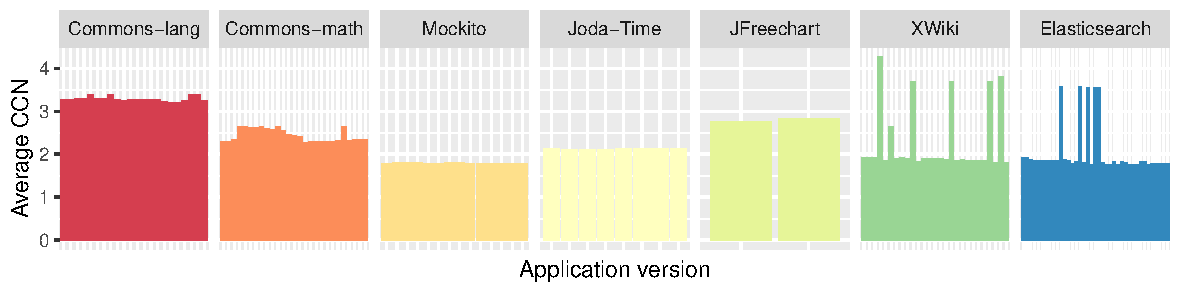
\includegraphics[width=0.98\textwidth]{papers/jcrashpack/benchmark-ccn-per-app-histogram}
  \label{fig:ccnperapp}
  }
  \subfloat[Thousands of Non-Com\-men\-ting Sources Statements (KNCSS)]{
%    	\includegraphics[width=0.80\textwidth]{benchmark-ncss-per-app-boxplot}
    	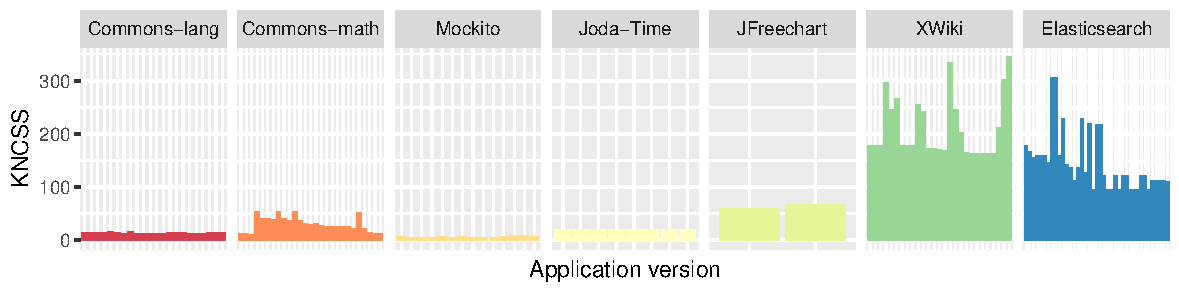
\includegraphics[width=0.98\textwidth]{papers/jcrashpack/benchmark-ncss-per-app-histogram}
    \label{fig:ncssperapp}
  }
  \caption{Complexity and size of the different projects}
  \label{fig:ccnncssperapp}
\end{figure}

Figure \ref{fig:ccnncssperapp} presents the average Cyclomatic Complexity Number (CCN) per method for each project and the Non-Com\-men\-ting Sources Statements (NCSS) per project, ordered by version number, to give an idea of the complexity of a project. Also, Table \ref{tab:benchmark:complexity} gives the number of versions and the average number of non-commenting source statement for each project in \crashpack.
As illustrated in the table and figure, \crashpack contains projects of diverse complexities (the CCN for the least complex project is 1.77, and for the most complex is 3.38) and sizes (the largest project has 177,840 statements, and the smallest one holds 6,060 statements on average), distributed among different versions.

\begin{table*}[t]
	\centering
	\caption{The number of versions and average number of statements ($\overline{NCSS}$) for each project.}
	\label{tab:benchmark:complexity}
	\begin{tabular}{ l | c r } \textbf{Applications} & \textbf{Number of versions} & \textbf{$\overline{NCSS}$}\\
\hline 
\textbf{ Commons-lang } & 22 & 13.38k \\
\textbf{ Commons-math }  & 27 & 29.98k \\
\textbf{ Mockito } & 14 & 6.06k \\
\textbf{ Joda-Time } & 8 & 19.41k \\
\textbf{ JFreechart } & 2 & 63.01k \\
\textbf{ XWiki } & 32 & 177.84k \\
\textbf{ Elasticsearch } & 46 & 124.36k \\
\textbf{ Total } & 151 & 62.01k \\
\end{tabular}
\end{table*}

\begin{table*}[t]
	\centering
	\caption{Number of stack traces (\textit{st}), total number of frames (\textit{fr}), and average number of frames ($\overline{fr}$) and standard deviation ($\sigma$) per stack trace for the different exceptions: NullPointerException (NPE), IllegalArgumentException (IAE), ArrayIndexOutOfBoundsException (AIOOBE), ClassCastException (CCE), StringIndexOutOfBoundsException (SIOOBE), IllegalStateException (ISE), and other exceptions types (Other). }
	\label{tab:benchmark}
%	\input{benchmark-exceptionsapps-table.tex}
    \begin{scriptsize}
	% NullPointerException (NPE), IllegalArgumentException (IAE), ArrayIndexOutOfBoundsException (AIOOBE), ClassCastException (CCE), StringIndexOutOfBoundsException (SIOOBE), IllegalStateException (ISE), Other (Other), 
\begin{tabular}{ l l | r r r r r r r | r } \textbf{Applications} & & \textbf{\rotatebox{90}{ NPE }} & \textbf{\rotatebox{90}{ IAE }} & \textbf{\rotatebox{90}{ AIOOBE }} & \textbf{\rotatebox{90}{ CCE }} & \textbf{\rotatebox{90}{ SIOOBE }} & \textbf{\rotatebox{90}{ ISE }} & \textbf{\rotatebox{90}{ Other }} & \textbf{ Total } \\ 
\hline 
\textbf{ Commons-lang } & \textit{st}  & 5.0 & 3.0 & 2.0 & 0.0  & 6.0 & 0.0  & 6.0 & 22.0\\ 
  & \textit{fr}  & 8.0 & 3.0 & 12.0 & 0.0 & 10.0 & 0.0 & 12.0 & 45.0\\ 
  & $\overline{fr}$  & 1.6 & 1.0 & 6.0 &   & 1.7 &   & 2.0 & 2.0\\ 
 & $\sigma$  & 0.9 & 0.0 & 5.7 &   & 1.0 &   & 1.5 & 2.1\\ 
\hline 
\textbf{ Commons-math } & \textit{st}  & 3.0 & 3.0 & 4.0 & 2.0 & 1.0 & 0.0  & 14.0 & 27.0\\ 
  & \textit{fr}  & 8.0 & 7.0 & 9.0 & 11.0 & 1.0 & 0.0 & 70.0 & 106.0\\ 
  & $\overline{fr}$  & 2.7 & 2.3 & 2.2 & 5.5 & 1.0 &   & 5.0 & 3.9\\ 
 & $\sigma$  & 0.6 & 1.5 & 2.5 & 6.4 & NA &   & 3.0 & 3.0\\ 
\hline 
\textbf{ Mockito } & \textit{st}  & 2.0 & 0.0  & 2.0 & 2.0 & 0.0  & 0.0  & 8.0 & 14.0\\ 
  & \textit{fr}  & 3.0 & 0.0 & 12.0 & 2.0 & 0.0 & 0.0 & 48.0 & 65.0\\ 
  & $\overline{fr}$  & 1.5 &   & 6.0 & 1.0 &   &   & 6.0 & 4.6\\ 
 & $\sigma$  & 0.7 &   & 7.1 & 0.0 &   &   & 3.8 & 4.1\\ 
\hline 
\textbf{ Joda-Time } & \textit{st}  & 0.0  & 3.0 & 0.0  & 0.0  & 0.0  & 0.0  & 5.0 & 8.0\\ 
  & \textit{fr}  & 0.0 & 5.0 & 0.0 & 0.0 & 0.0 & 0.0 & 26.0 & 31.0\\ 
  & $\overline{fr}$  &   & 1.7 &   &   &   &   & 5.2 & 3.9\\ 
 & $\sigma$  &   & 0.6 &   &   &   &   & 1.5 & 2.2\\ 
\hline 
\textbf{ JFreechart } & \textit{st}  & 1.0 & 1.0 & 0.0  & 0.0  & 0.0  & 0.0  & 0.0  & 2.0\\ 
  & \textit{fr}  & 6.0 & 6.0 & 0.0 & 0.0 & 0.0 & 0.0 & 0.0 & 12.0\\ 
  & $\overline{fr}$  & 6.0 & 6.0 &   &   &   &   &   & 6.0\\ 
 & $\sigma$  & NA & NA &   &   &   &   &   & 0.0\\ 
\hline 
\textbf{ XWiki } & \textit{st}  & 20.0 & 4.0 & 0.0  & 6.0 & 1.0 & 0.0  & 20.0 & 51.0\\ 
  & \textit{fr}  & 535.0 & 39.0 & 0.0 & 131.0 & 8.0 & 0.0 & 687.0 & 1400.0\\ 
  & $\overline{fr}$  & 26.8 & 9.8 &   & 21.8 & 8.0 &   & 34.4 & 27.5\\ 
 & $\sigma$  & 33.3 & 3.7 &   & 22.2 & NA &   & 47.0 & 37.0\\ 
\hline 
\textbf{ Elasticsearch } & \textit{st}  & 18.0 & 10.0 & 6.0 & 0.0  & 1.0 & 7.0 & 34.0 & 76.0\\ 
  & \textit{fr}  & 222.0 & 152.0 & 102.0 & 0.0 & 15.0 & 135.0 & 717.0 & 1343.0\\ 
  & $\overline{fr}$  & 12.3 & 15.2 & 17.0 &   & 15.0 & 19.3 & 21.1 & 17.7\\ 
 & $\sigma$  & 9.8 & 9.2 & 18.0 &   & NA & 11.9 & 13.4 & 12.5\\ 
\hline 
 \textbf{Total}  & \textit{st}  & 49.0 & 24.0 & 14.0 & 10.0 & 9.0 & 7.0 & 87.0 & 200.0\\ 
  & \textit{fr}  & 782.0 & 212.0 & 135.0 & 144.0 & 34.0 & 135.0 & 1560.0 & 3002.0\\ 
  & $\overline{fr}$  & 16.0 & 8.8 & 9.6 & 14.4 & 3.8 & 19.3 & 17.9 & 15.0\\ 
 & $\sigma$  & 23.9 & 8.5 & 13.3 & 19.3 & 4.8 & 11.9 & 26.3 & 22.3\\ 
\end{tabular} 
    \end{scriptsize}
\end{table*}

Table \ref{tab:benchmark} shows the distribution of stack traces per exception type for the six most 
common ones, the \textit{Other} category denoting remaining exception types. According to this table, the included stack traces in \crashpack covers different types of the exceptions. Also, they are varied in the size (number of frames): the smallest stack traces have one frame and the largest, a user-defined exception in \textit{Other}, has 175 frames.

\crashpack is extensible and publicly available on GitHub.\footnote{At \url{https://github.com/STAMP-project/JCrashPack}} We provide guidelines to add new crashes to the benchmark and make a pull request to include them in \crashpack master branch.
%
The detailed numbers for each stack trace and its project are available on the \crashpack website.



\section{Running Experiments With ExRunner}
\label{sec:jcrashpack:ExRunner}

\begin{figure}[t]
\centering
\includegraphics[width=0.85\textwidth]{papers/jcrashpack/crashpack-Scheduler}
\caption{\exrunner overview}
\label{fig:exrunner}
\end{figure}

We combine \crashpack with \exrunner, a tool that can be used for running experiments with a given stack trace-based crash reproduction tool. This tool
\begin{inparaenum}[(i)]
\item facilitates the automatic parallel execution of the crash reproduction instances, 
\item ensures robustness in the presence of failures during the crash reproduction failure, and
\item allows to plug different crash reproduction tools to allow a comparison of their capabilities.
\end{inparaenum}

Figure \ref{fig:exrunner} gives an overview of \exrunner architecture.
The \emph{job generator} takes as input the stack traces to reproduce, the path to the Jar files associated to each stack trace, and the configurations to use for the stack trace reproduction tool under study. 
%
For each stack trace, the job generator analyzes the stack frames and discards those with a target method that does not belong to the target system, based on the package name. 
For instance, frames with a target method belonging to the Java SDK or other external dependencies are discarded from the evaluation.
For each configuration and stack trace, the job generator creates a new job description (i.e., a JSON object with all the information needed to run the tool under study) and adds it to a queue. 

To speed-up the evaluation, \exrunner multithreads the execution of the jobs.
The number of threads is provided by the user in the configuration of \exrunner and depends on the resources available on the machine and required by one job execution.
Each thread picks a job from the waiting queue and executes it. 
\exrunner users may activate an observer that monitors the jobs and takes care of killing (and reporting) those that do not show any sign of activity (by monitoring the job outputs) for a user-defined amount of time.
The outputs of every job are written to separate files, with the generated test case (if any) and the results of the job execution (output results from the tool under study).

For instance, when used with \evocrash, the log files contain data about the target method, progress of the fitness function value during the execution, and branches covered by the execution of the current test case (in order to see if the line where the exception is thrown is reached). 
In addition, the results contain information about the progress of search (best fitness function, best line coverage, and if the target exception is thrown), and number of fitness evaluations performed by \evocrash in an output CSV file. 
If \evocrash succeeds to replicate the crash, the generated test is stored separately.

As mentioned by Fraser et al. \cite{FA13challenges}, any research tool developed to generate test cases may face specific challenges. 
One of these is long (or infinite) execution time of the test during the generation process. 
To manage this problem, \evosuite uses a timeout for each test execution, but sometimes it fails to kill sub-processes spawned during the search \cite{FA13challenges}.
We also experienced \evocrash freezing during our evaluation. 
%
In order to handle this problem, \exrunner creates an observer to check the status of each thread executing an \evocrash instance.
If one \evocrash execution does not respond for $10$ minutes (66\% of the expected execution time), the Python script kills the \evocrash process and all of its spawned threads. 

Another challenge relates to garbage collection: we noticed that, at some point of the execution, one job (i.e., one JVM instance) allocated all the CPU cores for the execution of the garbage collector, preventing other jobs to run normally. 
Moreover, since \evocrash allocates a large amount of heap space to each sub-process responsible to generate a new test case (since the execution of the target application may require a large amount of memory) \cite{FA13challenges}, the garbage collection process could not retrieve enough memory and got stuck, stopping all jobs on the machine.
To prevent this behaviour, we set \emph{-XX:ParallelGCThreads} JVM parameter to 1, enabling only one thread for garbage collection, and limited the number of parallel threads per machine, depending on the maximal amount of allocated memory space. 
We set the number of active threads to 5 for running on virtual machines, and 25 for running on two powerful machines. 
Using the logging mechanism in \evocrash, we are able to see when individual executions ran out of memory.

\exrunner is available together with \crashpack.\footnote{See \url{https://github.com/STAMP-project/ExRunner-bash}.}
It has been used to perform benchmarking for search-based crash reproduction approaches, both \evocrash and \botsing (an open-source search-based crash reproduction framework for assessing the new techniques introduced in this thesis), yet it has been designed to be extensible to other available stack trace reproduction tools using a plugin mechanism. 
Integrating another crash reproduction tool requires the definition of two handlers, called by \exrunner: one to run the tool with the inputs provided by \exrunner (i.e. the stack trace, the target frame, and the classpath of the software under test); and one to parse the output produced by the tool to pick up relevant data (e.g., the final status of the crash reproduction, progress of the tool during the execution, \textit{etc}.). 
Relevant data are stored in a CSV file, readily available for analysis.\footnote{ The \exrunner documentation includes a detailed tutorial describing how to proceed, available at \url{https://github.com/STAMP-project/EvoCrash-JCrashPack-application\#run-other-crash-replication-tools-with-exrunner}.}



\section{Application To \evocrash: Setup}
\label{sec:jcrashpack:evocrashevalsetup}

Having \crashpack available allowed us to perform an extensive evaluation of \evocrash, a state-of-the-art tool in search-based crash replication~\cite{Soltani2018a}.
Naturally, our first research question deals with the capability of \evocrash to reproduce crashes from \crashpack: 
%
\begin{itemize}
    \item[\textbf{RQ$_{1.1}$}] \textit{To what extent can \evocrash reproduce crashes from \crashpack?}
\end{itemize}
%
Since the primary goal of our evaluation is to identify current limitations, we refine the previous research question to examine which frames of the different crashes \evocrash is able to reproduce:
%
\begin{itemize}
    \item[\textbf{RQ$_{1.2}$}] \textit{To what extent can \evocrash reproduce the different frames of the crashes from \crashpack?}
\end{itemize}
%
The diversity of crashes in \crashpack also allows us to investigate how certain types of crashes affect reproducibility.
Thus, we investigate whether the exception type and  the project nature have an influence on the reproduction rate:
\begin{itemize}
   \item[\textbf{RQ$_{2.1}$}] \textit{How does project type influence performance of \evocrash for crash reproduction?}
\end{itemize}
In addition, different types of projects might have impact on how costly it is to reproduce the reported crashes for them.
The second research question studies the influence of the exception and project type on the performance of \evocrash:
%
\begin{itemize}
   \item[\textbf{RQ$_{2.2}$}] \textit{How does exception type influence performance of \evocrash for crash reproduction?}
\end{itemize}
%
Finally, we seek to understand why crashes could \emph{not} be reproduced:
%
\begin{itemize}
    \item[\textbf{RQ$_{3}$\phantom{y}}] \textit{What are the main challenges that impede successful search-based crash reproduction?}
\end{itemize}

\subsection{Evaluation Setup}
\label{se:evalsetup}

\paragraph{Number of executions.}

Due to the randomness of Guided Genetic Algorithm in \evocrash, we executed the tool multiple times on each frame. 
The number of executions has to strike a balance between the threats to external validity (i.e., the number of stack traces considered) and the statistical power (i.e., number of runs) \cite{Fraser2014b, Arcuri2014}. 
In our case, we do not compare \evocrash to other tools (see for instance Soltani \etal \cite{soltani2017, Soltani2018a}), but rather seek to identify challenges for crash reproduction. 
Hence we favor external validity by considering a larger amount of crashes compared to previous studies \cite{Soltani2018a} and ran \evocrash 10 times on each frame. In total, we executed 18,590 \evocrash runs.

\paragraph{Search parameters.}

We used the default parameter values \cite{Arcuri2011a, Fraser2014b} with the following additional configuration options: 
we chose to keep the reflection mechanisms, used to call private methods, deactivated.
The rationale behind this decision is that using reflection can lead to generating invalid objects that break the class invariant \cite{Liskov2000} during the search, which results in test cases helplessly trying to reproduce a given crash \cite{Chen2015}.

After a few trials, we also decided to activate the implementation of functional mocking available from \evosuite \cite{arcuri2017private} in order to minimize possible risks of environmental interactions on crash reproduction.
Functional mocking works as follows: when, in a test case, a statement that requires new specific objects to be created (as parameters of a method call for instance) is inserted, either a plain object is instantiated by invoking its constructor, or (with a defined probability, left to its default value in our case) a mock object is created. This mock object is then refined using \texttt{when}-\texttt{thenReturn} statements, based on the methods called during the execution of the generated test case. Functional mocking is particularly useful in the cases where the required object cannot be successfully initialized (for instance, if it relies on environmental interactions or if the constructor is accessible only through a factory). 

Investigating the impact of those parameters and other parameters (e.g., cross\-over rate, mutation rate, etc. to overcome the challenges as identified in \textbf{RQ$_3$}) is part of our future work. 

\paragraph{Search budget.}

Since our evaluation is executed in parallel on different machines, we choose to express the budget time in terms of number of fitness evaluations: i.e., the number of times the fitness function is called to evaluate a generated test case during the execution of the guided generic algorithm. We set this number to 62,328, which corresponds to the average number of fitness evaluations performed by \evocrash when running it during 15 minutes on each frame of a subset of 4 randomly selected stack traces on one out of our two machines. Both of the machines have the same configuration: A cluster running Linux Ubuntu 14.04.4 LTS with 20 CPU-cores, 384 GB memory, and a 482 GB hard drive.

We partitioned the evaluation into two, one per available machine: all the stack traces with the same kind of exception have been run on one machine for 10 rounds.
%
For each run, we measure the number of fitness evaluations needed to achieve reproduction (or the exhaustion of the budget if \evocrash fails to reproduce the crash) and the best fitness value achieved by \evocrash (0 if the crash is reproduced and higher otherwise).
%
The whole process is managed using \exrunner.
The evaluation itself was executed during 10 days on our 2 machines.

\section{Application To \evocrash: Results}
\label{sec:jcrashpack:evocrashevalresults}

In this section, we answer the first two research questions on the extent to which the selected crashes and their frames were reproduced and the impact of the project and the exception type on the performance of \evocrash.
%
We detail the results by analyzing the outcome of \evocrash  in a majority of 10 executions for each frame of each stack trace. We classify the outcome of each execution in one of the five following categories:
\begin{itemize}
\item[] \textbf{reproduced:} when \evocrash generated a test that successfully reproduced the stack trace at the given frame level; 
\item[]\textbf{ex. thrown:} when \evocrash generated a test that cannot fully reproduce the stack trace, but covers the target line and throws the desired exception. The frames of the exception thrown, however, do not contain all the original frames;
\item[]\textbf{line reached:} when  \evocrash generated a test that covers the target line, but does not throw the desired exception;
\item[]\textbf{line not reached:} when none of the tests produced by \evocrash could cover the target line within the available time budget;
and \item[]\textbf{aborted:} when \evocrash could not generate an initial population to start the search process.
\end{itemize}
%
Each outcome denotes a particular state of the search process. For the \emph{reproduced} frames, \evocrash could generate a crash-reproducing test within the given time budget (here, 62,328 fitness evaluations). For the frames that could not be reproduced, either \evocrash exhausted the time budget (for \emph{ex. thrown}, \emph{line reached}, and \emph{line not reached} outcomes) or could not perform the guided initialization (i.e., generate at least one test case with the target method) and did not start the search process (\emph{aborted} outcomes). 
For instance, if the class in the target frame is abstract, \evocrash may fail to find an adequate implementation of the abstract class to instantiate an object of this class during the guided initialization.

\subsection{Crash Reproduction Outcomes (RQ1)}

For \textbf{RQ$_1$},  we first look at the reproduced and non-reproduced crashes to answer \textbf{RQ$_{1.1}$}. 
If \evocrash was successful in reproducing any frame of a stack trace in a majority of 10 executions, we count the crash as a \textbf{reproduced crash}. Otherwise, we count the crash as \textbf{not reproduced}.
%
To answer \textbf{RQ$_{1.2}$}, we detail the results by analyzing the outcome of \evocrash  in a majority of 10 executions for each frame of each stack trace. 

\begin{figure}[t]
	\centering
%	\includegraphics[width=0.90\textwidth]{rq1_compact.pdf}
	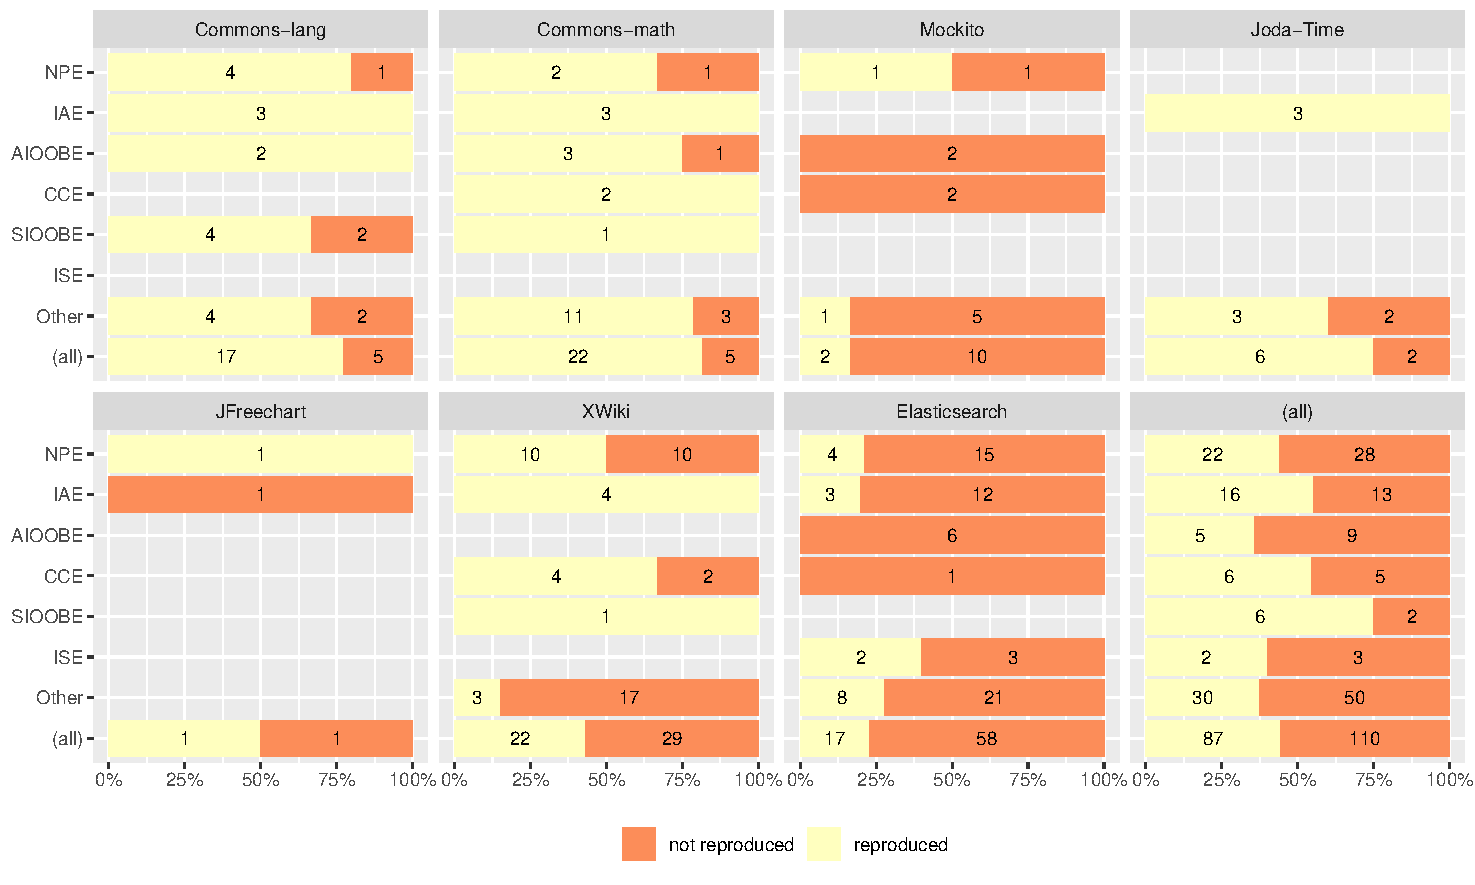
\includegraphics[width=\textwidth]{papers/jcrashpack/rq1_crashes.pdf}
	\caption{Reproduction outcome for the different crashes}
	\label{fig:rq1crashes}
\end{figure}

Figure \ref{fig:rq1crashes} shows the number of reproduced and not reproduced crashes for each project (and all the projects) and type of exception.
\evocrash is successful in reproducing the majority of crashes (more than 75\%) from \textit{Commons-lang}, \textit{Commons-math}, and \textit{Joda-Time}. 
For the other projects, \evocrash reproduced 50\% or less of the crashes, with only 2 out of 12 crashes reproduced for \textit{Mockito}.
%
Crashes with an \textit{IllegalArgumentException} are the most frequently reproduced crashed: 16 out of 29 (55\%).

\begin{figure*}[t]
	\centering
	\subfloat[In each type of exception]{
	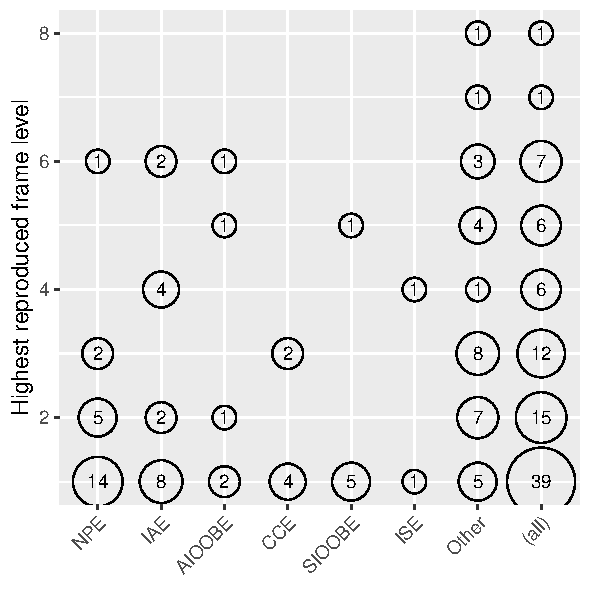
\includegraphics[width=0.48\textwidth]{papers/jcrashpack/rq1_framelvlex.pdf}
	\label{fig:rq1_framelvlex}
	}
	%
	\subfloat[In each type of application]{
	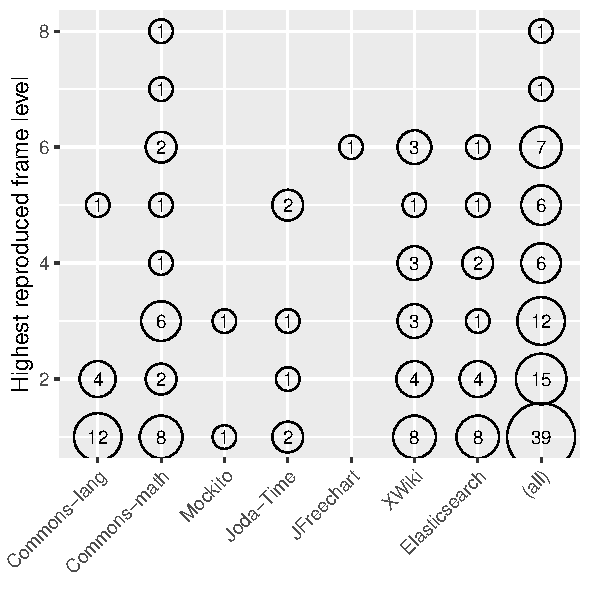
\includegraphics[width=0.48\textwidth]{papers/jcrashpack/rq1_framelvlapp.pdf}
	\label{fig:rq1_framelvlapp}
	}
	\caption{Highest reproduced frame levels}
	\label{fig:highestframe}
\end{figure*}

Before detailing the results of each frame of each crash, we first look at the frame levels that could be reproduced. Figure \ref{fig:highestframe} presents for the 87 stack traces that could be reproduced, the distribution of the highest frame level that could be reproduced for the different crashes for each type of exception (in Figure \ref{fig:rq1_framelvlex}) and each application (in Figure \ref{fig:rq1_framelvlapp}).
As we can see, \evocrash replicates lower frame levels more often than higher levels. 
For instance, for 39 out of  the 87 reproduced stack traces, \evocrash could not reproduce frames beyond level 1 and could reproduce frames up to level 5 for only 9 crashes. 

Figure \ref{fig:rq1_framelvlex} indicates that \evocrash can replicate only the first frame in 14 out of 22 NPE crashes, while there is only one NPE crash for which \evocrash could reproduce a frame above level 3. 
In contrast, it is more frequent for \evocrash to reproduce higher frame levels of IAE stack traces: the highest reproduced frames in 6 out of 16 IAE crashes are higher than 3.
%
Those results suggest that, when trying to reproduce a crash, propagating an illegal argument value trough a chain of method calls (i.e., the frames of the stack trace) is easier than propagating a \texttt{null} value. 
%
According to Figure \ref{fig:rq1_framelvlapp}, \evocrash can reproduce frames higher than 6 only for \textit{Commons-math} crashes. The highest reproduced frames in most of the reproduced crashes in this project are higher than level 2 (12 out of 22). 
In contrast, for \textit{Elasticsearch} the highest reproduced frame is 1 in most of the crashes.

Both the number of crashes reproduced and the highest level at which crashes could be reproduced confirm the relevance of our choice to consider crashes from XWiki and Elasticsearch, for which the average number of frames (resp. 27.5 and 17.7) is higher than for Defects4J projects (at most 6.0 for JFreeChart), as they represent an opportunity to evaluate and understand current limitations. 

\subsubsection{Frames reproduction outcomes} 

\begin{figure}[t]
	\centering
%	\includegraphics[width=0.90\textwidth]{rq1_compact.pdf}
	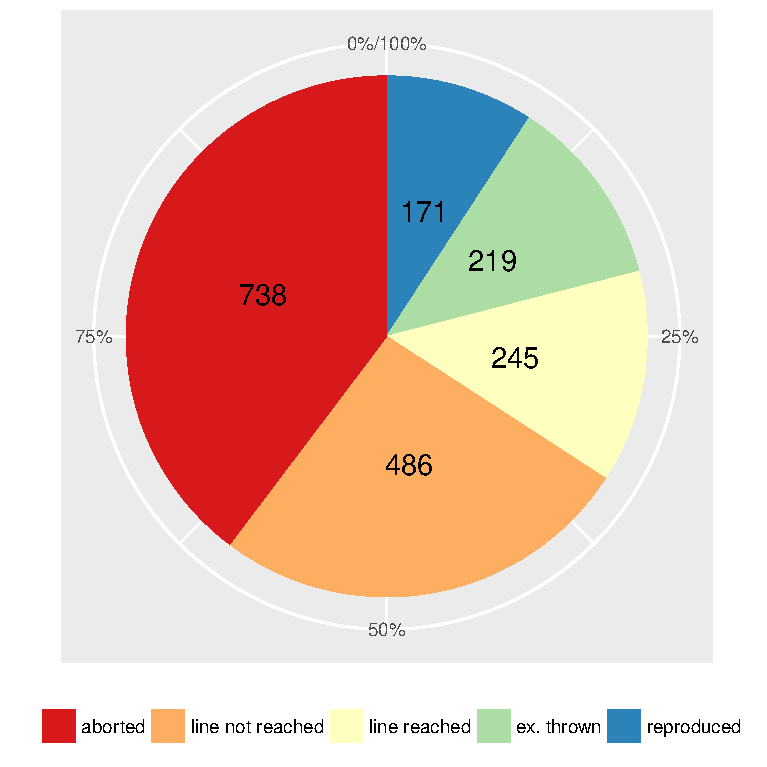
\includegraphics[width=8cm]{papers/jcrashpack/rq1_summary.pdf}
	\caption{An overview of the reproduction outcome}
	\label{fig:rq1summary}
\end{figure}

\begin{figure}[t]
	\centering
%	\includegraphics[width=0.90\textwidth]{rq1_compact.pdf}
	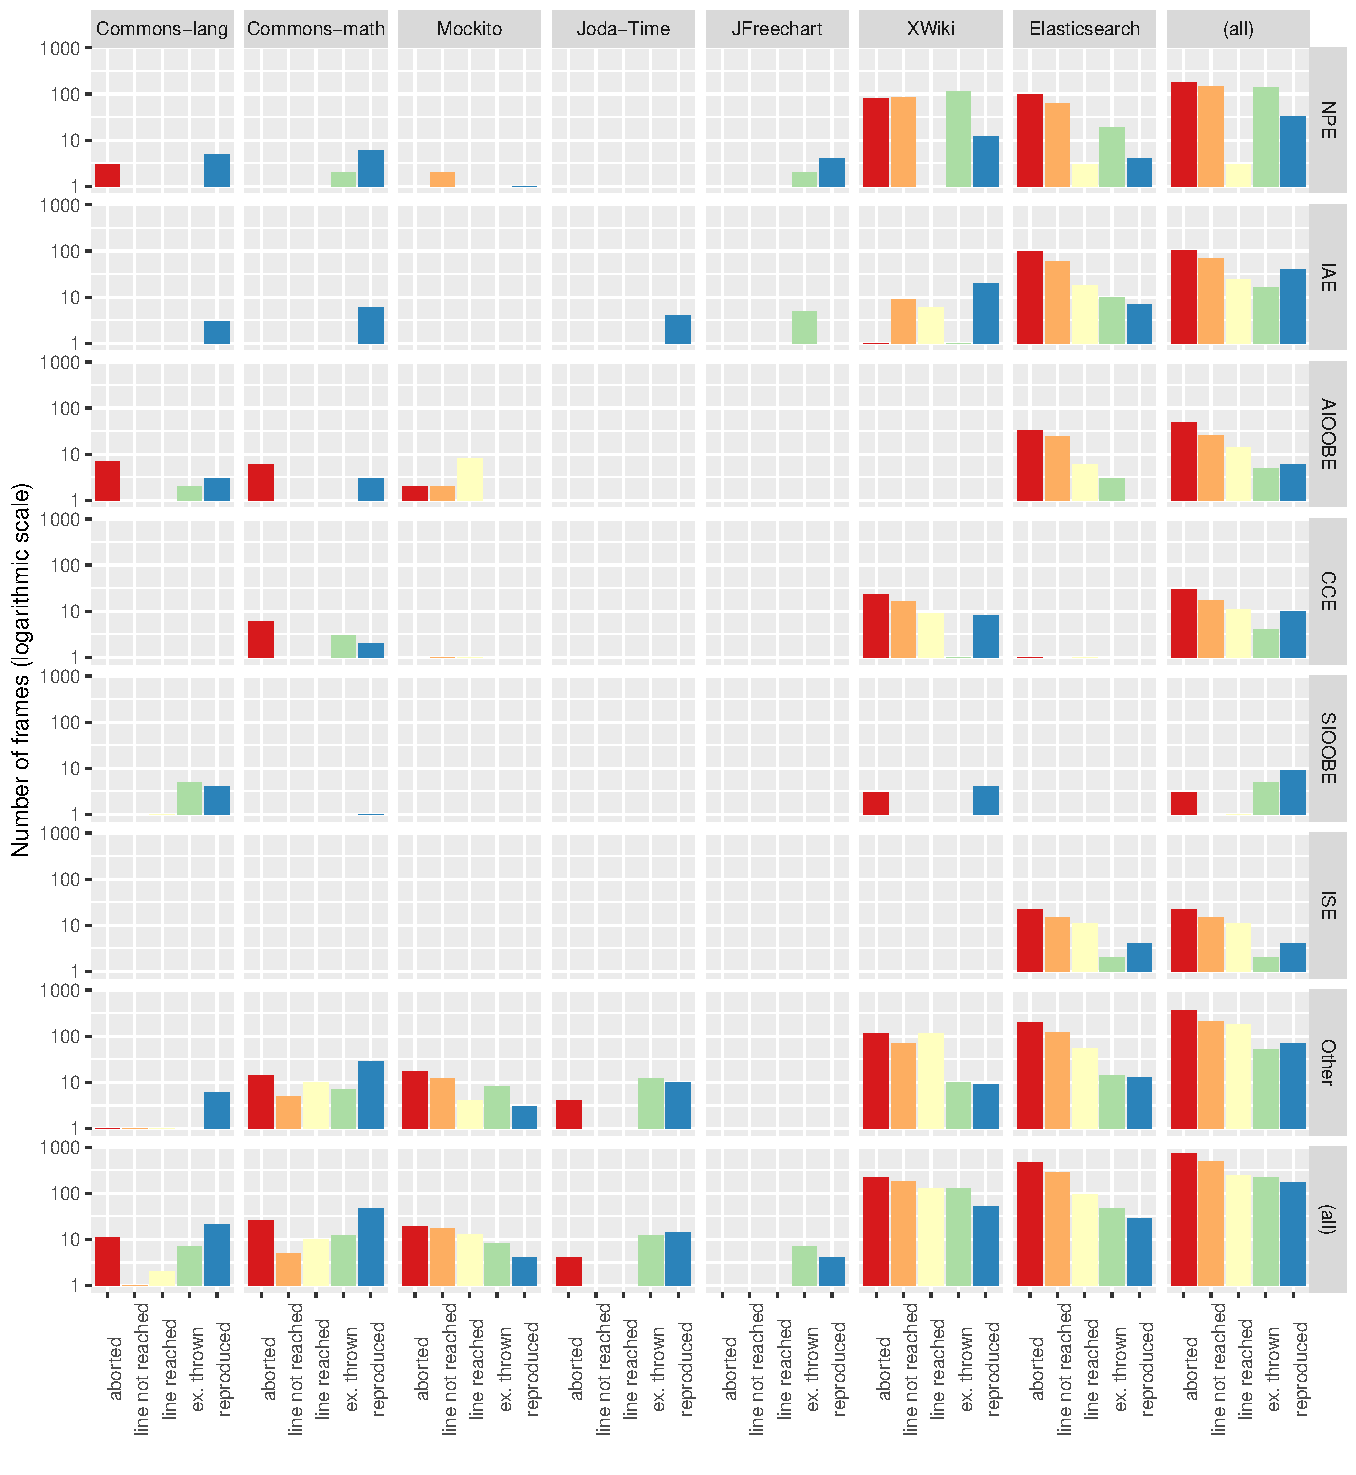
\includegraphics[width=\textwidth]{papers/jcrashpack/rq1_all.pdf}
	\caption{Detailed reproduction outcome for the different frames.}
	\label{figure:outcomecomp}
\end{figure}

To answer \textbf{RQ$_{1.2}$}, we analyze the results for each frame individually.
%
Figure~\ref{fig:rq1summary} presents a summary of the results with the number of frames for the different outcomes. Figure \ref{figure:outcomecomp} details the same results by application and exception. 

Overall, we see in Figure \ref{fig:rq1summary} that \evocrash reproduced 171 frames (out of 1,859), from 87 different crashes (out of 200) in the majority of the ten rounds. If we consider the frames for which \evocrash generated a crash-reproducing test at least once in the ten rounds, the number of reproduced frames increases to 201 (from 96 different crashes).
%
In total, \evocrash exhausted the time budget for 950 frames: 219 with a test case able to throw the target exception, 245 with a test case able to reach the target line, and 486 without a test case able to reach the line. 
\evocrash aborted the search for 738 frames, 455 of which were from Elasticsearch, the application for which \evocrash had the most difficulties to reproduce a stack trace. 

Figure~\ref{figure:outcomecomp} details the results by applications (columns) and exceptions (lines). The last line (resp. column), denoted \textit{(all)}, provides the global results for the applications (resp. exceptions). In the remainder of this section, we discuss the results for the different applications and exceptions. 

\subsubsection{Defects4J applications}

For the Defects4J applications, presented in the first five columns in Figure~\ref{figure:outcomecomp}, in total, 90 (out of 244) of the frames from 48 (out of 71) different crashes were \emph{reproduced}. 
For 94 frames, \evocrash exhausted the time budget (46 \emph{ex. thrown}, 25 \emph{line reached}, and 23 \emph{line not reached}) and \emph{aborted} for 60 frames from the Defects4J projects. 

In particular, only 4 frames out of 61 frames for Mockito were successfully reproduced.
For instance, \evocrash could not reproduce \texttt{MOCKITO-4b}, which has only one frame.
From our evaluation, we observe that one very common problem when trying to reproduce a \textit{ClassCastException} is to find which class should be used to trigger the exception.
%
\begin{lstlisting}[language=Java]
public void noMoreInteractionsWantedInOrder(Invocation undesired){
  throw new VerificationInOrderFailure(join( ...,
		"..." + undesired.getMock() + "':", ...));
}
\end{lstlisting}
%
The exception happens when the \texttt{undesired.getMock()} call returns an object that cannot be cast to \texttt{String}.
During the search, \evocrash mocks the \texttt{undesired} object and assigns some random value to return when the \texttt{getMock} method is called. 
\evocrash generates a test able to cover the target line, but failing to trigger an exception. 
Since the signature of this method is \texttt{Object getMock()}, \evocrash assigns only random \texttt{Object} values to return, where, from the original stack trace, a \texttt{Boolean} value is required to trigger the exception.

\subsubsection{XWiki and Elasticsearch}

XWiki is one of the industrial open source cases in the evaluation, for which 53 (out of 706) frames were successfully \emph{reproduced}, 430 could not be reproduced with the given time budget (125 \emph{ex. thrown}, 127 \emph{line reached}, and 178 \emph{line not reached}), and 223  \emph{aborted} during the generation of the initial population.
%
\evocrash \emph{reproduced} only 28 (out of 909) frames from Elasticsearch, for which, the majority of frames (455) \emph{aborted}  during the generation of the initial population. However, \evocrash was able to start the search for 426 frames (48 \emph{ex. thrown}, 93 \emph{line reached}, and 285 \emph{line not reached}).

\paragraph{Variability of the reproductions.}

We also observed that XWiki and Elasticsearch have the highest variability in their outcomes. 
For XWiki (resp. Elasticsearch), 4 (resp. 3) frames that could be reproduced in a majority of time could however not be reproduced 10 out of 10 times, compared to 2 frames for Commons-lang and Commons-math. 
This could indicate a lack of guidance in the current fitness function of \evocrash. 
For instance, for the Elasticsearch crash ES-26833, \evocrash could only reproduce the third frame 4 times out of 10 and was therefore not considered as reproduced. 
After a manual inspection, we observed that \evocrash gets stuck after reaching the target line and throwing the expected exception. 
From the intermediate test cases generated during the search, we see that the exception is not thrown by the target line, but a few lines after. 
Since the fitness value improved, \evocrash got stuck into a local optima, hence the lower frequency of reproduction  for that frame.\footnote{A detailed analysis is available at \url{https://github.com/STAMP-project/EvoCrash-JCrashPack-application/blob/master/results/manual-analysis/Elasticsearch/ES-26833.md}}
Out future work includes improvement of the guidance in the fitness function and a full investigation of the fitness landscape to decrease the variability of \evocrash outcomes. 


\paragraph{Importance of large industrial applications.}

Compared to Defects4J and XWiki applications, the crash reproduction rate drops from 36.9\% for Defects4J, to 7.5\% for XWiki, and only 3\% for Elasticsearch. Those results emphasize the importance of large industrial applications for the assessment of search-based crash reproduction and enforce the need of context-driven software engineering research to identify relevant challenges \cite{Briand2017a}. 

Additionally to the larger variability of reproduction rate, we observe that frequent use of \textit{Java generics} and \textit{static initialization}, and most commonly, automatically generating suitable input data that resembles \texttt{http} requests are among the major reasons for the encountered challenges for reproducing Elasticsearch crashes.
In Section~\ref{sec:jcrashpack:challenges} we will describe \textbf{14} categories of challenges that we identified as the underlying causes for the presented execution outcomes.

\subsubsection{Exceptions}

The lines in Figure~\ref{figure:outcomecomp} presents the outcomes for the different exceptions. In particular, NPE, IAE, AIOOBE, and CCE are the most represented exceptions in \crashpack. For those exceptions, \evocrash could reproduce, respectively, 32 (out of 499), 40 (out of 250), 6 (out of 99), and 10 (out of 72) frames. Looking at the reproduction frequency, IAE is the most frequently reproduced exception (16\%), followed by CCE (13.8\%), NPE (6.4\%), and AIOOBE (6\%). 

This contrast with the number of frames for which \evocrash aborted the search, where NPE has the lowest frequency (181 frames, 36.2\%), followed by IAE (101 frames, 40.4\%), CCE (30 frames, 41.6\%), and AIOOBE (48 frames, 48.4\%). Interestingly, those numbers show that \evocrash is able to complete the guided initialization for NPEs more often than for other exceptions. 

Figure~\ref{figure:outcomecomp} also shows that the number of test cases that reach the line is low for NPEs, meaning that whenever \evocrash generates at test able to cover the line (\emph{line reached}), the evolution process will be able to progress and generate another test that throws an exception (\emph{ex. thrown}).


\paragraph{\textbf{Summary (RQ$_1$)} To what extent can \evocrash reproduce crashes from \crashpack, and how far it can proceed in the stack traces?}
%
Overall, \evocrash reproduced 171 frames (out of 1,859 - 9\%), from 87 different crashes (out of 200 - 43.5\%) in a majority out of 10 executions. Those numbers climb to 201 frames (10.8\%) from 96 crashes (48\%) if we consider at least one reproduction in one of the 10 executions.
%
In most of the reproduced crashes, \evocrash can only reproduce the first two frames. It indicates that since \evocrash needs higher accuracy in setting the state of the software under test for reproducing higher frames, increasing the length of the stack trace reduces the chance of this tool for crash reproduction. 
%
When looking at larger industrial applications, the crash reproduction rates drop from 36.9\% for Defects4J to 7.5\% for XWiki and 3\% for Elasticsearch.
%
The most frequently reproduced exceptions are IllegalArgumentExceptions. The exceptions for which \evocrash is the most frequently able to complete the guided initialization are NullPointerExceptions.


\subsection{Impact of Exception Type and Project on Performance (RQ2)}

To identify the distribution of fitness evaluations per exception type and project, we filtered the \emph{reproduced} frames out of the 10 rounds of execution.
Tables~\ref{tab:appstats} and~\ref{tab:typestats} present the statistics for these executions, grouped by application and exception types, respectively.

\begin{table*}[t]
\caption{Statistics for the average number of fitness evaluations for the \textit{reproduced} frames (\textbf{fr}) belonging to different stack traces (\textbf{st}), grouped by \textbf{applications}, out of 10 rounds of execution.
The confidence Interval (\textbf{CI}) is calculated for the median bootstrapping with \textit{100,000} runs, at a 95\% confidence level.}
\label{tab:appstats}
\begin{scriptsize}
\begin{tabularx}{0.945\textwidth}{ l r r r r r r r r } 
\hline 
\textbf{Applications} & \textbf{st} & \textbf{fr}& \textbf{Min} & \textbf{Lower Quart.} & \textbf{Median CI} & \textbf{Med.} & \textbf{Upper Quart.} & \textbf{Max} \\ 
\hline 
\textbf{ Com.-lang } & 19  & 213  & 1  & 2.0  & [ 5.0 ,22.0] & 15.0  & 237.0  & 52,240  \\ 
\textbf{ Com.-math } & 24  & 471  & 1  & 13.0  & [ 124.0 ,211.0] & 178.0  & 1,046.5  & 58,731  \\ 
\textbf{ Mockito } & 2  & 40  & 1  & 1.0  & [ 1.0 ,1.0] & 1.0  & 5.2  & 138  \\ 
\textbf{ Joda-Time } & 6  & 138  & 1  & 15.5  & [ 79.1 ,369.0] & 253.5  & 1,290.2  & 40,189  \\ 
\textbf{ JFreechart } & 1  & 41  & 1  & 10.0  & [ -292.0 ,350.0] & 221.0  & 1,188.0  & 20,970  \\ 
\textbf{ XWiki } & 25  & 531  & 1  & 2.5  & [ 14.0 ,30.0] & 23.0  & 209.0  & 34,089  \\ 
\textbf{ Elasticsearch } & 19  & 287  & 1  & 4.0  & [ 5.0 ,32.0] & 23.0  & 125.0  & 17,461  \\ 
\hline 
\textbf{Total} & 96  & 1721  & 1  & 4.0  & [ 34.0 ,59.0] & 48.0  & 534.0  & 58,731  \\ 
\hline 
\end{tabularx} 

\end{scriptsize}
\end{table*}

\begin{table}[t]
\caption{Statistics for the average number of fitness evaluations for the \textit{reproduced} frames (\textbf{fr}) belonging to different stack traces (\textbf{st}), grouped by \textbf{exceptions}, out of 10 rounds of execution.
Confidence Interval (\textbf{CI}) is calculated for median with bootstrapping with \textit{100,000} runs, at 95\% confidence level.}
\label{tab:typestats}
\begin{scriptsize}
\begin{tabularx}{0.94\textwidth}{ l r r r r r r r r} 
\hline 
\textbf{Applications} & \textbf{st} & \textbf{fr}& \textbf{Min} & \textbf{Lower Quart.} & \textbf{Median CI} & \textbf{Med.} & \textbf{Upper Quart.} & \textbf{Max} \\ 
\hline 
\textbf{ NPE } & 26  & 330  & 1  & 6.0  & [ 9.0 ,63.0] & 44.5  & 220.0  & 34,089  \\ 
\textbf{ IAE } & 16  & 399  & 1  & 2.0  & [ 7.0 ,12.0] & 10.0  & 49.0  & 38,907  \\ 
\textbf{ AIOOBE } & 5  & 58  & 1  & 15.5  & [ 252.0 ,1,104.5] & 675.0  & 1,671.2  & 53,644  \\ 
\textbf{ CCE } & 6  & 103  & 1  & 6.5  & [ 74.0 ,210.0] & 120.0  & 560.0  & 10,197  \\ 
\textbf{ SIOOBE } & 8  & 95  & 1  & 12.5  & [ 122.0 ,945.0] & 505.0  & 2,326.0  & 52,240  \\ 
\textbf{ ISE } & 2  & 42  & 1  & 1.0  & [ 1.0 ,3.0] & 2.0  & 105.8  & 1,138  \\ 
\textbf{ Other } & 33  & 694  & 1  & 7.0  & [ 99.0 ,139.0] & 125.5  & 825.0  & 58,731  \\ 
\hline 
\textbf{Total} & 96  & 1721  & 1  & 4.0  & [ 34.0 ,59.0] & 48.0  & 534.0  & 58,731  \\ 
\hline 
\end{tabularx} 

\end{scriptsize}
\end{table}

We filtered out the frames that were not reproduced to analyze the impact of project and exception types on the average number of fitness evaluations and, following recommendations by Arcuri and Briand~\cite{Arcuri2014}, we replaced the test of statistical difference by a confidence interval.
For both groups, we calculated confidence intervals with a  $95\%$ confidence level for medians with bootstrapping with $100,000$ runs.\footnote{We used the \textit{boot} function from the \textit{boot} library in R to compute the \textit{basic} intervals with bootstrapping. See \url{https://github.com/STAMP-project/EvoCrash-JCrashPack-application/tree/master/results} to reproduce the statistical analysis.}

As Table~\ref{tab:appstats} shows, for four projects (Commons-lang, Mockito, XWiki, and Elasticsearch) the median number of fitness evaluations is low.
On the contrary, the cost of crash reproductions for Commons-math, Joda-Time, and JFreechart are  higher in comparison to the rest of projects.
By comparing those results with the projects sizes reported in Table \ref{tab:benchmark:complexity}, where the largest projects are XWiki (with $\overline{NCSS}=177.84k$) and Elasticsearch (with $\overline{NCSS}=124.36k$), we observe that the effort required to reproduce a crash cannot be solely predicted by the project size. 
This is consistent with the intuition that the difficulty of reproducing a crash only depends on the methods involved in the stack trace.

Similarly, according to Figure \ref{fig:ccnperapp}, the average CCN for Mockito, XWiki, and Elasticsearch is lower compared to other projects. 
Table~\ref{tab:appstats} shows that reproducing crashes from these projects is less expensive, and that reproducing crashes from Commons-math, Joda-Time, and JFreechart, which all have higher average CCN, is more expensive.
We also observe that the average CCN for Commons-lang is high, however, contradicting the intuition that crashes from projects higher CCN are more expensive to reproduce, the cost for reproducing crashes in Commons-lang is low compared to other projects.
%
This can be explained by the levels of the frames reproduced by \evocrash: according to Figure \ref{fig:highestframe}, the average level of the reproduced frames in the crashes from Commons-lang is low compared to the other projects and, as we discussed in the previous section, reproducing crashes with fewer frames is easier for \evocrash.

In general, we observe that the performance of \evocrash depends on the complexity of the project and the frame level in the stack trace. Future work includes further investigations to determine which other factors (e.g., code quality) can influence \evocrash performance. 

From Table~\ref{tab:typestats}, we observe that for \textit{CCE}, \textit{SIOOBE}, and \textit{AIOOBE}, the cost of generating a crash-reproducing test case is high, while for \textit{NPE}, \textit{IAE}, and \textit{ISE}, the cost is lower.
One possible explanation could be that generating input data which is in a suitable state for causing cast conflicts, or an array which is in the right state to be accessed by an illegal index is often non-trivial.

In contrast, to trigger an NPE, it is often enough to return a \texttt{null} value not checked by the crashing method.
For example, Listing~\ref{list:NPEexample} shows the stack trace of CHART-4b, a crash from the JFreeChart application.
The crash happens at line \ref{line:NPEcode:crash} of the \texttt{createScatterPlot} method presented in Listing~\ref{list:NPEcode}. 
Listing~\ref{list:NPEtest} shows the test case generated by \evocrash that reproduces the 6th frame (line 6 in Listing~\ref{list:NPEexample}) of the stack trace. 
First, the test initializes the mocks used as mandatory parameters values (from line \ref{line:NPEtest:mock1} to \ref{line:NPEtest:mock2}), before calling the \texttt{createScatterPlot} method (at line \ref{line:NPEtest:crashcall}). The \texttt{ds} \texttt{XYDataset} mock is used along the various calls (from line \ref{line:NPEexample:frame6} to \ref{line:NPEexample:frame1} in Listing~\ref{list:NPEexample}), up to the method \texttt{getDataRange} presented in Listing~\ref{list:XYPlot} that triggers the NPE at line \ref{line:XYPlot:NPE}. In our case, the \texttt{null} value is returned by the \texttt{getRendererForDataset} call with the propagated \texttt{ds} mock at line \ref{line:XYPlot:null}.

\begin{lstlisting}[frame=tb,
  caption={Stack trace for the crash CHART-4b},
  label=list:NPEexample,
  captionpos=t,
  numbers=left,
  firstnumber=0]
java.lang.NullPointerException
	at org.jfree.chart.plot.XYPlot.getDataRange(XYPlot.java:4493)  (*@\label{line:NPEexample:frame1}@*)
	at org.jfree.chart.axis.NumberAxis.autoAdjustRange(NumberAxis.java:434)
	at org.jfree.chart.axis.NumberAxis.configure(NumberAxis.java:417)
	at org.jfree.chart.axis.Axis.setPlot(Axis.java:1044)
	at org.jfree.chart.plot.XYPlot.<init>(XYPlot.java:660)
	at org.jfree.chart.ChartFactory.createScatterPlot(ChartFactory.java:1490) (*@\label{line:NPEexample:frame6}@*)
\end{lstlisting}

\begin{lstlisting}[frame=tb,
  caption={Code excerpt from JFreeChart \texttt{ChartFactory.java}},
  label=list:NPEcode,
  captionpos=t,
  language=Java,
  numbers=left,
  firstnumber=1478]
public static JFreeChart createScatterPlot(String title, String xAxisLabel,
    String yAxisLabel, XYDataset dataset, PlotOrientation orientation,
    boolean legend, boolean tooltips, boolean urls) {

 if (orientation == null) {
  throw new IllegalArgumentException("Null 'orientation' argument.");
 }
 NumberAxis xAxis = new NumberAxis(xAxisLabel);
 xAxis.setAutoRangeIncludesZero(false);
 NumberAxis yAxis = new NumberAxis(yAxisLabel);
 yAxis.setAutoRangeIncludesZero(false);

 XYPlot plot = new XYPlot(dataset, xAxis, yAxis, null);  (*@\label{line:NPEcode:crash}@*)

 [...]
}
\end{lstlisting}

\begin{lstlisting}[frame=tb,
  caption=The test case generated by EvoCrash for reproducing the 6th frame of CHART-4b,
  label=list:NPEtest,
  captionpos=t,
  language=Java,
  numbers=left]
public void test()  throws Throwable  {
 XYDataset ds = mock(XYDataset.class, new ViolatedAssumptionAnswer()); (*@\label{line:NPEtest:mock1}@*)
 doReturn(0).when(ds).getSeriesCount();
 PlotOrientation pl = mock(PlotOrientation.class, new ViolatedAssumptionAnswer()); (*@\label{line:NPEtest:mock2}@*)
 ChartFactory.createScatterPlot((String) null, (String) null, (String) null, ds, pl, true, true, true); (*@\label{line:NPEtest:crashcall}@*)
}
\end{lstlisting}

\begin{lstlisting}[frame=tb,
  caption={Code excerpt from JFreeChart \texttt{XYPlot.java}},
  label=list:XYPlot,
  captionpos=t,
  language=Java,
  numbers=left,
  firstnumber=4490,
  stepnumber=1]
public Range getDataRange(ValueAxis axis) {
 XYItemRenderer r = getRendererForDataset(d); // d == ds and getRendererForDataset(d) returns null (*@\label{line:XYPlot:null}@*)
 [...]
 Collection c = r.getAnnotations(); // r is null and throws a NPE (*@\label{line:XYPlot:NPE}@*)
 [...]
}
\end{lstlisting}

\begin{figure*}[t]
	\centering
	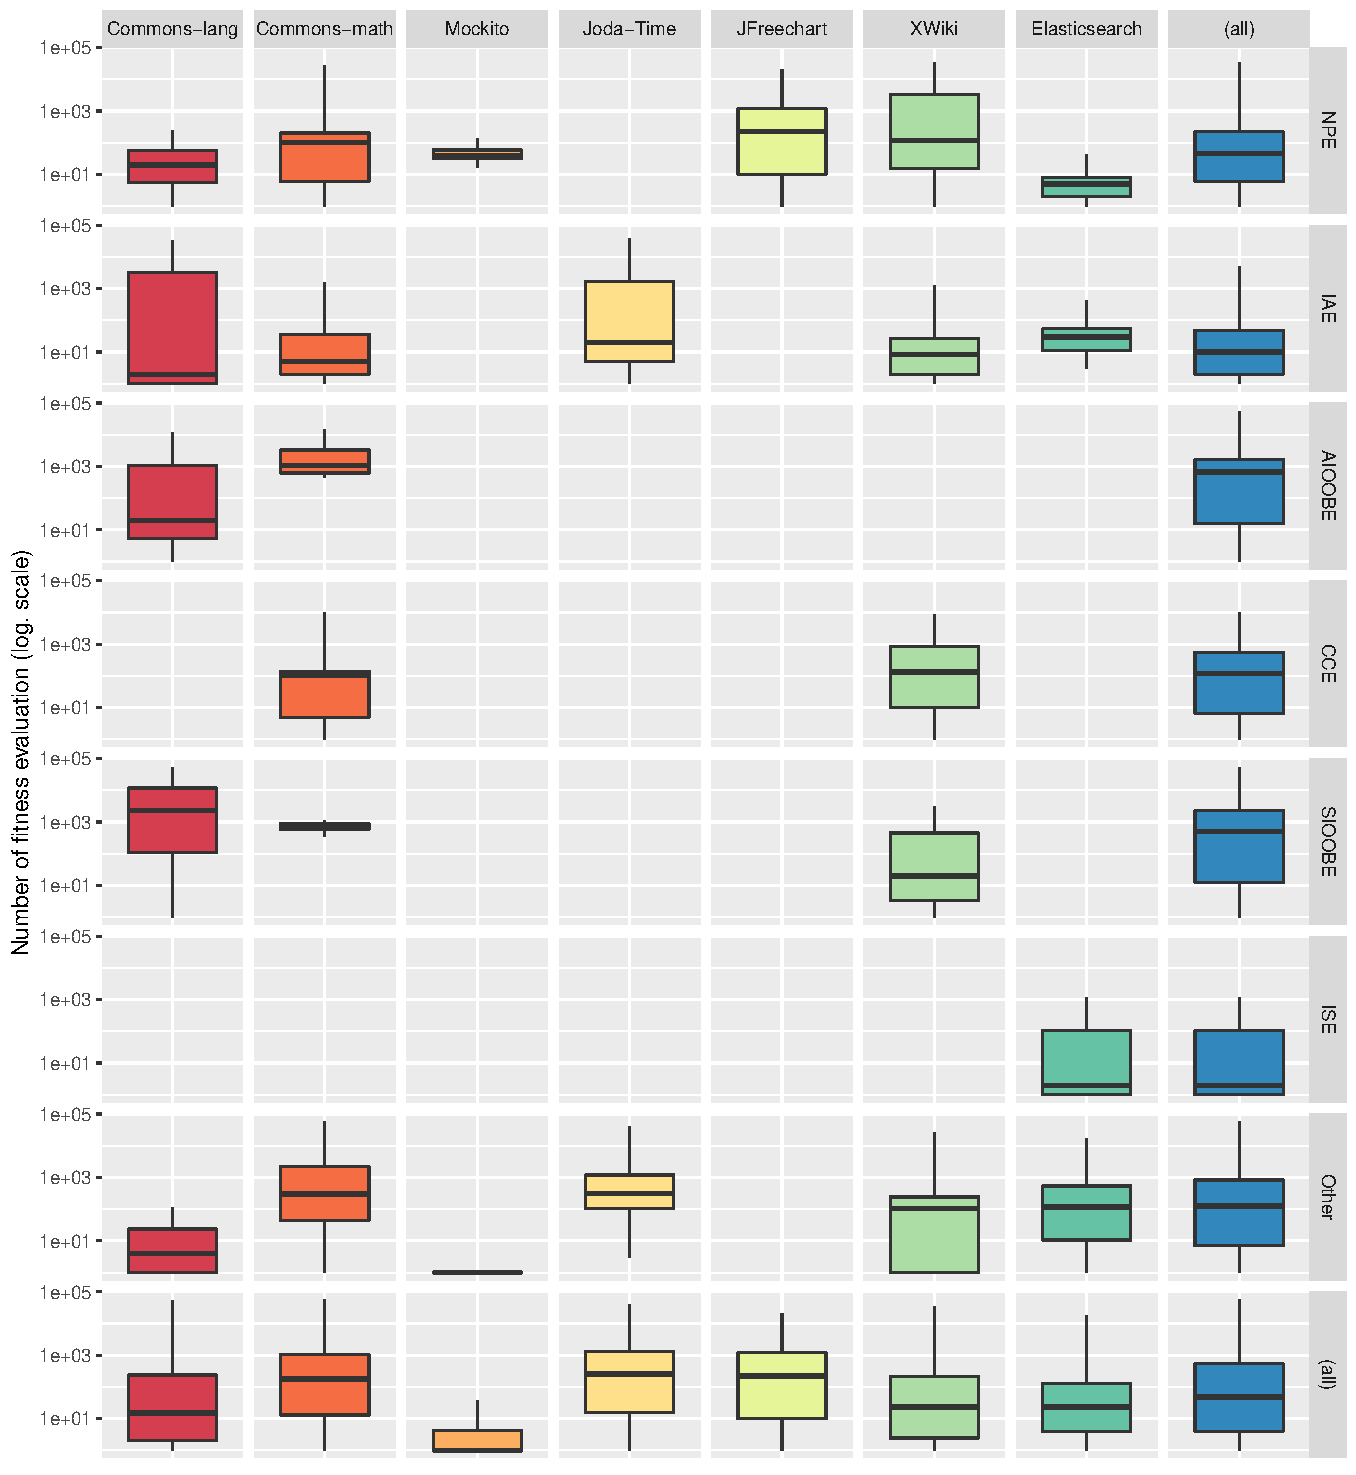
\includegraphics[width=\textwidth]{papers/jcrashpack/rq2_excepappstats.pdf}
	\caption{Average number of fitness evaluations for the \textit{reproduced} frames for each applications and exception type.}
	\label{figure:appexcepstats}
\end{figure*}

Considering the presented results in Figure~\ref{figure:outcomecomp} and Table~\ref{tab:appstats}, crash replication for various exceptions may be dependent on project type.
Figure~\ref{figure:appexcepstats} presents the results of crash reproduction grouped both by applications and exception types.
%
As the figure shows, the cost of reproducing NPE is lower for Elasticsearch, compared to XWiki and JFreechart, and the cost of reproducing IAE is lower for Commons-lang than for Elasticsearch.
We also observe differences in terms of costs of reproducing AIOOBE and SIOOBE for different projects.
%Our results suggest that further investigation in terms of possible correlations between application types and exception types are needed to be able to recommend a adequate number of fitness evaluations to \evocrash users when trying to reproduce a crash for a particular application.


\paragraph{\textbf{Summary (RQ$_{2.1}$)} How does project type influence performance of \evocrash for crash reproduction?}

%To summaries,  the median number of fitness evaluations required to reproduce a crash from Commons-lang, Mockito, XWiki, and Elasticsearch is low, compared to the median number of fitness evaluations needed to reproduce a crash from Commons-math, Joda-Time, and JFreechart. 

We observed that the factors are 
\begin{inparaenum}[(i)]
\item the complexity of the the project, and 
\item the level of the reproduced frames (reproducing higher frame requires more effort).
\end{inparaenum}
Furthermore, we see no link between the size of the project and the effort required to reproduce one of its crashes.


\paragraph{\textbf{Summary (RQ$_{2.2}$)} How does exception type influence performance of \evocrash for crash reproduction?}

For the exceptions, we observe that for ClassCastException, ArrayIndexOutOfBoundsException and StringIndexOutOfBoundsException, the cost of generating a crash-reproducing test case is high, while for NullPointerException, IllegalArgumentException, and IllegalStateException, the cost is lower.
This result indicates that the cost of reproducing types of exceptions for a non-trivial scenario (\textit{e.g.}, class conflicts or accessing an illegal state of an array) needs a more complex input generation. Furthermore, accessing the corresponding complex state is more time consuming for the search process.



\section{Challenges For Crash Reproduction (RQ3)}
\label{sec:jcrashpack:challenges}

\begin{table}[t]
    \centering
	\caption{Challenges with the number and percentage of frames identified for this challenge.}
	\label{tab:challenges}
	\begin{tabular}{l r r} 
\textbf{Category} & \textbf{Frames} & \textbf{Frequency}  
\\\hline 
Input Data Generation & 825 & 49.91\%\\ 
Abstract Class & 242 & 14.64\%\\ 
Anonymous Class & 142 & 8.59\%\\ 
Static Initialization & 141 & 8.53\%\\ 
Complex Code & 118 & 7.14\%\\ 
Private Inner Class & 56 & 3.39\%\\ 
Environmental Dependencies & 52 & 3.15\%\\ 
Irrelevant Frame & 37 & 2.24\%\\ 
Unknown Sources& 16 & 0.97\%\\ 
Nested calls & 10 & 0.60\%\\ 
try/catch & 7 & 0.42\%\\ 
Interface & 6 & 0.36\%\\ 
Empty Enum Type & 1 & 0.06\%\\ 
\hline 
\textbf{Total} & 1653 & 100\% \\ 
\end{tabular}
\end{table}

To identify open problems and future research directions, we manually analyzed the execution logs of 1,653 frames that could not be reproduced in any of the 10 executions.
This analysis includes a description of the reason why a frame could not be reproduced.\footnote{Available at \url{https://github.com/STAMP-project/EvoCrash-JCrashPack-application/tree/master/results/manual-analysis}.}
Based on those descriptions, we grouped the reason of the different failures into 13 categories and identified future research directions.
%This manual process took 9 person-weeks in total.
%
Table \ref{tab:challenges} provides the number and frequency of frames classified in each category.\footnote{For each category, we provide illustrative examples from \url{https://github.com/STAMP-project/EvoCrash-JCrashPack-application/tree/master/results/examples}.} The complete categorization table is available in our replication package.\footnote{The full table is available at \url{https://github.com/STAMP-project/EvoCrash-JCrashPack-application/blob/master/results/manual-analysis/categorisation.csv}.} 

%We divide the categories into two groups. The first group present categories previously identified in related search-based software testing literature. For each category of this group, we discuss how they impede search-based crash reproduction in particular. The second group presents newly identified categories and, for each category, discuss how they impact search-based crash reproduction, but also how they could affect search-based software testing in general. 

For each challenge, we discuss to what extent it is crash-reproduction-specific and its relation to search-based software testing in general. In particular, for challenges previously identified by the related literature in search-based test case generation, we highlight the differences originating from the crash reproduction context.
%\subsection{Challenges previously identified in search-based software testing}

%Seven of the thirteen challenges directly relate to challenges previously identified for search-based testing in general. We confirm their relevance and highlight the differences originating from the crash reproduction context.


\subsection{Input data generation}

Generating complex input objects is a challenge faced by many automated test generation approaches, including search-based software testing and symbolic execution \cite{braione2017tardis}.
Usually, the input space of each input is large and generating proper data enabling the search process to cover its goals is difficult.

As we can see from Table \ref{tab:challenges}, this challenge is substantial in search-based crash reproduction.
Trying to replicate a crash for a target frame requires to set the input arguments of the target method and all the other calls in the sequence properly such that when calling the target method, the crash happens.
Since the input space of a method is usually large, this can be challenging.
\evocrash uses randomly generated \emph{input arguments} and mock objects as inputs for the target method.
As we described in Section~\ref{sec:jcrashpack:evocrashevalresults}, we observe that a widespread problem when reproducing a \textit{ClassCastException} (CCE) is to identify which types to use as input parameters such that a CCE is thrown.
In the case of a CCE, this information can be obtained from the error message of the exception. Our future work includes harvesting additional information, like error messages, to help the search process. 

We also noticed that some stack traces involving Java \emph{generic types} make \evocrash abort the search after failing to inject the target method in every generated test during the guided initialization phase.
Generating \emph{generic type} parameters is also a recognized challenge for automated testing tools for Java \cite{fraser2014automated}.
To handle these parameters, \evocrash, based on \evosuite's implementation \cite{fraser2014automated}, collects candidate types from \texttt{castclass} and \texttt{in\-stance\-of} operators in Java bytecode, and randomly assign them to the type parameter.
Since the candidate types may themselves have generic type parameters, a threshold is used to avoid large recursive calls to generic types.
One possible explanation for the crashes in these cases could be that the threshold is not correctly tuned for the kind of classes involved in the recruited projects.
Thus, the tool fails to set up the target method to inject to the tests.
Based on the results of our evaluation, handling Java generics in \evocrash needs further investigation to identify the root cause(s) of the crashes and devise effective strategies to address them.

\begin{lstlisting}[frame=tb,
  caption={Excerpt of the stack trace for the crash XWIKI-13708},
  label=list:XWIKI13708,
  captionpos=t,
  numbers=left,
  float=t,
  firstnumber=0]
java.lang.NullPointerException: null
  at com.xpn.xwiki.internal.template.TemplateListener.onEvent(TemplateListener.java:79)
  at org.xwiki.observation.internal.DefaultObservationManager.notify(DefaultObservationManager.java:307)
  at org.xwiki.observation.internal.DefaultObservationManager.notify(DefaultObservationManager.java:269)
  [...]
\end{lstlisting}

\begin{lstlisting}[frame=tb,
  caption={Code excerpt from method \texttt{onEvent} in \texttt{TemplateListener.java}},
  label=list:input-generation:example,
  captionpos=t,
  language=Java,
  numbers=left,
  firstnumber=72,
  float=t,
  stepnumber=1]
public void onEvent(Event event, Object source, Object data) {
  XWikiDocument document = (XWikiDocument) source;

  if (document.getXObject(WikiSkinUtils.SKINCLASS_REFERENCE) != null) {
    if (event instanceof AbstractAttachmentEvent) {
      XWikiAttachment attachment = document.getAttachment(((AbstractAttachmentEvent) event).getName());
      String id = this.referenceSerializer.serialize(attachment.getReference()); // target line (*@\label{line:input-generation:target}@*)
      [...]
    }
  }
}
\end{lstlisting}

For instance, \evocrash cannot reproduce the first frame of crash XWIKI-13708\footnote{\url{https://jira.xwiki.org/browse/XWIKI-13708}}, presented in Listing \ref{list:XWIKI13708}. The target method \texttt{onEvent} (detailed in Listing \ref{list:input-generation:example}) has three parameters.
\evocrash could not reach the target line (line \ref{line:input-generation:target} in Listing \ref{list:input-generation:example}) as it failed to generate a fitted value for the second parameter (\texttt{source}). This (\texttt{Object}) parameter should be castable to \texttt{XWikiDocument} and should return values for \texttt{getXObject()} or \texttt{getAttachment()} (using mocking for instance).

\paragraph{Chosen examples:} 
XWIKI-13708, frame 1;
ES-22922, frame 5;
ES-20479, frame 10.\footnote{See \url{https://github.com/STAMP-project/EvoCrash-JCrashPack-application/blob/master/results/examples/InputDataGeneration.md}.}


\subsection{Complex code}

Generating tests for complex methods is hard for any search-based software testing tool \cite{MarkFlag}. In this study, we indicate a method as complex if 
\begin{inparaenum}[(i)]
\item it contains more than 100 lines of code and high cyclomatic complexity; 
\item it holds nested predicates ~\cite{GordonFlag, MarkFlag}; or
\item it has the \textit{flag problem}~\cite{GordonFlag,McMinn2011}, which include (at least one) branch predicate with a binary (boolean) value, making the landscape of the fitness function flat and turning the search into a random search \cite{MarkFlag}.
\end{inparaenum}

As presented in Section~\ref{sec:background:evocrash:guidedalg}, the first component of the fitness function that is used in \evocrash encodes how close the algorithm is to reach the line where the exception is thrown.
Therefore, frames of a given stack trace pointing to methods with a high code complexity\footnote{In some cases for Elasticsearch, the failing methods have nearly 300 lines of source code.} are more costly to reproduce, since reaching the target line is more difficult.  

Handling complex methods in search-based crash reproduction is harder than in general search-based testing. 
The search process in crash reproduction should cover (in most cases) only one specific path in the software under test to achieve the reproduction. 
If there is a complex method on this path, the search process cannot achieve reproduction without covering it. 
Unlike the more general coverage driven search-based testing approach (with line coverage for instance), where the are usually multiple possible executions paths to cover a goal.

\paragraph{Chosen examples:} 
XWIKI-13096, frame 3;
ES-22373, frame 10.\footnote{See \url{https://github.com/STAMP-project/EvoCrash-JCrashPack-application/blob/master/results/examples/ComplexCode.md}.}


\subsection{Environmental dependencies} 

As discussed by Arcuri et al.~\cite{Arcuri2014b}, generating unit tests for classes which interact with the environment leads to
\begin{inparaenum}[(i)]
\item difficulty in covering certain branches which depend on the state of the environment, and
\item generating flaky tests \cite{Luo2014}, which may sometimes pass, and sometimes fail, depending on the state of the environment. 
\end{inparaenum}
%
Despite the numerous advances made by the search-based testing community in handling environmental dependencies \cite{Arcuri2014b, Fraser2014b}, we noticed that having such dependencies in the target class hampers the search process.
%
Since \evocrash builds on top of \evosuite~\cite{fraser2012whole}, which is a search-based \textit{unit} test generation tool, we face the same problem in the crash reproduction problem as well.

\begin{lstlisting}[frame=tb,
float=t,
  caption=Stack trace for the crash XWIKI-12584,
  label=lst:XWIKI12584,
  captionpos=t,
  basicstyle={\scriptsize\ttfamily},
  numbers=left,
  firstnumber=0,
  breaklines=true,
  breakatwhitespace=true,
  tabsize=3,
  ]
java.lang.ClassCastException: [Ljava.lang.Object; cannot be cast to java.lang.String
  at [...].XWikiHibernateStore.searchDocumentReferencesInternal([...]:2457)
  at [...].XWikiHibernateStore.searchDocumentsNamesInternal([...]:2440)
  at [...].XWikiHibernateStore.searchDocumentsNames([...]:2246)
  at [...].XWikiHibernateStore.searchDocumentsNames([...]:2230)
  at [...].XWikiCacheStore.searchDocumentsNames([...]:373)
  at [...].XWiki.searchDocuments([...]:576)
\end{lstlisting}	

For instance, Listing~\ref{lst:XWIKI12584} shows the stack trace of the crash XWIKI-12584.\footnote{Reported at \url{https://jira.xwiki.org/browse/XWIKI-12584} and analyzed at \url{https://github.com/STAMP-project/EvoCrash-JCrashPack-application/blob/master/results/manual-analysis/Xwiki/XWIKI-12584.md}.} 
During the evaluation, \evocrash could not reproduce any of the frames of this stack trace. 
During our manual analysis, we discovered that, for the four first frames, \evocrash was unable to instantiate an object of class \texttt{XWikiHibernateStore},\footnote{See \url{https://github.com/xwiki/xwiki-platform/blob/xwiki-platform-7.2-milestone-2/xwiki-platform-core/xwiki-platform-oldcore/src/main/java/com/xpn/xwiki/store/XWikiHibernateStore.java}} resulting in an abortion of the search.
Since the class \texttt{XWikiHibernateStore} relies on a connection to an environmental dependency (here, a database), generating unit test requires substantial mocking code\footnote{See \url{https://github.com/xwiki/xwiki-platform/blob/xwiki-platform-7.2-milestone-2/xwiki-platform-core/xwiki-platform-oldcore/src/test/java/com/xpn/xwiki/store/XWikiHibernateStoreTest.java}} that is hard to generate for \evocrash. 
As for input data generation, our future work includes harvesting and leveraging additional information from existing tests to identify and use relevant mocking strategies. 

\paragraph{Chosen examples:} 
ES-21061, frame 4;
XWIKI-12584, frame 4.\footnote{See \url{https://github.com/STAMP-project/EvoCrash-JCrashPack-application/blob/master/results/examples/EnvironmentalDependencies.md}.}


\subsection{Static initialization}

In Java, static initializers are invoked only once when the class containing them is loaded.
As explained by Fraser and Arcuri~\cite{Fraser2014b}, these blocks may depend on static fields from other classes on the classpath that have not been initialized yet, and cause exceptions such as \texttt{NullPointerException} to be thrown.
In addition, they may involve environmental dependencies that are restricted by the security manager, which may also lead to unchecked exceptions being generated.

In our crash reproduction benchmark, we see that about 9\% (see Table \ref{tab:challenges}) of the cases cannot be reproduced as they point to classes that have static initializers.
When such frames are used for crash reproduction with \evocrash, the tool currently aborts the search without generating any crash reproducing test.
%
As Fraser and Arcuri~\cite{Fraser2014b} discuss, automatically determining and solving all possible kinds of dependencies in static initializers is a non-trivial task that warrants dedicated research.

\paragraph{Chosen examples:} 
ES-20045, frames 1 and 2.\footnote{See \url{https://github.com/STAMP-project/EvoCrash-JCrashPack-application/blob/master/results/examples/StaticInitialisation.md}.}


\subsection{Abstract classes and methods}
\label{sec:categoryabstractclasses}

In Java, abstract classes cannot be instantiated.
Although generating coverage driven unit tests for abstract classes is possible (one would most likely generate unit tests for concrete classes extending the abstract one or use a parametized test to check that all implementations respect the contract defined by the abstract class), when a class under test is abstract, \evosuite (as the general test generation tool for java) looks for classes on the classpath that extend the abstract class to create object instances of that class. 
In order to cover (e.g., using line coverage) specific parts of the abstract class, \evosuite needs to instantiate the right concrete class allowing to execute the different lines of the abstract class. 

For crash reproduction, as we can see from Table~\ref{tab:challenges}, it is not uncommon to see abstract classes and methods in a stack trace. 
In several cases from Elasticsearch, the majority of the frames from a given stack trace point to an abstract class.
Similarly to coverage-driven unit test generation, \evocrash needs to instantiate the right concrete class: if \evocrash picks the same class that has generated the stack trace in the first place, then it can generate a test for that class that reproduces the stack trace. 
However, if \evocrash picks a different class, it could still generate a test case that satisfies the first two conditions of the fitness function (section~\ref{sec:background:evocrash:guidedalg}). 
In this last case, the stack trace generated by the test would match the frames of the original stack trace, as the class names and line numbers would differ.
The fitness function would yield a value between 0 and 1, but it may never be equal to~0.

\paragraph{Chosen examples:} 
ES-22119, frames 3 and 4;
XRENDERING-422, frame 6.\footnote{See \url{https://github.com/STAMP-project/EvoCrash-JCrashPack-application/blob/master/results/examples/AbstractClass.md}.}


\subsection{Anonymous classes}

As discussed in the study by Fraser \etal~\cite{fraser2012whole}, generating automated tests for covering anonymous classes is more laborious because they are not directly accessible. 
We observed the same challenge during the manual analysis of crash reproduction results generated by \evocrash.
When the target frame from a given crash stack trace points to an anonymous object or a lambda expression, guided initialization in \evocrash fails, and \evocrash aborts the search without generating any test.

\paragraph{Chosen examples:} 
ES-21457, frame 8;
XWIKI-12855, frames 30 and 31.\footnote{See \url{https://github.com/STAMP-project/EvoCrash-JCrashPack-application/blob/master/results/examples/AnonymousClass.md}.}


\subsection{Private inner classes}

Since it is not possible to access a private inner class, and therefore, not possible to directly instantiate it, it is difficult for any test generation tool in Java to create an object of this class.
As for anonymous classes, this challenge is also present for crash reproduction approaches.
In some crashes, the target frame points to a failing method inside a private inner class.
Therefore, it is not possible to directly inject the failing method from this class during the guided initialization phase, and \evocrash aborts the search.

\paragraph{Chosen example:} 
MATH-58b, frame 3.\footnote{See \url{https://github.com/STAMP-project/EvoCrash-JCrashPack-application/blob/master/results/examples/PrivateInnerClass.md}.}


%\subsection{Crash reproduction related challenges}

%We identified six new challenges (out of thirteen). For each one, we also describe how it can affect search-based software testing in general. 


\subsection{Interfaces}

In 6 cases, the target frame points to an interface.
In Java, similar to abstract classes, interfaces may not be directly instantiated.
In these cases also, \evocrash randomly selects the classes on the classpath that implement the interface and, depending on the class picked by \evocrash, the fitness function may  not reach $0.0$ during the search if the class is different from the one used when the input stack trace has been generated.
%
This category is a special case of \emph{Abstract classes and methods} (described in Section \ref{sec:categoryabstractclasses}), however, since the definition of a default behavior for an interface is a feature introduced by Java~8 \cite{jdk8release} that has, to the best of our knowledge, not been previously discussed for search-based testing, we choose to keep it as a separate category. 

\paragraph{Chosen example:}
ES-21457, frame 9.\footnote{See \url{https://github.com/STAMP-project/EvoCrash-JCrashPack-application/blob/master/results/examples/Interface.md}.}


\subsection{Nested private calls}

In multiple cases, the target frame points to a private method. As we mentioned in Section \ref{sec:jcrashpack:evocrashevalsetup}, those private methods are not directly accessible by \evocrash. 
To reach them, \evocrash detects other public or protected methods which invoke the target method directly or indirectly and randomly choose during the search. 
If the chain of method calls, from the public caller to the target method, is too long, the likelihood that \evocrash may fail to pick the right method during the search increases.

In general, calling private methods is challenging for any automated test generation approach.
For instance, Arcuri \etal \cite{arcuri2017private} address this problem by using the Java reflection mechanism to access private methods and private attributes during the search. 
As mentioned in Section \ref{se:evalsetup}, this can generate invalid objects (with respect to their class invariants) and lead to generating test cases helplessly trying to reproduce a given crash \cite{Chen2015}.

\paragraph{Chosen examples:} 
XRENDERING-422, frames 7 to 9.\footnote{See \url{https://github.com/STAMP-project/EvoCrash-JCrashPack-application/blob/master/results/examples/NestedPrivateCalls.md}.}


\subsection{Empty \texttt{enum} type}

In the stack trace of the ES-25849 crash,\footnote{The analysis is available at \url{https://github.com/STAMP-project/EvoCrash-JCrashPack-application/blob/master/results/manual-analysis/Elasticsearch/ES-25849.md}.} 
the 4th frame points to an empty enumeration Java type.\footnote{See \url{https://github.com/jimczi/elasticsearch/blob/0a4b38b60c2752cdc6de819f5bf3414bd01f88c5/core/src/main/java/org/elasticsearch/index/fielddata/ordinals/GlobalOrdinalsBuilder.java}.} 
Since there are no values in the enumeration, \evocrash was not able to instantiate a value and \emph{aborted} during the initialization of the population.
Frames pointing to code in an empty enumeration Java type should not be selected as target frames and could be filtered out using a preliminary static analysis.

\paragraph{Chosen example:} 
ES-25849, frame 4.

\subsection{Frames with \texttt{try}/\texttt{catch}}

Some frames have a line number that designates a call inside a \texttt{try/catch} block.
When the exception is caught, it is no longer thrown at the specific line given in the trace, rather it is typically handled inside the associated \texttt{catch} blocks.
From what we observed, often catch blocks either
\begin{inparaenum}[(i)]
\item re-throw a checked exception, which yield chained stack traces with information that is not exactly as the input stack trace but can still be used for crash reproduction;
 or \item log the caught exception.
\end{inparaenum}
%
Since \evocrash only considers uncaught exceptions that are generated as the result of running the generated test cases during the search, the logged stack traces is presently no use for crash reproduction. Also, even if a stack trace is recorded to an error log, this stack trace is not the manifestation of a crash \textit{per se}. Indeed, once the exception logged, the execution of the program continues normally. 

For instance, for the crash ES-20298,\footnote{Reported at \url{https://github.com/elastic/elasticsearch/issues/20298} and analyzed at \url{https://github.com/STAMP-project/EvoCrash-JCrashPack-application/blob/master/results/manual-analysis/Elasticsearch/ES-20298.md}} \evocrash cannot reproduce the fourth frame of the crash. This frame points to the following method call in a \texttt{try} and \texttt{catch}:
%
\begin{lstlisting}[language=Java]
try {
    processResponse(response);
} catch (Throwable t) {
    onFailure(t);
}
\end{lstlisting}
%
Even if an exception is thrown by the \texttt{processResponse} method, this exception is caught and logged, and the execution of the program continues normally. 

Generally, if an exception is caught in one frame, it cannot be reproduced (as it cannot be observed) from higher level frames. For instance, for ES-20298, all frames above level 4 cannot be reproduced since the exception is catch in frame 4 and not propagated to the higher frames. 
This property of a crash stack trace implies that, for now, depending on where in the trace such frames exist, only a fraction of the input stack traces can actually be used for automated crash reproduction.
Future development of \evocrash can alleviate this limitation by, additionally to the monitoring of uncaught exceptions, read the error log to affecting the propagation of exceptions during execution. 
However, unlike other branching instructions relying on boolean values, for which classical coverage driven unit test generation can use the \emph{branch distance} (see Section \ref{sec:background:evocrash:guidedalg}) to guide the search \cite{McMinn2004}, there is little guidance offered for \texttt{try/catch} instructions since the branching condition is implicit in one or more instructions in the \texttt{try}. 

\paragraph{Chosen example:} 
ES-14457, frame 4.\footnote{See \url{https://github.com/STAMP-project/EvoCrash-JCrashPack-application/blob/master/results/examples/TryCatch.md}.}


\subsection{Missing line number}

\begin{lstlisting}[frame=tb,
  float=t,
  caption=An excerpt of the stack trace from the crash XRENDERING-422  with missing line numbers,
  label=list:missing,
  captionpos=t,
  basicstyle={\scriptsize\ttfamily},
  numbers=left,
  breaklines=true,
  breakatwhitespace=false,
  tabsize=3]
at org.apache.xerces.parsers.XMLParser.parse(Unknown Source)
at org.apache.xerces.parsers.AbstractSAXParser.parse(Unknown Source)
at org.xml.sax.helpers.XMLFilterImpl.parse(XMLFilterImpl.java:357)
\end{lstlisting}

31 frames in \crashpack have frames with a missing line number, as shown in Listing~\ref{list:missing}.
This happens if the Java files have been compiled without any \emph{debug} information (by default, the Java compiler add information about the source files and line numbers, for instance, when printing a stack trace) or if the frame points to a class part of the standard Java library and the program has been run in the Java Runtime Environment (JRE) and not the JDK.

Since \evocrash currently requires a line number to compute the fitness values during the search, those frames have been ignored during our evaluation and do not appear in the results.
Yet, as frames with missing line number appear in \crashpack (and in other stack traces), we decided to mention this trial here as a search-based crash reproduction challenge.
A possible solution, as the future work, is to relax the fitness function so that it can still approximate fitness if line numbers are missing.

\paragraph{Chosen example:} 
XRENDERING-422.\footnote{The stack trace is available at \url{https://github.com/STAMP-project/EvoCrash-JCrashPack-application/blob/master/evaluation/JarFiles/resources/logs/XWIKI/XRENDERING-422/XRENDERING-422.log}}


\subsection{Incorrect line numbers}

In 37 cases, the target frame points to the line in the source code where the target class or method is defined.
This happens when the previous frame points to an anonymous class or a lambda expression.
Such frames practically cannot be used for crash reproduction as the location they point to does not reveal where exactly the target exception occurs.
One possible solution would be to consider the frame as having a missing line number and use the relaxed fitness function to approximate the fitness. 

\paragraph{Chosen examples:} 
MATH-49b, frames 1 and 4.\footnote{See \url{https://github.com/STAMP-project/EvoCrash-JCrashPack-application/blob/master/results/examples/IrrelevantFrames.md}.}


\subsection{Unknown}

We were unable to identify why \evocrash failed to reproduce 16 frames (out of 1,653 frames manually analyzed). 
In these cases, neither the logs nor the source code could help us understand how the exception was propagated. 
%Therefore, factor which leads \evocrash to fail to reproduce the crash could not be clearly identified.


\paragraph{\textbf{Summary (RQ$_3$)} What are the open problems that need to be solved to enhance search-based crash reproduction?}

Based on the manual analysis of the frames that could not be reproduced at least once out of 10 rounds of executions, we identified 13 challenges for search-based crash reproduction.
We confirmed challenges previously identified in other search-based software testing approaches and specified how they affect search-based crash reproduction. And discovered new challenges, more specific to search-based crash reproduction and explained how the can affect other search-based software testing approaches. 

These challenges are related to the difficulty to generate test cases due to complex input data, environmental dependencies, or complex code; abstraction (static initialization, interfaces, abstract, and anonymous classes); encapsulation mechanisms (private inner classes and nested private calls in the given stack trace) of object-oriented languages; or the selection of the target frame in crash reproduction (in \texttt{try}/\texttt{catch} blocks, in empty enumerations, when the location in the source code is unknown, or when the frame has an incorrect line number).


\section{Discussion}
\label{sec:jcrashpack:discussion}

\subsection{Empirical evaluation for crash reproduction}

Conducting empirical evaluation for crash reproduction is challenging. It requires to collect various artifacts from different sources and to analyze the results to determine, in the case of a negative outcome, the cause that prevents the crash reproduction. Some are easy to fix, like missing dependencies that were added to the project linked to the stack trace, and for which we rerun the evaluation on the stack traces. The others are detailed in Section \ref{sec:jcrashpack:challenges}, and serve to identify future research directions. 

One of the most surprising causes is due to a line mismatch in some stack traces.
During the manual analysis of our results, we found out that three frames in two different stack traces, coming from Defects4J projects, target the wrong lines in the source code: the line numbers in the stack traces point to lines in the source code that cannot throw the targeted exception.
Since the stack traces were collected directly from the Defects4J data (which reports failing tests and their outputs), we tried to regenerate them using the provided test suite and found a mismatch between the line numbers of the stack traces indeed.
We reported those two projects to the Defects4J developers:\footnote{See the issue at \url{https://github.com/rjust/defects4j/issues/142}.} a bug in JDK7~\cite{JDK7024096} causes this mismatch.
Since \evocrash relies on line numbers to guide its search, it could not reproduce the crashes.
We recompiled the source code, updated the stack trace accordingly in \crashpack, and rerun the evaluation for those two stack traces.

Thanks to \crashpack and \exrunner, we are now able to ease empirical evaluation for crash reproduction. \exrunner can be extended to other crash reproduction tools\footnote{See how to extend \exrunner at \url{https://github.com/STAMP-project/ExRunner}.} for comparison, or assess the development of new ideas in existing tools. Our future work also includes the prioritization of crashes from \crashpack to allow quick feedback on new ideas in a fast and automated way~\cite{Alshahwan2018}.


\subsection{Usefulness for debugging}


In our evaluation, we focused on the crash-replication capabilities of \evocrash and identified problems affecting those capabilities. 
We considered the generated tests only to classify the outcomes of the \evocrash generation process but did not assess their actual usefulness for debugging. 

Chen \etal \cite{Chen2015} introduced a usefulness criterion for the crash reproduction approaches. 
According to this criterion, a crash reproducing test is useful to the developers if it covers the buggy frame: i.e., if the target frame for which the reproduction is successful is higher than the frame that points to the buggy method.

In our previous work \cite{Soltani2018a}, we conducted a controlled experiment to assess the usefulness of \evocrash for debugging and bug fixing of two crashes (one from Apache Commons Collections and one from Apache Log4j) with 35 master students. Results show that using a crash-replicating test case generated by \evocrash may help to locate and fix the defects faster. Also, this study confirmed the usefulness criterion defined by the Chen \etal \cite{Chen2015} but also found evidence that test cases categorized as not useful can still help developers to fix the bug. 

Since \crashpack also includes two open source industrial and actively maintained applications, it represents an excellent opportunity to confirm the usefulness of \evocrash in an industrial setting. 
The key idea is to centralize the information in the issue tracker by providing a test case able to replicate the crash reported in an issue in the same issue (as an attachment for instance).
This can be automated using, for instance, a GitHub, GitLab or JIRA plugin that executes \evocrash when a new issue contains a stack trace.
To assess the usefulness of \evocrash in an industrial setting, we plan to setup a case study \cite{Wohlin2012} with our industrial partners. 
Hereafter, we outline the main steps of the evaluation protocol using XWiki as subject: 
\begin{inparaenum}[(i)]
\item select four crashes to fix (two from open issues and two from closed issues) for which \evocrash could generate a crash reproducing test for frame 3 or higher;
\item clone the XWiki Git repository in GitHub and open four issues, corresponding to the four crash;
\item remove the fix for the two fixed issues;
\item for each issue, append the test case generated by \evocrash; \label{item:addtestcases}
\item ask (non-XWiki) developers to fix the issues;
and finally, \item repeat the same steps without adding the test cases generated by \evocrash (i.e., omit step \ref{item:addtestcases}).
\end{inparaenum}
%
We would measure the time required to fix the issues (by asking participants to log that time). For the two previously fixed issues, we will compare the fixes provided by the participants with the fixes provided by XWiki developers. And for the two open issues, we will ask feedback from the XWiki developers through a pull request with the different solutions. 

%However, this evaluation is not trivial and requires a significant effort to either control and observe the environment of the developer when asked to perform a debugging task. 
%Or, to analyze and compare the generated crash-reproducing test with the messages in the issue tracker and the code fix in the code version system, with additional threats to the validity linked to the interpretation of the notes in the issue tracker and of the code fix. 

\subsection{Benchmark building}

\crashpack is the first benchmark dedicated to crash reproduction.
We deliberately made a biased selection when choosing Elasticsearch as the most popular, trending, and frequently-forked project from GitHub.
Elasticsearch was among several other highly ranked projects, which addressed other application domains, and thus were interesting to explore.
In the future, further effort should extend \crashpack, possibly by:
\begin{inparaenum}[(i)]
\item using a \textit{random selection} methodology for choosing projects; 
\item involving industrial projects from other application domains;
and \item automatically collecting additional information about the crashes, the stack traces, and the frames to further understand current strengths and limitations of crash reproduction.
\end{inparaenum}

Building \crashpack required substantial manual effort, not just for finding the issues, but also for collecting the right versions of the system itself and its dependencies needed  to reproduce the given crash.
Since we want it to be representative of current crashes, we need to automate this effort as much as possible: for instance, by mining stack traces from issue tracking systems \cite{Nayrolles2016}.

Despite the benefits that the evaluation infrastructure could get from the inclusion of \crashpack bugs in Defects4J, i.e., the isolation of the bugs to ease replicatbility of the evaluations \cite{just2014defects4j}, we designed \crashpack as a standalone instead of extending Defects4J.
The main reason is that not all bugs in Defects4J manifest as crashes (only 73 out of 395 where selected to be part of \crashpack). 
We also believe that the integration of the two benchmarks is not a smooth and easy process.
Defects4J requires isolation of the buggy and fixed versions of the source code, as wel as a test case able to expose the bug \cite{just2014defects4j}. However, not all issues were fixed at the time we collected the crashes in \crashpack.
Also, XWiki and Elasticsearch are much larger applications (124,000 NCSS for Elasticsearch, 177,000 NCSS for XWiki distributed in a hierarchy of several thousands of Maven projects) compared to the API libraries considered in Defects4J (63,000 NCSS for JFreeChart). 
Only building them with their default test suites already raised several issues. 
For those reasons, isolating the bug, the patch, and the non-regression test cases for such kind of large projects is not a trivial task. 









\section{Future Research Directions For Search-Based Crash Reproduction}
\label{sec:jcrashpack:futurework}

From the evaluation and the challenges derived from our manual analysis, we devise the following future research directions. 
While the same challenge can be addressed in different ways, some requiring technical improvements of \evocrash and other raising new research directions, we focus the discussion of this section on the latter. 

\subsection{Context matters}

While search-based crash-reproduction with \evocrash~\cite{soltani2017,Soltani2018a} outperformed other approaches based on \begin{inparaenum}[(i)]
\item backward symbolic execution \cite{Chen2015},
\item test case mutation \cite{Xuan2015},
and \item model-checking \cite{Nayrolles2017},
\end{inparaenum}
our evaluation shows that the extent to which crashes are reproduced varies.
These results indicate the need for taking various types of contexts and properties of software applications into account when devising an approach to a problem.
Thus, we show that indeed, rather than seeking a universal approach to search-based crash reproduction, it is important to find out and address challenges specific to various types of application domains (e.g., RESTful microservices vs. enterprise wiki applications)\cite{Arcuri2017b}.

Furthermore, search-based crash replication boils down to seeking the execution path that will reproduce a given stack trace.
As with other search-based testing approaches, it faces challenges about \emph{input data generation} during the search when the input space is large.
Previous research on \textit{mocking} and \textit{seeding} \cite{arcuri2017private,Rojas2016} address this problem by using functional mocking and extracting objects and constants from the bytecode.

We believe that \emph{taking context into account} should go one step further for crash replication.
With the development of DevOps \cite{Roche2013} and continuous integration and delivery pipelines, there is an increasing amount of available data on the execution of the software.
Those data can be used to guide the search more accurately.
For instance, by seeding the search using values observed in the execution logs and setting up values for \emph{environmental dependencies} (databases, external services, etc.).


\subsection{Stack trace preprocessing and target frame selection}

Various factors may influence the selection of a target frame in a stack trace.
As observed in our evaluation, when not performed cautiously, this selection leads to unsuccessful executions of \evocrash.
For instance, frames targeting code in a \emph{private inner class}, or \emph{irrelevant} source code location (like, as we observed, class header or annotation) should be discarded before performing the selection.

Frames targeting code in \emph{abstract classes} or \emph{interfaces} (only if the target method is defined in the interface, which is possible from Java 8) may be of some use to find the cause of the crash:  for instance, to identify an incorrect subclass implementation \cite{Liskov2000}.
However, as abstract classes and interfaces cannot be directly instantiated, the stack trace generated by \evocrash can never be exactly the same as the given stack trace.
And, as for \emph{input arguments} and \emph{generic type parameters}, \evocrash has no indication on which subclass to pick, making the search difficult.
In this case, considering higher level frames (i.e., frames that are lower in the stack trace) may help to pick the right subclass.

Those reasons motivate the need to develop \emph{stack trace analysis techniques} in order to help the \emph{selection} of a target frame.
This analysis will discard irrelevant and unknown source location frames and provide a visualization to the developer to have a clear view on what are his or her options, for instance by marking stack traces that point to interfaces and abstract classes and recommend him to pick higher level frames.

For a given stack trace, this analysis will also identify frames pointing to a \emph{try/catch} block.
Those stack traces are commonly reported by users to issue tracking systems but cannot (for now) be completely reproduced by \evocrash.
Further investigation on current error handling practices in Java code \cite{Cabral2007,Coelho2017} and how they are reported by users \cite{Maiga2015} will help us to devise efficient approaches to replicate such stack traces.

\subsection{Guided search}

Besides usage of contextual information to enhance the generation of test cases during the search process, we also consider to enhance the guidance itself.
Search based testing algorithms have several parameters (365 in \evocrash), like population size, search budget, probability of applying crossover and mutation, etc. 
As demonstrated by Arcuri and Fraser \cite{Arcuri2011a}, default parameters values work well on average, but may be fare from optimal for specific frames and stack traces. 
A better characterization of the stack traces in \crashpack, trying different \emph{parameters}, as well as improving the \emph{fitness function} itself are part of our future work.
For instance the fitness function could take other elements into account (e.g., compute a similarity for exception messages).
We will also consider multi-objectives search, where, for a given target frame, reproducing each lower  frame becomes an objective of the search.
We plan to reuse our evaluation infrastructure to compare those different approaches and investigate their different fitness landscapes to gain deeper understanding of the search process for crash reproduction. And eventually devise guidelines on \evocrash settings to maximize crash reproduction for a given stack trace and its characteristics.

\subsection{Improving testability}

Finally, as we observed, code complexity was among the major challenges in crash reproduction with \evocrash.
To improve testability, several testability transformation techniques \cite{McMinn2011, LiBytecodeTT, MarkFlag,MarkFlagRemoval, MarkLoopFlag} have been proposed in the literature so far.
Future research may investigate testability transformation techniques and their impact on search-based crash reproduction.


\section{Threats To Validity}
\label{sec:jcrashpack:threats}
% Threats to Validity

Evaluations of crash reproduction approaches, such as the one we conducted for \evocrash, come with threats to internal validity, external validity, and reliability.
The overarching goal of \crashpack is to reduce such threats for all evaluations of any crash reproduction tool, by offering a curated set of crashes to conduct such evaluations.

Concerning \emph{external validity}, we carefully designed \crashpack so that it offers a mix of small and large systems, as well as of different types of exceptions. Furthermore, it includes open source systems directly developed by industry.
%
Nevertheless, any set is incomplete, which is why we keep \crashpack open for extension, as discussed in Section~\ref{sec:jcrashpack:discussion}.  For example, there still remain several other domains, such as gaming or financial applications, for which there is no representative project in the benchmark. 

With respect to \emph{internal validity}, implementation faults can be a source of confounding factors. These can occur in the tools themselves, such as \evocrash or \evosuite, but also in the infrastructure used to actually conduct the experiment. To address the latter, \crashpack comes with \exrunner, which automates the process of scheduling, executing, monitoring, and reporting crash reproduction attempts.

Concerning \emph{reliability}, \crashpack and \exrunner make it easy to repeat experiments, thus making it possible for researchers to independently replicate each others crash reproduction findings.

Besides these threats partially mitigated by \crashpack, our evaluation of \evocrash comes with additional threats to (internal and external) validity. This particularly relates to the randomized nature of genetic algorithms, which we addressed by running the evaluations 10 times, and following the guidelines by Arcuri and Briand \cite{Arcuri2014} for analyzing the results. 
%
Furthermore, such threats concern the risk of bias during the manual analysis, which we mitigated by using cross-checking: the result of each manual analysis has been validated by at least one other person. 
In case of disagreement, we asked for a third opinion.
%
Finally, our evaluation includes only one tool: \evocrash. Previous work showed that \evocrash performs better than other state-of-the-art crash reproduction tools. 
Unfortunately, since to the best of our knowledge, no other tool was publicly available, we were not able to confirm that conclusion on the crashes in \crashpack. 
We believe that \crashpack enhances the current state-of-the-practice in crash reproduction research by offering a publicly available benchmark for which other tool providers can report their results. 




\section{Conclusion}
\label{sec:jcrashpack:conclusion}
Experimental evaluation of crash reproduction research is challenging, due to the computational resources needed by reproduction tools, the difficulty of finding suitable real life crashes, and the intricacies of executing a complex system so that the crash can be reproduced at all.

To remedy this problem, this chapter sets out to create a benchmark of Java crashes, that can be reused for experimental purposes.
To that end we propose \crashpack and \exrunner, a curated benchmark of 200 real life crashes, and a tool to conduct massive experiments on these crashes.
This benchmark is publicly available and can be used to compare existing and new tools against each other, as well as to analyze how proposed improvements to existing reproduction techniques actually constitute an improvement.

We applied the state of the art search-based Java crash reproduction tool, \evocrash, to \crashpack. Our findings include that the state of the art can reproduce 87 crashes out of 200 in a majority of time, that crash reproduction for industry-strength systems is substantially harder, and that \texttt{NullPointerException}s are generally easiest to reproduce. Furthermore, we identified 13 challenges that crash reproduction research needs to address to strengthen uptake in practice, as well a future research directions to address those challenges.

\crashpack  can be extended in various ways: by including more crashes from other types of applications; by automating the collection of information about the crashes and stack traces to further understand current strengths and limitations of crash reproduction; as well as automating the collection of the crashes themselves. Furthermore, since executing crash reproduction tools on 200 crashes may be time taking, \crashpack could be extended to offer prioritization for benchmarks, based on the known theoretical strengths and limitations if the tools. For instance, by ordering crashes based on the cyclomatic complexity of the involved frames to evaluate search-based or symbolic execution-based crash reproduction approaches. 

Finally, our future work for \evocrash itself include improving input data generation by taking information from the execution context and the application (e.g., existing source code and test cases) into account. We also want to deeper our understanding of stack traces in order to be able to recommend target frames to the developers. Finally, we will improve the search process itself by refining the fitness function to improve the guidance through the different frames of the stack trace.


\chapter{Search-based Crash Reproduction using Behavioral Model Seeding}
%%%%%%%%%%%%%%%%%%%%%%
\label{sec:model_seeding}
%%%%%%%%%%%%%%%%%%%%%%


% !TEX root =  ../STVR-model-seeding.tex



% The starting point of any debugging activity is to try to reproduce the problem reported by a user in the development environment~\cite{Zeller2009,BellerICSE2018}. In particular, for Java programs, when a crash occurs, an exception is thrown. A developer strives to reproduce it to understand its cause, then fix the bug, and finally add a (non-)regression test to avoid reintroducing the bug in future versions. 

% Manual crash reproduction can be a challenging and labor-intensive task for developers: it is often an iterative process that requires setting the debugging environment in a similar enough state as the environment in which the crash occurred~\cite{Zeller2009}. Moreover, it requires the developer to have knowledge of the system's components involved in the crash. 
%
%To help developers in their task, several automated crash reproduction methods, relying on different techniques, have been proposed: symbolic execution~\cite{Chen2015}, model checking~\cite{nayrolles2015jcharming,Nayrolles2017}, mutation testing~\cite{Xuan2015}, or evolutionary algorithms~\cite{BPT17concrash,soltani2017,Soltani2018b}.
%
% To help developers in their task, several automated crash reproduction methods, relying on different techniques, have been proposed \cite{Chen2015, nayrolles2015jcharming, Nayrolles2017, Xuan2015, BPT17concrash, soltani2017, Soltani2018b}.

% One of the most promising approaches is to generate crash-reproducing test cases using search-based software testing \cite{soltani2017, Soltani2018b}. This approach benefits from a \textit{guided genetic algorithm} which searches for the crash reproducing test case. Soltani \etal performed an empirical evaluation of \evocrash and reported that it outperforms other crash reproduction approaches~\cite{soltani2017}.

As confirmed by Chapter \ref{sec:jcrashpack:introduction}, one of the challenges of search-based crash reproduction is to bring enough information into the test generation process.
For instance, complex elements (like strings with a particular format or objects with a complex structure) are hard to initialize without additional information. 
This can lead to two different issues: first, complex elements take more time to be generated, which can prevent finding a solution within the time budget allocated to the search; and second, elements that require complex initialization procedures (\eg specific sequences of method calls to set up an object) may prevent starting the search if the search-based approach is unable to create an initial population. 

%In their recent work, Soltani \etal \cite{soltani2017, Soltani2018b} define \botsing, a search-based crash reproduction tool that uses a guided genetic algorithm to generate a test case able to replicate the crash. Soltani \etal performed an empirical evaluation of \botsing and reported that it outperforms other approaches~\cite{soltani2017}. However, as other search-based testing approaches, \botsing has limitations regarding its efficiency and applicability~\cite{Rojas2016}. For instance, complex elements (like strings with a particular format or objects with a complex structure) are hard to initialize without additional information. 
%This can lead to two different issues: first, complex elements increase the size of the search space, which can prevent to find a solution, event with a large time budget; and second, complex elements that require complex initialization procedures (\eg specific sequences of method calls to setup an object) may prevent the search to start if the search-based approach is unable to create an initial population. 

Rojas \etal~\cite{Rojas2016} demonstrated that \emph{seeding} is beneficial for search-based unit test generation. More specifically, by analyzing source code (collecting information that relates to numeric values, string values, and class types) and existing tests (collecting information about the behavior of the objects in the test) and making them available for the search process, the overall coverage of the generated test improves. 
%They applied seeding to \evosuite~\cite{Rojas2016} and confirmed that a good seeding strategy can lead to an overall improvement of the search results.
However, current seeding strategies focus on collecting and reusing values and object states as-is. 

In this paper, we define, implement, and evaluate a new seeding strategy, called \emph{behavioral model seeding}, which abstracts behavior observed in the source code and test cases using transition systems. The transition systems represent the (observed) usages of the classes and are used during the search to generate objects and sequences of method calls on those objects.

\emph{Behavioral model seeding} takes advantage of the advances made by the model-based testing community~\cite{Utting2007} and uses them to enhance search-based software testing. This seeding strategy helps the search process: 
\begin{inparaenum}[(i)]
\item it provides the possibility of covering the given crash by collecting information from various resources (\eg source code and existing test cases)  to infer a unique transition system; and
\item it finds the most beneficial seeding candidates, for guiding the crash reproduction search process, by defining a rational procedure for the selection of abstract object behaviors from the inferred models.
\end{inparaenum} 

%Since \botsing is based on \evosuite, it uses the default configuration for seeding and enables analysis of the source code for constants seeding, dynamic seeding, and type seeding. Other seeding strategies that use existing tests are not used by default and have never been evaluated on \botsing. 
%%
%In contrast to \evosuite that aims at generating a test suite that maximizes statement and branch coverage, the goal of \botsing is to generate a single test that replicates a crash. In this context, existing tests can be useful to focus the search as the execution steps leading to a crash are likely to be close to the execution steps of valid executions of the system.
%
%Currently, \botsing randomly generates test cases to initialize its search process. In this paper, we explore existing \emph{test seeding} strategies to adapt and evaluate them for crash reproduction, and devise a new \emph{model seeding} strategy subsuming test seeding and based on both static analysis of the source code and the dynamic execution of the existing test cases. Models are automatically generated using 2-grams \cite{Sprenkle2013,Tonella2014,Verwer2017} to abstract and generalize the behavior (compare to test seeding) of the system, and used to generate sequences of execution steps that are reused during the search.

We also adapt \emph{test seeding}, introduced by Rojas \etal, for search-based crash reproduction. Contrarily to model seeding, \emph{test seeding} relies only on the states of the objects observed during the execution of the test to seed a search process. Unlike search-based unit test generation, search-based crash reproduction does not seek to maximize the coverage of the class, but rather generates a specific test case able to reproduce a crash. Since test seeding has only been applied to search-based unit test generation~\cite{Rojas2016}, we first evaluate the use of test seeding for crash reproduction.  We then compare the results of test seeding with the application of \emph{model seeding}, which combines information on the objects states coming from the test cases with information collected in the source code, to search-based crash reproduction. 

We performed an evaluation on 122 crashes from 6 open-source applications to answer the following research questions: 
%
\begin{itemize}
\item[\textbf{RQ1}] What is the influence of \emph{test seeding used during initialization} on search-based crash reproduction?
\item[\textbf{RQ2}]  What is the influence of \emph{behavioral model seeding used during initialization}  on search-based crash reproduction?
\end{itemize}
%
We consider both research questions from the perspective of \emph{effectiveness} (of initializing the population and reproducing crashes) and \emph{efficiency}. We also investigate the factors (\eg the cost of analyzing existing tests) that influence the test and model seeding approaches and gain a better insight into how search-based crash reproduction works and how it can be improved.
Generally, our results indicate that behavioral model seeding increases the number of crashes that we can reproduce. 
More specifically, because of the randomness in the test generation process, we execute the crash replication multiple times and we observe that in the majority of these executions 4 crashes (out of 122) can be replicated; also, this seeding strategy can reproduce 9 crashes, which are not reproducible at all with no seeding, in at least one execution. In addition, this seeding strategy slightly improves the efficiency of the crash reproduction process. Moreover, model seeding enables the search process to start for three additional crashes. In contrast, using test seeding in crash-reproduction leads to a lower crash-reproduction rate and search initialization.

The contributions of this chapter are:
\begin{compactenum}
    \item An evaluation of test seeding techniques applied to search-based crash reproduction;
    \item A novel behavioral model seeding approach for search-based software testing and its application to search-based crash reproduction;
%    \item an open source implementation of search-based crash reproduction, test seeding, and model seeding in the \botsing toolset\footnote{Available at \url{https://github.com/STAMP-project/botsing}.}; and
    \item An open source implementation of model seeding in the \botsing toolset\footnote{Available at \url{https://github.com/STAMP-project/botsing}.}; and
    \item The discussion of our results demonstrating improvements in search-based crash reproduction abilities and contributing to a better understanding of the search-based process. All our results are available in the replication package~\cite{pouria_derakhshanfar_2019_3673916}.
\end{compactenum}

The remainder of the chapter is structured as follows: Section \ref{sec:model_seeding:background} provides background on search-based crash reproduction, and model-based testing. Section \ref{sec:model_seeding:approach} describes our behavioral model seeding strategy. Section \ref{sec:model_seeding:implementation} details our implementation, while Section \ref{sec:model_seeding:setup} explains the evaluation setup. Section \ref{sec:model_seeding:eval-results} presents our results. We discuss them and explain  threats to our empirical analyses in Section~\ref{sec:model_seeding:discussion}. Section \ref{sec:model_seeding:future} discusses future work and Section \ref{sec:model_seeding:conclusion} wraps up the paper. %concludes.
% !TEX root =  ../STVR-model-seeding.tex

%%%%%%%%%%%%%%%%%%%%%%
\section{Background and related work}\label{sec:model_seeding:background}
%%%%%%%%%%%%%%%%%%%%%%

%\subsection{Automated crash reproduction}

Application crashes that happen while the system is operating are usually reported to developer teams through an issue tracking system for debugging purposes~\cite{DBLP:conf/iwpc/WhiteVJBP15}. Depending on the amount of information reported from the operation environment, this debugging process may take more or less time. Typically, the first step for the developer is to try to reproduce the crash in his development environment~\cite{Zeller2009}. Various approaches~\cite{Chen2015, Nayrolles2017, Xuan2015, BPT17concrash, soltani2017} automate this process and generate a \emph{crash-reproducing test case} without requiring human intervention during the generation process.  Previous studies~\cite{Chen2015,Soltani2018a} show that such test cases are helpful for the developers to debug the application.

\begin{lstlisting}[
firstnumber=0,
caption={Stack trace of the XWIKI-13372 crash},
label=lst:stacktrace,
float=t]
java.lang.NullPointerException: null
  at com[...]BaseProperty.equals([...]:96)
  at com[...]BaseStringProperty.equals([...]:57)
  at com[...]BaseCollection.equals([...]:614)
  at com[...]BaseObject.equals([...]:235)
  at com[...]XWikiDocument.equalsData([...]:4195)
  [...]
\end{lstlisting}

For Java programs, the information reported from the operations environment ideally includes a \emph{stack trace}. For instance, Listing \ref{lst:stacktrace} presents a stack trace coming from the crash XWIKI-13372.\footnote{Described in  issue \url{https://jira.xwiki.org/browse/XWIKI-13372}.} The stack trace indicates the \emph{exception} thrown (\texttt{Null\-Pointer\-Exception} here) and the \emph{frames}, \ie the stack of method calls at the time of the crash, indexed from 1 (at line 1) to 26 (not shown here).

Various approaches use a stack trace as input to automatically generate a test case reproducing the crash.
%
\textsc{CONCRASH}~\cite{BPT17concrash} focuses on reproducing \textit{concurrency} failures that violate thread-safety of a class by iteratively generating test code and looking for a thread interleaving that triggers a concurrency crash. %To drive the test generation process and avoid expensive computations, \textsc{CONCRASH} applies pruning strategies to avoid redundant and irrelevant test code.
%
\textsc{JCHARMING}~\cite{nayrolles2015jcharming,Nayrolles2017} applies model checking and program slicing to generate crash reproducing tests. %Since \textsc{JCHARMING} can be applied to any frame from a given crash stack trace, the approach can reproduce any fraction of the target crash stack trace.
%
\textsc{MuCrash}~\cite{Xuan2015} exploits existing test cases written by developers. \textsc{MuCrash} selects test cases covering classes involved in the stack trace and mutates them to reproduce the crash.
%Test cases covering the classes in the stack trace are selected and mutated to reproduce the crash.
%
\textsc{STAR} \cite{Chen2015} applies optimized backward symbolic execution to identify preconditions of a target crash and uses this information to generate a crash reproducing test that satisfies the computed preconditions.
%
Finally, \textrm{RECORE} \cite{Rossler2013} applies a search-based approach to reproduce a crash using  both a stack trace and a core dump produced by the system when the crash happened to guide the search.


\subsection{Search-based crash reproduction}

Search-based approaches have been widely used to solve complex, non-linear software engineering problems, which  have multiple and sometimes conflicting optimization objectives~\cite{Harman2012}. Recently, Soltani \etal~\cite{soltani2017} proposed a search-based approach for crash reproduction called \evocrash. \evocrash is based on the \evosuite approach \cite{fraser2012whole,Fraser2014b} and applies a new \textit{guided genetic algorithm} to generate a test case that reproduces a given crash using a distance metric, similar to the one described by Rossler \etal \cite{Rossler2013}, to guide the search.
%
For a given stack trace, the user specifies a \emph{target frame} relevant to his debugging activities: \ie the line with a class belonging to his system, from which the stack trace will be reproduced. For instance, applying \evocrash to the stack trace from Listing \ref{lst:stacktrace} with a target frame~2 will produce a crash-reproducing test case for the class \texttt{BaseStringProperty} that produces a stack trace with the same two first frames. 

Soltani \etal~\cite{soltani2017} demonstrated the usefulness of the tests generated by \evocrash for debugging and code fixing. They also compared \evocrash to \evosuite and showed that \evocrash reproduces more crashes (85\%) than \evosuite (33\%), and, for the crashes reproduced by both approaches, \evocrash took on average 145 seconds while \evosuite took on average 391 seconds. These results illustrate the limitations of high-code-coverage-driven test case generation and the need for adequate guidance for crash reproduction. 

An overview of the \evocrash approach is shown at the right part of Figure~\ref{fig:approach} (box 5). The first step of this algorithm, called \emph{guided initialization}, is used to generate a random population. This random population is a set of random unit tests where a \emph{target method}  call (\ie the method in the target frame) is injected in each test. During the search, classical guided crossover and guided mutation are applied to the tests in such a way that they ensure that only the tests with a call to the target method are kept in the evolutionary loop.
%
The overall process is guided by a \emph{weighted sum fitness function} \cite{Soltani2018b}, applied to each  test $t$:
\begin{equation} \label{fitness_function}
%
fitness(t) = 3 \times d_{l}(t) + 2 \times d_{e}(t) + d_{s}(t)
%
\end{equation}

The terms correspond to the following conditions when executing the test:
\begin{inparaenum}[(i)]
\item whether the execution distance from the target line ($d_{l}$) is equal to $0.0$, in which case,
\item if the target exception type is thrown ($d_{e}$), in which case,
\item if all frames, from the beginning up until the selected frame, are included in the generated trace ($d_{s}$).
\end{inparaenum}
The overall fitness value for a given test case ranges from $0.0$ (crash is fully reproduced) to $6.0$ (no test was generated), depending on the conditions it satisfies.

%In this work, we implemented the \evocrash approach in our crash reproduction toolset called \botsing\footnote{Available at ...}.
%\todo{Add double-blinded URL}

\subsection{Seeding strategies for search-based testing}

In addition to guided search, a promising technique is \textit{seeding}. Seeding strategies use related knowledge to help the generation process and optimize the fitness of the population~\cite{Fraser2012, Chen2018b, Lopez-Herrejon2014a}. We focus here on the usage of the source code and the available tests as primary sources of information for search-based testing. Other approaches, for instance, search for string inputs on the internet \cite{McMinn2012}, or use the existing test corpus \cite{Toffola2017} to mine relevant formatted string values (\eg XML or SQL statements).

\subsubsection{Seeding from the source code}

Three main seeding strategies exploit the source code for search-based testing \cite{Rojas2016, Fraser2012, Alshahwan2011}:
%
\begin{inparaenum}[(i)]
\item \emph{constant seeding} uses static analysis to collect and reuse constant values appearing in the source code (\eg constant values appearing in boundary conditions);
%
\item \emph{dynamic seeding} complements constant seeding by using dynamic analysis to collect numerical and string values, observed only during the execution of the software, and reuse them for seeding; and
%
\item \emph{type seeding} is used to determine the object type that should be used as an input argument, based on a static analysis of the source code (\eg by looking at \texttt{instanceof} conditions or generic types for instance).
\end{inparaenum}

\subsubsection{Seeding from the existing tests}
\label{ssec:background:testseeding}

Rojas \etal~\cite{Rojas2016} suggest two test seeding strategies, using \emph{dynamic analysis} on existing test cases: \emph{cloning} and \emph{carving}.
Dynamic analysis uses code instrumentation to trace the different methods called during an execution, which, compared to static analysis, makes it easier to identify inter-procedural sequences of method calls (for instance, in the context of a class hierarchy). Cloning and carving have been implemented in \evosuite and can be used for unit test generation.

For cloning, the execution of an existing test case is copied and used as a member of the initial population of a search process. Specifically, after its instrumentation and execution, the test case is reconstructed internally (without the assertions), based on the execution trace of the instrumented test. This internal representation is then used as-is in the initial population. Internal representation of the cloned test cases are stored in a \emph{test pool}.

For carving, an object is reused during the initialization of the population and mutation of the individuals.
In this case, only a subset of an execution trace, containing the creation of a new object and a sequence of methods called on that object, is used to internally build an object on which the methods are called. This object and the subsequent method calls are then inserted as part of a newly created test case (initialization) or in an existing test when a new object is required (mutation). Internal representations of the carved objects\footnote{In this paper, we use the term \emph{object} to refer to a carved object, \ie an object plus the sequence of methods called on that object.} are stored in an \emph{object pool}.

The integration of seeding strategies into crash reproduction is illustrated in Figure~\ref{fig:approach}, box 5.
As shown, the test cases (respectively objects) to be used by the algorithm are stored in a test case (respectively object) pool, from which they can be used according to user-defined probabilities.
For instance, if a test case only contains the creation of a new \texttt{LinkedList} (using \texttt{new}) that is  filled using two \texttt{add} method calls, the sequence, corresponding to the execution trace $<$\texttt{new}, \texttt{add}, \texttt{add}$>$, may be used as-is in the initial population (cloning) or inserted by a mutation into other test cases (carving).

\subsubsection{Challenges in seeding strategies}

The existing seeding techniques use only one resource to collect information for seeding. However, it is possible that the selected resource does not provide enough information about class usages. For instance, test seeding only uses the carved call sequences from the execution of the existing test cases. If the existing test cases do not cover the behavior of the crash in the interesting classes, this seeding strategy may even misguide the search process. Additionally, if the number of observed call sequences is large, the seeding strategy needs a procedure to prioritize the call sequences for seeding. Using random call sequences as seeds can sometimes misguide the search process. Existing seeding strategies do not currently address these issues.

\subsection{Behavioral model-based testing}

 \begin{figure}[!t]
    \centering
    %\vspace{-1cm}
    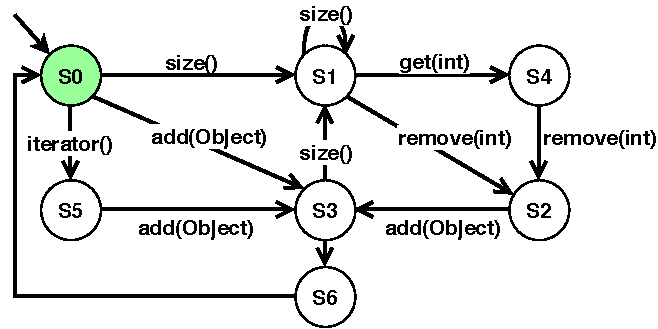
\includegraphics[width=0.55\textwidth]{papers/model_seeding/figures/list.pdf}
%    \vspace{-2mm}
    \caption{Transition system for method call sequences of the class \texttt{java.util.LinkedList} derived from Apache commons math source code and test cases.}
    \label{fig:list}
%    \vspace{-4mm}
\end{figure}

%Similarly to search-based testing, behavioral model-based testing seeks to select a relevant set of test cases.
\textit{Model-based testing} \cite{Utting2007} relies on abstract specifications (models) of the system under test to support the generation of relevant (abstract) test cases.  \textit{Transition systems} \cite{Baier2007} have been used as a fundamental formalism to reason about test case generation and support the definition of formal test selection criteria \cite{Tretmans2008}.
%
Each abstract test case corresponds to a sequence of method calls on one object: \ie a path in the transition system starting from the initial state and ending in the initial state, a commonly used convention to deal with finite behaviours \cite{Devroey2017b}.
Once selected from the model, abstract test cases are concretized (by mapping the transition system's paths to concrete sequences of method calls) into \emph{executable test cases} to be run on the system.
In this paper, we derive abstract test cases (called \emph{abstract object behavior} hereafter) and concretize them, producing pieces of code creating objects and invoking methods on such objects. Those pieces of code serve as seeds for search-based crash reproduction.

Figure \ref{fig:list} shows an example of a transition system representing the possible \emph{sequences} of method calls on \texttt{java.util.List} objects. Figure  \ref{fig:list} illustrates usages of methods in \texttt{java.util.List} objects, learned from the code and tests, in terms of a transition system, from which \textit{sequences} of methods calls can be derived.
%

The obtained transition system subsumes the behavior of the sequences used to learn it but also allows for new combinations of those sequences.  These behaviors are relevant in the context of seeding as the diversity of the objects induced is useful for the search process. Also, generating invalid behaviors from the new combinations is not a problem here as they are detectable during the search process.

%Derived sequences may correspond to the original sequences, but also combinations of those sequences. Hence the behavior described by the model is richer and subsumes the behavior of the sequences used to learn it. This property is very useful for seeding in search-based software testing as it allows better diversity of the objects, which helps during the search process.

%A transition system is composed of a set of states with an initial state ($s_0$ in Figure \ref{fig:list}) and transitions. Each transition may be labeled with an action, representing here a method call.


\subsubsection{Abstract object behavior selection}

The abstract object behaviors are selected from the transition system according to criteria defined by the tester. In the remainder of this paper, we use \emph{dissimilarity} as selection criteria~\cite{Cartaxo2011,Hemmati2013}.
Dissimilarity selection, which aims at maximizing the fault detection rate by increasing diversity among test cases, has been shown to be an interesting and scalable alternative to other classical selection criteria \cite{Hemmati2013, mondal2015}.
This diversity is measured using a dissimilarity distance (here, 1 - the Jaccard index \cite{Jaccard1901}) between the actions of two abstract object behaviors.

\subsubsection{Model Inference}

The model may be manually specified (and in this case will generally focus on specific aspects of the system) \cite{Utting2007}, or automatically learned from observations of the system \cite{Herbold2017, Leemans2018, Sprenkle2013, Sprenkle2011a, Tonella2014, Verwer2017}.
In the latter case, the model will be incomplete and only contain the \emph{observed behavior} of the system \cite{Tonella2012}. For instance, the sequence $<$\texttt{new}, \texttt{addAll} $>$ is valid for a \texttt{java.util.List} object but cannot be derived from the transition system in Figure \ref{fig:list} as the \texttt{addAll} method call has never been observed.
%
The observed behavior can be obtained via static analysis \cite{Fraser2011a} or dynamically \cite{Krka:2010:UDE:1810295.1810324}. Model inference may be used for visualization \cite{Leemans2018, Verwer2017}, system properties verification \cite{Lorenzoli2008a, Ghezzi2014}, or generation \cite{Herbold2017, Sprenkle2013, Sprenkle2011a, Prowell2004, Zhang2015a, Fraser2011a} and prioritization \cite{Devroey2017b, Dulz2003} of test cases.




% !TEX root =  ../STVR-model-seeding.tex

%%%%%%%%%%%%%%%%%%%%%%
 \section{Behavioral Model and Test Seeding for Crash Reproduction}
 \label{sec:model_seeding:approach}
 %%%%%%%%%%%%%%%%%%%%%%

The goal of behavioral model seeding (denoted model seeding hereafter) is to abstract the behavior of the software under test using models and use that abstraction during the search. At the unit test level (which is the considered test generation level in this study), each model is a transition system, like in Figure \ref{fig:list}, and represents possible usages of a class: \ie possible sequences of method calls observed for objects of that class.

\begin{figure*}[t]
    \centering
    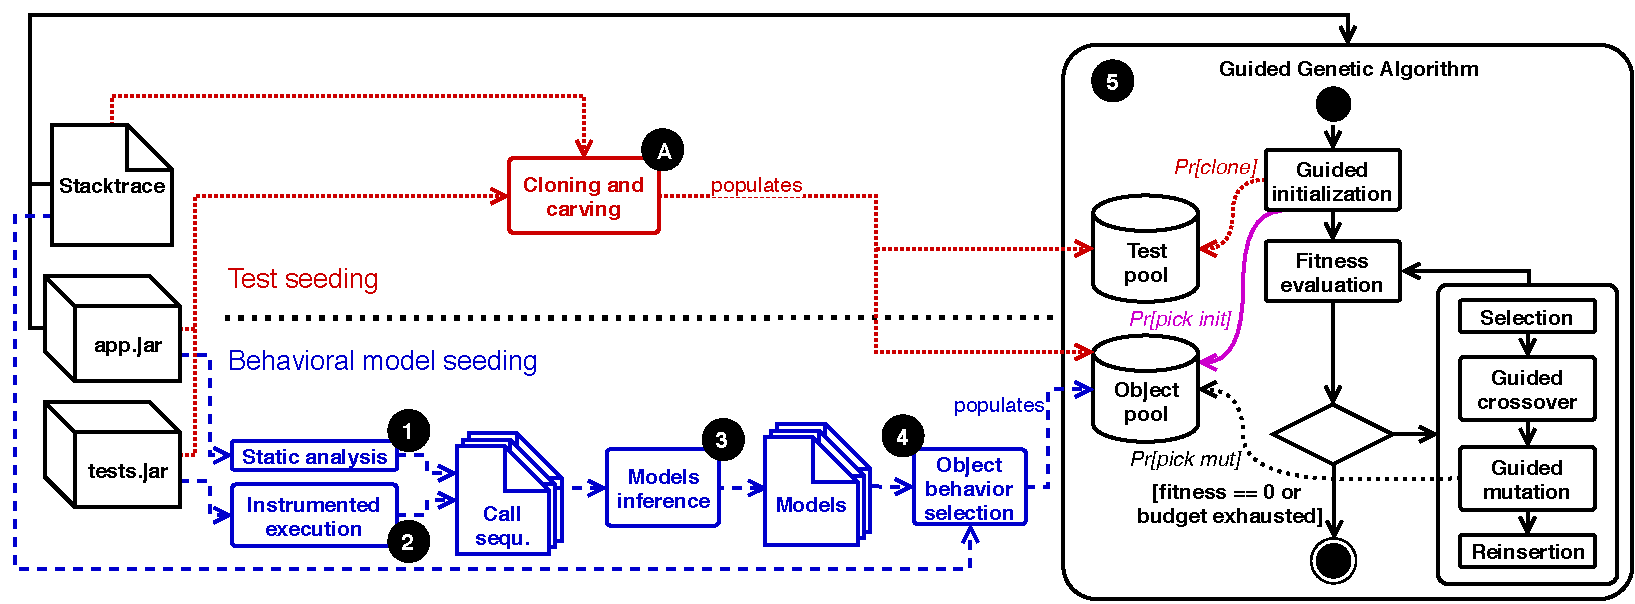
\includegraphics[width=\textwidth]{papers/model_seeding/figures/implementation/approach.pdf}
%    \vspace{-1mm}
    \caption{General overview of model seeding and test seeding for search-based crash reproduction}
    \label{fig:approach}
%    \vspace{-3mm}
\end{figure*}

The main steps of our model seeding approach, presented in Figure~\ref{fig:approach}, are:
 the \emph{inference} of the individual models \circled{3} (described in Section \ref{ssec:inference}) from the \emph{call sequences} collected through \emph{static analysis} \circled{1} performed on the application code (described in Section \ref{ssec:staticanalysis}), and \emph{dynamic analysis} \circled{2} of the test cases (described in Section \ref{ssec:dynamicanalysis});
 and for each model, the \emph{selection of abstract object behaviors} \circled{4}, that are concretized into Java objects  (described in Section \ref{ssec:abstract-selection}), stored in an \emph{object pool} from which the guided genetic algorithm \circled{5}  (described in Section \ref{ssec:gga}) can randomly pick objects to build test cases during the search process.

%--------------------------------
\subsection{Model inference}
\label{ssec:inference}
%--------------------------------

Call sequences are obtained by using static analysis on the bytecode of the application \circled{1} and by instrumenting and executing the existing test cases \circled{2}.

We use $n$-gram inference to build the transition systems used for model seeding. $N$-gram inference takes a set of sequences of actions as input to produce a transition system where the $n^{th}$ action depends on the $n-1$ previously executed actions.

%For  $2$-gram inference, the next action to execute only depends on the current state in the transition system. 

A large value of $n$ for the $n$-gram inference would result in wider transition systems with more states and less incoming transitions, representing a more constrained behavior and producing less diverse test cases. In contrast, a small  value of $n$ enables better diversity in the behavior allowed by the model (ending up in more diverse abstract object behaviors), requires less observations to reach stability of the model, simplifies the inference, and results in a more compact model~\cite{Sprenkle2013,Sprenkle2011a}.  For these reasons, we use $2$-gram inference to build our models. % used for model seeding.
%
%For instance, the transition system model in Figure~\ref{fig:list} has been partially generated from the following call sequences collected from the code and the test cases:
%
%{\ttfamily\footnotesize<size(), re\-move(), add(Ob\-ject), size(), size(), size(), get(), re\-move(), add(Ob\-ject)>};
%{\ttfamily\footnotesize<i\-te\-ra\-tor(),add(Ob\-ject)>}; \etc.
%
%Each transition in Figure~\ref{fig:list} corresponds to a method call in one of the sequences, and for each sequence, there exists a path in the model. % corresponding to that sequence.

%\andy{Should this choice for static and dynamic be better argumented? Why not use static for the test case as well?
%\pouria{I have tried to answer this question in subsection 4.1.2. We can move the answer here}
%}
%
For each class, the model \circled{3} is obtained using a  $2$-gram inference method using the call sequences of that class.

%
For instance, in the transition system of Figure \ref{fig:list}, the action \texttt{size()}, executed from state $s_3$ at step $k$ only depends on the fact that the action \texttt{add(Object)} has been executed at step $k-1$, independently of the fact that there is a step $k-2$ during which the action \texttt{iterator()} has been executed.

Calls to constructors are considered as method calls during model inference. However, constructors may not appear in any transition of the model if no constructor call was observed during the collection of the call sequences.  This is usually the case when the call sequences used to infer the model have been captured from objects that are parameters or attributes of a class. If an abstract object behavior does not start by a call to a constructor, a constructor is randomly chosen to initialize the object during the concretization.

% The model inference is a one time task. If any class changes in the future implementations, an extra analysis of the changed class will update the models.

For one version of the software under test, the model inference is a one time task. Models can then be directly reused for various crash reproductions.

\subsubsection{Static analysis of the application}
\label{ssec:staticanalysis}

The static analysis is performed on the bytecode of the application. We apply this analysis to all of the available classes in the software under test.  In each method of these classes, we build the control flow graph, and for each object of that method, we collect the sequences of method calls on that object.
For each object, each path in the control flow graph will correspond to one sequence of method calls. For instance, if the code contains an \texttt{if-then-else} statement, the \texttt{true} and \texttt{false} branches will produce two call sequences. In the case of a loop statement, the  \texttt{true} branch is considered only once. The static analysis is \emph{intraprocedural}, meaning that only the calls in the current method are considered. If an object is passed as a parameter of a call to a method that (internally) calls other methods on that object, those internal calls will not appear in the call sequences.
This analysis ensures collecting all of the existing relevant call sequences for any internal or external class, which is used in the project.

%The static analysis is performed on the bytecode of the application. To keep the process within a reasonable amount of time, we only apply this analysis to the classes involved in the stack trace.  In each method of these classes, we collect the sequences of method calls for all of the \andy{Should it be ``available'' or ``involved''?} \andy{Other question could be: how big is the gain in efficiency of the on-demand solution versus the ``do everything'' solution?} available classes. Since a stack trace represents a call hierarchy, this analysis ensures collecting relevant call sequences for at least the class at frame level $k$ in the methods of the class at frame level $k+1$. For instance, in the stack trace of Listing \ref{lst:model_seeding:stacktrace}, call sequences of \texttt{BaseObject} objects are collected (at least) in class \texttt{XWikiDocument}, which calls methods of  \texttt{BaseObject}.

\subsubsection{Dynamic analysis for the test cases}
\label{ssec:dynamicanalysis}

Since the existing manually developed test cases exemplify potential usage scenarios of the software under test, we apply dynamic analysis to collect all of the transpired sequences during the execution of these scenarios. Contrarily to static analysis, which would require an expensive effort and produce imprecise call sequences, dynamic analysis is \emph{interprocedural}. Meaning that the sequences include calls appearing in the test cases, but also internal calls triggered by the execution of the test case (\eg if the object is passed as a parameter to a method and methods are internally called on that object ). Hence, through dynamic analysis, we gain a more accurate insight into the class usages in these scenarios.

Dynamic analysis of the existing tests is done in a similar way to the carving approach of Rojas \etal~\cite{Rojas2016}: instrumentation adds log messages to indicate when a method is called, and the sequences of method calls are collected after execution. In similar fashion to static analysis, we collect call sequences of any observed object (even objects which are not defined in the software under test).
The representativeness of the collected sequences depends on the coverage of the existing tests.

%\andy{If this is still relevant, this MSc thesis shows that $\sim$80 of jUnit tests are actually integration tests. See my mattermost message Xavier...}
%\andy{I don't exactly know what you want... this article says that private methods are often tested indirectly. Is that what you are after?  (A Simple and Practical Approach to Unit Testing: The JML and JUnit Way, ECOOP 2002)}


%---------------------------------------------
\subsection{Abstract Object Behaviors Selection}
\label{ssec:abstract-selection}
%---------------------------------------------

Abstract object behaviors are selected from the transition systems and concretized to populate the object pool used during the search.
%
To limit the number of objects in the pool, we only select abstract object behaviors from two categories of models:  models of internal classes (\ie classes belonging to packages of the software under test) and models of dependency classes (\ie classes belonging to packages of external dependencies) that are involved in the stack trace.
Since we do not seek to validate the implementation of the application, the states are ignored during the selection process.

\subsubsection{Selection}
\label{ssec:selection}

There exist various criteria to select abstract object behaviors from transition systems~\cite{Utting2007}.
%
To successfully guide the search, we need to establish a good ratio between \emph{exploration} (the ability to visit new regions of the search space) and \emph{exploitation} (the ability to visit the neighborhood of previously visited regions) \cite{vcrepinvsek2013}.
The guided genetic operators which are introduced in the \evocrash approach \cite{soltani2017} guarantee the exploitation by focusing the search based on the methods in the stack trace. However, depending on the stack trace, focusing on particular methods may reduce the exploration. Poor exploration decreases the diversity of the generated tests and may trap the search process in local optima.

To improve the exploration ability in the search process, we use \emph{dissimilarity} as the criterion to select the abstract object behaviors. Compared to classical structural coverage criteria that seek to cover as many parts of the transition system as possible, dissimilarity tries to increase diversity among the test cases by maximizing a distance $d$ (\ie the Jaccard index \cite{Jaccard1901}):
$$
d = 1 - \frac{ \{call_{1i} \in b_{1}\} \cap \{call_{2j} \in b_{2}\}}{\{call_{1i} \in b_{1}\} \cup \{call_{2j} \in b_{2}\}}
$$
Where $b_{1} = <\mathit{call}_{11}, \mathit{call}_{12}, \ldots> $ and $ b_{2} = <\mathit{call}_{21}, \mathit{call}_{22}, \ldots>$ are two abstract object behaviors.

\subsubsection{Concretization}
\label{ssec:concretization}

Each abstract object behavior has to be concretized to an object and method calls before being added to the objects pool. In other words, for each abstract object behavior, if the constructor invocation is not the first action, one constructor is randomly called; and the methods are called on this object in the order specified by the abstract object behavior with randomly generated parameter values. Due to the randomness, each concretization may be different from the previous one. For each abstract object behavior, $n$ concretizations (default value is $n=1$  to balance scalability and diversity of the objects in the object pool) are done for each abstract object behavior and saved in the object pool.
%
For instance, Listing \ref{lst:concretized-test} shows the concretized abstract object behavior {\ttfamily\footnotesize <add(Object), add(Object)>} derived from the transition system model of Figure \ref{fig:list}. The type of the parameters (\texttt{EuclideanIntegerPoint}) is randomly selected during the concretization and created with required parameter values (an integer array here).


\begin{lstlisting}[
language=Java,
caption={Concretized abstract object behavior for \texttt{LinkedList} based on the transition system model of Figure \ref{fig:list}},
label=lst:concretized-test,
float=t]
int[] t = new int[7];
t[3] = -2147483647;
EuclideanIntegerPoint ep = new EuclideanIntegerPoint(t);
LinkedList<[...]> lst = new LinkedList<>();
lst.add(ep);
lst.add(ep);
\end{lstlisting}


%----------------------------------------------------------
\subsection{Guided Initialization and Guided Mutation}
\label{ssec:gga}
%----------------------------------------------------------

Classes are instantiated to create objects during two main steps of the guided genetic algorithm: guided initialization, where objects are needed to create the initial set of test cases; and guided mutation, where objects may be required as parameters when adding a method call. When no seeding is used, those objects are randomly created (as in the concretization step described in Section~\ref{ssec:concretization}) by calling the constructor and random methods.

Finally, to preserve exploration in model seeding, objects are picked from the object pool during guided initialization (resp. guided mutation) according to a user-defined probability $Pr[pick\ init]$ (resp. $Pr[pick\ mut]$), and randomly generated otherwise.
In our evaluation, we considered four different values for $Pr[pick\ init] \in \{0.2, 0.5, 0.8, 1.0\}$, to study the effect of model seeding on the initialization of the search process. Furthermore, we fixed the value of $Pr[pick\ mut] = 0.3$, corresponding to the default value of $Pr[pick\ mut]$ for test seeding for classical unit test generation in \evosuite.
%The value of the probability depends on the number and diversity of the concretized abstract object behaviors. For instance, a small model will deliver few different abstract object behaviors. In this case, lower probability values allow more randomly generated objects with calls to methods that do not appear in the model. In contrast, a large model, denoting complex behavior for the objects, may require higher probability values to avoid incorrect sequences of method invocations.



\begin{lstlisting}[
    numbers=left,
    caption={Stack trace excerpt for MATH-79b},
    label=lst:MATH-79b-trace,
    float=t]
    java.lang.NullPointerException
     at ...KMeansPlusPlusClusterer.assignPointsToClusters()
     at ...KMeansPlusPlusClusterer.cluster()
    \end{lstlisting}

\begin{lstlisting}[
language=Java,
escapechar=|,
caption={Test generated for frame 2 of MATH-79b (Listing \ref{lst:MATH-79b-trace})},
label=lst:generated-test,
float=t]
public void testCluster() throws Exception{
 int[] t = new int[7]; | \label{line:startobject} |
 t[3] = (-2147483647);
 EuclideanIntegerPoint ep = new EuclideanIntegerPoint(t);
 LinkedList<[...]> lst = new LinkedList<>();
 lst.add(ep);
 lst.add(ep); | \label{line:endobject} |
 KMeansPlusPlusClusterer<[...]> kmean = new KMeansPlusPlusClusterer<>(12);
 lst.offerFirst(ep); | \label{line:additional} |
 kmean.cluster(lst, 1, (-1357));} | \label{line:target} |
\end{lstlisting}



As an example of object picking in action, test case generation with model seeding generated the test case in Listing \ref{lst:generated-test} for the second frame of the stack trace from the crash MATH-79b from the Apache commons math project, reported in Listing \ref{lst:MATH-79b-trace}.
%
The target method is the last method called in the test (line \ref{line:target}) and throws a \texttt{NullPointerException}, reproducing the input stack trace. The first parameter of the method has to be a \texttt{Collection<T>} object. In this case, the guided genetic algorithm picked the list object from the object pool (from Listing \ref{lst:concretized-test}) and inserted it in the test case (lines \ref{line:startobject} to \ref{line:endobject}). The algorithm also modified that object (during guided mutation) by invoking an additional method on the object (line \ref{line:additional}).

%-----------------------------
 \subsection{Test Seeding}
%-----------------------------

As described in Section \ref{ssec:background:testseeding}, test seeding starts by executing the test cases (Figure \ref{fig:approach} box \circled{A}) for carving and cloning, and subsequently populating the test and object pools. Like for model seeding, only internal classes and external classes appearing in the stack trace are considered.

For crash reproduction, the test pool is used only during guided initialization to clone test cases that contain the target class, according to a user-defined $Pr[clone]$ probability. If the target method is not called in the cloned test case, the guided initialization also mutates the test case to add a call to the target method.
%
The object pool is used during the guided initialization and guided mutation to pick objects. 
As described by Rojas \etal~\cite{Rojas2016}, the properties of using the object pool during initialization ($Pr[pick\ init]$) and mutation ($Pr[pick\ mut]$) are indicated as a single property called \texttt{p\_object\_pool} in test seeding.


%------------------------------------------------------------------------
% \subsection{Comparison between behavioral model seeding and test seeding}
%------------------------------------------------------------------------

%Behavioral model seeding exploits both test cases and source code, thereby \emph{subsuming} test seeding regarding the observed behavior of the application that is reused during the search. Test seeding only uses dynamic analysis, which entails that it collects more accurate information from the potential usage scenarios of the software under test; it also means that this strategy collects more limited information for seeding. If these limited amounts of call sequences differ from the call sequences needed to reproduce the crash scenario, test seeding can misguide the crash reproduction search process.
%
%For instance, to initialize a \texttt{List} like in Listing~\ref{lst:generated-test}, test seeding can only seed the call sequences which are observed during the execution of the test cases, while model seeding can use any path in the transition system of Figure~\ref{fig:list}, which is inferred from all of the collected call sequences from static and dynamic analysis, for seeding. Using more call sequences for seeding helps behavioral model seeding to have accurate knowledge about the usage of the \texttt{List} class.
%However, by using cloning, test seeding benefits from (fixed) readily usable objects during initialization at the expense of diversity.
%\andy{mmm... what about something you also mentioned earlier... the fact that the models that come from testing are more ``precise'' and less ``open'' than those obtained statically?
%\pouria{model seeding uses the collected call sequences from both static and dynamic analysis while test seeding only uses the collected call sequences of dynamic analysis. Since more call sequences help us to have more accurate information about the class usages, we think that model seeding has more chance to cover the crash path. I tried to extend this section to explain this point more specifically. Also, I have added this discussion in the motivation section. In addition, I rephrased the section which discusses the ``precise" results of dynamic analysis (Section 4.1.2)}
%}

%Since test seeding only considers the fixed method calls sequences observed in the test cases to initialize the objects, model seeding \emph{subsumes} test seeding as it analyzes both test cases and source code for this purpose.
%In addition, even when only using the existing test cases, model seeding, which abstracts the behavior compared to test seeding,  can generate more objects with different behavior compared to test seeding.
%%
%For instance, to initialize a list like in Listing~\ref{lst:generated-test}, test seeding can only seed the call sequences which are observed during the execution of the test cases, while model seeding can use any path in the transition system of Figure~\ref{fig:list} for seeding.

% !TEX root =  ../STVR-model-seeding.tex

%%%%%%%%%%%%%%%%%%%%%%
\section{Implementation}\label{sec:model_seeding:implementation}
%%%%%%%%%%%%%%%%%%%%%%

%Based on the \evocrash approach and our re-engineering of the \evocrash tool, we developed \botsing, a framework for crash reproduction.
%We had two main goals for developing \botsing.
%Firstly, we wanted a more stable and well-tested toolset for crash reproduction. For Botsing, we have achieved 83\% branch coverage for the key \textit{botsing reproduction} module by unit testing. During the testing process, we found and fixed many bugs which affected the performance of the search process.
%Secondly, we aimed for an extendable framework for crash reproduction and other search-based testing problems. Similar to \evocrash, \botsing relies on \evosuite~\cite{Fraser2011} for the code instrumentation during test generation and execution. However, \botsing only uses \textit{evosuite-client} as a dependency, while \evocrash was an extension of \evosuite itself.
%Our open-source implementation is available at \url{https://github.com/STAMP-project/botsing}. The current version of \botsing includes both test seeding and model seeding as features.

%Based on the \evocrash approach, we developed \botsing, an extendable framework for crash reproduction.
% \botsing relies on \evosuite~\cite{Fraser2011} for the code instrumentation during test generation and execution %by using \textit{evosuite-client} as a dependency.
%Our open-source implementation is available at \url{https://github.com/STAMP-project/botsing}. The current version of \botsing includes both test seeding and model seeding as features.

Relying on the \evocrash experience (Chapter 2),  we developed \botsing, a framework for crash reproduction with extensibility in mind.
 \botsing also relies on \evosuite~\cite{Fraser2011} for the code instrumentation during test generation and execution by using \textit{evosuite-client} as a dependency.
Our open-source implementation is available at \url{https://github.com/STAMP-project/botsing}. The current version of \botsing includes both test seeding and model seeding as features.



%-----------------------------------
\subsection{Test Seeding}
%-----------------------------------

Test seeding relies on the implementation defined by Rojas \etal~\cite{Rojas2016} and available in \evosuite. This implementation requires the user to provide a list of test cases to consider for cloning and carving. In \botsing, we automated this process using the dynamic analysis of the test cases to automatically detect those accessing classes involved in a given stack trace. We also modified the standard guided initialization and guided mutation to preserve the call to the target method during cloning and carving.

%-----------------------------------
\subsection{Model Seeding}
%-----------------------------------

% Add this to the setup part
%During the static analysis, we collect the used objects in each of the test cases too. This information is used in the dynamic analysis to keep this process within a reasonable amount of time.
As mentioned in Section~\ref{sec:model_seeding:approach}, \botsing uses a combination of static and dynamic analysis to infer models. The static analysis (\circled{1} in Figure \ref{fig:approach}) uses the reflection mechanisms of \evosuite to inspect the compiled code of the classes involved in the stack traces, and collect call sequences. The dynamic analysis (\circled{2} in Figure \ref{fig:approach}) relies on the test seeding mechanism used for cloning that allows inspecting an internal representation of the test cases obtained after their execution and collect call sequences.
%
The resulting call sequences are then used to infer the transition system models of the classes using a 2-gram inference tool called YAMI~\cite{Devroey2017b} (\circled{3} in Figure \ref{fig:approach}).
From the infered models, we extract a set of dissimilar (based on the Jaccard distance \cite{Jaccard1901}) abstract object behaviors (\circled{4} in Figure \ref{fig:approach}). For abstract object behavior extraction, we use the VIBeS~\cite{Devroey2016} model-based testing tool.
%
Abstract object behaviors are then concretized into real objects. For this concretization, we rely on the EvoSuite API.

%A set of abstract object behaviors are selected from each of the models using a dissimilarity criterion (based on the Jaccard distance \cite{Jaccard1901}), taken from VIBeS~\cite{Devroey2016}, a model-based testing tool, working with transition systems.

%
% \todo{The following sentences are not clear. Explain that this is an implementation detail and that we could directly generate and concretize new abstract object behaviors each time.
% From Gilles: updated below.  $Pr[pick\ init]$ and $Pr[pick\ mut]$ need to be defined, though}.



% We rely on the \evosuite API to concretize abstract object behaviors into objects for the objects' pool. $Pr[pick\ init]$ and $Pr[pick\ mut]$ are user-defined probabilities to select objects during the guided genetic algorithm execution in \botsing.


%
%If the size of this set is too small, the generated abstract object behaviors do not cover all of the transitions of the transition system. Also, using a small set of test cases can misguide the search process. On the contrary, if the size of the set is too large, the test concretization can become a time taking process.
%In this study, the size of this set is equivalent to the size of the individual population to make sure that we have enough test case to seed into the first population even if $Pr[pick\ init]$ is set to 1.0.
%
%The concretization of the test cases into objects for the objects pool is done using the \evosuite API to create Java unit tests. The objects are then picked during the guided genetic algorithm execution in \botsing with user-defined probabilities $Pr[pick\ init]$ and $Pr[pick\ mut]$.

% !TEX root =  ../STVR-model-seeding.tex
 
%%%%%%%%%%%%%%%%%%%%%%
\section{Empirical Evaluation}\label{sec:model_seeding:setup}
%%%%%%%%%%%%%%%%%%%%%%

Our evaluation aims to assess the effectiveness of each of the mentioned seeding strategies (model and test seeding) on search-based crash reproduction.
For this purpose, first, we evaluate the impact of each seeding strategy on the number of reproduced crashes. Second, we examine if using each of these strategies leads to a faster crash reproduction. Third, we see if each seeding strategy can help the search process to start more often. Finally, we characterize the impacting factors of test and model seeding.

Since the focus of this study is using seeding to enhance the guidance of the search initialization, we examine different probabilities of using the seeded information during the guided initialization in the evaluation of each strategy. Hence, we repeat each execution of test seeding with the following values for $Pr[clone]$: 0.2, 0.5, 0.8, and 1.0. Likewise, we execute each execution of model seeding with the same values for $Pr[pick\ init]$ (which is the only property that we can use for modifying the probability of the object seeding in the initialization of model seeding).

% Behavioral model seeding exploits both test cases and source code, thereby \emph{subsuming} test seeding regarding the observed behavior of the application that is reused during the search. Test seeding only uses dynamic analysis, which entails that it collects more accurate information from the potential usage scenarios of the software under test but only relies on call sequences found in the existing tests. If these call sequences differ from the call sequences needed to reproduce the crash scenario, test seeding can misguide the crash reproduction search process.

%----------------------
\subsection{Research questions}
\label{sec:model_seeding:setup:rqs}
%----------------------

In order to assess the usage of test seeding applied to crash reproduction and our new model seeding approach during the guided initialization, we performed an empirical evaluation to answer the two research questions defined in introduction of this chapter.

\medskip \textbf{RQ1} \emph{What is the influence of test seeding used during initialization on search-based crash reproduction?}
%
To answer this research question, we compare \botsing executions with \emph{test seeding} enabled to executions where no additional seeding strategy is used (denoted \emph{no seeding} hereafter), from their effectiveness to reproduce crashes and start the search process, the factors influencing this effectiveness, and the impact of test seeding on the efficiency. We divide \textbf{RQ1}  into four sub-research questions:
%
\begin{compactitem}
    \item[\textbf{RQ1.1}] Does test seeding help to reproduce more crashes?
    \item[\textbf{RQ1.2}] Does test seeding impact the efficiency of the search process?
    \item[\textbf{RQ1.3}] Can test seeding help to initialize the search process? 
    \item[\textbf{RQ1.4}] Which factors in test seeding impact the search process?
\end{compactitem}

\medskip \textbf{RQ2}  \emph{What is the influence of behavioral model seeding used during initialization on search-based crash reproduction?}
%
To answer this question, we compare \botsing executions with \emph{model seeding} to executions with \emph{test seeding} and \emph{no seeding}. We also divide \textbf{RQ2}  into four sub-research questions:
%
\begin{compactitem}
    \item[\textbf{RQ2.1}] Does behavioral model seeding help to reproduce more crashes compared to no seeding?

    \item[\textbf{RQ2.2}] Does behavioral model seeding impact the efficiency of the search process compared to no seeding?
    \item[\textbf{RQ2.3}] Can behavioral model seeding help to initialize the search process compared to no seeding? 
    \item[\textbf{RQ2.4}] Which factors in behavioral model seeding impact the search process?
\end{compactitem}


%----------------------
\subsection{Setup}
\label{sec:setup:setup}
%----------------------

\subsubsection{Crash selection}
\label{sec:setup:setup:selection}
In Chapter 2, we introduced a new benchmark, called \jcrashpack, containing 200 real-world crashes from seven projects: 
\textit{JFreeChart}, a framework for creating interactive charts; 
\textit{Commons-lang}, a library providing additional utilities to the \texttt{java.lang} API;
\textit{Commons-math}, a library of mathematics and statistics components; 
\textit{Mockito}, a testing framework for object mocking; 
\textit{Joda-time}, a library for date and time manipulation; 
\textit{XWiki}, a popular enterprise wiki management system; 
and \textit{ElasticSearch}, a distributed RESTful search and analytics engine.
We use the same benchmark for the empirical evaluation of model-seeding and test-seeding on crash reproduction.


To use test and model seeding for reproducing the crashes of \jcrashpack, first, we needed to apply static and dynamic analysis on different versions of projects in this benchmark. We successfully managed to run static analysis on all of the classes of \jcrashpack.
On the contrary, we observed that dynamic analysis was not successful in the execution of existing test suites of ElasticSearch. The reason for this failure stemmed from the technical difficulty of running ElasticSearch tests by the EvoSuite test executor. 
Since both of the seeding strategies need dynamic analysis, we excluded ElasticSearch cases from \jcrashpack for this experiment. 
\jcrashpack contains 122 crashes after excluding ElasticSearch cases. Table~\ref{tab:projects} provides more details about our dataset.

We used the selected crashes for the evaluation of \emph{no seeding} and \emph{model seeding}. Since \emph{test seeding} needs existing test cases that are using the target class, we filtered out the crashes which contain only classes without any using tests. Hence, we used only 59 crashes for the evaluation of \emph{test seeding}. More information about average number of used test classes for test seeding is available in Table \ref{tab:seeding-info}.


% In the recent study about applying an empirical evaluation
% In the earliest \evocrash empirical study \cite{soltani2017}, Soltani \etal used a benchmark consisting of 50 crashes. They compared their search-based approach with the other crash reproduction approaches using this benchmark. They demonstrated that \evocrash could replicate 82\% of the crashes. Considering that this benchmark was not enough challenging, they introduced a new benchmark, which contains more complex and more realistic crashes \cite{Soltani2018b}. The new benchmark includes 33 stack traces from 5 open source projects. They demonstrated that \evocrash has a lower crash reproduction rate in the new benchmark. For example, \evocrash cannot replicate 12 crashes by setting any frame as the target frame.

% For the empirical evaluation of model-seeding and test-seeding, we extend the most recent benchmark by Soltani et al~\cite{Soltani2018b} to 122 crashes by collecting new stack traces from the same projects.
%  In this extended benchmark, 26 new crashes are mined from XWiki (an open-source enterprise wiki) issue tracker.\footnote{See \url{https://jira.xwiki.org/}.} We make sure that our benchmark covers all of the available stack traces from \textit{XWiki 7.0} to \textit{Xwiki 9.X} (\ie, the latest version available at the time that we were extending the benchmark). The other crashes are gathered from Defects4j. Our benchmark includes all of the crashes in Defects4j which manifest a crash. Table~\ref{tab:projects} provides more details about our extended benchmark.

%(\textbf{Cr.}) used for the evaluation, with, for each one: the average number of frames in the stack traces of the crashes ($\overline{\mathbf{frm}}$), the average cyclomatic complexity ($\overline{\mathbf{CCN}}$), the average number of lines of code ($\overline{\mathbf{LOC}}$), the average line coverage of the existing test cases ($\overline{\mathbf{LC}}$), and the average branch coverage of the existing test cases ($\overline{\mathbf{BC}}$).

\begin{table} [t]
    \centering
	\caption{Projects used for the evaluation with the number of crashes (\textbf{Cr.}), the average number of frames per stack trace ($\overline{\mathbf{frm}}$), the average cyclomatic complexity ($\overline{\mathbf{CCN}}$), the average number of statements ($\overline{\mathbf{NCSS}}$), the average line coverage of the existing test cases ($\overline{\mathbf{LC}}$), and the average branch coverage of the existing test cases ($\overline{\mathbf{BC}}$).}
    \footnotesize
	\begin{tabular}{l rrrrrr}
\textbf{Application} & \textbf{Cr.} & $\overline{\mathbf{frm}}$ & $\overline{\mathbf{CCN}}$ & $\overline{\mathbf{NCSS}}$& $\overline{\mathbf{LC}}$ & $\overline{\mathbf{BC}}$ \\ 
\hline 
JFreeChart            &   2 & 6.00 & 2.79 & 63.01k & 67\% & 59\% \\ 
Commons-lang    &   22 & 2.04 & 3.28 & 13.38k & 91\% & 87\% \\ 
Commons-math   &   27 & 3.92 & 2.43 & 29.98k & 90\% & 84\% \\ 
Mockito                 &   12 & 5.08 & 1.79 & 6.06k & 97\% & 93\% \\ 
Joda-Time            &   8 & 3.87 & 2.11 & 19.41k & 89\% & 82\% \\ 
XWiki                    &  51 & 27.45 & 1.92 & 181.68k & 73\% & 71\% \\ 
\end{tabular}
	\label{tab:projects}
\end{table}

\begin{table}[t]
    \center
    \caption{Information about test classes and models used, respectively, for test and model seeding in each project. $\overline{test}$ designate the average number of test classes used for test seeding. Also, $\overline{state}$, $\overline{trans}$, and $\overline{BFS}$ denote the average number of states, transitions, and BFS height of the used models, respectively. The standard deviations of each of these metrics ($\sigma$) are located beside them.}
    \label{tab:seeding-info}
    \footnotesize
    \begin{tabular}{ l | r r}
\hline 
\textbf{Project} & \textbf{$\overline{test}$} & \textbf{$\sigma$} \\ 
\hline 
chart  &  29.17  &  20.01\\ 
lang  &  1.45  &  2.03\\ 
math  &  1.24  &  1.37\\ 
mockito  &  0.73  &  2.15\\ 
time  &  9.24  &  9.55\\ 
xwiki  &  0.14  &  1.09\\ 
\end{tabular}
    \begin{tabular}{ l | r r r r r r}
\hline 
\textbf{Project} & \textbf{$\overline{state}$} & \textbf{$\sigma$} & \textbf{$\overline{trans}$} & \textbf{$\sigma$} & \textbf{$\overline{BFS}$} & \textbf{$\sigma$} \\ 
\hline 
chart  &  56.67  &  50.40  &  157.50  &  167.86  &  21.00  &  17.50\\ 
lang  &  39.69  &  51.49  &  117.96  &  158.07  &  5.58  &  7.32\\ 
math  &  14.00  &  12.46  &  34.22  &  40.59  &  5.20  &  4.11\\ 
mockito  &  12.18  &  10.93  &  21.45  &  22.70  &  5.32  &  3.90\\ 
time  &  63.35  &  40.85  &  230.80  &  167.99  &  16.10  &  11.79\\ 
xwiki  &  47.94  &  90.94  &  139.15  &  323.75  &  11.08  &  17.04\\ 
\end{tabular}
\end{table}

\subsubsection{Model inference}
Since the selected crashes for this evaluation are identified before the model inference process, we have applied the dynamic analysis only on the test cases which use the classes involved in the crashes. During the static analysis, we spot all relevant test cases which call the methods of the classes that have appeared in the stack traces of the crashes. Next, we apply dynamic analysis only on the detected relevant test cases.
This filtering process helps us to shorten the model inference execution time without losing accuracy in the generated models.

More information about the inferred models is available in Table \ref{tab:seeding-info}.



\subsubsection{Configuration parameters}

We used a budget of 62,328 fitness evaluations (corresponding on average to 15 minutes of executing \botsing with no seeding on our infrastructure which is introduced in Section \ref{sec:setup:setup:infrst}) to avoid side effects on execution time when executing \botsing on different frames in parallel.
We also fixed the population size to 100 individuals as suggested by the latest study on search-based crash reproduction~\cite{Soltani2018b}.
% \todo{From Gilles: maybe also add that having the same number of individuals is useful for comparison with \evocrash?} 
%\andy{Why? What are the reasons? What are the potential consequences?
%\pouria{We used the same configurations as our SSBSE paper. However, the best population for the search-based crash reproduction is still an open issue to study.}
%\pouria{I have cited our SSBSE paper.}
%}
All other configuration parameters are set at their default value~\cite{Rojas2016}, and we used the default weighted sum scalarization fitness function (Equation \ref{fitness_function}) from Soltani \etal \cite{Soltani2018b}.

For test seeding executions, as we described at the beginning of this section, we execute each execution with four values for $Pr[clone]$: 0.2 (which is the default value), 0.5, 0.8, and 1.0. Also, we used the default value of 0.3 for \texttt{p\_object\_pool}.

% \paragraph{Test seeding}

% During the guided initialization of the algorithm, test seeding can clone test cases according to a user-defined probability $Pr[clone]$. In addition to the default 0.2 value, we executed model seeding with values 0.5, 0.8, and 1.0 for $Pr[clone]$. In the current \evosuite implementation, both $Pr[pick\ init]$ and $Pr[pick\ mut]$ are indicated as a single property called \texttt{p\_object\_pool}.
% This property indicates the probability of using the object pool during test generation (either during initialization or mutation).
% We left the default value of 0.3 for \texttt{p\_object\_pool}, and we only changed the value of $Pr[clone]$ in different configurations. Assessing the influence of test seeding on mutation is part of our future work. 
% \paragraph{Model seeding}

We also use values  0.2, 0.5, 0.8, and 1.0 for $Pr[pick\ init]$ for model seeding executions. The value of $Pr[pick\ mut]$, which indicates the probability of using seeded information during the mutation, is fixed at 0.3. In addition to model seeding configurations, we fix the size of the selected abstract object behaviors to the size of the individual population in order to ensure that there are enough test cases to initiate the search.




% As discussed in Section \ref{sec:approach}, model seeding does not clone the test cases in the initial population. It only has the probability of using the collected objects in the object pool during the test generation. 
%  $Pr[pick\ init]$ indicates the probability of using object pool in the guided initialization, and $Pr[pick\ mut]$ means the probability of using object pool during the guided mutation.
% Since the focus of this study is using seeding to enhance the guidance of the search initialization, and $Pr[pick\ init]$ is the only property that we can use for modifying the probability of the object seeding in initialization, we use the following values for $Pr[pick\ init]$: 0.2, 0.5, 0.8, 1.0. The value of $Pr[pick\ mut]$  is fixed to 0.3.

%\andy{Should we make it explicit for the reader why the $Pr[pick\ init]$ is differently configured for test seeding versus model seeding?
%\pouria{I have added the reason.}
%}


For each frame (951 in total), we executed \botsing for \emph{no seeding} (\ie no additional seeding compared to the default parameters of \botsing) and each configuration of \emph{model seeding}. 
%\andy{Each configuration... has that been explained sufficiently?
%\pouria{I have moved this discussion to the end of this subsubsection. The configurations of model seeding and test seeding are explained in the previous paragraphs.}
%}
Since \emph{test seeding} needs existing test cases which are using the target class, we filtered out the frames that do not have any test for execution of this seeding strategy. Therefore, we executed each configuration of \emph{test seeding} on the subset of frames (171 in total). 


\subsubsection{Infrastructure}
\label{sec:setup:setup:infrst}
We used 2 clusters (with 20 CPU-cores, 384 GB memory, and 482 GB hard drive) for our evaluation. For each stack trace, we executed an instance of \botsing for each frame which points to a class of the application. We discarded other frames to avoid generating test cases for external dependencies. 
We ran \botsing on 951 frames from 122 stack traces for no-seeding and each model-seeding strategy configuration. Also, we ran \botsing with test-seeding on 171 frames from 59 crashes. To address the random nature of the evaluated search approaches, we repeated each execution 30 times.
We executed a total of 186,560 independent executions for this study. These executions took about 18 days overall.


%-------------------------------------------
\subsection{Data analysis procedure} 
\label{sec:setup:analyzing}
%-------------------------------------------

To check if the search process can reach a better state using seeding strategies, we analyze the status of the search process after executing each of the cases (each run in one frame of a stack trace). We define 5 states: % for the status of the search process: 
% 
\begin{compactenum}[(i)]
\item \textbf{not started}, the initial population could not be initialized, and the search did not start;
\item \textbf{line not reached}, the target line could not be reached;
\item \textbf{line reached}, the target line has been reached, but the target exception could not be thrown;
\item \textbf{ex. thrown}, the target line has been reached, and an exception has been thrown but produced a different stack trace; and 
\item \textbf{reproduced} the stack trace could be reproduced.
\end{compactenum}
%
Since we repeat each execution 30 times, we use the majority of outcomes for a frame reproduction result. For instance, if \botsing reproduces a frame in the majority of the 30 runs, we count that frame as a \textit{reproduced}. 


To measure the impact of each strategy in the crash reproduction ratio (\textbf{RQ1.1} and \textbf{RQ2.1}), we use the Odds Ratio (OR) because of the binary distribution of the related data:  a search process either reproduces a crash (the generated test replicates the stack trace from the highest frame which is reproduced by at least one of the other searches) or not. Also, we apply Fisher's exact test, with $\alpha = 0.05$ for the Type I error, to evaluate the significance of results.

Moreover, to answer \textbf{RQ1.2} and \textbf{RQ2.2}, which investigate the efficiency of the different strategies, we compare the number of fitness function evaluations needed by the search to reach crash reproduction.
This metric indicates if seeding strategies lead to better initial populations that need fewer iterations to achieve the crash reproducing test. Since efficiency is only relevant for the reproduced cases, we only applied this comparison on the crashes which are reproduced at least once by no seeding or the seeding strategy (test seeding for \textbf{RQ1.2} and model seeding for \textbf{RQ2.2}).
 We use the Vargha-Delaney statistic \cite{vargha} to appraise the effect size between strategies. In this statistic, a value lower than 0.5 for a pair of factors $(A,B)$ gives that $A$ reduces the number of needed fitness function evaluations, and a value higher than 0.5 shows the opposite. Also, we use the Vargha-Delaney magnitude measure to partition the results into three categories having large, medium, and small impact. In addition, to examine the significance of the calculated effect sizes, we use the non-parametric Wilcoxon Rank Sum test, with  $\alpha = 0.05$  for Type I error. Moreover, we do note that since the reproduction ratio of each strategy is not 30/30 for each crash, executions that could not reproduce the frame simply reached the maximum allowed budget (62,328).


To measure the impact of each strategy in initializing the first population (\textbf{RQ1.3} and \textbf{RQ2.3}), we use the same procedure as \textbf{RQ1.1} and \textbf{RQ2.1} because the distribution of related data in this aspect is binary too (\ie whether the search process can start the search or not).

For all of the statistical tests in this study, we only use a level of significance $\alpha = 0.05$.

Since the model inference (in model seeding) and test carving (in test seeding) techniques can be applied as one time processes before running any search-based crash reproduction, we do not include them in the efficiency evaluation.

To answer \textbf{RQ1.4} and \textbf{RQ2.4}, we performed a manual analysis on the logs and crash reproducing test case (if any). We focused our manual analysis on the crash reproduction executions for which the search in one seeding configuration has a significant  impact (according to the results of the previous sub-research questions) on 
\begin{inparaenum}[(i)]
\item \textit{initializing the initial population},
\item \textit{crash reproduction},
\item or \textit{search process efficiency}
\end{inparaenum}
 compared to no-seeding.
Based on our manual analysis, we used a card sorting strategy by assigning keywords to each frame result and grouping those keywords to identify influencing factors.
% !TEX root =  ../STVR-model-seeding.tex

%%%%%%%%%%%%%%%%%%%%%%
\section{Evaluation Results}
\label{sec:model_seeding:eval-results}
%%%%%%%%%%%%%%%%%%%%%%



We present the results of the evaluation and answer the two research questions by comparing each seeding strategy with no-seeding.
%Figure \ref{fig:eval:results} presents the general results of our evaluation per crash. In Figure \ref{fig:eval:results-crashes}, The 122 crashes (100\%) are classified for each seeding configuration of model-seeding and no-seeding according to the outcome observed in the majority of the 30 executions. The model-seeding configurations refer to the different values used for $Pr[pick\ init]  \in \{0.2, 0.5, 0.8, 1.0\} $.

%(in Figure \ref{fig:eval:results-crashes}).
%The 122 crashes (100\%) are classified for each seeding configuration according to the outcome observed in the majority of the 30 executions.
%The configurations refer to the configuration used for seeding: no seeding (no s.), test seeding with $Pr[clone] \in \{0.2, 1.0\}$ (\textit{test s.}), and behavioral model seeding with $Pr[pick\ init]  \in \{0.2, 0.5, 0.8, 1.0\} $ (\textit{model s.}).


%\begin{table} [t]
%    \centering
%	\caption{Experiment results for no seeding, test seeding, and model seeding.}
%	\label{tab:results}
%	\begin{smaller}
%	
%%%%%%%%%%%%%%%%%%%%%%%%%%%%%%%%%%%%%%%%%%
\section{Results}
\label{sec:cub:results}
%%%%%%%%%%%%%%%%%%%%%%%%%%%%%%%%%%%%%%%%%%

\begin{figure}[t]
    \centering
    \subfloat[Test cases commonality scores.]{
        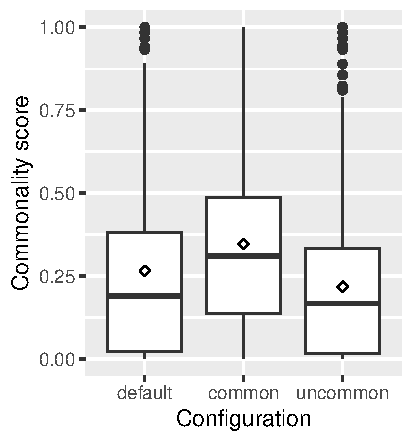
\includegraphics[height=50mm]{papers/cub/images/score.pdf}
        \label{subfig:score}
    }
    \subfloat[Effect sizes $\widehat{A}_{12}$ .]{
        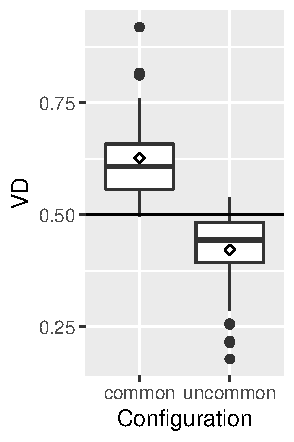
\includegraphics[height=50mm]{papers/cub/images/score-vd.pdf}
        \label{subfig:scorevd}
    }\\
    \subfloat[Effect sizes $\widehat{A}_{12}$ magnitudes.% (\textit{Significant differences $<0.05$}.
    ]{
        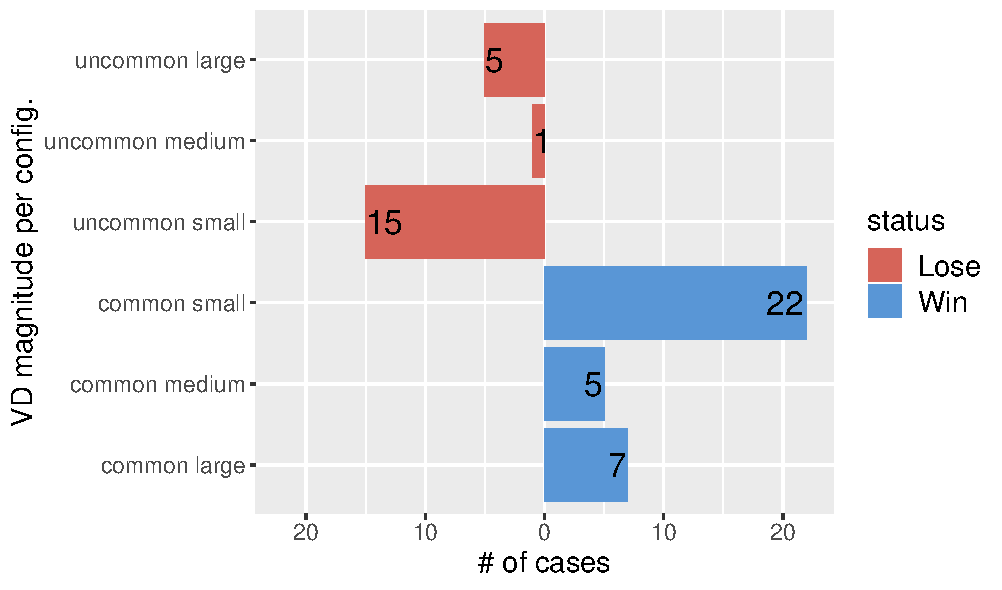
\includegraphics[height=50mm]{papers/cub/images/score-sig.pdf}
        \label{subfig:scoresig}
    } 
    
    \caption{Test cases commonality values and comparison to \df. Diamonds indicate mean values and horizontal bars (\textbf{--}) indicate median values.}
    \label{fig:rq1}
\end{figure}

\subsection{Commonality Score (RQ.1)}

In this section we answer the question: \emph{How does the \emph{commonality score} of the generated tests compare when using the \textit{common}, \textit{uncommon}, and \textit{default} secondary objectives?}

Figure \ref{fig:rq1} illustrates the impact of using \com and \ucom, as the secondary objective, on the commonality score of the generated test cases. Figure \ref{subfig:score} shows that the average and median of the commonality score is improved by 8\% and 12\%, respectively, compared to \df when using \com as secondary objective.
In parallel, using \ucom as secondary objective reduces the commonality score by, on average, 5\% (2.5\% for median) compared to \df. Moreover, Figure \ref{subfig:scoresig} presents the number of cases (\ie classes used as the target class for unit testing), in which the application of \com and \ucom significantly (\textit{p-value} $<0.05$) changes the commonality score with effect size magnitude of large, medium, or small. As we can see in this figure, utilizing \com always leads to a significant improvement in the commonality score (blue bars), and in contrast, using \ucom always reduces this score (red bars). In total, \com significantly improves the commonality score in 34 cases (32.6\% of classes), and \ucom significantly reduces this score in 21 classes (20.1\% of cases). Figure \ref{subfig:scorevd} depicts the effect sizes of differences observed in these cases. Consistent with the previous figures, the average effect size ($\widehat{A}_{12}$) achieved by \com is higher than 0.5 (\ie commonality score has been improved). However, this value is lower than 0.5 for \ucom.

\paragraph{Summary} Using \com as secondary objective in the \evosuite search-based test case generation process leads to test cases that exhibit an improved commonality score. In parallel, the application of \ucom leads to the reduction of the commonality score.

%-----------------------------------------
\subsection{Structural Coverage (RQ.2)}
%-----------------------------------------

In this section we provide an answer to the following research question: \emph{How does the \emph{line} and \emph{branch coverage} of the generated tests  compare when using the \textit{common}, \textit{uncommon}, and \textit{default} secondary objectives?}

Figure~\ref{fig:rq2} shows the line and branch coverage achieved by using \com and \ucom as secondary objectives compared to \df. Figure~\ref{subfig:coverage} indicates that the average coverage is the same for all of the assessed configurations.

Looking at the comparison of the structural coverage values achieved by each secondary objective in each class, we can see that the line and branch coverage is significantly impacted by \com and \ucom in some cases. Figure~\ref{subfig:coveragesig} presents the number of cases that these secondary objectives significantly (\textit{p-value} $<0.05$) reduce ($\widehat{A}_{12} < 0.5$) or increase ($\widehat{A}_{12} > 0.5$) the line and branch coverage with effect size magnitude small, medium, or large. According to this figure, in general, utilizing \com leads to a significant improvement for line and branch coverage in three and four classes, respectively. Nevertheless, this secondary objective reduced the line and branch coverage in eight and nine classes, respectively. 

Also, we can see a similar result for \ucom:
significant improvements in three and five classes and significant reductions in seven and nine cases for line and branch coverage. Since the number of cases in which \com and \ucom lead to a significantly lower structural coverage is higher than the the number of cases in which we see a significant improvement in coverage, the average effect size of differences (Figure~\ref{subfig:coveragevd}) is slightly less than  $0.5$ for both line (0.47 for both secondary objectives) and branch coverage (0.46 for both).

\paragraph{Summary} On average, using \com or \ucom does not impact the line and branch coverage. However, these two secondary objectives can significantly impact the structural coverage in specific cases.

\begin{figure}[t]
    \centering
    \subfloat[Test suites coverage and mutation score.]{
        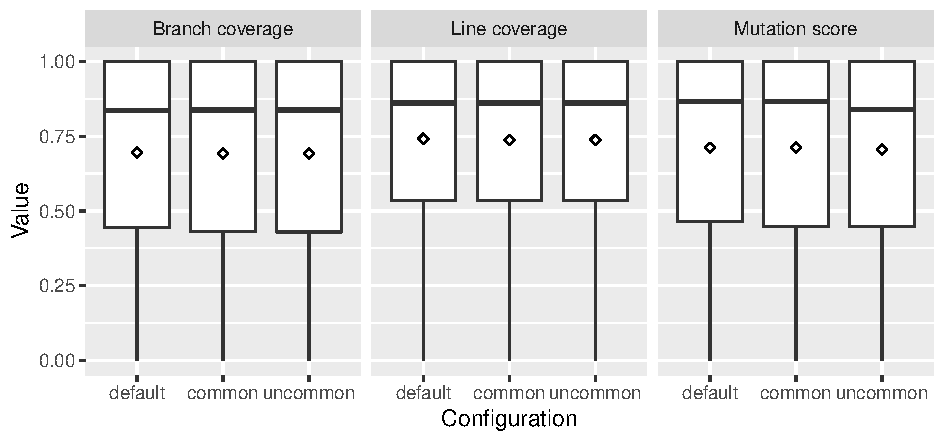
\includegraphics[height=30mm]{papers/cub/images/coverage.pdf}
        \label{subfig:coverage}
    }\hfill
    \subfloat[Effect sizes $\widehat{A}_{12}$.]{
        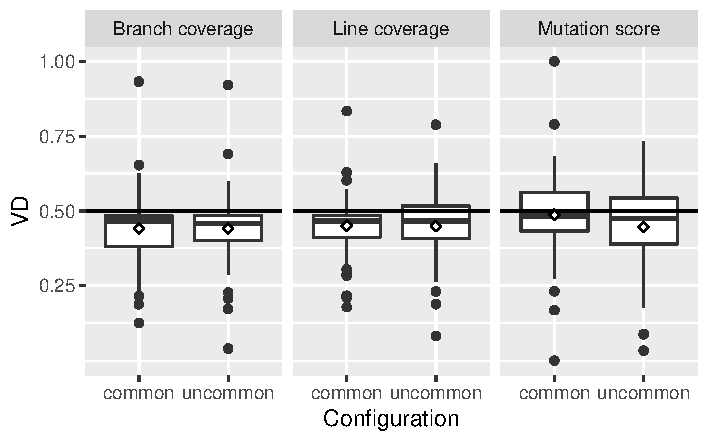
\includegraphics[height=30mm]{papers/cub/images/coverage-vd.pdf}
        \label{subfig:coveragevd}
    }\\ 
    \subfloat[Effect sizes $\widehat{A}_{12}$ magnitudes.]{
        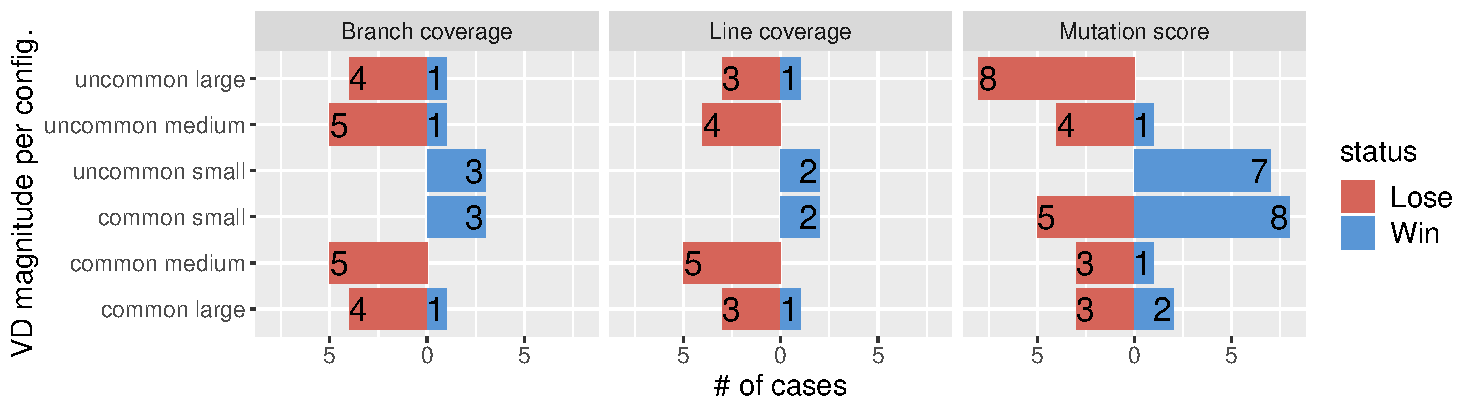
\includegraphics[height=30mm]{papers/cub/images/coverage-sig.pdf}
        \label{subfig:coveragesig}
    }
   
    \caption{Test suites coverage and mutation score, and comparison to \textit{default}. Diamonds indicate mean values and horizontal bars (\textbf{--}) indicate median values.}
    \label{fig:rq2}
\end{figure}

%-----------------------------------------
\subsection{Mutation Analysis (RQ.3)}
%-----------------------------------------

In the final research question we reflect on \emph{How does the \emph{mutation score} of the generated tests  compare when using the \textit{common}, \textit{uncommon}, and \textit{default} secondary objectives? }

Figure \ref{subfig:coverage} depicts the mutation score achieved by using \com and \ucom compared to \df. Like line and branch coverage, the average mutation scores achieved by these secondary objectives is similar to the one achieved by \df. 
However, Figure \ref{subfig:coveragesig} shows that \com and \ucom can significantly (\textit{p-value} $<0.05$) impact the mutation score achieved by unit test generation. The \com secondary objective significantly increases the number of mutants killed for 11 classes but, at the same time, also decreases the mutation score in another 11 cases. Moreover, \ucom significantly changes the mutation score in 20 cases (8 wins against 12 losses). 
Figure \ref{subfig:coveragevd} shows the effect size of differences in these cases for both \com and \ucom secondary objectives. According to this Figure, the average $\widehat{A}_{12}$ estimations are 0.49 and 0.47. Since these values are lower than 0.5, on average, the difference achieved by these two secondary objectives is negative. However, the outliers in this figure show us that the effect sizes of \com above 0.75 in some specific cases. Hence, the graphs in Figure~\ref{subfig:coveragesig} indicate that using \com and \ucom can improve the mutation score in specific cases.

\paragraph{Summary} On average, using \com or \ucom does not have any effect on the mutation score achieved by the generated test suites. However, these two secondary objectives can significantly change the killed mutants in some cases.
%	\end{smaller}
%\end{table}

%Figure \ref{fig:ffevals} presents the distribution of the number of fitness evaluations for the frames that could be reproduced by each seeding configuration in the 10 rounds of execution. The number of fitness evaluations varies between 0 (\ie the crash is reproduced by one of the test cases of the initial population) and 62,328 (\ie the maximum budget allocated for the search). For each box, we also provide the mean (represented as a white diamond) and number of observations (\ie the number of executions with a reproduction) at the top.

\begin{figure*}[btp]
	\centering
	\subfloat[test-seeding vs. no-seeding (for all projects together)]{
		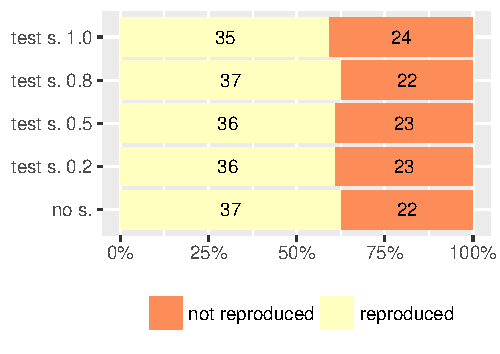
\includegraphics[height=40mm]{papers/model_seeding/figures/evaluation/rq12-crashes-all.pdf}
		\label{fig:eval:results-rq12}
	}\hfill  
	\subfloat[model-seeding vs. no-seeding (for all projects together)]{
		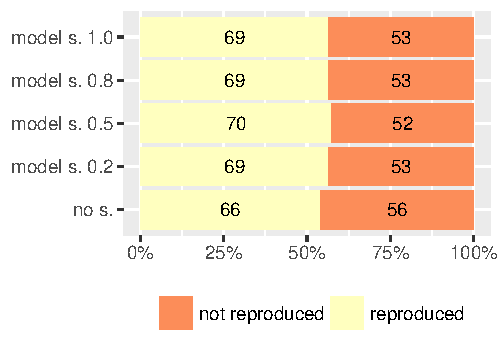
\includegraphics[height=40mm]{papers/model_seeding/figures/evaluation/rq22-crashes-all.pdf}
		\label{fig:eval:results-rq22}
	}

\subfloat[test-seeding vs. no-seeding (per project)]{
	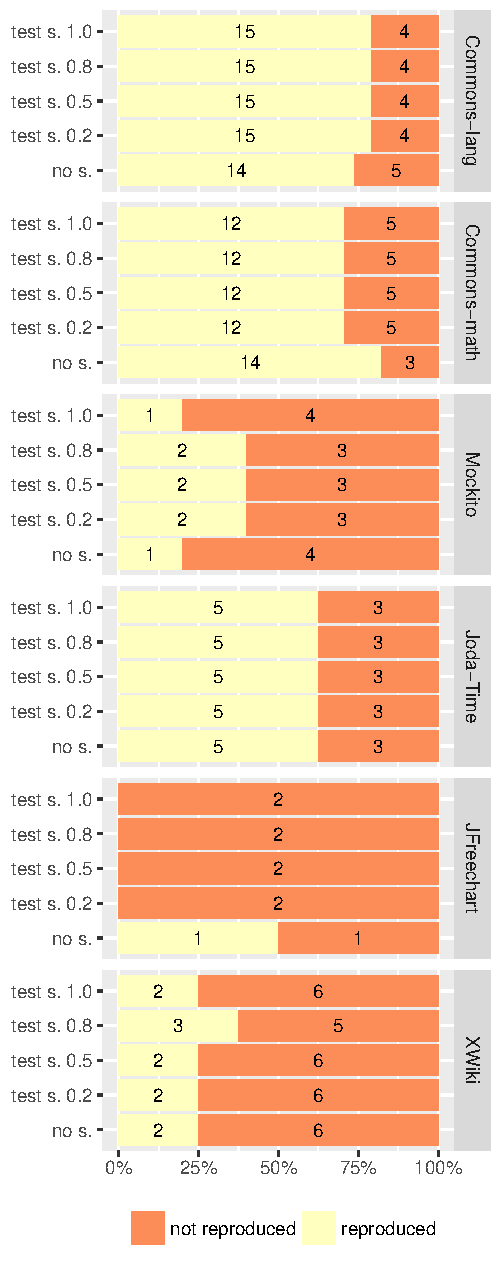
\includegraphics[height=130mm]{papers/model_seeding/figures/evaluation/rq12-crashes-apps.pdf}
	% \caption{test-seeding vs. no-seeding (per project)}
	\label{fig:eval:results-rq12-apps}
}\hfill
\subfloat[model-seeding vs. no-seeding (per project)]{
	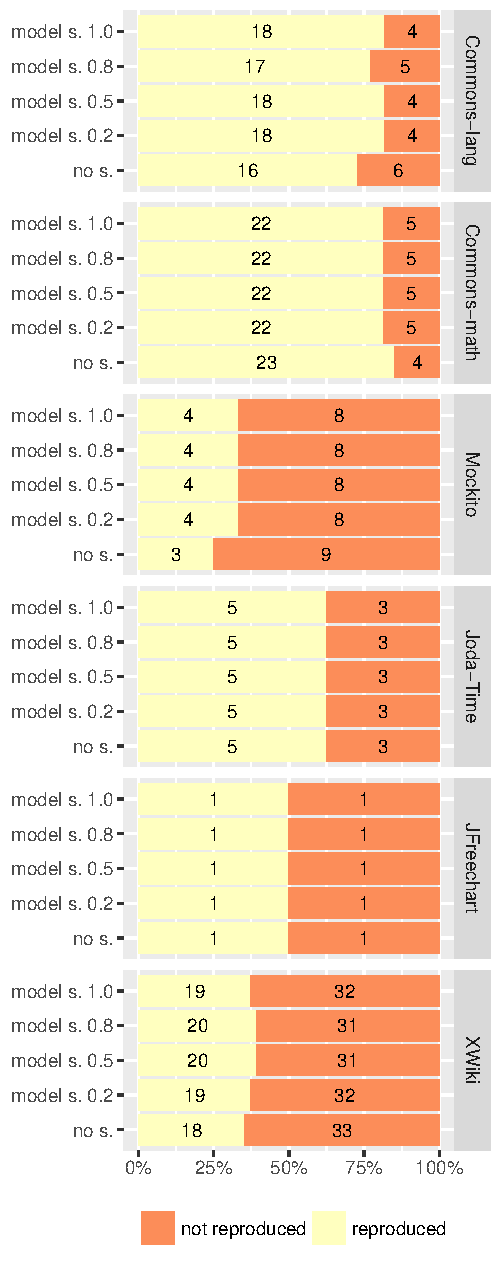
\includegraphics[height=130mm]{papers/model_seeding/figures/evaluation/rq22-crashes-apps.pdf}
	% \caption{test-seeding vs. no-seeding (per project)}
	\label{fig:eval:results-rq22-apps}
}
	\caption{Outcomes observed in the majority of the executions for each crash in total and for each application.}
%	\label{fig:eval:resultsdetails}
	\label{fig:eval:results}
\end{figure*}


%--------------------------------------------------------------------------------
\subsection{Test Seeding (RQ1)}
%--------------------------------------------------------------------------------

%\item[\textbf{RQ1.1}] Can test seeding help to initialize the search process?
%\item[\textbf{RQ1.2}] Does test seeding help to replicate more crashes?
%\item[\textbf{RQ1.3}] Does test seeding impact the efficiency of the search process?
%\item[\textbf{RQ1.4}] Which factors in test seeding help the search process compared to no seeding?



\begin{table}[t]
    \center
    \caption{Odds ratios of model/test seeding configurations vs. no seeding in crash reproduction ratio. This table only shows the crashes, which reveal statistically significant differences (p-value $< 0.05$). An Odds ratio value higher than 1.0 gives that the seeding strategy is better than no seeding, and a value lower than 1.0 shows the opposite.}
	\label{tab:oddratios}
	\footnotesize
	\subfloat{\begin{tabular}{ l | l | r}
\hline 
\textbf{Conf.} & \textbf{Crash} & \textbf{Odds Ratio (p-value)} \\ 
\hline 
test s. 0.5 & LANG-6b & Inf (2.37e-02)\\ 
 & MATH-1b & 0.00 (1.69e-17)\\ 
 & MATH-61b & 0.00 (1.69e-17)\\ 
 & CHART-4b & 0.00 (1.69e-17)\\ 
 & TIME-20b & 0.00 (1.94e-03)\\ 
 & TIME-10b & 207.79 (2.36e-12)\\ 
 & TIME-5b & 3.52 (3.52e-02)\\ 
\hline 
test s. 0.8 & LANG-6b & Inf (1.94e-03)\\ 
 & MATH-1b & 0.00 (1.69e-17)\\ 
 & MATH-61b & 0.00 (1.69e-17)\\ 
 & CHART-4b & 0.00 (1.69e-17)\\ 
 & TIME-20b & 0.00 (4.64e-05)\\ 
 & TIME-10b & Inf (9.23e-14)\\ 
 & TIME-7b & 0.00 (6.19e-07)\\ 
\hline 
test s. 1.0 & LANG-51b & 0.21 (8.21e-03)\\ 
 & LANG-6b & Inf (4.64e-05)\\ 
 & MATH-1b & 0.00 (1.69e-17)\\ 
 & MATH-61b & 0.00 (1.69e-17)\\ 
 & CHART-4b & 0.00 (1.69e-17)\\ 
 & TIME-20b & 0.00 (5.83e-06)\\ 
 & TIME-10b & 69.79 (2.82e-10)\\ 
\hline 
test s. 0.2 & MATH-1b & 0.00 (1.69e-17)\\ 
 & MATH-61b & 0.00 (1.69e-17)\\ 
 & CHART-4b & 0.00 (1.69e-17)\\ 
 & TIME-20b & 0.00 (3.19e-04)\\ 
 & TIME-10b & Inf (9.23e-14)\\ 
 & TIME-7b & 0.00 (1.05e-02)\\ 
\hline 
\end{tabular}}
    \subfloat{\begin{tabular}{ l | l | r}
\hline 
\textbf{Conf.} & \textbf{Crash} & \textbf{Odds Ratio (p-value)} \\ 
\hline 
model s. 0.2 & LANG-9b & Inf (1.94e-03)\\ 
 & LANG-51b & 0.17 (3.33e-03)\\ 
 & MOCKITO-10b & Inf (1.43e-08)\\ 
 & XWIKI-13141 & 13.95 (5.58e-03)\\ 
\hline 
model s. 0.5 & LANG-9b & Inf (2.37e-02)\\ 
 & MOCKITO-10b & Inf (1.87e-07)\\ 
 & XWIKI-13141 & Inf (7.97e-04)\\ 
 & XWIKI-14152 & 6.66 (7.41e-03)\\ 
\hline 
model s. 0.8 & LANG-9b & Inf (1.94e-03)\\ 
 & LANG-51b & 0.29 (3.70e-02)\\ 
 & MOCKITO-10b & Inf (8.27e-10)\\ 
 & XWIKI-13141 & Inf (7.97e-04)\\ 
 & XWIKI-14152 & 11.24 (2.51e-04)\\ 
\hline 
model s. 1.0 & LANG-9b & Inf (1.94e-03)\\ 
 & MOCKITO-10b & Inf (5.34e-08)\\ 
 & XWIKI-13141 & 13.95 (5.58e-03)\\ 
 & XWIKI-14152 & 32.80 (5.62e-08)\\ 
\hline 
\end{tabular}}
\end{table}



\subsubsection{Crash reproduction effectiveness (\textbf{RQ1.1})}

Figure~\ref{fig:eval:results} demonstrates the comparison of each seeding strategy (left-side of the figure is for test seeding and right-side is for model seeding) with the baseline (no seeding). Figures~\ref{fig:eval:results-rq12} and \ref{fig:eval:results-rq22} show the overall comparison, while Figures~\ref{fig:eval:results-rq12-apps} and~\ref{fig:eval:results-rq22-apps} illustrate the per project comparison. In each of these figures, the yellow bar shows the number of reproduced crashes in the majority of the 30 executions, and the orange bar shows the non-reproduced crashes.

According to Figure \ref{fig:eval:results-rq12}, \textit{test s. 0.8} reproduced the same number of crashes. However, the other configurations of test-seeding reproduced fewer crashes in the majority of times. Moreover, according to Figure \ref{fig:eval:results-rq12-apps}, test seeding reproduces one more crash compared to no seeding. Also, some configurations of test seeding can reproduce one extra crash in  XWiki and commons-lang projects. On the contrary, all of the configurations of test seeding missed one and two crashes in JFreeChart and commons-math, respectively. Finally, we cannot see any difference between test seeding and no seeding in the Joda-Time project.
 
 
 %Each of the observed differences in this figure is manually analyzed.
 %The observed factors in the manual analysis will be discussed in Section \ref{sec:eval:rq14}.

Table \ref{tab:crash-repr-table} demonstrates the impact of test-seeding on the crash reproduction ratio compared to no-seeding. It indicates that \textit{test s. 0.2 \& 0.5} have a better crash reproduction ratio for one of the crashes, while they perform significantly worse in 4 other crashes compared to no-seeding. The situation is almost the same for the other configurations of test seeding: \textit{test s. 0.8 \& 1.0} are significantly better in 2 crashes compared to no-seeding. However, they are significantly worse than no-seeding in 5 other crashes. The other interesting point in this table is the standard deviation crash reproduction ratio. This value is slightly higher for all of the test seeding configurations compared to no seeding. The values of odds ratios and and p-values for crashes with significant difference is available in Table \ref{tab:oddratios}.
%The cases which make the difference in this table are included in the manual analysis for Section \ref{sec:eval:rq14}.
%Table \ref{tab:reproduction-ranking} ranks the different configurations regarding their crash reproduction capability (\textbf{RQ1.2}). Only \textit{test s. 0.2} ranks better than no seeding, but not significantly. All other configurations are not significantly worse. Only test seeding with \textit{test s. 0.2} performs significantly better than \textit{test s. 0.5} and \textit{test s. 1.0}.

The underlying reasons for the observed results in this section are analyzed in \textbf{RQ1.4}.



\begin{table} [t]
	\center
	\caption{Evaluation results for comparing seeding strategies (test and model seeding) and no-seeding in crash reproduction. $\overline{\text{ratio}}$ and $\sigma$  designate average crash reproduction ratio and standard deviation, respectively. The numbers in the comparison only count the statistically significant cases.}
	\label{tab:crash-repr-table}
	\begin{footnotesize}
	\subfloat{\begin{tabular}{ l r r | r r r }
  \hline 
  \textbf{Conf.} & \multicolumn{2}{c|}{Reproduction} & \multicolumn{2}{c}{Comparison to no s.} \\ 
    & $\overline{\text{ratio}}$ & $\sigma$ & better & worse \\ 
  \hline 
  test s. 1.0 & 23.7 & 11.01 & 2 & 5 \\ 
  test s. 0.8 & 23.4 & 10.74 & 2 & 5 \\ 
  test s. 0.5 & 23.8 & 10.76 & 1 & 4 \\ 
  test s. 0.2 & 23.5 & 10.93 & 1 & 4 \\ 
  no s. & 25.4 & 9.65 & - & - \\ 
  \hline 
  \end{tabular}}
	\subfloat{\begin{tabular}{ l r r | r r r }
\hline 
\textbf{Conf.} & \multicolumn{2}{c|}{Reproduction} & \multicolumn{2}{c}{Comparison to no s.} \\ 
  & $\overline{\text{ratio}}$ & $\sigma$ & better & worse \\ 
\hline 
model s. 1.0 & 22.0 & 11.58 & 4 & 0 \\ 
model s. 0.8 & 21.9 & 11.92 & 4 & 1 \\ 
model s. 0.5 & 21.8 & 11.86 & 4 & 0 \\ 
model s. 0.2 & 21.6 & 12.00 & 3 & 1 \\ 
no s. & 21.3 & 12.32 & - & - \\ 
\hline 
\end{tabular}}
	
    \end{footnotesize}
\end{table}

\subsubsection{Crash reproduction efficiency (\textbf{RQ1.2})}

Table \ref{tab:fitness-evaluation-table} demonstrates the comparison of test-seeding and no-seeding in the number of needed fitness function evaluations for crash reproduction. The average number of fitness function evaluations increases when using test-seeding. It means that test-seeding is slower than no-seeding on average. \textit{test s. 0.8} has the highest average fitness function evaluations. 

Moreover, the standard deviations of both no seeding and test seeding are high values (more than 20k evaluations). This notable variation is explainable due to the nature of search-based approaches. In some executions, the initialized population is closer to the objectives, and the search process can achieve reproduction faster. Similar variations are reported in the \jcrashpack empirical evaluation as well (Chapter 2). According to the reported standard deviations, we can see that this value increases for all of the configurations of test seeding compared to no seeding.

Also, the values of the effect sizes indicate that the number of crashes that receive (large or medium) positive impacts from \textit{test s. 0.2 \& 0.5} for their reproduction speed is higher than the number of crashes that exhibit a negative (large or medium) influence. However, this is not the case for the other two configurations. In the worst case, \textit{test s. 1.0} is considerably slower than no-seeding (with large effect size)  in 13 crashes.


\begin{table*} [t]
	\center
	\caption{Evaluation results for comparing test-seeding and no-seeding in the number of fitness evaluations $\overline{\text{evaluations}}$ and $\sigma$  designate average fitness function evaluations needed for crash reproduction and standard deviation, respectively. The numbers in the comparison only count the statistically significant cases.}
	\label{tab:fitness-evaluation-table}
	\begin{footnotesize}
	\begin{tabular}{ l r r | rr | rr | rr }
\hline 
\textbf{Conf.} & \multicolumn{2}{c|}{Fitness} & \multicolumn{6}{c}{Comparison to no s.} \\ 
  &   &   & \multicolumn{2}{c}{large} & \multicolumn{2}{c}{medium} & \multicolumn{2}{c}{small} \\ 
  & $\overline{\text{evaluations}}$ & $\sigma$ & $<0.5$ & $>0.5$ & $<0.5$ & $>0.5$ & $<0.5$ & $>0.5$ \\ 
\hline 
no s. & 10,467 & 22,368.13 & - & - & - & - & - & - \\ 
test s. 0.2 & 14,089 & 25,464& 4& 3& 1& 1& 2& - \\ 
test s. 0.5 & 13,366 & 25,043& 5& 3& 1& -& 2& 1 \\ 
test s. 0.8 & 14,254 & 25,496& 3& 4& 1& 5& 1& 3 \\ 
test s. 1.0 & 13,856 & 25,097& 3& 13& 4& 3& 1& 3 \\ 
\hline 
\end{tabular}
	\end{footnotesize}
\end{table*}



\subsubsection{Guided initialization effectiveness (\textbf{RQ1.3})}

Table \ref{tab:starting-effect-size} indicates the number of crashes where test-seeding had a significant (p-value $< 0.05$) impact on the search initialization compared to no-seeding. As we can see in this table, any configuration of test-seeding has a negative impact on the search starting process for 4 or 5 crashes. Additionally, this strategy does not have any significant beneficial impact on this aspect except on one crash in \textit{test s. 0.8}. Also, the standard deviation of the average search initialization ratios, in all of the configurations of test seeding, is increased compared to no seeding. For instance, this value for \textit{test s. 0.8} is about three times more than no seeding.


\begin{table}[t]
	\center
	\caption{Evaluation results for comparing seeding strategies (test and model seeding) and no-seeding in search initialization. $\overline{\text{ratio}}$ and $\sigma$  designate average successful search initialization ratio and standard deviation, respectively. The numbers in the comparison only count the statistically significant cases.}
	\label{tab:starting-effect-size}
	\begin{footnotesize}
		\subfloat{\begin{tabular}{ l r r | r r r }
\hline 
\textbf{Conf.} & \multicolumn{2}{c|}{Search started} & \multicolumn{2}{c}{Comparison to no s.} \\ 
  & $\overline{\text{ratio}}$ & $\sigma$ & better & worse \\ 
\hline 
test s. 1.0 & 26.9 & 9.22 & 0 & 5 \\ 
test s. 0.8 & 27.9 & 7.67 & 1 & 4 \\ 
test s. 0.5 & 26.9 & 9.22 & 0 & 5 \\ 
test s. 0.2 & 27.4 & 8.49 & 0 & 4 \\ 
no s. & 29.5 & 3.94 & - & - \\ 
\hline 
\end{tabular}}
		\subfloat{\begin{tabular}{ l r r | r r r }
\hline 
\textbf{Conf.} & \multicolumn{2}{c|}{Search started} & \multicolumn{2}{c}{Comparison to no s.} \\ 
  & $\overline{\text{ratio}}$ & $\sigma$ & better & worse \\ 
\hline 
model s. 1.0 & 30.0 & 0.28 & 3 & 0 \\ 
model s. 0.8 & 30.0 & 0.00 & 3 & 0 \\
model s. 0.5 & 29.7 & 2.75 & 2 & 0 \\ 
model s. 0.2 & 29.5 & 3.87 & 2 & 1 \\
no s. & 29.2 & 4.72 & - & - \\ 
\hline 
\end{tabular}}
	\end{footnotesize}
\end{table}


\subsubsection{Influencing factors (\textbf{RQ1.4})}
\label{sec:eval:rq14}

To finding the influencing factors in test seeding, we manually analyzed the cases which cause significant differences, in various aspects, between no-seeding and test-seeding. From our manual analysis, we identified 3 factors of the test seeding process that influence the search:
%
\begin{inparaenum}[(i)]
\item \textbf{Crash-Test Proximity},
\item \textbf{Crash-Object Proximity}, and
\item \textbf{Test Execution Cost}.
\end{inparaenum}

\paragraph{Crash-Test Proximity} For the first factor, we observe that \emph{cloning existing test cases} in the initial population leads to \emph{the reproduction of new crashes} when the cloned tests include elements which are close to the crash reproducing test. For instance, all of the configurations of test seeding are capable of reproducing the crash LANG 6b, while no-seeding cannot reproduce it. For reproducing this crash, Botsing needs to generate a string of a specific format, and this format is available in the existing test cases, which are seeded to the search process.

However, manually developed tests are not always helpful for crash reproduction. According to the results of Table \ref{tab:fitness-evaluation-table}, \textit{test s. 1.0}, which always clones test cases, is considerably and largely slower than no-seeding in 13 crashes. In these cases, cloning all of the test cases to form the initial population can prevent the search process from reaching the crash reproducing test. As an example, Botsing needs to generate a simple test case, which calls the target method with an empty string and null object, to reproduce crash LANG-12b. But, \textit{test s. 1.0} clones tests which use the software under test in different ways.
To summarize, the overall quality of results of our test seeding solution is highly dependent on the quality of the existing test cases in terms of factors like the distance of existing test cases to the scenario(s) in which the crash occurs and the variety of input data.


\paragraph{Crash-Object Proximity} For the second factor, we observe that (despite the fixed value of $Pr[pick\ mut]$ for test seeding), the objects with call sequences carved from the existing tests and stored in the object pool can help during the search depending on their diversity and their distance from the call sequences that we need for reproducing the given crash. For instance, for crash MATH-4b, \botsing needs to initialize a \texttt{List} object with at least two elements before calling the target method in order to reproduce the crash. In test-seeding, such an object had been carved from the existing tests and allowed test seeding to reproduce the crash faster. Also, test-seeding can replicate this crash more frequently: the number of successfully replicated executions, in 30 runs, is higher with test-seeding.

In contrast, the carved objects can misguide the search process for some crashes which need another kind of call sequence.  For instance, in crash MOCKITO-9b, Botsing cannot inject the target method into the generated test because the carved objects do not have the proper state to instantiate the input parameters of the target method.

In summary, if the involved classes in a given crash are well-tested (the existing tests contain all of the usage scenarios of these classes), we have more chances to reproduce by utilizing test-seeding.


\paragraph{Test Execution Cost} The third factor points to the challenge of executing the existing test cases for seeding. The related tests for some crashes are either expensive (time/resource consuming) or challenging (due to the security issues) to execute. Hence, the \evosuite test executor, which is used by Botsing, cannot carve all of them. 

As an example of expensive execution, the EvoSuite test executor spends more than 1 hour during the execution of the related test cases for replicating frame 2 of crash Math-1b.

Also, as an example for security issues, the EvoSuite test executor is not successful in running some of the existing tests. It throws an exception during this task. For instance, this executor throws \texttt{java.lang.SecurityException} during the execution of the existing test cases for CHART-4b, and it cannot carve any object for seeding.

In some cases, test-seeding faces the mentioned problems during the execution of all of the existing test cases for a crash. If test seeding cannot carve any object from existing tests, there will be no useful call sequence in the object pool to seed during the search process. Hence, although the project contains some potentially valuable test scenarios for reproducing the given crash, there is no difference between no seeding and test seeding in these cases.
%\andy{This last point is too abstract for me to comprehend... I need more to really see the deeper issue... sorry!
%\pouria{I rewrote the ``Expensive test execution for collecting tests"}
%}


%\begin{lstlisting}[basicstyle=\scriptsize\ttfamily,
%breaklines=true,
%numbers=left,
%xleftmargin=2em,
%frame=top,frame=bottom,
%caption={A sample of an existing test in java commons math},
%label=lst:existing-test,
%float=t]
%@Test
%public void test0() {
%  ...
%  List<double[]> threeClasses = new ArrayList<>();
%  threeClasses.add(classA);
%  threeClasses.add(classB);
%  threeClasses.add(classC);
%  ...
%}
%\end{lstlisting}

\subsubsection{Summary (\textbf{RQ1)}}

Test seeding (for any configuration) loses against no-seeding in the search initialization because some of the related test cases of crashes are expensive or even impossible to execute.
Also, we observe in the manual analysis that the lack of generality in the existing test cases prevents the crash reproduction search process initialization. In these cases, the carved objects from the existing tests mismatch the search process in the target method injection.
% \andy{Previous sentence too vague... especially the word ``tricky''... it is not so much about tricky if I understand correctly, but about the quality of existing test cases? \pouria{I rephrased it.}}
Moreover, this seeding strategy can outperform no seeding in the crash reproduction and search efficiency for some cases (\eg LANG 6b), thanks to the call sequences carved from the existing tests. However, these carved call sequences can be detrimental to the search process in some cases, if the carved call sequences do not contain beneficial knowledge about crash reproduction, overusing them can misguide the search process.


%--------------------------------------------------------------------------------
\subsection{Behavioral Model Seeding (RQ2)}
%--------------------------------------------------------------------------------



\subsubsection{Crash reproduction effectiveness (\textbf{RQ2.1})}

Figure~\ref{fig:eval:results-rq22} draws a comparison between model-seeding and no-seeding in the crash reproduction ratio according to the results of the evaluation on all of the 122 crashes. As mentioned in Section~\ref{sec:setup:setup:selection}, since model seeding collects call sequences both from source code and existing tests, it can be applied to all of the crashes (even the crashes that do not have any helpful test). As depicted in this Figure, all of the configurations of model-seeding reproduce more crashes compared to no-seeding in the majority of runs. We observe that \textit{model s. 0.2 \& 0.5 \& 1.0} reproduce 3 more crashes than no-seeding. In addition, in the best performance of model-seeding, \textit{model s. 0.8} reproduces 70 out of 122 crashes (6\% more than no-seeding).


Figure~\ref{fig:eval:results-rq22-apps} categorizes the results of Figure~\ref{fig:eval:results-rq22} per application. As we can see in this figure, model seeding replicates more crashes for XWiki, commons-lang, and Mockito. However, no-seeding reproduces one crash more than model-seeding for commons-math. For the other projects, the number of reproduced crashes does not change between no-seeding and different configurations of model-seeding. 

We also check how many crashes can be reproduced at least once with model seeding, but not with no seeding. In total, model-seeding configurations reproduce nine new crashes that no-seeding cannot reproduce.

Table \ref{tab:crash-repr-table} indicates the impact of model-seeding on the crash reproduction ratio. As we can see in this table, \textit{model s. 0.2} has a significantly better crash reproduction ratio in 3 crashes. Also, other configurations of model-seeding are significantly better than no seeding in 4 crashes. This improvement is achieved by model-seeding, while 2 out of 4 configurations of model-seeding have a significant unfavorable impact on only one crash. The values of odds ratios and and p-values for crashes with significant difference is available in Table \ref{tab:oddratios}.




\subsubsection{Crash reproduction efficiency (\textbf{RQ2.2})}

Table \ref{tab:fitness-evaluation-table-rq23} compares the  number of the needed fitness function evaluations for crash reproduction in model-seeding and no-seeding. As we can see in this table, the average effort is reduced by using model-seeding. On average \textit{mode s. 1.0} achieves the fastest crash reproduction.


According to this table, and in contrast to test-seeding, model-seeding's efficiency is slightly positive. The number of crashes that model-seeding has a positive large or medium influence (as Vargha-Delaney measures are lower than 0.5) on varies between 3 to 5.
%\andy{Can a reviewer argue that we have not taken the cost of model seeding into account when determining efficiency. Is this something that we need to come back to?
%\pouria{I added a paragraph in ``data analysis procedure" (Section 6.2) to answer this question before results. }
%}
Also, model-seeding has a large adverse effect size (as Vargha-Delaney measures are higher than 0.5) on one crash, while this number is higher for test-seeding (\eg 13 for \textit{test s. 1.0}).
\begin{table*} [t]
	\center
	\caption{Evaluation results for comparing model-seeding and no-seeding in the number of fitness evaluations $\overline{\text{evaluations}}$ and $\sigma$  designate average fitness function evaluations needed for crash reproduction and standard deviation, respectively. The numbers in the comparison only count the statistically significant cases.}
	\label{tab:fitness-evaluation-table-rq23}
	\begin{footnotesize}
	\begin{tabular}{ l r r | rr | rr | rr }
\hline 
\textbf{Conf.} & \multicolumn{2}{c|}{Fitness} & \multicolumn{6}{c}{Comparison to no s.} \\ 
  &   &   & \multicolumn{2}{c}{large} & \multicolumn{2}{c}{medium} & \multicolumn{2}{c}{small} \\ 
  & $\overline{\text{evaluations}}$ & $\sigma$ & $<0.5$ & $>0.5$ & $<0.5$ & $>0.5$ & $<0.5$ & $>0.5$ \\ 
\hline 
no s. & 18,713.1 & 28,023.93 & - & - & - & - & - & - \\ 
model s. 0.2 & 18,016.1 & 27,699.61& 2& 1& 1& 1& 2& 1 \\ 
model s. 0.5 & 17,646.9 & 27,463.02& 2& 1& 2& -& 2& 1 \\ 
model s. 0.8 & 17,564.5 & 27,400.27& 3& 1& 2& -& 1& 3 \\ 
model s. 1.0 & 17,268.8 & 27,190.73& 3& 1& 2& -& 1& 2 \\ 
\hline 
\end{tabular}
	\end{footnotesize}
\end{table*}
Table \ref{tab:fitness-evaluation-table-rq23} does not include the cost of model generation for seeding as mentioned in our experimental setup. In our case, model generation was not a burden and is performed only once per case study. We will cover this point in more detail in Section \ref{sec:model_seeding:discussion}.    




\subsubsection{Guided initialization effectiveness (\textbf{RQ2.3})}

Table \ref{tab:starting-effect-size}  provides a comparison between model-seeding and no-seeding in the search initialization ratio. As shown in this Table, \textit{model s. 0.2 \& 0.5} significantly outperform no seeding in starting the search process for two crashes. This number increases to 3 for \textit{model s. 0.8 \& 1.0}. In contrast to test-seeding, most of the configurations of model-seeding do not have any significant negative impact on the search initialization (only \textit{model s. 0.2} is significantly worse than no-seeding in one crash). Notably, the average search initialization ratios for all of the model seeding configurations are slightly higher than no seeding. In the best case for model seeding, \textit{model s. 0.8 \& 1.0} is 30/30 runs, and the standard deviations for these two configurations are 0 or close to 0.


\subsubsection{Influencing factors (\textbf{RQ2.4})}

We have manually analyzed the crashes which lead to significant differences between different configurations of model seeding and no seeding. In doing so, we have identified 4 influencing factors in model-seeding on search-based crash reproduction, namely:
%
\begin{inparaenum}[(i)]
\item using \textbf{Call sequence dissimilarity} for guided initialization,
\item having \textbf{Information source diversity} to infer the behavioral models,
\item \textbf{Sequence priority} for seeding by focusing on the classes involved in the stack trace, and
\item having \textbf{Fixed size abstract object behavior selection} from usage models.
\end{inparaenum}

\paragraph{Call sequence dissimilarity}
Using \emph{dissimilar call sequences} to populate the object pool in model seeding seems particularly useful for search efficiency compared to test seeding. In particular, if the number of test cases is large, model seeding enables (re)capturing the behavior of those tests in the model and regenerate a smaller set of call sequences which maximize diversity, augmenting the probability to have more diverse objects used during the initialization. For instance, Botsing with model-seeding is statistically more efficient than other strategies for replicating crash XWIKI-13141. Through our manual analysis we observed that model-seeding could replicate crash XWIKI-13141 in the initial population in 100\% of cases, while the other seeding strategies replicate it after a couple of iterations. In this case, despite the large size of the target class behavioral model  (35 transitions and 17 states), the diversity of the selected abstract object behaviors guarantees that Botsing seeds the reproducing test cases to the initial population.

\paragraph{Information source diversity}
Having \emph{multiple sources} to infer the model from helps to select diversified call sequences compared to test seeding. For instance, the sixth frame of the crash XWIKI-14556 points to a class called \texttt{HqlQueryExecutor}. No seeding cannot replicate this crash because it does not have any guidance from existing solutions. Also, since the test carver could not detect any existing test which is using the related classes, this seeding strategy does not have any knowledge to achieve reproduction. In contrast, the knowledge required for reproducing this crash is available in the source code, and model-seeding learned it from static analysis of this resource. Hence, this seeding strategy is successful in accomplishing crash reproduction.

\paragraph{Sequence priority}
By \emph{prioritizing classes} involved in the stack trace for the abstract object behaviors selection, the object pool contains more objects likely to help to reproduce the crash. For instance, for the 10th frame of the crash LANG-9b, model seeding could achieve reproduction in the majority of runs, compared to 0 for test and no seeding, by using the class \texttt{Fast\-Date\-Parser} appearing in the stack trace.

\paragraph{Fixed size abstract object behavior selection}
The last factor points to the fixed number of the generated abstract object behaviors from each model. In some cases, we observed that model-seeding was not successful in crash reproduction because the usage models of the related classes were large, and it was impossible to cover all of the paths with 100 abstract object behaviors. As such, this seeding strategy missed the useful dissimilar paths in the model. As an example, model-seeding was not successful in replicating crash XWIKI-8281 (which is replicated by no-seeding and test-seeding). In this crash, the unfavorable generated abstract object behaviors for the target class misguided the search process in model seeding.

%\begin{lstlisting}[basicstyle=\scriptsize\ttfamily,
%breaklines=true,
%numbers=left,
%xleftmargin=2em,
%frame=top,frame=bottom,
%caption={A sample for a generated test for reproducing XWIKI-13372 by using model seeding},
%label=lst:xwiki-13372-reproduction,
%float=t]
%@Test
%public void test0() {
%  BaseObject baseObject0 = new BaseObject();
%  baseObject0.setLargeStringValue("", "");
%  BaseObject baseObject1 = new BaseObject();
%  baseObject1.setIntValue("}XG^cs] /4l", (-1));
%  baseObject0.equals(baseObject1);
%}
%\end{lstlisting}

\subsubsection{Summary (\textbf{RQ2})}


Model seeding achieves a better search initialization ratio compared to no seeding. With respect to the best achievement of model seeding (\textit{model s. 0.8 \& 1.0}), they decrease the number of not started searches in 3 crashes.
%
Moreover, compared to no seeding, model seeding increases the number of crashes that can be reproduced in the majority of times to 6\%. It also reproduces 9 (out of 122) extra crashes that are unreproducible with no-seeding. 
%
In addition, model seeding improves the efficiency of search-based crash reproduction compared to no seeding. It takes, on average, less fitness function evaluations. Also, model seeding delivers more positive significant impact on the efficiency of the search process compared to no seeding.
%

In general, model seeding outperforms no seeding in all of the aspects of search-based crash reproduction. According to the manual analysis that we have performed in this study, model seeding achieves this performance thanks to multiple factors: Call sequence dissimilarity, Information source diversity, and Sequence priority. Nevertheless, we observe a negative impacting factor in model seeding, as well. This factor is the fixed size abstract object behavior selection.


% !TEX root =  ../STVR-model-seeding.tex


%%%%%%%%%%%%%%%%%%%%%%
\section{Discussion}\label{sec:model_seeding:discussion}
%%%%%%%%%%%%%%%%%%%%%%

\subsection{Practical implications}

\paragraph{Model derivation costs} Generating seeds comes with a cost. %For test seeding, the cost amounts to providing test cases. For model seeding, as described in Section \ref{sec:approach},  the cost is related to both model inference, using static and dynamic analysis, and abstract test selection and concretization using a dissimilarity criterion.
%
For our worst case, XWIKI-13916, we collected 286K call sequences from static and dynamic analysis and generated 7,880 models from which we selected 6K abstract object behaviors. We repeated this process 10 times and found the average time for call sequence collection to be 14.2 seconds; model inference took 77.8 seconds; and abstract object behavior selection and concretization took 51.5 seconds. We do note however that the model inference is a one-time process that could be done offline (in a continuous integration environment). After the initial inference of models, any search process can utilize model seeding. To summarize, the total initial overhead is $\sim2.5$ minutes, and the total nominal overhead is around $\sim1.25$ minute.
%
We argue that \textbf{the overhead of model seeding is affordable giving its increased effectiveness. }
%
The initial model inference can also be incremental, to avoid complete regeneration for each update of the code, or limited to subparts of the application (like in our evaluation where we only applied static and dynamic analysis for classes involved in the stack trace).
%
Similarly, abstract object behavior selection and concretization may be prioritized to use only a subset of the classes and their related model. In our current work, this prioritization is based on the content of the stack traces. Other prioritization heuristics, based for instance on the size of the model (reflecting the complexity of the behavior), is part of our future work.

%\subsubsection*{Seeding strategy performance}

%Our empirical study shows that \textit{model s. 1.0} significantly outperforms test seeding in all the configurations but one: \textit{test s. 1.0}.

\paragraph{Applicability and effectiveness} Generally, test seeding alone does not make crash reproduction more effective. Actually, test seeding has a more negative impact on the search-based crash reproduction.
Test seeding only uses dynamic analysis, which entails that it collects more accurate information from the potential usage scenarios of the software under test; it also means that this strategy collects more limited information for seeding. If these limited amounts of call sequences differ from the call sequences needed to reproduce the crash scenario, test seeding can misguide the crash reproduction search process.

In contrast to test-seeding, we observe that model seeding always performs better than no seeding with different configurations. As such, we observe that \textbf{model seeding can reproduce more crashes than other strategies}. Also, since model seeding also exploits test cases, thereby subsuming test seeding regarding the observed behavior of the application that is reused during the search, greater performance can be attributed to the analysis of the source code translated in the model.

In our experiments, various configurations of model seeding reproduced 8 new crashes that neither test seeding nor no seeding strategies could reproduce. Additionally, \textbf{only model seeding could reproduce stack traces with more than seven frames} (\eg LANG-9b). Still, model seeding missed the reproduction of one crash which is reproduced by no seeding.
Despite the achieved improvements by model seeding, this seeding strategy could not outperform no-seeding dramatically (crash reproduction improved by 6\%). To better understand the reasons for the results, we manually analyzed the logs of Botsing executions on the crashes for which model seeding could not show any improvements. Through this investigation, we noticed that the generated usage models in these cases are limited and they do not contain the beneficial call sequences for covering the particular path that we need for crash reproduction. The average size of the generated model in this study is 7 states and 14 transitions.
We believe that by collecting more call sequences from different sources (\ie log files), model seeding can increase the number of crash reproductions.

We also observed two crashes that all of the test seeding configurations could reproduce them significantly more often compared to all of the configurations of model seeding: \textrm{LANG-6b} and \textrm{TIME-5b}. We manually analyzed the crash reproduction process in these two crashes to understand the reason for test seeding outperforming model seeding.
In the former crash, test seeding is the only seeding strategy that can reproduce the crash because of the \textbf{Crash-Test Proximity} (explained in section \ref{sec:eval:rq14} as an example of this factor). 
In the latter crash, we observed that the size of the inferred model for the target class is big (it has 99 states and more than 300 transitions).


We witnessed that the size of the generated abstract behaviors set is commensurate to the size of the inferred model. If we have a small model, and we choose too many abstract behaviors, we will get similar abstract behaviors that misguide the search process. The mutation operator may counter this negative impact during the search by potentially adding the missing method calls.
In contrast, if we chose a small set of abstract behaviors from a behavioral model with a large size, we will miss the chance of using all of the potentials of the model for increasing the chance of crash reproduction by the search process.

\paragraph{Extendability} The usage models can be inferred from any resource providing call sequences. In this study, we used the call sequences derived from the source code and existing test cases. However, we can extend the models with extra resources (\eg execution logs). Also, the abstract object behavior selection approach can be adapted according to the problem. In this study, we used the dissimilarity strategy to increase the diversity of the generated tests.
Moreover, model seeding makes a distinction between using the object pool during guided initialization and guided mutation (as shown in Figure~\ref{fig:approach}). This distinction enables us to study the influence of seeding during the different steps of the algorithm independently. 

% \paragraph{Recommendation} We, therefore, \textbf{recommend to use behavioral model seeding} as the seed generation overhead is compensated by quantitative (more reproduced crashes and fewer failures) and qualitative (\eg by using relevant objects in the test cases) improvements.


\subsection{Model seeding configuration}

\begin{table}[t]
	\center
	\caption{Evaluation results for comparing different configurations of model seeding in crash reproduction. $\overline{\text{rate}}$ and $\sigma$  designate average crash reproduction rate and standard deviation, respectively. The numbers in the comparison only count the statistically significant cases.}
	\label{tab:additional-expe-repr-table}
%	\vspace{-2mm}
    \begin{footnotesize}
	\begin{tabular}{ l r r | r r r }
\hline 
\textbf{Conf.} & \multicolumn{2}{c|}{Reproduction} & \multicolumn{2}{c}{Comparison to other conf.} \\ 
  & $\overline{\text{rate}}$ & $\sigma$ & better & worse \\ 
\hline 
Pr[init]=0.0 Pr[mut]=0.3 & 18.8 & 13.81 & 0 & 11 \\ 
Pr[init]=0.0 Pr[mut]=0.6 & 19.0 & 13.64 & 0 & 10 \\ 
Pr[init]=0.0 Pr[mut]=0.9 & 19.0 & 13.55 & 0 & 13 \\ 
Pr[init]=0.2 Pr[mut]=0.0 & 20.4 & 12.42 & 2 & 2 \\ 
Pr[init]=0.2 Pr[mut]=0.3 & 19.6 & 12.87 & 0 & 7 \\ 
Pr[init]=0.2 Pr[mut]=0.6 & 19.8 & 12.88 & 1 & 5 \\ 
Pr[init]=0.2 Pr[mut]=0.9 & 19.4 & 13.15 & 0 & 7 \\ 
Pr[init]=0.5 Pr[mut]=0.0 & 20.8 & 12.17 & 3 & 1 \\ 
Pr[init]=0.5 Pr[mut]=0.3 & 20.6 & 12.29 & 3 & 2 \\ 
Pr[init]=0.5 Pr[mut]=0.6 & 19.4 & 13.24 & 0 & 7 \\ 
Pr[init]=0.5 Pr[mut]=0.9 & 20.0 & 12.58 & 1 & 5 \\ 
Pr[init]=0.8 Pr[mut]=0.0 & 21.8 & 11.46 & 8 & 0 \\ 
Pr[init]=0.8 Pr[mut]=0.3 & 21.6 & 11.53 & 6 & 0 \\ 
Pr[init]=0.8 Pr[mut]=0.6 & 21.8 & 11.77 & 8 & 0 \\ 
Pr[init]=0.8 Pr[mut]=0.9 & 20.8 & 11.96 & 3 & 2 \\ 
Pr[init]=1.0 Pr[mut]=0.0 & 21.6 & 11.53 & 6 & 0 \\ 
Pr[init]=1.0 Pr[mut]=0.3 & 23.0 & 11.31 & 12 & 0 \\ 
Pr[init]=1.0 Pr[mut]=0.6 & 21.6 & 11.82 & 8 & 0 \\ 
Pr[init]=1.0 Pr[mut]=0.9 & 22.6 & 11.30 & 11 & 0 \\ 
\hline 
\end{tabular}
    \end{footnotesize}
%	\vspace{-3mm}
\end{table}

\begin{table*} [t]
	\center
	\caption{Evaluation results for comparing different configurations of model seeding in the number of fitness evaluations $\overline{\text{rate}}$ and $\sigma$  designate average fitness function evaluations needed for crash reproduction and standard deviation, respectively. The numbers in the comparison only count the statistically significant cases.}
%	\vspace{-2mm}
	\label{tab:additional-expe-ff-evals-table}
	\begin{footnotesize}
	\begin{tabular}{ l r r | rr | rr | rr }
\hline 
\textbf{Conf.} & \multicolumn{2}{c|}{Fitness} & \multicolumn{6}{c}{Comparison to other configurations} \\ 
  &   &   & \multicolumn{2}{c}{large} & \multicolumn{2}{c}{medium} & \multicolumn{2}{c}{small} \\ 
  & $\overline{\text{evaluations}}$ & $\sigma$ & $<0.5$ & $>0.5$ & $<0.5$ & $>0.5$ & $<0.5$ & $>0.5$ \\ 
\hline 
Pr[init]=0.0 Pr[mut]=0.3 & 23,456.5 & 30,105.20& -& 5& -& 3& -& 3 \\ 
Pr[init]=0.0 Pr[mut]=0.6 & 23,066.3 & 29,976.23& -& 2& -& 5& -& 3 \\ 
Pr[init]=0.0 Pr[mut]=0.9 & 23,030.9 & 30,001.82& -& 7& -& 4& 1& 2 \\ 
Pr[init]=0.2 Pr[mut]=0.0 & 20,179.0 & 29,012.80& -& -& 1& 2& 1& - \\ 
Pr[init]=0.2 Pr[mut]=0.3 & 21,803.0 & 29,620.34& -& 2& 2& 5& -& 1 \\ 
Pr[init]=0.2 Pr[mut]=0.6 & 21,448.9 & 29,441.74& -& 2& -& 3& 1& 2 \\ 
Pr[init]=0.2 Pr[mut]=0.9 & 22,214.6 & 29,752.12& -& 2& 2& 5& 1& 1 \\ 
Pr[init]=0.5 Pr[mut]=0.0 & 19,371.3 & 28,668.58& -& -& 2& 1& 3& - \\ 
Pr[init]=0.5 Pr[mut]=0.3 & 19,766.8 & 28,849.00& -& -& 1& 2& 2& - \\ 
Pr[init]=0.5 Pr[mut]=0.6 & 22,245.2 & 29,729.80& -& -& -& 4& -& 3 \\ 
Pr[init]=0.5 Pr[mut]=0.9 & 21,030.0 & 29,302.03& -& 2& -& 3& 1& 2 \\ 
Pr[init]=0.8 Pr[mut]=0.0 & 17,329.0 & 27,693.98& 2& -& 6& -& -& 1 \\ 
Pr[init]=0.8 Pr[mut]=0.3 & 17,710.5 & 27,919.28& 1& -& 4& -& 3& - \\ 
Pr[init]=0.8 Pr[mut]=0.6 & 17,327.0 & 27,694.60& 2& -& 6& -& -& - \\ 
Pr[init]=0.8 Pr[mut]=0.9 & 19,383.3 & 28,659.38& -& -& 1& 1& 2& 2 \\ 
Pr[init]=1.0 Pr[mut]=0.0 & 17,730.5 & 27,906.92& 1& -& 4& -& 3& 1 \\ 
Pr[init]=1.0 Pr[mut]=0.3 & 14,863.9 & 26,275.53& 7& -& 3& -& -& - \\ 
Pr[init]=1.0 Pr[mut]=0.6 & 17,692.5 & 27,930.17& 2& -& 5& -& 1& - \\ 
Pr[init]=1.0 Pr[mut]=0.9 & 15,656.9 & 26,798.15& 7& -& 5& -& 1& - \\ 
\hline 
\end{tabular}
	\end{footnotesize}
%	\vspace{-3mm}
\end{table*}

Model seeding can be configured with different $Pr[pick\ init]$ and $Pr[pick\ mut]$ probabilities. Like many other parameters in search-based test case generation~\cite{Arcuri2013}, the values of those parameters could influence our results.
Although a full investigation of the effect of $Pr[pick\ init]$ and $Pr[pick\ mut]$ on the search process is beyond the scope of this paper, we set up a small experiment on a subset of crashes (10 crash in total) with 15 new configurations, each one run 10 times.

Tables \ref{tab:additional-expe-repr-table} and \ref{tab:additional-expe-ff-evals-table} presents the configurations used for $Pr[pick\ init]$ and $Pr[pick\ mut]$ with, for each one, the crash reproduction effectiveness (Table \ref{tab:additional-expe-repr-table}), and the crash reproduction efficiency (Table \ref{tab:additional-expe-ff-evals-table}). In general, we observe that changing the probability of picking an object during guided initialization ($Pr[pick\ init]$) has an impact on the search and leads to more reproduced crashes with a lower number of fitness evaluations. This confirms the results presented in Section \ref{sec:model_seeding:eval-results}.
Changing the probability of picking an object during mutation ($Pr[pick\ mut]$) does not seem to have a large impact on the search.
A full investigation of the effects of $Pr[pick\ init]$ and $Pr[pick\ mut]$ on the search process is part of our future work.


% !TEX root =  ../STVR-model-seeding.tex

%%%%%%%%%%%%%%%%%%%%%%
\subsection{Threats to validity}\label{sec:model_seeding:ttvalidity}
%%%%%%%%%%%%%%%%%%%%%%

\subsubsection{Internal validity}
We selected 122 crashes from 5 open source projects: 33 crashes have previously been studied \cite{Soltani2018b} and we added additional crashes from XWiki and Defects4J (see Section~\ref{sec:model_seeding:setup}). 
%
Since we focused on the effect of seeding during guided initialization, we fixed the $Pr[pick\ mut]$ value (which, due to the current implementation of \botsing, is also used as $Pr[pick\ init]$ value in test seeding) to 0.3, the default value used in \evosuite for unit test generation. The effect of this value for crash reproduction, as well as the usage of test and model seeding in guided initialization, is part of our future work.
%
We cannot guarantee that our extension of \botsing is free of defects. We mitigated this threat by testing the extension and manually analyzing a sample of the results.
%
Finally, each frame has been run 30 times for each seeding configuration to take randomness into account and we derive our conclusions based on standard statistical tests \cite{Arcuri2014,Panichella2017c}.

\subsubsection{External validity}
We cannot guarantee that our results are generalizable to all crashes. However, we used \jcrashpack, which is the most recent benchmark for Java crash reproduction. This benchmark is assembled carefully from seven Java projects and contains 200 real-life crashes. Since the \evosuite test executor is unsuccessful in running the existing test cases of one of the seven projects in \jcrashpack (ElasticSearch), thereby test seeding and dynamic analysis of model-seeding are not applicable on crashes of this project, we excluded ElasticSearch crashes from \jcrashpack. The diversity of crashes in this benchmark also suggests mitigation of this threat.

\subsubsection{Verifiability} 
A replication package of our empirical evaluation is available at \url{https://github.com/STAMP-project/ExRunner-bash/tree/master}. The complete results and analysis scripts are also provided as a dataset in Zenodo\footnote{\url{https://doi.org/10.5281/zenodo.3673916}} for long-term storage. Our extension of \botsing is released under a LGPL 3.0 license and available at \url{https://github.com/STAMP-project/botsing}.






% !TEX root =  ../STVR-model-seeding.tex


%%%%%%%%%%%%%%%%%%%%%%
\section{Future Work}
\label{sec:model_seeding:future}
%%%%%%%%%%%%%%%%%%%%%%

We observed that one of the advantageous factors in model seeding, which helps the search process to reproduce more crashes, consists in using more multiple resources for collecting the call sequences. Further diversification of sources is worth considering. In our future work, we will consider other sources of information, like logs of the running environment, to collect relevant call sequences and additional information about the actual usage of the application.

Also, collecting additional information from the log files would enable using full-fledged \emph{behavioral usage models} (\ie a transition system with probabilities on their transitions quantifying the actual usage of the application) to select and \emph{prioritize} abstract object behaviors according to that usage as it is suggested by statistical testing approaches \cite{Devroey2017b}.
For instance, we can put a high priority for the most uncommon observed call sequences for the abstract object behavior selection. We observed that selecting the most dissimilar paths in model-seeding helps the search process through crash reproduction. However, there is no guarantee that this approach is the best one. In future studies, we examine this approach with the new abstract object behavior selection approaches that we gain by the new full-fledged \emph{behavioral usage models}.

In this study, we focus on the impact of seeding during guided initialization by using different values for  $Pr[pick\ init]$ and $Pr[clone]$ and setting $Pr[pick\ mut]$ to the default value (0.3). However, our results show that even with the default value 0.3, using seeded objects during the search process helps to reproduce several crashes. Our future work includes a thorough assessment of that factor.
%
Furthermore, in the current version of model seeding, we noticed that the fixed size for the selected abstract object behaviors from the usage models could negatively impact the crash reproduction process. 
This set's size affects \botsing's performance and must be chosen carefully.  If too small, abstract object behaviors may not cover the transition system sufficiently, missing out on important usage information.  Too few abstract object behaviors can misguide the search process. In contrast, too many of them will lead to a time-consuming test concretization process.
In future investigations, we will study the integration of the search process with the abstract object behavior selection from the models. This integration can guide the seeding (\eg the abstract object behavior selection) using the current status of the search process.

Finally, we hypothesize that this seeding strategy may be useful for other search-based software testing applications and we will evaluate this hypothesis in our future work.

% !TEX root =  ../STVR-model-seeding.tex


%%%%%%%%%%%%%%%%%%%%%%
\section{Conclusion}
\label{sec:model_seeding:conclusion}
%%%%%%%%%%%%%%%%%%%%%%

Manual crash reproduction is labor-intensive for developers.
A promising approach to alleviate them from this challenging activity is to automate crash reproduction using search-based techniques. In this chapter, we evaluate the relevance of using both test and behavioral model seeding to improve crash reproduction achieved by such techniques. We implement both test seeding and the novel model seeding in \botsing.

For practitioners, the implication is that more crashes can be automatically reproduced, with a small cost. In particular, our results show that behavioral model seeding outperforms test seeding and no seeding without a major impact on efficiency. The different behavioral model seeding configurations reproduce 6\% more crashes compared to no seeding, while test seeding reduces the number of reproduced crashes. Also, behavioral model seeding can significantly increase the search initialization rate for 3 crashes compared to no seeding, while test seeding performs worse than no seeding in this aspect. We hypothesize that the improvements achieved by model seeding can be further extended by using more resources (\ie execution logs) for collecting the call sequences which are beneficial for the model generation.

From the research perspective, by abstracting behavior through models and taking advantage of the advances made by the model-based testing community, we can enhance search-based crash reproduction.
Our analysis reveals that (1) using collected call sequences, together with (2) the dissimilar selection, and (3) prioritization of abstract object behaviors, as well as (4) the combined information from source code and test execution, enable more search processes to get started, and ultimately more crashes to be reproduced.

In our future work, we will explore whether behavioral model seeding has further ranging implications for the broader area of search-based software testing. Furthermore, we aim to study the effect of changing the seeding probabilities on the search process, explore other sources of data to generate the model and try different abstract object behavior selection strategies.

%, and apply behavioral model seeding to other search-based testing problems with classical coverage criteria.

%
%
%This chapter opens a new field for seeding in search-based software testing. We introduced \emph{behavioral model seeding}, a novel seeding strategy, and applied it to crash reproduction. While previous test generation studies usually use evolutionary algorithms for model-based testing, in this work, we take advantage of the advances made by the model-based testing community to enhance search-based testing. We implemented and investigated the effect of this new strategy for search-based crash reproduction, and compared it with test seeding and no seeding strategies.
%%
%Our results show that behavioral model seeding outperforms test seeding and no seeding without a major impact on efficiency. The different behavioral model seeding configurations replicate 13\% more cases compared to no seeding, while test seeding improves only by 1\%. Behavioral model seeding could also start the search process for 14\% more cases in the evaluation compared to no seeding, while model seeding could only achieve 8\% more. Our manual analysis reveals that the helping factors include the cloning and mutation of existing tests for test seeding; the seeded call sequences for test and behavioral model seeding; and the dissimilar selection, the usage of multiple information sources to build the model, and the prioritization of the call sequences based on the stack trace for behavioral model seeding.
%
%In our future work, we will study the effect of changing the seeding probabilities on the search process, explore other sources of data to generate the model and try different abstract object behavior selection strategies, and apply behavioral model seeding to other search-based testing problems with classical coverage criteria.

\chapter{Improving Search-based Crash Reproduction With Helper Objectives}
\label{sec:moho:introduction}

% In recent years, several evolutionary-based techniques have been proposed for automating  white-box test generation~\cite{Fraser2011, braione2017tardis, braione2018sushi, prasetya2013t3, Arcuri2019, Soltani2018a, Rossler2013} to ease software testing and debugging. These approaches generate tests satisfying various testing criteria (such as structural coverage, weak mutation, \etc) by  

% When a software application crashes, a report (or issue), including information gathered during the crash, is assigned to developers for debugging \cite{white2015}. One common practice to identify the root cause of a crash is to provide a test case that reproduces it \cite{Zeller2009}. This test case can later be adapted and integrated into the test suite to prevent future regressions. However, this test case is not always available in the crash reports. Also, depending on the amount of information available in the report, writing this \emph{crash reproducing test case} can be time-consuming and labor-intensive \cite{Soltani2018a}.

% Consequently, various approaches have been proposed in the literature to automate \emph{crash reproduction} \cite{Chen2015, jin2012bugredux, Xuan2015, Nayrolles2017, nayrolles2015jcharming, BPT17concrash, Rossler2013, Soltani2018a}.
% These approaches use the information about a crash (\eg stack traces from crash reports) to generate a crash reproducing test case by utilizing different techniques such as symbolic execution, model checking, \etc
% Among these approaches, two evolutionary-based techniques have been introduced: \textsc{ReCore}~\cite{Rossler2013} and \evocrash \cite{Soltani2018a}. These two approaches generate test cases able, when executed, to reproduce the target crash using single-objective evolutionary algorithms. %They reformulate the crash reproduction problem as a single search objective and apply a single-objective search algorithm to generate solutions (\ie tests).
% The empirical evaluation of \evocrash \cite{Soltani2018a} shows that it outperforms other, evolutionary-based and non-evolutionary-based approaches in terms of \emph{crash reproduction ratio} (percentage of crashes that could be reproduced) and \emph{efficiency} (time taken to reproduce a given crash successfully). This evaluation also confirms that \evocrash significantly helps developers during debugging.

\evocrash relies on a single-objective evolutionary algorithm (\textit{\SGGA} hereafter) that evolves test cases according to an objective (\CrashFunction hereafter) measuring how far a generated test is from reproducing the crash. \CrashFunction combines three heuristics: \textit{line coverage} (how far is the test from executing the line causing the crash?), \textit{exception coverage} (does the test throw the same exception as in the crash?), and \textit{stack trace similarity} (how similar is the exception stack trace from the one reported in the crash?). %By using these heuristics, \CrashFunction measures how far a generated test is from triggering the target crash.
%
Although \SGGA performs well compared to the other crash reproduction approaches, a more extensive empirical study in Chapter \ref{sec:jcrashpack:introduction} evidenced that it is not successful in reproducing complex crashes (\ie large stack traces). Hence, further studies to enhance the guidance of the search process are required.

Just like any other evolutionary-based algorithm, \SGGA requires to maintain a balance between \textit{exploration} and \textit{exploitation} \cite{vcrepinvsek2013}. The former refers to the generation of completely new solutions (\ie test cases executing new paths in the code); the latter refers to the generation of solutions in the neighborhood of the existing ones (\ie test cases with similar execution paths). \SGGA ensures exploitation through Guided Mutation, which guarantees that each solution contains the method call causing the crash (and reported in the stack trace) \cite{Soltani2018a}. However, the low exploration of \SGGA may lead to a lack of diversity, trapping the search in local optima \cite{vcrepinvsek2013}.

To tackle this problem, our prior study \cite{Soltani2018b} investigated the usage of \textit{De\-com\-po\-si\-tion-based Multi-Objectivization} (\decomposition) to decompose the \CrashFunction in three distinct (sub-)objectives. A target crash is reproduced when the search process fullfils all three sub-objectives at the same time. The empirical evaluation shows that \decomposition slightly improves the efficiency for some crashes. However, since the sub-objectives are not conflicting, their combined usage can be detrimental for crash reproduction \cite{Soltani2018b}. Chapter \ref{sec:moho:introduction} also conjectured that increasing diversity via additional objective is a feasible yet unexplored  research direction to follow. However, no systematic empirical study has been conducted to draw statistical conclusions.

In this study, we investigate a new strategy to Multi-Objectivize crash reproduction based on Helper-Objectives (\moho) rather than decomposition. More specifically, we add two additional helper-objectives to \CrashFunction (first objective):  \textit{method sequence diversity} (second objective) and \textit{test case length minimization} (third objective). 
The second objective aims to increase the diversity in the method sequences; more diverse sequences are more likely to cover diverse paths and, consequently, improve exploration. The third objective aims to address the \textit{bloating effect} (\ie the generated test cases can become longer and longer after each generation until the all of the system memory is used), as diversity can lead to an unnecessary and counter-productive increase of the test case length~\cite{albunian2017diversity, Panichella2018}.
Since these three objectives are \textit{conflicting}, we expect an improvement in the solutions' diversity and, hence, improving the effectiveness (crash reproduction ratio) and efficiency. 


To assess the performance of \moho on crash reproduction, we use five multi-objective evolutionary algorithms (MOEAs): NSGA-II~\cite{deb2002fast}, SPEA2 \cite{zitzler2001spea2}, MOEA/D \cite{zhang2007moea}, PESA-II \cite{Corne2001}, and FEMO \cite{laumanns2002}. 
We apply them to 124 non-trivial crashes from \crashpack (Chapter \ref{sec:jcrashpack:introduction}). 
Those crashes can only be reproduced by a test case that brings the software under test to a specific state and invokes the target method with one or more specific input parameters. 
We performed an internal assessment among \moho algorithms to find the best multi-objective evolutionary algorithm for this optimization problem.
According to the results observed in this assessment, \textit{SPEA2} outperforms other MOEAs in crash reproduction using \moho helper-objectives.

Furthermore, we compared the best-performing \moho (\moho + \textit{SPEA2}) against two state-of-the-art  approaches (\SGGA \cite{Soltani2018a} and \decomposition \cite{Soltani2018b}) from the perspectives of \textit{crash reproduction ratio} and \textit{efficiency}. Our results show that \moho outperforms the state-of-the-art in terms of crash reproduction ratio and efficiency.
This algorithm improves the crash reproduction ratio by up to 100\% and 93.3\% (10\% and 8\%, on average) compared to \SGGA and \decomposition, respectively.
% After one minute of the crash reproduction, \moho reproduces eight crashes (6.5\% of crashes) and seven crashes (5.5\% of crashes) more than \SGGA and \decomposition, respectively.
 Also, after five minutes of search, \moho reproduces five and six crashes (4\% and 5\% more crashes) that cannot be reproduced by \SGGA and \decomposition, respectively.
In addition, \moho reproduces crashes significantly faster than \SGGA and \decomposition in 34.6\% and 37.9\% of the crashes, respectively. 

A replication package, enabling the full-replication of our evaluation and data analysis of our results is available on Zenodo \cite{zenodoRP}. 
\section{Background And Related Work}

\begin{figure}[t]
  \begin{lstlisting}[numbers=left,
      firstnumber=0]
  java.lang.ArrayIndexOutOfBoundsException: 4 (*@\label{line:exception}@*)
    at [...].FastDateParser.toArray(FastDateParser.java:413) (*@\label{line:firstframe}@*)
    at [...].FastDateParser.getDisplayNames([...]:381)
    at [...].FastDateParser$TextStrategy.addRegex([...]:664) (*@\label{line:thirdframe}@*)
    at [...].FastDateParser.init([...]:138)
    at [...].FastDateParser.<init>([...]:108)
    [...] (*@\label{line:lowestframe}@*)
  \end{lstlisting}
  % \Description{The stack trace from the LANG-9b crash, composed of a thrown ArrayIndexOutOfBoundsException and the list of frames describing the active stack of method calls through which the exception propagated.}
  \caption{LANG-9b crash stack trace \cite{just2014defects4j}}
  \label{lst:moho:stacktrace}
\end{figure}

Several approaches have been introduced in the literature that aim to reproduce a given crash. Some of these techniques (\eg \textsc{ReCore} \cite{Rossler2013}) use runtime data (\ie core dumps). However, collecting the runtime data may induce a significant overhead and raises privacy concerns. In contrast, other approaches \cite{BPT17concrash, Chen2015, Nayrolles2017, Xuan2015} only require the \textit{stack traces} of the unhandled exception causing the crash, collected from executions logs or reported issues.
For Java programs, a stack trace includes the list of classes, methods, and code line numbers involved in the crash. As an example, Figure \ref{lst:moho:stacktrace} shows a stack trace produced by a crash (due to a bug) in \textrm{Apache Commons Lang}. This stack trace contains the \textit{type of the exception} (\texttt{Ar\-ray\-In\-dex\-Out\-Of\-Bounds\-Ex\-cep\-tion}) and \textit{frames} (lines \ref{line:firstframe}-\ref{line:lowestframe}) indicating the stack of active method calls during the crash. 

Among the various approaches solely using a stack trace as input, \textsc{STAR} \cite{Chen2015} and \textsc{BugRedux} \cite{jin2012bugredux} use backward and forward symbolic execution, respectively; \textsc{MuCrash} \cite{Xuan2015} mutates the existing test cases of the classes involved in the stack trace; \textsc{JCharming} \cite{Nayrolles2017, nayrolles2015jcharming} applies model checking and program slicing for crash reproduction; and \textsc{ConCrash} \cite{BPT17concrash} is designed to use pruning strategies to reproduce the crash-reproducing test case. 

\evocrash is an evolutionary-based approach that applies a Single-Objective Genetic Algorithm (\SGGA) to generate a crash-reproducing test case for a given stack trace and a \emph{target frame} (\ie the class under test for which the test case is generated).  The generated test will trigger a crash with a stack trace that is identical to the original one, up to the target frame.
For instance, for the stack trace in Figure \ref{lst:moho:stacktrace} with a target frame at line \ref{line:thirdframe}, \evocrash generates a test case that reproduces the first three frames of this stack trace (\ie identical from lines \ref{line:exception} to \ref{line:thirdframe}).
A previous empirical evaluation \cite{Soltani2018a} shows that \evocrash performs better compared to other crash reproduction approaches relying on model checking and program slicing~\cite{nayrolles2015jcharming, Nayrolles2017}, backward symbolic execution~\cite{Chen2015}, or exploiting existing test cases~\cite{Xuan2015}.
The study also confirms that automatically generated crash-reproducing test cases help developers to reduce their debugging effort.

\subsection{\SGGA Heuristics}

To evaluate the candidate tests, and consequently guide the search process, \SGGA applies a fitness function called the \CrashFunction. This fitness function contains three components: 
(i) the \textbf{line coverage distance}, indicating the distance between the execution trace and the \emph{target line} (the line number pointed to by the target frame), 
(ii) the \textbf{exception type coverage}, indicating whether the \emph{target exception} is thrown, and 
(iii) the \textbf{stack trace similarity}, indicating whether all frames (from the beginning up to the target frame) are included in the triggered stack trace.
%
\begin{definition}[\CrashFunction \cite{Soltani2018a}]
For a given test case execution $t$, the \CrashFunction ($f$) is defined as follows:
\begin{equation}
f(t) = 
\left\{
    \begin{array}{ll}
      3 \times d_{s}(t) + 2 \times max(d_{e}) + max(d_{tr}) & \textit{if line not reached}\\
      3 \times min(d_{s}) + 2 \times d_{e}(t) + max(d_{tr}) & \textit{if line reached}\\
      3 \times min(d_{s}) + 2 \times min(d_{e}) + d_{tr}(t) & \textit{if exception thrown}
    \end{array}
  \right.
 \end{equation}
\end{definition}
%
Where $d_{s}(t) \in [0,1]$ indicates how far the test $t$ is from reaching the \textit{target line} using two heuristics: \textit{approach level} and \textit{branch distance} \cite{McMinn2004}. The former measures the minimum number of control dependencies between the execution path of $t$ and the target line; the latter indicates how far $t$ is from satisfying the branch condition on which the target line is control dependent.
And $d_{e}(t) \in \{0,1\}$ indicates whether an exception with the same type as the target exception is thrown ($0$) or not ($1$). 
Finally, $d_{tr}(t) \in [0,1]$ calculates the similarity between the stack trace produced by $t$ and the expected one, based on classes, methods, and line numbers appearing in both stack traces.
Functions $max(.)$ and $min(.)$ denote the maximum and minimum possible values for a function, respectively. Concretely, $d_{e}(t)$ and $d_{tr}(t)$ are only calculated upon the satisfaction of two \textit{constraints}: \textit{exception type coverage} and \textit{stack trace similarity} are relevant only when we reach the target line (first constraint) and when we have the same type of exception (second constraint), respectively.

\subsection{\SGGA}

The search process starts with a \textbf{guided initialization} during which an initial population of randomly generated test cases is created. The algorithm ensures that each test case calls the \textit{target method} (pointed to by the target frame) at least once. 
In each generation, the fittest test cases are evolved by applying \textbf{guided mutation} and \textbf{guided crossover}. Guided mutation applies a classical mutation to the test cases while ensuring that the mutated test contains one or more calls to the target method. 
Similarly, guided crossover is a variant of the single-point crossover that preserves calls to the target methods in the offsprings. Accordingly, each generated test case contains at least one call to the target method (\ie the method triggering the crash)~\cite{Soltani2018a}.

With those operators, \SGGA improves the \emph{exploitation}, but it penalizes \emph{exploration} of new areas of the search space by not generating diverse enough test cases. As a consequence, the search process may get stuck in local optima. 

%Since the \textit{exploration} is not satisfied in such a focused search, thereby \SGGA does not generate diverse enough test cases, this search process may get stuck in local optima during the reproduction of some cases. Hence, we need to apply a multi-objective search for tackling this issue.

\subsection{Decomposition-based Multi-objectivization}

To increase diversity during the search, a prior study \cite{Soltani2018b} investigated the usage of \emph{Decomposition-based Multi-Objectivization} (called \decomposition hereafter) to decompose the \CrashFunction in three distinct (sub-)objectives. 
\decomposition on the \CrashFunction (temporarily) decomposes the function in three distinct (sub-)objectives: $d_{s}(t)$, $d_{e}(t)$, and $d_{tr}(t)$. Then, \decomposition uses a multi-objective evolutionary algorithm optimizing three objectives to generate one crash-reproducing solution. 
In the end, the global optimal solution is a test case in the Pareto front produced by MOEAs that satisfies all of the sub-objectives simultaneously.
%
The empirical evaluation shows that \decomposition increases the efficiency of the crash reproduction process for some specific cases compared to \SGGA. However, it loses efficiency in some other cases.

In particular, in \textit{Multi-objectivization}, search objectives should be conflicting to increase the diversity of generated solutions \cite{jensen2004helper}. However, the three sub-objectives in \decomposition \cite{Soltani2018b} are tightly coupled and not conflicting: the stack trace similarity ($d_{tr}(t)$) cannot be computed for test case $t$ without executing the target line ($d_{s}(t) = 0$) and throwing the correct type of exception ($d_{e}(t) = 0$). Also, the type of exception  ($d_{e}(t)$) is not relevant, while test $t$ does not cover the statement in the target line ($d_{s}(t) = 0.0$).


\section{Multi-Objectivization with Helper-Objectives (MO-HO)}
\label{section:approach}
% Using multi-objectivization, converting a single objective optimization to a multi-objective problem with a set of representative objectives, is an attempt to boost diversity in evolutionary algorithms. As suggested by  Knowles \etal \cite{}, multi-objectivization can be done in two ways: (i) decompose the single objective into multi objectives and (ii) add some helper objective the existing one. 

Decomposing the \CrashFunction leads to a set of dependent sub-objectives, which reduces the effect of improving diversity through multi-objectivization~\cite{jensen2004helper}. In this study,  we focus on using new helper-objectives in addition to the \CrashFunction, rather than decomposing it. We define two helper-objectives called \textbf{method sequence diversity} and \textbf{test length minimization} that aim to (i) increase diversity in the population (\ie generated tests) and (ii) address the \textit{bloating} effect~\cite{mondal2015, Panichella2018}.
Then, we use five different evolutionary algorithms belonging to different categories of MOEAs (\eg decomposition-based and rank-based) to solve this optimization problem. In the remainder of this section, we first discuss the two helper-objectives. Next, we present the MOEAs used to solve this problem.
% Finally, we discuss the  implementation of our approach in a tool \botsing (including MOEAs, search objectives, \etc) in Java.

\subsection{Helper-objectives}

As suggested by Jensen \etal \cite{jensen2004helper}, adding helper-objectives to an existing single objective can help search algorithms escape from local optima. However, this requires that the helper objectives are in conflict with the primary one \cite{jensen2004helper}. Therefore, defining proper helper-objectives is crucial. 

\textbf{Method Sequence Diversity.}
%
The first helper-objective seeks to maximize the diversity of the method-call sequences that compose the generated tests because more diverse tests might execute different paths or behaviors of the \textit{target class}. Notice that each test case is a sequence of statements, where each statement belongs to 
one of the following five different categories~\cite{Panichella2018}: \textit{primitive} statements, \textit{constructors}, \textit{field statements}, \textit{method calls}, or \textit{assignments}. Furthermore, the length of a test case is variable, \ie it is not fixed a priori and can vary during the search.

In recent years, several functions have been introduced to measure test case diversity \cite{mondal2015}. These functions measure the diversity between two test cases by using a binary encoding function to calculate the distance between the corresponding encoded vectors using the Levenshtein distance \cite{Levenshtein1966}, Hamming distance \cite{Hamming1950}, \etc
For three or more test cases, the overall diversity corresponds to the average pairwise diversity of the existing test cases \cite{mondal2015}. These metrics have been used in other testing tasks (\eg automated test selection), but not in crash reproduction. 


To measure the value of this helper-objective for the generated solutions, we follow a similar procedure. Let us assume that $F=\{f_1, f_2, ..f_n\}$ is a set of public and protected methods in the target class (\ie method calls that can be called directly by the generated tests), and $T=\{t_1, t_2, ..t_m\}$ is a set of generated test cases.
To calculate the diversity of $T$, we first need to encode each $t_k \in T$ into a binary vector. We use the same encoding function proposed by Mondal \etal \cite{mondal2015}: each test case $t_k \in T$ corresponds to a binary vector $v_k$ of length  $n$ (\ie the number of public and protected methods in the target class). Each element $v_k[i]$ of the binary vector denotes whether the corresponding method $f_i\in F$ is invoked by the test case $t_k$. More formally, for each method $f_i \in F$,  the corresponding entry $v_k[i]=1$ if $t_k$ calls $f_i$;  $v_k[i]=0$ otherwise.
%For instance, $f_i \in F$ has the $i$th position in $V_j$. If $t_j$ has a method call to $f_i \in F$, the $i$th element in $V_j$ will be $1$. Otherwise, we set a value of $0$ for this element.

Then, we calculate the diversity for each pair of test cases $t_k$ and $t_i$ as the Hamming distance between the corresponding binary vectors  $v_k$ and $v_i$  \cite{Hamming1950}. 
The Hamming distance (\textit{Hamming}) between two vectors corresponds to the number of mismatches (The number of positions at which the corresponding bits are different) over the total length of the binary vectors. For instance, the Hamming distance between $A=\langle1,1,0,1,0\rangle$ and $B=\langle0,1,0,1,1\rangle$ equals to $2/5= 0.4$. 

\begin{definition}[Method Sequence Diversity]
\textit{Given an encoding function $V(.)$, the method sequence diversity ($MSD$) of a test $t \in T$ corresponds to the average Hamming distance of that test from the other test cases in $T$}:
\begin{equation}
MSD(t)= \frac{\sum_{t_i \in T \setminus \{t\}} Hamming(V(t),V(t_i))}{|T| - 1}
\end{equation}
\end{definition}

In our approach, $MSD$ should be maximized to increase the chance of the generated test to execute new paths or behaviors in the \textit{target class}. Since our tool (see Section \ref{sec:approach:implementation}) is designed for minimization problems, we minimize the method sequence similarity using the formula:
\begin{equation}
    f_{MSD}(t) = 1 - MSD(t)
\end{equation}



\textbf{Test Length Minimization}
While increasing method sequence diversity can help to execute diverse paths of the target class, a previous study~\cite{albunian2017diversity} also showed that \textit{test diversity metrics} (such as call sequence diversity) can reduce coverage. This is due to the \textit{bloating effect}, \ie diversity will also promote larger test cases over short ones. Let us assume that we have a set of short test cases with few method calls in our population (most of the elements in their binary vectors are $0$). A lengthy test case $t_L$ that calls all the methods of the target class will have a binary vector containing only $1$ values. As a consequence, $t_L$ will have a large Hamming distance from the existing test cases. 

Larger tests introduce two potential issues: (i) they are likely more expensive to run (extra overhead), and (ii) they may contain spurious statements that do not help code coverage (which is a part of \CrashFunction). In the latter case, mutation can become less effective as it may mutate spurious statements rather than the relevant part of the chromosomes. Therefore, test diversity is in conflict with \CrashFunction. 
To avoid the \textit{bloating} effect, our second helper-objective is \textit{test length minimization}, which counts the number of statements in a given test:

\begin{definition}[Test Length Minimization]
\textit{For a test case $t$ with a length $|t|$, the fitness function is:}
\begin{equation}
 f_{len}(t) = |t|
 \end{equation}
\end{definition}



\subsection{Multi-objective Evolutionary Algorithms}

In this study, our goal is to solve a multi-objectivized problem by minimizing the three objective functions (\CrashFunction, $f_{MSD}$, and $f_{len}$).
In theory, we could consider various MOEAs, each coming with different advantages and disadvantages over different optimization problems (\eg multimodal, convex, \etc).
However, we cannot establish upfront what type of MOEA works better for crash reproduction as the shape of the Pareto Front (\ie type of problem) for crash reproduction is unknown.
Hence, we chose five MOEAs from different categories to determine the best algorithm for \moho:
\textit{NSGA-II} uses the non-dominated sorting procedure; \textit{SPEA2} is an archive-based algorithm that selects the best solutions according to the fitness value; \textit{PESA-II} divides the objective space to hyper-boxes and selects the solutions from the hyper-boxes with the lower density; \textit{MOEA/D} decomposes the problem to multiple sub-problems; and \textit{FEMO}, is a (1+1) evolutionary algorithm that evolves tests solely with mutation and without crossover.

We use the same stopping conditions for all search algorithms,  which is a maximum search budget, or when the target crash is successfully reproduced, \ie a solution with a \CrashFunction of $0.0$ is found. Also, to increase \textit{exploitation} during the search, all algorithms use the \textit{guided crossover} and \textit{guided mutation} operators.

In the following subsections, we briefly describe the selected search algorithms and their core characteristics.

\subsubsection{Non-dominated Sorting Genetic Algorithm II (NSGA-II) \cite{deb2002fast}. } 
%
In NSGA-II, offspring tests are generated, from given a population of size $N$, using genetic operators (crossover and mutation). Next, NSGA-II unions the offspring population with the parent population into a set of size $2N$ and applies a \textit{non-dominated sorting} to select the $N$ individuals for the next generation.
This sorting is performed based on the \textit{dominance} relation and \textit{crowding distance}: the solutions are sorted into subsequent dominance fronts. The non-dominated solutions are in the first front ($Front_0$). These solutions have a higher chance of being selected. Furthermore, \textit{crowding distance} is used to raise the chance of the most diverse solutions within the same front to be selected for the next generation. 
In each generation, parent test cases are selected for reproduction using the \textit{binary tournament selection}. 

\subsubsection{Strength Pareto Evolutionary Algorithm 2 (SPEA2)~\cite{zitzler2001spea2}. } 
%
Besides the current population, SPEA2 contains an external archive that collects the non-dominated solutions among all of the solutions considered during the search process. SPEA2 assigns a \textit{fitness value} to each solution (test) in the archive. The \textit{fitness value} of solution~$i$ is calculated by summing up two values: \textit{Raw fitness} ($R(i) \in \mathbb{N}_{0}$), which represents the dominance relation of $i$; and \textit{Strength value} ($S(i) \in [0,1]$), which estimates the density of solutions in the same Pareto front (solutions that are not dominating each other).
A solution with lower fitness value is ``better'' and has a higher chance of being selected. For instance, the non-dominated solutions have a $R(i) = 0$, and their fitness values are lower than $1$.

The external archive has a fixed size, which is given at the beginning of the search process. After updating the archive in each iteration, the algorithm checks if the size of the archive exceeds this given size. If the size of the archive is smaller than the given size, SPEA2 fills the archive with the existing dominated solutions. In contrast, if the size of the archive is bigger than the given size, this algorithm uses a \textit{truncation operator} to remove the solutions with a high \textit{fitness value} from the archive. After updating the archive, SPEA2 applies \textit{binary tournament selection} based on the calculated \textit{fitness values}, selects parent solutions, and  generates offspring solutions via  \textit{crossover} and \textit{mutation}.

\subsubsection{Pareto Envelop-based Selection Algorithm (PESA-II)~\cite{Corne2001}. }  
%
Similar to SPEA2, PESA-II benefits from an external archive. In each generation, the archive is updated by storing the non-dominated solutions in the archive and the current population. However, the difference is in the selection strategy and archive truncation. In this algorithm, instead of assigning a fitness value to each of the solutions in the archive, the objective space is divided, based on the existing solutions, into \emph{hyper-boxes} or grids. Non-dominated solutions in a hyper-box with lower density have a higher chance of being selected and a lower chance of being removed.

\subsubsection{Multi-objective Evolutionary Algorithm Based on Decomposition (MOEA/D)~\cite{zhang2007moea}. }
%
This algorithm decomposes the $M$-objectives problem into $K$ single-objective sub-problems and optimizes them simultaneously. 
Each sub-problem has different weights for the optimization objectives. The $K$ sub-problems $g(x|w_1), \dots,$ $g(x|w_K)$ are obtained using a scalarization function $g(x|w)$ and a set of uniformly-distributed weight vectors $W=\{w_1, \dots, w_k\}$. The decomposition can be done  with several techniques such as \textit{weighted sum} \cite{Miettinen1999}, \textit{Tchebycheff} \cite{Miettinen1999}, or \textit{Boundary Intersection} \cite{Indraneel, messac2003normalized}. 
In each generation, MOEA/D maintains the best individuals for each subproblem $g(x|w_i)$, while the reproduction (based on crossover and mutation) is allowed only among solutions (tests) within the same neighbourhood (\textit{mating restriction}).


\subsubsection{Fair Evolutionary Multi-objective Optimizer (FEMO)~\cite{laumanns2002}. } 
%
This algorithm is a local (1+1) evolutionary algorithm. It means that in each iteration, only one solution is evolved by the mutation operator to have only one offspring solution for the next generation.
FEMO contains an archive. In the first iteration, it generates a random solution and places it in the archive. In the next generations, it selects one individual from the archive and evolves it by mutation operator to generate a new solution. Finally, if the new solution dominates at least one of the solutions in the archive, it adds the new solution to the archive and removes the dominated solutions.

Each solution in the archive has a weight ($w$) that indicates the number of times that a solution was selected from the archive. So, the initial weight of a newly generated test case is $0$. During the selection, FEMO selects a solution randomly from the solutions in the archive that have the lowest $w$.



\section{Empirical Evaluation}
\label{sec:setup}
To assess the impact of \moho on crash reproduction, we performed an empirical evaluation and answered the following research questions.

\textbf{RQ$_1$: } \textit{Which Multi-Objective algorithm performs better with \moho's search objectives in terms of crash reproduction?}

\textbf{RQ$_2$: } \textit{What is the impact of the \moho algortihm on crash reproduction compared to \SGGA and \decomposition?}

\textbf{RQ$_3$: } \textit{How does \moho's efficiency compare to \SGGA and \decomposition?}



\subsection{Implementation}
\label{sec:approach:implementation}
Since other crash reproduction approaches are not openly available, we implemented a new open-source evolutionary-based crash reproduction framework, called \botsing.\footnote{Available at \url{https://github.com/STAMP-project/botsing}}
\botsing is well-tested and designed to be easily extensible for new techniques (new evolutionary algorithms, new genetic operators, \etc). It relies on \evosuite \cite{Fraser2011}, an evolutionary-based unit test generation tool, for code instrumentation and for the internal representation of an individual (\ie a test case) by using \texttt{e\-vo\-suite-cli\-ent} as a dependency.

For this study, we implemented the techniques used in previous studies for crash reproduction (\SGGA and \decomposition) in \botsing. Moreover, we implemented all of the \moho approaches, which include the two fitness functions for our new helper-objectives (\textit{method sequence diversity} and \textit{test length}) and the five MOEAs mentioned above.

\subsection{Setup}
\label{sec:approach:setup}
\textbf{Crash Selection. }
We selected our crashes from \crashpack (Chapter 2). 
Based on the reported results in Chapter 2 and our prior studies on decomposition-based crash re[roduction \cite{Soltani2018b}, we know that \SGGA and \decomposition face various challenges to reproduce many of the crashes in this benchmark. For this study, we apply our approach and state-of-the-art algorithms to 124 crashes from \crashpack. These crashes stem from six open-source projects: \textrm{JFreeChart}, a framework for building interactive charts; \textrm{Commons-lang}, a library providing extra utilities to the \texttt{java.lang} API; \textrm{Commons-math}, a library for mathematical and statistical usages; \textrm{Mockito}, a testing framework for mocking objects;
\textrm{Joda-time}, a library for date and time manipulation; XWiki, a large-scale enterprise wiki management system.


\textbf{Algorithm Selection. }
We attempted to reproduce the selected crashes using seven evolutionary algorithms: \SGGA, \decomposition,
and \moho with  five MOEAs (NSGA-II, SPEA2, PESA-II, MOEA/D, and FEMO). 
For each crash, we ran each algorithm on each frame of crash stack traces. We repeated each execution 30 times to take randomness into account, for a total number of 199,710 independent executions.
We ran the evaluation on servers with 40 CPU-cores, 128 GB memory, and 6 TB hard drive.

\textbf{Evaluation procedure. }
In RQ$_1$, %since we do not know the final shape of the Pareto-front, 
we perform an internal assessment of \moho by comparing all MOEAs to determine the best-performing one when optimizing the search objectives in \moho. Then, to answer RQ$_2$ and RQ$_3$, we use the best-performing \moho configuration (MOEA) to evaluate its effectiveness and efficiency against the state-of-the-art crash reproduction approaches. 

\textbf{Parameter Settings. }
We set the search budget to five minutes, as suggested by previous studies on evolutionary-based crash reproduction \cite{Soltani2018a}. Also, we fixed the population size and archive size (if needed) to 50 individuals, as recommended in prior studies on test case generation~\cite{Panichella2018}. For \moho with PESA-II, the number of bisections for gridding is set to the default value of five grids.
In \moho with MOEA/D, the weight vectors are obtained using a variant \textit{simplex-lattice design}~\cite{tan2012modification} and using the \textit{Tchebycheff approach} as the aggregation function. Finally, we set the \textit{neighborhood selection probability} to 0.2 (set to the default value~\cite{durillo2010jmetal}) and the maximum number of \textit{solutions that can be replaced} in each generation to 50. For all MOEAs, we use the 
\textit{guided mutation} with mutation probability $p_m=1/n$ ($n$ is the length of the test case), and  
\textit{guided crossover} with crossover probability $p_c=0.8$ (the same parameters used for the suggested baselines). 

\subsection{Data Analysis}

To evaluate the crash reproduction ratio (\ie the percentage of successful crash reproduction attempts in 30 rounds of runs) of different algorithms, we follow the same procedure as the study presented in Chapter \ref{sec:model_seeding}: for each crash $C$, we find the highest frame that can be reproduced by at least one of the algorithms ($r_{max}$). 
We analyze the crash reproduction ratio of each algorithm for a target crash $C$ targeting frame $r_{max}$.

To check whether the performance (reproduction ratio) of MO\-EAs significantly differs from one another, we use the Friedman test~\cite{garcia2008study}. The Friedman test is a non-parametric version of the ANOVA test \cite{fisher1936use}, \ie it does not make any assumption about the data distribution. It is a multiple-problem statistical test and has been widely used in the literature to compare randomized algorithms~\cite{Panichella2017c, Jan2017}.
Friedman's test allows to rank and statistically compare different MOEAs over multiple independent problems, i.e., crashes in our case. %Additionally, based on the results of the algorithms, we rank the \moho + MOEAs using the standard method of Panichella \etal~\cite{Panichella2017c, Jan2017}: to produce a global ranking, we provide sub-rankings for each MOEA according to their performance for each individual crash. The average of a seeding configuration sub-rankings gives the ranking of that configuration.
For Friedman's test, we use a level of significance $\alpha = 0.05$. If the $p$-values obtained from Friedman's test are significant (\textrm{$p$-values} $<= 0.05$), we apply pairwise multiple comparison using Conover's post-hoc procedure~\cite{conover1981rank}. To correct for multiple comparison errors, we adjust the $p$-values from Conover's procedure using Holm-Bonferroni~\cite{holm79}.

To answer $RQ_2$, we need to determine whether an algorithm reproduces a crash.
Since we repeat each execution 30 times, we use the majority of outcomes for a crash reproduction result. In other words, if an algorithm could reproduce a crash in $\geq 15$ runs (\ie reproduction ratio of $\geq50\%$), we count that frame as \textit{reproduced}.

To compare the number of reproduced crashes by each algorithm, we used the same procedure used by Almasi \etal \cite{almasi2017industrial} and Campos \etal \cite{campos2013entropy}: we check crash reproduction status and reproduction ratio of the best-performing \moho algorithm (according to the results of $RQ_1$), \SGGA, and \decomposition at five time intervals: 1, 2, 3, 4 and 5 minute.

% Since crash reproduction data is a dichotomic distribution (\ie an algorithm reproduces a crash $C$ from its $r_{max}$ or not), we use the Odds Ratio ($OR$) to measure the impact of each algorithm in crash reproduction ratio ($RQ_1$). A value $OR > 0$ in a comparison between a pair of factors $(A,B)$ indicates that the application of factor A increases the crash reproduction ratio, while $OR < 0$ indicates the opposite. Also, a value of $OR = 0$ indicates that both of the factors have the same performance.
% We apply Fisher's exact test, with $\alpha = 0.05$ for the Type I error, to assess the significance of results. 

To evaluate the efficiency of the algorithms ($RQ_3$), we analyze the time spent by the best \moho algorithm, \SGGA, and \decomposition for generating a crash reproducing test cases. Since efficiency is only applicable to the reproduced crashes, we compare the efficiency of algorithms on the crashes that are reproduced at least once by one of the algorithms. 
If, for one execution, an algorithm was not able to reproduce the crash, it means that it consumed the maximum allowed time budget (5 minutes).
%In executions that an algorithm failed to reproduce a crash, we consider that it reached to the maximum allowed budget (5 minutes).
To assess the effect size of differences between algorithms, we use the Vargha-Delaney \^A$_{12}$ statistic \cite{vargha}. A value of \^A$_{12} < 0.5$ for a pair of factors $(A,B)$ shows that $A$ reproduced the target crash in a shorter time, while a value of \^A$_{12}> 0.5$ indicates the opposite. Besides, \^A$_{12}= 0.5$ means that there is no difference between the factors.
To evaluate the significance of effect sizes (\^A$_{12}$), we use the non-parametric Wilcoxon Rank Sum test, with $\alpha = 0.05$ for the Type I error.

A replication package of our evaluation is available on Zenodo \cite{zenodoRP}. It contains the selected crashes, the results and data analysis presented in this paper, as well as the implementation of MOEAs in \botsing and a Docker-based infrastructure to enable the full-replication of our evaluation.

\section{Results}
\label{sec:results}
This section presents the results of our empirical evaluation and answers, one by one, our research questions.

\subsection{Best MOEA for \moho (RQ1)} 
\label{sec:results:rq1}

\begin{table} [t]
    \centering
    \caption{MOEAs ranking (in \moho) in  terms of crash reproduction ratio (Friedman's test) and results of the pairwise comparison ($p$-value $\leq$ 0.05)}
    \label{tab:internal-assessment}
    % \begin{smaller}
    \begin{tabular}{ r l c l}
\hline
    \textbf{Rank} & \textbf{MOEA} & \textbf{Rank value} & \textbf{Significantly better than} \\
    \hline
    1    & SPEA2    & 2.63    & (2), (3), (4), (5) \\
    2    & PESA-II  & 2.86    & (4), (5) \\
    3    & NSGA-II  & 2.90    & (4), (5) \\
    4    & MOEAD    & 4.97    & (5) \\
    5    & FEMO     & 5.05    &  \\
    \hline
    \end{tabular}
    % \end{smaller} 
\end{table}

\begin{figure}[t]
    \centering
    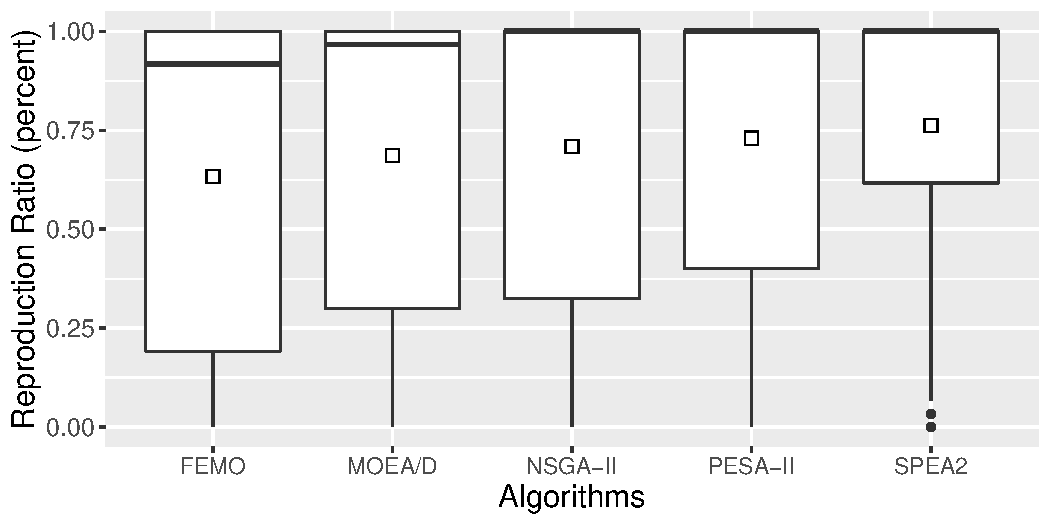
\includegraphics[width=\linewidth]{papers/moho/figures/reproduction-overall.pdf}
    % \Description{A boxplot presenting the crash reproduction ratio of the different algorithms when using MO-HO.}
    \caption{Crash reproduction ratio (out of 30 executions) of \moho algorithms.  The upper and lower edge of each box present the upper and lower quartile, respectively. ($\square$) denotes the arithmetic mean and (---) is the median.}
    \label{fig:eval:results-rq1-overall}
\end{figure}

Figure \ref{fig:eval:results-rq1-overall} presents the crash reproduction ratio of the MOEAs applied to our \moho framework. For this analysis, we consider the number of times (in percentage) each MOEAs could reproduce a given crash across 30 runs and using a search budget of five minutes. On average (the squares in Figure \ref{fig:eval:results-rq1-overall}), the best algorithm for \moho is  \textit{SPEA2}, with an average and median of $76\%$ and $100\%$ of successful reproductions, respectively. \textit{SPEA2} is Followed by \textit{PESA-II}, \textit{NSGA-II}, and \textit{MOEAD}. Also, this figure shows that the first quartile of the crash reproduction ratio of \textit{SPEA2} is, at least, about 25\% higher than other MOEAs.

According to Friedman's test, the differences in reproduction ratios are statistically significant ($p$-value $\leq$ $0.05$).
This means that some MOEAs are significantly better than others within our \moho framework.  For completeness, Table~\ref{tab:internal-assessment} reports the
ranking produced by the Friedman test. To better understand for which
pairs of MOEAS the statistical significance holds, we applied the post-hoc Conover's procedure for the pairwise comparison. The results of the comparison are also reported in Table~\ref{tab:internal-assessment}.
According to this table, the best-performing algorithm is \moho + \textit{SPEA2}, which has a significantly higher crash reproduction ratio compared to other \moho algorithms. The next algorithms are \moho + \textit{PESA-II} and \moho + \textit{NSGA-II}. These two algorithms are significantly better than \moho + \textit{MOEAD} and \moho + \textit{FEMO}. Finally, the worst algorithm in terms of crash reproduction is \textit{FEMO}, which is significantly worse than other MOEAs.


\textbf{Summary (RQ$_1$). } \textit{\moho + \textit{SPEA2} achieved the highest performance in terms of crash reproduction ratio compared to \moho + other MOEAs. 
The next best-performing MOEAs, in terms of crash reproduction, are \textit{PESA-II} and \textit{NSGA-II}.
}

\subsection{Crash Reproduction (RQ2)} 
\label{sec:results:rq2}

\begin{figure*}[t]
    \centering
    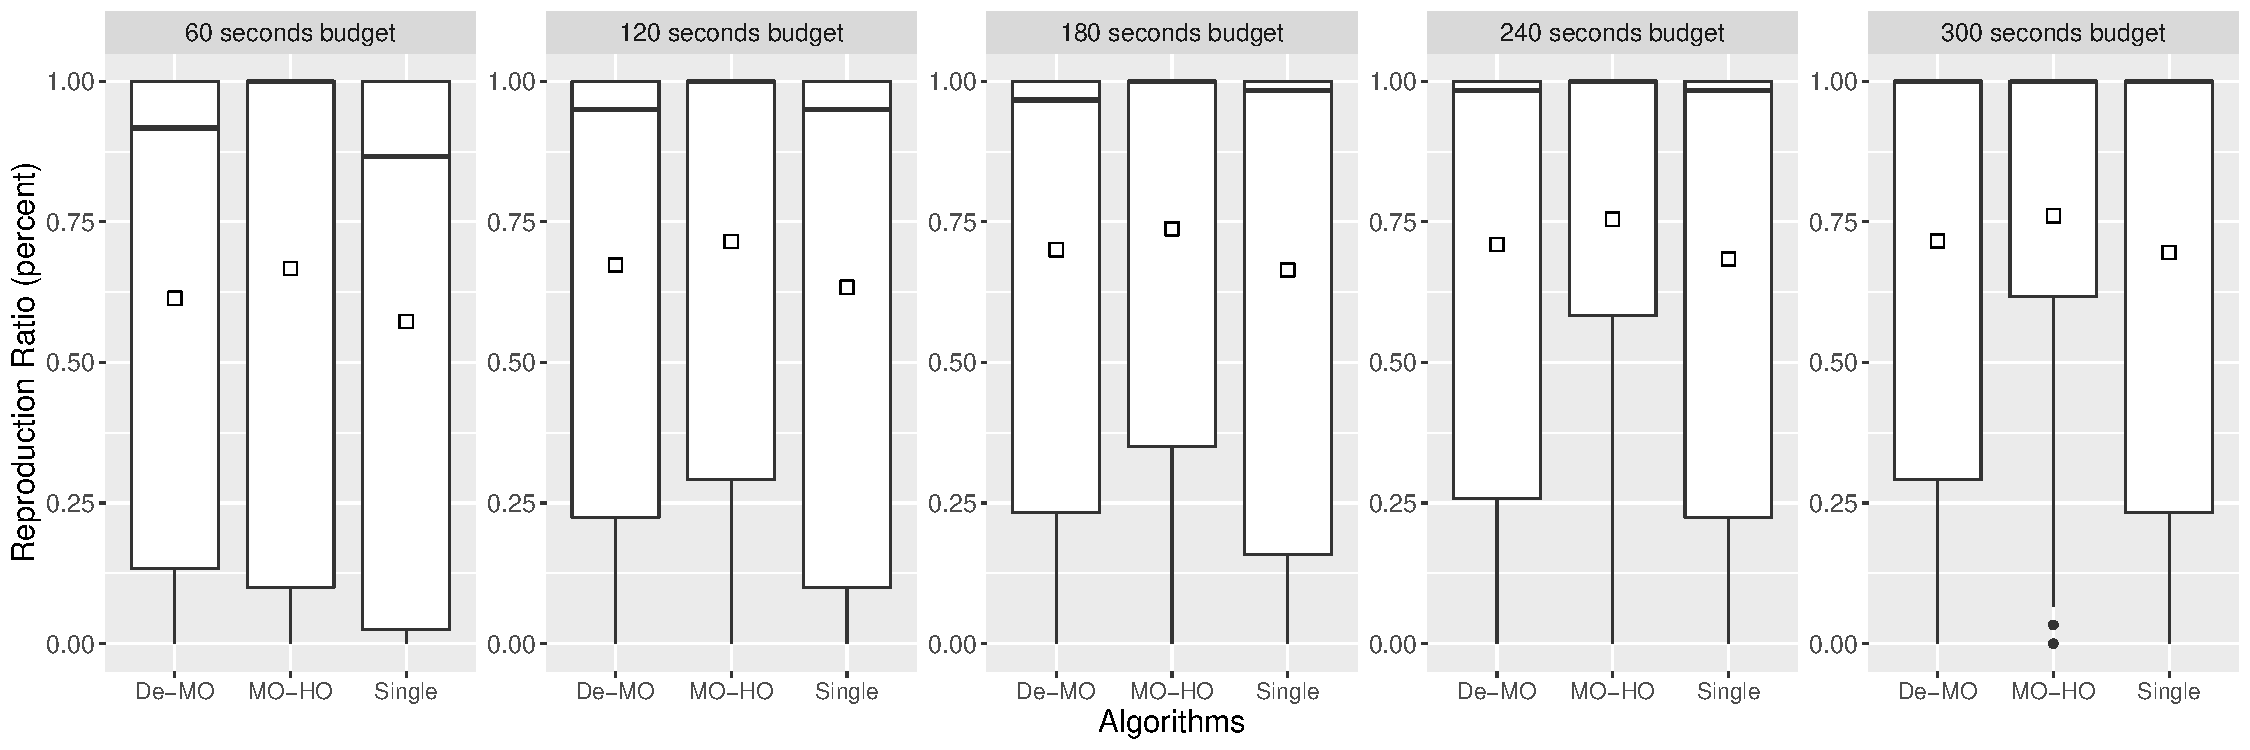
\includegraphics[width=\linewidth]{papers/moho/figures/rq2-reproduction-overall.pdf}
    % \Description{A boxplot presenting the crash reproduction ratio of MO-HO, Single and De-MO for five different time budgets.}
    \caption{Crash reproduction ratio (out of 30 executions) of \moho against state-of-the-art in five different time intervals.  ($\square$) denotes the arithmetic mean and (---) is the median.}
    \label{fig:eval:reproduction-rq2}
\end{figure*}

\begin{figure}[t]
    \centering
    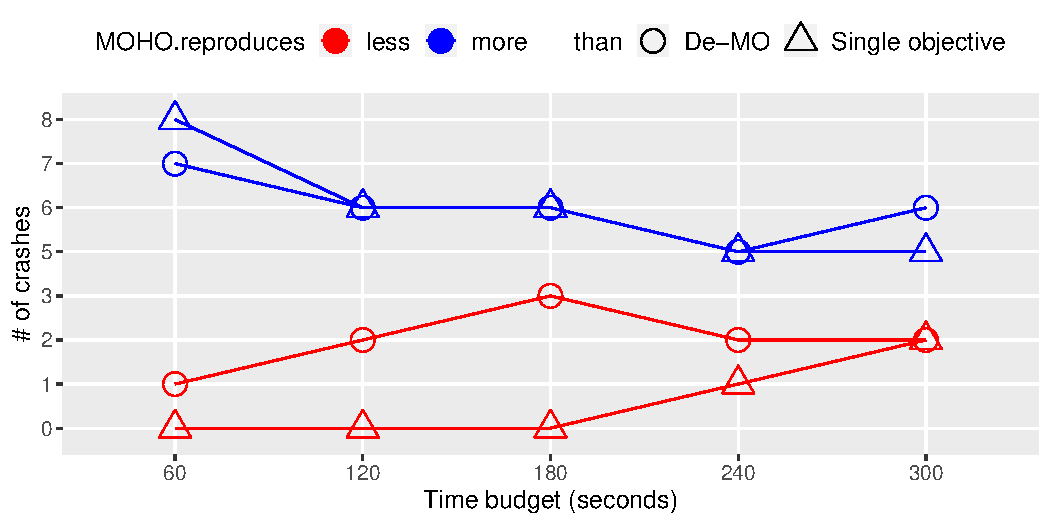
\includegraphics[width=\linewidth]{papers/moho/figures/rq2-reproduced-crashes.pdf}
    % \Description{A graph presenting the number of crashes reproduced only by MO-HO, Single, or De-MO for five different time budgets.}
    \caption{Number of reproduced crashes only by \moho or only by one of the state-of-the-art algorithms.}
    \label{fig:eval:results-rq2}
\end{figure}

Figure \ref{fig:eval:reproduction-rq2} depicts the crash reproduction ratio of the best-performing \moho configuration (i.e., with \textit{SPEA2}), \SGGA, and \decomposition at five time intervals (search budgets). As indicated in this figure, the average crash reproduction ratio of \moho is higher than other algorithms at all of the time intervals. Also, the median crash reproduction ratio for this algorithm is always 100\%. Furthermore, the maximum improvement achieved by \moho with the five-minutes search budget is in \textit{XWIKI-14599} (with 100\% improvement) and \textit{MATH-3b} (with 93.3\% improvement) compared to \SGGA and \decomposition, respectively. In contrast, the largest reduction in reproduction ratio by \moho (with the five-minutes budget) is in \textit{XCOMMONS-1057} (with 30\% drop) and \textit{XWIKI-13616} (with 40\% reduction) compared to \SGGA and \decomposition, respectively. We will explain the negative factors in \moho, which lead to negative results for this algorithm in some corner cases, in Section \ref{sec:results:corner}.
 
Moreover, we can see that \decomposition is the second-best algorithm in all of the time intervals. In the first 60 seconds of the crash reproduction process, on average, its crash reproduction ratio is 4\% better than \SGGA. However, in contrast to the other two algorithms, the crash reproduction ratio of this algorithm changes only slightly after the first 120 seconds. Hence, at the end of the search process, the average crash reproduction ratio of \decomposition is only 2\% better than \SGGA. In contrast, since the crash reproduction ratio of \moho keeps growing, on average, it remains more effective than \SGGA (about 10\%) even after 300 seconds. The other interesting point in Figure \ref{fig:eval:reproduction-rq2} is the first quantile of \moho. In the first 60 seconds, this value is lower than 12\%, but it grows up to 62\% after 300 seconds. This improvement is not observable in state-of-the-art algorithms.

Furthermore, \moho is more stable in crash reproduction after 300 seconds budget compared to the other algorithms. Figure 3 demonstrates that the interquartile range (i.e., the difference between first and third quartile) of crash reproduction ratio in \moho with the 300 seconds budget is 46\% smaller than the interquartile range of other algorithms (being 38.3\% for \moho, 76.6\%. for \SGGA, and  70.8\% for \decomposition).

Also, Figure \ref{fig:eval:results-rq2} shows the number of crashes, which are reproduced by \moho, but not by the state-of-the-art algorithms and vice versa in different time intervals.
As indicated in this figure, in all of the time intervals, the number of crashes that are reproduced by \moho is higher than the crashes that it cannot reproduce. In the best case (after 1 minute of search), \moho reproduces eight and seven new crashes that cannot be reproduced by \SGGA and \decomposition, respectively. In contrast, there is only one crash that can be reproduced by \decomposition and not by \moho. Also, after five minutes, \moho still reproduces more crashes than the baselines: it reproduces five and six new crashes that cannot be reproduced by \SGGA and \decomposition, respectively.

The crashes that are reproduced by \moho after five minutes but not by \SGGA are: \texttt{TIME-10b} frame 5, \texttt{XCOMMONS-\\928} frame 2, \texttt{XWIKI-14227} frame 2, \texttt{XWIKI-14475} frame 1, and \texttt{XWIKI-14599} frame 1. And the crashes that are reproduced by \moho after five minutes but not by \decomposition are: \texttt{MOCKITO-16b} frame 4, \texttt{TIME-5b} frame 3, \texttt{XWIKI-13377} frame 3, \texttt{XWIKI-14227} frame 2, \texttt{MATH-3b} frame 1, and \texttt{MOCKITO-10b} frame 1.

Figure \ref{lst:moho:stacktracexwiki} shows the crash's stack trace reported in the issue \texttt{X\-WI\-KI-14227}. \moho is the only approach that can reproduce the first two frames of this stack trace. Here, the target method is \texttt{useMainStore} (Figure \ref{lst:xwikiframe2}), which does not have any input argument. Hence, to reproduce this crash, the crash reproducing test generated by \moho (depicted in Figure \ref{lst:generatedtest}) should invoke specific methods (\eg \texttt{setWiki}, \texttt{setWikiId}) to set different local variables in the \texttt{xwikiContext0} object, and then, pass this object to the class under test (here, \texttt{Acti\-vi\-ty\-Stream\-Con\-fi\-gu\-ra\-tion}). Since the crash reproducing  test case generated by \moho does not add any plugin to the \texttt{xWiki0} object, the execution of this test indeed leads to a \texttt{NullPointerException} thrown at line 5619 of the \texttt{getPlugin} method in Figure \ref{lst:xwikiframe1}.
Generating such a specific test case requires a search process with high exploration ability, which can generate diverse test cases.

We do note that \SGGA cannot even generate a test case covering the target line (line 85 of the \texttt{useMainStore} method). However, \decomposition can cover the target line thanks to more test generation diversity delivered by the application of multi-objectivization.

\begin{figure}[t]
    \begin{lstlisting}[numbers=left,
        firstnumber=0]
java.lang.NullPointerException: null
	at [...].XWiki.getPlugin(XWiki.java:5619)
	at [...].ActivityStreamConfiguration.useMainStore([...]:85)
    [...]
    \end{lstlisting}
    % \Description{The stack trace from the XWIKI-14227 crash, composed of a thrown NullPointerException and the list of frames describing the active stack of method calls trough which the exception propagated.}
    \caption{XWIKI-14227 crash's stack trace.}
    \label{lst:moho:stacktracexwiki}
\end{figure}

\begin{figure}[t]
    \begin{lstlisting}[numbers=left,
        firstnumber=82,
        language=Java,
        basicstyle=\footnotesize]
public boolean useMainStore(){
    XWikiContext context = contextProvider.get();
    if (context.isMainWiki()) {return false;}
    ActivityStreamPlugin plugin = (ActivityStreamPlugin) context.getWiki().getPlugin[...] context); // <-- target line 
}
    \end{lstlisting}
    % \Description{A code excerpt of the useMainStore method mentioned in the XWIKI-14227 crash.}
    \caption{Method \texttt{useMainStore} appears in the second frame of the \texttt{XWIKI-14227} crash's stack trace.}
\label{lst:xwikiframe2}
\end{figure}
    
\begin{figure}[t]
    \begin{lstlisting}[numbers=left,
            firstnumber=5617,
            language=Java,
            basicstyle=\footnotesize]
public XWikiPluginInterface getPlugin([...]){
    XWikiPluginManager plugins = getPluginManager();
    Vector<String> pluginlist = plugins.getPlugins();
    [...]
}
    \end{lstlisting}
    % \Description{A code excerpt of the getPlugin method mentioned in the XWIKI-14227 crash.}
    \caption{Method \texttt{getPlugin} appears in the first frame of the \texttt{XWIKI-14227} crash's stack trace.}
    \label{lst:xwikiframe1}
\end{figure}
            
    
\begin{figure}[t]
    \begin{lstlisting}[numbers=left,
            firstnumber=1,
            language=Java,
            basicstyle=\footnotesize]
public void test0()  throws Throwable  {
    ActivityStreamConfiguration ac0 = new ActivityStreamConfiguration();
    XWikiContext xWikiContext0 = new XWikiContext();
    XWiki xWiki0 = new XWiki();
    xWikiContext0.setWiki(xWiki0);
    xWikiContext0.setWikiId("4~YRlfI>.U{ib");
    Provider<XWikiContext> provider0 = (Provider<XWikiContext>) mock([...]);
    doReturn(xWikiContext0).when(provider0).get();
    Injector.inject(ac0,[...], "contextProvider", (Object) provider0);
                    
    // Undeclared exception!
    ac0.useMainStore();
}
    \end{lstlisting}
    % \Description{A code excerpt of the crash-reproducing test case generated by MO-Ho for the second frame of the XWIKI-14227 crash's stack trace.}
    \caption{Crash-reproducing test case generated by \moho for the XWIKI-14227 crash.}
    \label{lst:generatedtest}
\end{figure}
    

Moreover, \SGGA and \decomposition reproduces two crashes that cannot be reproduced by \moho after five minutes. We will analyze these corner cases later in Section~\ref{sec:results:corner}.

In addition, after five minutes of crash reproduction, \decomposition reproduced six crashes, which are not reproduced by \SGGA. Still, there are more crashes (seven) that can be reproduced by \SGGA but not by \decomposition. This result shows that despite the new crashes reproduced by \decomposition, this algorithm was counter-productive with respect to the total number of reproduced crashes. 

 
\textbf{Summary (RQ$_2$). }
\textit{On average, \moho has the highest crash reproduction ratio independently from the search budgets. %The biggest improvement achieved by \moho for the crash reproduction ratio is 100\% and 93.3\% against \SGGA and \decomposition, respectively. Also, \decomposition effectiveness on the crash reproduction had been reduced after the first 2 minutes, while \SGGA and \moho continue to reproduce more crashes compared to \decomposition. Moreover, on the contrary with state-of-the-art algorithms, The lower quantile of crash reproduction ratio in \moho improved dramatically for about 50\%. Finally, we observed that \moho reproduces more crashes compared to other algorithms in all of the time intervals. In contrast, the total number of reproduced crashes by \decomposition, in the majority of runs, is less than \SGGA.
}

\subsection{Efficiency (RQ3)}
\label{sec:results:rq3}

\begin{figure}[t]
    \centering
    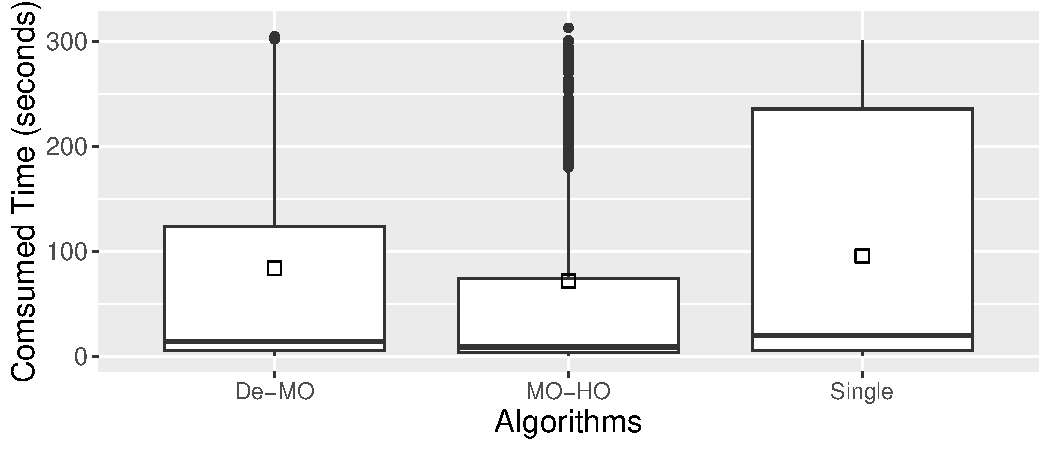
\includegraphics[width=\linewidth]{papers/moho/figures/time-overall.pdf}
    % \Description{A boxplot presenting the budget consumption in seconds fo De-MO, MO-HO, and Single.}
    \caption{Overall budget consumption in seconds (log. scale). ($\square$) denotes the arithmetic mean and (---) is the median.}
    \label{fig:eval:results-rq2-overall}
\end{figure}


Figure \ref{fig:eval:results-rq2-overall} shows the time (in seconds) needed by the \moho and the state-of-the-art algorithms to successfully reproduce the crashes in our benchmark.
On average, the fastest algorithm is \moho, with an average search time of 71 seconds per crash replication. The median of its running time is lower than 10 seconds. The second fastest algorithm is \decomposition that, on average, uses 84 seconds to reproduce the crashes. The slowest algorithm is \SGGA, which demands, on average, about 100 seconds. 

Moreover, the biggest improvements achieved by \moho in terms of efficiency are for \textit{XWIKI-14599}, in which \moho requires only 3\% of the time required by \SGGA to achieve crash reproduction, and \textit{MATH-3b}, in which \moho requires only 7\% of the time required by \decomposition to finish the crash reproduction task.
However, the biggest efficiency losses by \moho are in \textit{MATH-81b} with 45 seconds drop (15\% of time budget) and \textit{  XRENDERING-481} with 145 seconds drop (48\% of time budget) compared to \SGGA and \decomposition, respectively.

\begin{table}[t]
    \centering
    \caption{Pairwise comparison of the budget consumption with a small (S), medium (M), and large (L) effect size $\textit{\^{A}}_{12} < 0.5$ and a statistical significance $<0.05$.}
    \label{tab:efficiency}
    % \begin{smaller}
    \begin{tabular}{ l | c c c | c c c | c c c }
\hline 
\textbf{$\#(\textit{\^{A}}_{12} < 0.5)$}&\multicolumn{3}{c}{\textbf{Single}}&\multicolumn{3}{c}{\textbf{De-MO}}&\multicolumn{3}{c}{\textbf{MO-HO}}\\ 
 & L & M & S& L & M & S& L & M & S \\ 
\hline 
\textbf{Single}&-&-&-&7&-&4&1&-&2\\ 
\textbf{De-MO}&13&7&2&-&-&-&3&2&-\\ 
\textbf{MO-HO}&35&6&2&33&10&4&-&-&-\\ 
\hline
\end{tabular}
    % \end{smaller}
\end{table}

Table \ref{tab:efficiency} compares the budget consumption of the algorithms from a statistical point of view, \ie according to the effect sizes ($\textit{\^{A}}_{12} < 0.5$) and statistical significance ($\textit{p-value} < 0.5$). According to this table, \moho is the fastest algorithm: it significantly reproduced 43 (34.6\% of crashes) and 47 (37.9\% of crashes) crashes faster than \SGGA and \decomposition, respectively. Most of these significant improvements have large effect sizes (35 against \SGGA and 33 against \decomposition). In cases that \moho improves efficiency, on average, this algorithm decreases the time required for crash reproduction by 47\% and 58\% compared to \decomposition and \SGGA, respectively. 

Furthermore, Table \ref{tab:efficiency} shows a few cases, in which \moho increases the consumed time compared to the state-of-the-art: 3 against \SGGA and 5 against \decomposition. In most of these cases (7 out of 8), the crash reproduction process needs to reproduce a crash with only one frame. Even the exceptional case is a stack trace with three frames. In contrast, in cases that \moho wins, we have many crashes with more frames (six frames, for instance). Also, this table shows that \decomposition is significantly slower than \SGGA  in 11 crashes. Meanwhile, \moho is only slow in reproducing three crashes.
Hence, our proposed algorithm reduces the cases in which the multi-objectivization search process is slower than the single objective search by 73\%.

% Furthermore, Table \ref{tab:efficiency} shows that \decomposition significantly increases the speed of \SGGA in 7 crashes (6 with large effect size), while it is significantly slower than \SGGA in one crash.
% There is no statistically significant difference between these two algorithms in the remaining (large majority of) crashes.

\textbf{Summary (RQ$_3$). }
\textit{The fastest crash reproduction algorithm is \moho with an average improvement in running time in 34.6\% of the crashes compared to the state of the art.
%On average, it achieved the highest efficiency for crash reproduction. The highest improvement achieved by \moho in reproducing a crash is 97\% and 92\% against \SGGA and \decomposition, respectively. Also, it improved the crash reproduction speed in, at least, 34.6\% of the crashes. However, there are few crashes, in which \moho is slower than other algorithms. By analyzing these cases, we can see that in most of them (7 out of 8), the crash reproduction process needs to reproduce only one frame.
}


\subsection{Corner Cases Analysis}
\label{sec:results:corner}

Despite the notable improvements achieved by \moho, there are few specific cases, in which \SGGA or \decomposition outperform \moho. For instance, in Section \ref{sec:results:rq2}, \SGGA and \decomposition reproduce two crashes that are not reproduced by \moho. Also, we observed in Section \ref{sec:results:rq3} that the efficiency of these two algorithms is higher than \moho in 8 crashes.

To understand why \moho is counter-productive in a few cases, we performed a manual analysis to analyze the factors in \moho that negatively impact the crash reproduction process. Results of our analysis point to two adverse factors: \textbf{extra overhead in calculating the objectives (fitness evaluation)} and \textbf{helper-objectives misguidance}.



\begin{figure}[t]
    \begin{lstlisting}[numbers=left,
        firstnumber=0]
java.lang.ArrayIndexOutOfBoundsException: 2
    at org.apache.commons.math.linear.BigMatrixImpl.operate(BigMatrixImpl.java:997)
    \end{lstlisting}
    % \Description{The stack trace from the MATH-98b crash, composed of a thrown ArrayIndexOutOfBoundsException and the list of frames describing the active stack of method calls trough which the exception propagated.}
    \caption{\texttt{MATH-98b} crash's stack trace \cite{just2014defects4j}.}
    \label{lst:factor1-stacktrace}
\end{figure}


\begin{figure}[t]
    \begin{lstlisting}[numbers=left,
        firstnumber=991,
        language=Java,
        basicstyle=\footnotesize]
public BigDecimal[] operate(BigDecimal[] v) {
    final int nRows = this.getRowDimension();
    final int nCols = this.getColumnDimension();
    final BigDecimal[] out = new BigDecimal[v.length];
    for (int row = 0; row < nRows; row++) {
        ...
        out[row] = sum; // <-- target line 
    }
    ...
}
    \end{lstlisting}
    % \Description{A code excerpt of the operate method mentioned in the MATH-98b crash.}
    \caption{Method \texttt{operate} appears in the first frame of the \texttt{MATH-98b} crash's stack trace \cite{just2014defects4j}.}
    \label{lst:factor1-code}
\end{figure}


\textbf{Extra calculation in fitness evaluation. }
In some cases, crash reproduction is trivial, and the search process reproduces it in a few seconds. For instance, in \texttt{TIME-8b} \cite{just2014defects4j}, \SGGA and \decomposition reproduce the crash in about a second. The time required by \moho to reproduce this crash is three seconds (3 times more). This stems from the fact that fitness function evaluation in \moho is more time-consuming than the state-of-the-art: \SGGA and \decomposition need to calculate only the crash distance for each test case evaluation, while \moho needs to calculate the call diversity, as well. This extra calculation lengthens the search process by a couple of seconds. In these cases, the increased crash reproduction time is lower than 5 seconds, and it is negligible in practice.

\textbf{Helper-objectives misguidance. }
In some other cases, the scenario, which leads to crash reproduction, needs a simple sequence of methods calls to the target class. Still, the complexity of this scenario stems from the input arguments used for the method calls. In these cases, since crash reproduction does not need the call diversity, \textit{method sequence diversity} objective misguides the search process. Alternatively, we need another objective for method input argument diversity (\ie improves the diversity of the input arguments for method calls). Adding new helper-objectives to consider other aspects of diversity is part of our future agenda. 

As an example, let us analyze \texttt{MATH-98b} (Figure \ref{lst:factor1-stacktrace}), in which MO-HO doubled the time consumed by the crash reproduction search process against state-of-the-art. This crash concerns an \texttt{ArrayIndexOutOfBounds\-Exception} .
Also, this crash has only one frame. For reproducing this crash, the generated test case needs to instantiate a class called \texttt{BigMatrixImpl} and call a method named \texttt{operate} (Figure \ref{lst:factor1-code}) with precise input values. Method \texttt{getColumnDimension} used in \texttt{operate} returns the number of rows in the data variable, which has been set in the constructor. To reproduce this crash, the generated test case should pass an array with a size smaller than the passed size to the constructor. In this case, method argument diversity could help the search process, and the method call diversity is not helpful.
\section{Discussion}
\label{sec:discussion}

\subsection{Effectiveness and applicability}
Generally, \decomposition reproduces some crashes that cannot be reproduced by \SGGA due to its improved exploration ability, resulting from the multi-objectivization of the crash distance. However, since the decomposed objectives in this approach depend on one another (\eg the stack trace similarity is not helpful if the generated test does not throw the given type of exception), they may misguide the search process in various cases. For instance, as we saw in Section \ref{sec:results:rq2}, \SGGA reproduces six crashes that are not reproducible by \decomposition.

In contrast, \moho has three \textit{conflicting} search objectives. From the theory~\cite{jensen2004helper}, the objective function must be conflicting to increase the overall exploration ability. Our results confirm the theory: the chance of the search process getting trapped in a local optimum is lower by using \moho objectives compared to the ones used in \decomposition. As we observed in Section \ref{sec:results:rq2}, after 1 minute of search, \moho reproduces 8 and 7 crashes more than \SGGA and \decomposition, respectively. Also, it continues outperforming with larger search budgets (2, 3, 4, and 5 minutes) until the end of the search process. It reproduces 5 and 6 crashes more than \SGGA and \decomposition, respectively, while it cannot reproduce only two crashes, reproduced by the other algorithms.

Note that reproducing each crash needs a particular test case which drives the software under test to a particular state, and then, it calls a method with proper input variables. To achieve this goal, each crash reproducing test case needs to create multiple complex objects. Hence, reproducing five new crashes (4\% of crashes available in our benchmark) is a significant improvement for \moho.

\subsection{Factors in the benchmark crashes that impact the Success of \moho}
\label{sec:discussion:factors}

There are multiple factors/characteristics of the crashes in our benchmark that might impact the performance of our approach positively. We identify the following relevant factors: (1) the type of the exception (e.g., null pointer exception), (2) the size the stack frames, (3) the number of classes involved in the crashes, (4) the number of methods of the deepest class in the crash stack. To verify whether these factors influence the performance of our algorithm, we used the two-way permutation test~\cite{pesarin2010permutation}. The permutation test is a well-established non-parametric to assess the significance of factor interactions in multi-factorial analysis of variance (non-parametric ANOVA). We use a significance level $alpha$=0.05 and a very large number of iterations (1,000,000) to ensure the stability of the results over multiple executions of the procedure~\cite{pesarin2010permutation}. 

For the sake of our analysis, we considered the difference in crash reproduction rate between \moho and the baselines as the dependent variable, while the co-factors are our independent variables. According to the permutation test, the type of exception ($p$-value=0.006) and the number of crash stack frames ($p$-value=0.001) significantly impact the performance of \moho compared to Single Objective Search. We can also observe similar results when considering the improvements of \moho against \decomposition: $p$-values=$<10^{-12}$ for both exception type and the number of frames). In other words, there are certain types of exceptions and stack trace sizes for which \moho is statistically better than the state-of-the-art approaches.

From a deeper analysis, we observe that for \texttt{NullPointerExcep}-\texttt{tion} and \texttt{org.joda.time.IllegalFieldValueException}, \moho achieves a higher reproduction ratio than Single Objective Search when the stack traces contain up to three frames for \texttt{NPE} (+22\% in reproduction rate) and up to five frames for \texttt{IllegalFieldValueEx}-\texttt{ception} (+50\% in reproduction rate). Instead, for stack traces with more frames, the differences in reproduction ratio are negligible ($\pm 1\%$ on average) or negative (-10\% in reproduction ratio). Besides, \moho achieves better reproduction ratios for the following exceptions independently of the stack size: \texttt{XWikiExceptions} (+23\% on average), \texttt{UnsupportedOperationException} (+6\% on average), \texttt{MathRuntimeException} (+14\% on average).

Finally, \moho outperforms \decomposition when reproducing \texttt{NullPoin}-\texttt{terException} with 1-3 frames (+8\% on average), \texttt{ClassCastExcep}-\texttt{tion} (+8\% on average), \texttt{StringOutOfBoundsException} (+18\% with more than 2 frames, on average), 
\texttt{IllegalFieldException} (+8\% on average),
\texttt{UnsupportedOperationException} (+23\% on average),
\texttt{MockitoException} (+83\% for short traces, on average), and \texttt{MissingMethodInvocation} (+80\% on average).

\subsection{Crash reproduction cost}
In this study, we observed that since \moho increases the diversity of the generated test cases, it can dramatically improve the efficiency of crash reproduction. This algorithm significantly improved the speed of the search process in more than 36\% of crashes compared to \SGGA and \decomposition. In cases in which \moho had a significant impact, it improves the crash reproduction speed by more than 47\%.

Our prior study (Chapter 2) suggested 5 minutes as the search budget because the search process cannot reproduce more after 5 minutes. However, we observed that despite the high efficiency of \moho, this algorithm continues to reproduce more crashes in the second half of the time budget. Section \ref{sec:results:rq2} shows that \moho keeps increasing the crash reproduction ratio even in the last minutes of the search process, while the previous multi-objectivization approach (\decomposition) changes only slightly after the first 2 minutes of crash reproduction. Hence, increasing the search budget for \moho can lead to a higher crash reproduction ratio.


\subsection{Extendability}

The improvement achieved by the proposed helper-objectives shows the impact of suitable objectives on increasing the diversity of the generated test cases and result in improving the effectiveness and efficiency of the crash reproduction search process. Hence, we hypothesize that this approach can be extended by adding new relevant helper-objectives.
\section{Threats to validity}
\label{sec:threats}


\textbf{Internal validity.}
We cannot ensure that our implementation of \botsing is without bugs. However, we mitigated this threat by testing our tool and manually analyzing some samples of the results. We used a previously defined benchmark for crash reproduction, which contains 124 non-trivial crashes from six open-source projects and applications.  Moreover, we explained how we parametrized the evolutionary algorithms in Section \ref{sec:approach:setup}. We used the default values of these algorithms in the other open-source implementations like \evosuite and \textit{JMetal}. The effect of these values for crash reproduction is part of our future work. Finally, to take the randomness of the search process into account, we followed the guidelines of the related literature \cite{Arcuri2014} and executed each evolutionary crash reproduction algorithm for 30 times.


\textbf{External validity.}
We report our results for only 124 crashes introduced by \crashpack (Cahpter \ref{sec:jcrashpack:introduction}), which is an open-source crash reproduction benchmark collected from six open-source projects. However, we recall here that we cannot guarantee that our results are generalizable to all crashes. Evaluation \moho on a larger benchmark from more projects is part of our future work.


\textbf{Reproducibility.}
We provide \botsing as an open-source publicly available tool. Also, the data and the processing scripts used to present the results of this paper, including the subjects of our evaluation (inputs), the evolution of the best fitness function value in each generation of each execution, and the produced test cases (outputs), are openly available as a docker image~\cite{zenodoRP}. 

\section{Conclusion And Future Work} 

Crash reproduction can ease the process of debugging for developers. Evolutionary approaches have been successfully used to automate this process.
Existing evolutionary-based approaches use one single objective (\ie \CrashFunction) to guide the search and rely on guided genetic operators. 
Later strategies applied multi-objectivization via decomposition (\decomposition) in an attempt to improve diversity (and, therefore, exploration). However, the latter strategy may misguide the search process because the sub-objectives are not strongly conflicting.

In this study, we apply a new approach called Multi-Objectivizati\-on using Helper-Objectives (\moho) to tackle the problems of the former techniques. In \moho, multi-objectivization is performed by adding two helper-objectives that are in conflict with \CrashFunction. We evaluated \moho with five MOEAs, which are selected from different categories of multi-objective algorithms. Our results indicate that \moho is the most efficient algorithm, significantly outperforming \SGGA and \decomposition. Also, this algorithm is able to reproduce 8 and 5 more crashes in 1 and 5 minutes, respectively, compared to the state-of-the-art. Moreover, in contrast to the previous multi-objectivized crash reproduction approach (\decomposition), the crash reproduction ability of \moho increases with large search budgets (\ie above two minutes).

% The better performance over state-of-the-art methods is due to the ability of \moho to maintain a good balance between high method sequence diversity and short test length. 
We performed an additional analysis to find the correlation between the different aspects of the crashes and the ability of \moho in reproducing them. The result of this analysis shows that two factors in crashes significantly impact the performance of \moho: (i) type of exception and (ii) the number of crash stack frames.

Furthermore, we observed that \SGGA and \decomposition could outperform \moho but only in a few cases. We performed a manual analysis to characterize the negative factors leading to the adverse results in these cases. Our analysis reveals that two negative factors are at play in these cases: (i) extra calculations in fitness evaluation and (ii) helper-objectives misguidance. We also showed in Section \ref{sec:results:corner} that while the differences in \textit{extra calculations in fitness evaluation} are significant, they are often negligible in practice.

The contributions of the chapter are as follows:
\begin{compactenum}
    % \item The re-formulation of crash reproduction as a multi-objective problem with two new helper objectives (Section \ref{section:approach}).
    \item An open-source implementation of seven crash reproduction techniques (Section \ref{sec:approach:implementation}).
    \item An empirical comparison of seven search-based crash reproduction approaches (Section \ref{sec:setup}).
    \item An analysis of the benefits of multi-objectiv\-ization with helper objectives in terms of reproduction ratio and efficiency (Section \ref{sec:results}).
    \item The identification of the special situations in which \moho can be counter-productive (Section \ref{sec:results:corner}).
    \item The identification of a strong correlation between the ability of \moho in improving the efficiency and effectiveness of crash reproduction for combinations of exception types and the number of frames in the stack trace of the target crash (Section \ref{sec:discussion:factors}). 
\end{compactenum}

In our future work, we will investigate additional helper-objecti\-ves for crash reproduction. For instance, the current helper-objectiv\-es in \moho concern the test length and method sequence diversity. However, further objectives can be added, such as test input/data diversity. Increasing the number of objectives will require to evaluate their performance using different many-objective evolutionary algorithms. 
We will also analyze the evolution of the fitness values of existing and new objective to further investigate the root causes of good and bad performances of \moho and other objectives for different crashes and different MOEAs. 

Moreover, the search objectives introduced by \decomposition is only optimized by \textit{NSGA-II} MOEA. As future work, we will investigate the impact of utilizing other MOEAs for optimizing \decomposition objectives.
\chapter{Basic Block Coverage for Search-Based Crash Reproduction}



\label{section:bbc:introduction}

Various search-based techniques have been introduced to automate different white-box test generation activities (\eg unit testing \cite{fraser2012whole,Fraser2011}, system-level testing \cite{arcuri2019restful}, \etc). Depending on the testing level, each of these approaches utilizes dedicated fitness functions to guide the search process and produce a test suite satisfying given criteria (\eg line coverage, branch coverage, \etc). 
% In many criteria, the main goal is covering specific statements in the software under test \cite{McMinn2004}.
 
Fitness functions typically rely on \textit{control flow graphs (CFGs)} to represent the source code of the software under test \cite{McMinn2004}. Each node in a CFG is a \textit{basic block} of code (\ie maximal linear sequence of statements with a single entry and exit point without any internal branch), and each edge represents a possible \textit{execution flow} between two blocks.
Two well-known heuristics are usually combined to achieve high line and branch coverages: the \textit{approach level} and the \textit{branch distance} \cite{McMinn2004}. The former measures the distance between the execution path of the generated test and a target basic block (\ie a basic block containing a statement to cover) in the CFG. The latter measures, using a set of rules, the distance between an execution and the coverage of a \textit{true} or \textit{false} branch of a particular predicate in a branching basic block of the CFG.

% The \textit{approach level} is the number of uncovered control dependent basic blocks for the target basic block (\ie basic blocks which have at least one outgoing edge leading the execution path toward the target basic block and at least another outgoing edge leading the execution path away from the target basic block) between the closest covered control dependent basic block and the target basic block. The \textit{branch distance} is calculated from the predicate of the closest covered control dependent basic block, based on a set of predefined rules.

Both \textit{approach level} and \textit{branch distance} assume that only a limited number of basic blocks (\ie \textit{control dependent} basic blocks \cite{Allen:1970:CFA:800028.808479}) can change the execution path away from a target statement (\eg if a target basic block is the true branch of an conditional statement).
However, basic blocks are not atomic due to the presence of \textbf{implicit branches} \cite{borba2010testing} (\ie branches occuring due to the exceptional behavior of instructions).
%It is always possible that any basic block, lying between the starting point of the execution and the target basic block, impacts the target basic block coverage.
As a consequence, any basic block between the entry point of the CFG and the target basic block can impact the execution of the target basic block.
For instance, a generated test case may stop its execution in the middle of a basic block with a runtime exception thrown by one of the statements of that basic block. 
% Especially in modern applications, each basic block may contain multiple potential implicit branches (\eg chained method calls).
In these cases, the search process does not benefit from any further guidance from the approach level and branch distance.

Fraser and Arcuri \cite{fraser20151600} introduced testability transformation, which instruments the code to guide the unit test generation search to cover implicit exceptions happening in the class under test. However, this approach does not guide the search process in scenarios where an implicit branch happens in the other classes called by the class under test. This is because of the extra cost added to the process stemming from the calculation and monitoring of the implicit branches in all of the classes, coupled with the class under test.
For instance, the class under test may be heavily coupled with other classes in the project, thereby finding implicit branches in all of these classes can be expensive.

However, for some test case generation scenarios, like \textbf{crash reproduction}, we aim to cover a limited number of paths, and thereby we only need to analyse a limited number of basic blocks~\cite{Chen2015, Xuan2015, nayrolles2015jcharming, Rossler2013, Soltani2018a}. Current crash reproduction approaches rely on information about a reported crash (\eg stack trace, core dump \etc) to generate a \textbf{crash reproducing test case (\CRT)}
% However, some criteria aim to cover a limited number of paths, and thereby have a limited number of basic blocks. One of those criteria is \textbf{crash reproduction} \cite{Chen2015, Xuan2015, nayrolles2015jcharming, Rossler2013, Soltani2018a}. These rely on information about a reported crash (\eg stack trace, core dump \etc) to generate a \textbf{crash reproducing test case (\CRT)}. % that its execution leads to the same crash as the reported one. 
%Among these approaches, two of them use evolutionary algorithms to reproduce the crash: \recore and \evocrash.
%Both of these approaches use a single fitness function to guide the search process to reproduce a crash, given its stack trace.

%To reproduce a crash, both \evocrash and \recore need to guide the search process to cover the specific statements pointed by the given stack trace (\ie line numbers appeared in each frame of the stack trace). 
% For this guidance, both of the fitness functions rely on \textit{approach level} and \textit{branch distance}. Hence, they both suffer from the lack of guidance in cases that the involved basic blocks contain implicit branches.

Among these approaches, search-based crash reproduction \cite{Rossler2013, Soltani2018a} takes as input a \textbf{stack trace} to guide the generation process. More specifically, the statements pointed by the stack trace act as target statements for the approach level and branch distance.
Hence, current search-based crash reproduction techniques suffer from the lack of guidance in cases where the involved basic blocks contain implicit branches (which is common when trying to reproduce a crash). 

This chapter introduces a novel secondary objective called \textbf{Basic Block Coverage (\bbc)} to address this guidance problem in crash reproduction. \bbc helps the search process to compare two generated test cases with the same distance (according to approach level and branch distance) to determine which one is closer to the target statement. In this comparison, \bbc
analyzes the coverage level, achieved by each of these test cases, of the basic blocks in between the closest covered control dependent basic block and the target statement.

%To assess the impact of \bbc on both of the search-based crash reproduction techniques, we empirically compared the performance of these two approaches with and without using \bbc (4 configurations in total). 
We assessed the impact of \bbc secondary objective on two fitness functions in search-based crash reproduction:  \WS and \integ. The former guides the search process in \evocrash \cite{Soltani2018a}. The latter was introduced as one of the heuristics in the fitness function, which guides the search process in \recore \cite{Rossler2013} to reproduce a crash using the stack trace and core dump produced during the crash occurring. \integ is the only heuristic in \recore that measures the distance of the generated solution from the given stack trace and relies on approach level and branch distance more compared to \WS.
We empirically compared these two fitness functions' performance with and without using \bbc (4 configurations in total). 
We applied these four crash reproduction configurations to 124 hard-to-reproduce crashes introduced as \crashpack (Chapter \ref{sec:jcrashpack:introduction}).
We compare the performances in terms of \textit{effectiveness in crash reproduction ratio} (\ie percentage of times that an approach can reproduce a crash) and \textit{efficiency} (\ie time required by for reproducing a crash).

Our results show that \bbc significantly improves the crash reproduction ratio over the 30 runs in our experiment for respectively 5 and 1 crashes when compared to using \integ and \WS without any secondary objective. Also, \bbc helps these two fitness functions to reproduce 6 (for \integ) and 1 (for \WS) crashes that they could not be reproduced without secondary objective. 
Besides, on average, \bbc increases the crash reproduction ratio of \integ by 4\%. 
Applying \bbc also significantly reduces the time consumed for crash reproduction guided by \integ and \WS in 33 (26.6\% of cases) and 14 (13.7\% of cases) crashes, respectively, while it was significantly counter productive in only one case. In cases where \bbc has a significant impact on efficiency, this secondary objective improves the average efficiency of \integ and \WS by 40.6\% and 44.3\%, respectively.

\section{Background}
\label{section:bbc:background}

\begin{lstlisting}[frame=tb,
    caption={Method \texttt{fromMap} from XWIKI version 8.1 (collected in Chapter \ref{sec:jcrashpack:introduction})},
    label=list:fromMap,
    language=java,
    captionpos=t,
    numbers=left,
    basicstyle=\tiny,
    belowskip=-2.5em,
    float=t,
    firstnumber=402]
    public BaseCollection fromMap(Map<[...]> map, BaseCollection object){
        for (PropertyClass property : (Collection<[...]>) getFieldList()) {
            String name = property.getName();
            Object formvalues = map.get(name);
            if (formvalues != null) {
                BaseProperty objprop;
                if (formvalues instanceof String[]) {
                    [...]
                } else if (formvalues instanceof String) {
                    objprop = property.fromString(formvalues.toString());
                } else {
                    objprop = property.fromValue(formvalues);
                }
                [...]
            }}
        return object;}
  \end{lstlisting}
 
  \begin{figure}[t]
    \centering
    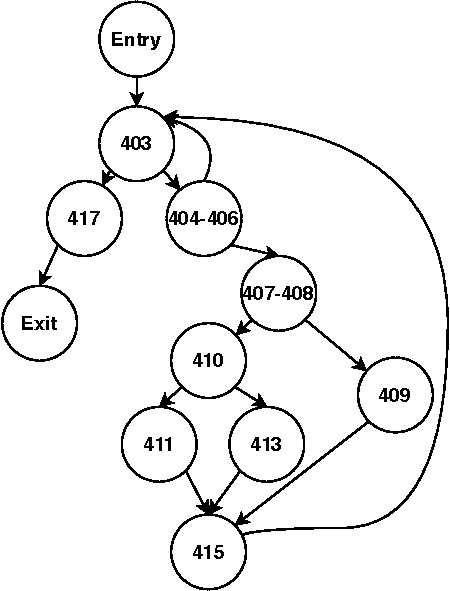
\includegraphics[width=0.35\linewidth]{papers/bbc/figures/fromMapCFG}
    
    \caption{CFG for method \texttt{fromMap}}
  \label{fig:CFG}
  \vspace{-2em}
\end{figure}

\subsection{Coverage Distance Heuristics}
\label{section:background:distance}

Many structural-based search-based test generation approaches mix the \textit{branch distance} and \textit{approach level} heuristics to achieve a high line and branch coverage~\cite{McMinn2004}. These heuristics measure the distance between a test execution path and a specific statement or a specific branch in the software under test.
For that, they rely on the coverage information of \emph{control dependent basic blocks}, \ie basic blocks that have at least one outgoing edge leading the execution path toward the \emph{target basic block} (containing the targeted statement) and at least another outgoing edge leading the execution path away from the target basic block.
As an example, Listing \ref{list:fromMap} shows the source code of method \texttt{fromMap} in XWIKI\footnote{https://github.com/xwiki}, and Figure \ref{fig:CFG} contains the corresponding CFG. In this graph, the basic block \texttt{409} is control dependent on the basic block \texttt{407-408} because the execution of line 409 is dependent on the satisfacation of the predicate at line 408 (\ie line 409 will be executed only if elements of array \texttt{formvalues} are \texttt{String}).

The \textit{approach level} is the number of uncovered control dependent basic blocks for the target basic block between the closest covered control dependent basic block and the target basic block. The \textit{branch distance} is calculated from the predicate of the closest covered control dependent basic block, based on a set of predefined rules. Assuming that the test $t$ covers only line \texttt{403} and \texttt{417}, and our target line is \texttt{409}, the approach level is 2 because two control dependent basic blocks (\texttt{404-406} and \texttt{407-408}) are not covered by $t$. The branch distance the predicate in line \texttt{403} (the closest covered control dependency of node \texttt{409}) is measured based on the rules from the establised technique \cite{McMinn2004}.

To the best of our knowledge, there is no related work studying the extra heuristics helping the combination of approach level and branch distance to improve the coverage. Most related to our work, Panichella \etal \cite{Panichella2018} and Rojas \etal \cite{rojas2015combining} introduced two heuristics called \textit{infection distance} and \textit{propagation distance}, to improve the weak mutation score of two generated test cases. However, these heuristics do not help the search process to improve the general statement coverage (\ie they are effective only after covering a mutated statement).

In this paper, we introduce a new secondary objective to improve the statement coverage achieved by fitness functions based on the approach level and branch distance, and analyze the impact of this secondary objective on \textbf{search-based crash reproduction}.

% \begin{figure}[t]
    \begin{lstlisting}[
        caption=XWIKI-13377 crash stack trace (collected in Chapter \ref{sec:jcrashpack:introduction}),
        label=lst:stacktrace,
        numbers=left,
        firstnumber=0,
        belowskip=-1.5em
        ]
java.lang.ClassCastException: [...]
    at [...].BaseStringProperty.setValue(BaseStringProperty.java:45)
    at [...].PropertyClass.fromValue(PropertyClass.java:615)
    at [...].BaseClass.fromMap(BaseClass.java:413)
    [...] (*@\label{line:bbc:lowestframe}@*)
    \end{lstlisting}
% \end{figure}

\subsection{Search-based Crash Reproduction}

After a crash is reported, one of the essential steps of software debugging is to write a \textbf{Crash Reproducing Test case (\CRT)} to make the crash observable to the developer and help them in identifying the root cause of the failure \cite{Zeller2009}. Later, this \CRT can be integrated into the existing test suite to prevent future regressions. Despite the usefulness of a \CRT, the process of writing this test can be labor-intensive and time-taking \cite{Soltani2018a}. 
Various techniques have been introduced to automate the reproduction of a crash \cite{Chen2015, Xuan2015, nayrolles2015jcharming, Rossler2013, Soltani2018a}, and search-based approaches (\evocrash \cite{Soltani2018a} and \recore \cite{Rossler2013}) yielded the best results~\cite{Soltani2018a}.


\textbf{\evocrash.}
This approach utilizes a single-objective genetic algorithm to generate a \CRT from a given stack trace and a \textit{target frame} (\ie a frame in the stack trace that its class will be used as the class under test). The \CRT generated by \evocrash throws the same stack trace as the given one up to the target frame. 
For example, by passing the stack trace in Listing~\ref{lst:stacktrace} and target frame 3 to \evocrash, it generates a test case reproducing the first three frames of this stack trace (\ie thrown stack trace is identical from line 0 to 3).

\evocrash uses a fitness function, called \WS, to evaluate the candidate test cases. \WS is the sum scalarization of three components:
\begin{inparaenum}[(i)]
    \item the \textbf{target line coverage} ($d_{s}$), which measures the distance between the execution trace and the \textit{target line} (\ie the line number pointed to by the target frame) using \textit{approach level} and \textit{branch distance};
    \item the \textbf{exception type coverage}  ($d_{e}$), determining whether the type of the triggered exception is the same as the given one; and 
   \item the \textbf{stack trace similarity}  ($d_{tr}$), which indicates whether the stack trace triggered by the generated test contains all frames (from the most in-depth frame up to the target frame) in the given stack trace.
   \end{inparaenum}

   \begin{definition}[\WS \cite{Soltani2018a}]
    For a given test case execution $t$, the \WS ($ws$) is defined as follows:
    \begin{equation}
    \small
    ws(t) = 
    \left\{
        \begin{array}{ll}
          3 \times d_{s}(t) + 2 \times max(d_{e}) + max(d_{tr}) & \textit{ if line not reached}\\
          3 \times min(d_{s}) + 2 \times d_{e}(t) + max(d_{tr}) & \textit{if line reached}\\
          3 \times min(d_{s}) + 2 \times min(d_{e}) + d_{tr}(t) & \textit{if exception thrown}
        \end{array}
      \right.
     \end{equation}
    \end{definition}
%
Where $d_{s}(t) \in [0,1]$ indicates how far $t$ is from reaching the target line and is computed using the normalized approach level and branch distance: $d_{s}(t) = \Vert approachLevel_{s}(t)  + \Vert branchDistance_{s}(t)\Vert\Vert$. 
Also, $d_{e}(t) \in \{0,1\}$ shows if the type of the exception thrown by $t$ is the same as the given stack trace ($0$) or not ($1$). Finally, $d_{tr}(t) \in [0,1]$ measures the stack trace similarity between the given stack trace and the one thrown by $t$. $max(f)$ and $min(f)$ denote the maximum and minimum possible values for a function $f$, respectively.
In this fitness function, $d_{e}(t)$ and $d_{tr}(t)$ are only considered in the satisfaction of two \textit{constraints}: (i) \textit{exception type coverage} is relevant only 
when we reach the target line and (ii) \textit{stack trace similarity} is important only when we both reach the target line and throw the same type of exception.

As an example, when applying \evocrash on the stack trace from Listing~\ref{lst:stacktrace} with the target frame 3, \WS first checks if the test cases generated by the search process reach the statement pointed to by the target frame (line 413 in class \texttt{BaseClass} in this case). Then, it checks if the generated test can throw a \texttt{ClassCastException} or not. Finally, after fulfilling the first two constraints, it checks the similarity of frames in the stack trace thrown by the generated test case against the given stack trace in Listing~\ref{lst:stacktrace}. 

% \evocrash uses a guided genetic algorithm to ensure that any test case generated during the search process contains, at least, one method call to the \textit{target method} (\ie method appeared in the target frame). In the \textbf{search initialization}, \evocrash generates random test cases that have at least one method call to the target method. Next, in each generation, \evocrash evolves the fittest test cases using \textbf{guided mutation} (a classical mutation while ensuring that the evolved test case has one or more target method calls) and \textbf{guided crossover} (a single-point crossover that keeps the target method calls in the offsprings).

\evocrash uses \textbf{guided} initialization, mutation and single-point crossover operators to ensure that the target method  (\ie the method appeared in the target frame) is always called by the different tests during the evolution process. 

% A recent study \cite{Soltani2018a} draws a comparison between all of the approaches that use only stack traces to reproduce a crash. According to its results, \evocrash outperforms other non-search-based crash reproduction approaches in terms of \textit{effectiveness in crash reproduction} and \textit{efficiency}. This study also shows the helpfulness of tests generated by \evocrash for developers during debugging. 

According to a recent study, \evocrash outperforms other non-search-based crash reproduction approaches in terms of \textit{effectiveness in crash reproduction} and \textit{efficiency}~\cite{Soltani2018a}. This study also shows the helpfulness of tests generated by \evocrash for developers during debugging. 

In this paper, we assess the impact of \bbc as the secondary objective in the \evocrash search process.


\textbf{\recore.}
This approach utilizes a genetic algorithm guided by a single fitness function, which has been defined according to the core dump and the stack trace produced by the system when the crash happened. To be more precise,  this fitness function is a sum scalarization of three sub-functions: (i) \textbf{TestStackTraceDistance}, which guides the search process according to the given stack trace; (ii) \textbf{ExceptionPenalty}, which indicates whether the same type of exception as the given one is thrown or not (identical to ExceptionCoverage in \evocrash); and (iii) \textbf{StackDumpDistance}, which guides the search process by the given core dump. 
\begin{definition}[\textit{TestStackTraceDistance} \cite{Rossler2013}]
    For a given test case execution $t$, the \textit{TestStackTraceDistance} ($STD$) is defined as follows:
    \begin{equation}
    \small
    STD(R,t) = |R| - lcp - (1-StatementDistance(s))
     \end{equation}
\end{definition}
%
Where $|R|$ is the number of frames in the given stack trace. And $lcp$ is the longest common prefix frames between the given stack trace and the stack trace thrown by $t$. Concretely, $|R| - lcp$ is the number of frames not covered by $t$. Moreover, $StatementDistance(s)$ is calculated using the sum of the approach level and the normalized branch distance to reach the statement $s$, which is pointed to by the first (the utmost) uncovered frame by $t$: $StatementDistance(s) = approachLevel_{s}(t) + \Vert branchDistance_{s}(t) \Vert$.

Since using runtime data (such as core dumps) can cause significant overhead \cite{Chen2015} and leads to privacy issues \cite{nayrolles2015jcharming}, the performance of \recore in crash reproduction was not compared with \evocrash in prior studies \cite{Soltani2018a}.
Although, two out of three fitness functions in \recore use only the given stack trace to guide the search process. Hence, this study only considers \textit{TestStackTraceDistance} $+$ \textit{ExceptionPenalty} (called \integ hereafter).

As an example, when applying \recore with \integ on the stack trace in Listing~\ref{lst:stacktrace} with target frame 3, first, \integ determines if the generated test covers the statement at frame 3 (line 413 in class \texttt{BaseClass}). Then, it checks the coverage of frame 2 (line 615 in class \texttt{PropertyClass}). After covering the first two frames by the generated test case, it checks the coverage of the statement pointed to by the deepest frame (line 45 in class \texttt{BaseStringProperty}). For measuring the coverage of each of these statements, \integ uses the approach level and branch distance. After covering all of the frames, this fitness function checks if the the generated test throws \texttt{ClassCastException} in the deepest frame.

In this study, we perform an empirical evaluation to assess the performance of crash reproduction using \integ with and without \bbc as the secondary objective in terms of \textit{effectiveness in crash reproduction} and \textit{efficiency}.

% compare the performance of the crash reproduction guided by \integ against \evocrash in terms of \textit{effectiveness in crash reproduction} and \textit{efficiency}. We also analyze the cases that one of these algorithms can achieve a better result compared to the other one. Moreover, we evaluate 

% The former utilizes a genetic algorithm guided by a single fitness function, which has been defined according to the core dump and the stack trace produced by the system when the crash happened. To be more precise,  this fitness function is a sum scalarization of two sub-functions: \integ, which guides the search process according to the given stack trace, and \textit{TestStackDumpDistance}, which guides the search process by the given core dump.
% The latter also uses a guided genetic algorithm with a single objective (called \WS hereafter), which is defined only by the given stack trace.

% Since using runtime data (such as core dumps) can cause significant overhead \cite{Chen2015} and leads to privacy issues \cite{nayrolles2015jcharming}, a recent study \cite{Soltani2018a} compares all of the crash reproduction approaches using only stack traces to fulfill this task. According to the results of this study, \evocrash outperforms other non-search-based crash reproduction approaches in terms of \textit{effectiveness in crash reproduction} (\ie percentage of times that an approach can reproduce a crash) and \textit{efficiency} (\ie time required by an approach for reproducing a crash). This study also shows the helpfulness of \CRT, generated by \evocrash, for developers during debugging. However, there is no comparison between \WS (used by \evocrash for reproducing the crash according to the stack trace) and \integ (used by \recore to reproduce the crash only by the thrown stack trace).

% However, there is no comparison between \WS (used by \evocrash for reproducing the crash according to the stack trace) and \integ (used by \recore to reproduce the crash only by the thrown stack trace).
% In this study, we perform an empirical evaluation to compare \WS against \integ in terms of \textit{effectiveness in crash reproduction} and \textit{efficiency}. We also analyze the cases that one of these algorithms can achieve a better result compared to the other one.




\section{Basic Block Coverage}
\label{section:bbc:approach}

\subsection{Motivating Example} 

During the search process, the fitness of a test case is evaluated using a fitness function, either \WS or \integ. Since the search-based crash reproduction techniques model this task to a minimization problem, the generated test cases with lower fitness values have a higher chance of being selected and evolved to generate the next generation.
One of the main components of these fitness functions is the coverage of specific statements pointed by the given stack trace. The distance of the test case from the target statement is calculated using the approach level and branch distance heuristics. As we have discussed in Section~\ref{section:background:distance}, the approach level and branch distance cannot guide the search process if the execution stops because of implicit branches in the middle of basic blocks (\eg a thrown \texttt{NullPointerException} during the execution of a basic block). As a consequence, these fitness functions may return the same fitness value for two tests, although the tests do not cover the same statements in the block of code where the implicit branching happens.

For instance, assume that the search process for reproducing the crash in Figure \ref{lst:stacktrace} generates two test cases T$_1$ and T$_2$. The first step for these test cases is to cover frame 3 in the stack trace (line \texttt{413} in BaseClass). However, T$_1$ stops the execution at line \texttt{404} due to a \texttt{NullPointerException} thrown in method \texttt{getName}, and T$_2$ throws a \texttt{NullPoint\-erException} at line \texttt{405} because it passes a null value input argument to \texttt{map}.
Even though T$_2$  covers more lines, the combination of approach level and branch distance returns the same fitness value for both of these test cases: approach level is 2 (nodes \texttt{407-408} and \texttt{410}) and branch distance is measured according to the last predicate. This is because these two heuristics assume that each basic block is atomic, and by covering line \texttt{404}, it means that lines \texttt{405} and \texttt{406} are covered, as well.

\subsection{Secondary Objective}

The goal of the Basic Block Coverage (\bbc) secondary objective is to prioritize the test cases with the same fitness value according to their coverage within the basic blocks between the closest covered control dependency and the target statement. At each iteration of the search algorithm, test cases with the same fitness value are compared with each other using \bbc. Listing \ref{list:bbc} presents the pseudo-code of the \bbc calculation. Inputs of this algorithm are two test cases T$_1$ and T$_2$, which both have the same fitness value (calculated either using \WS or \integ), as well as line number and method name of the target statement. This algorithm compares the coverage of basic blocks on the path between the entry point of the CFG of the given method and the basic block that contains the target statement (called \textit{effective blocks} hereafter) achieved by  T$_1$ and T$_2$. If \bbc determines there is no preference between these two test cases, it returns 0. Also, it returns a value $<0$ if T$_1$ has higher coverage compared to T$_2$, and vice versa. A higher absolute value of the returned integer indicates a bigger distance between the given test cases.

\begin{lstlisting}[float=t,
    caption={\bbc secondary objective computation algorithm},
    label=list:bbc,
    mathescape=true,
    frame=tb,
    numbers=left, 
    numberstyle=\tiny,
    belowskip=-2.5em,
    keywordstyle=\bfseries\em,
    keywords={,input, output, return, datatype, function, in, if, else, foreach, while, begin, end, } %add the keywords you want, or load a language as Rubens explains in his comment above.
    numbers=left,
    xleftmargin=.04\textwidth]
input: test T$_1$, test T$_2$, String method, int line
output: int
begin
    FCB$_1$ $\gets$  fullyCoveredBlocks(T$_1$,method,line);
    FCB$_2$ $\gets$  fullyCoveredBlocks(T$_2$,method,line);
    SCB$_1$ $\gets$  semiCoveredBlocks(T$_1$,method,line);
    SCB$_2$ $\gets$  semiCoveredBlocks(T$_2$,method,line);

    if (FCB$_1$ $\subset$ FCB$_2$ $\wedge$ SCB$_1$ $\subset$ SCB$_2$) $\vee$ (FCB$_2$ $\subset$ FCB$_1$ $\wedge$ SCB$_2$ $\subset$ SCB$_1$):
        return size(FCB$_2$ $\cup$ SCB$_2$) - size(FCB$_1$ $\cup$ SCB$_1$)
    else if FCB$_1$ = FCB$_2$ $\wedge$ SCB$_1$ = SCB$_2$:
        closestBlock $\gets$ closestSemiCoveredBlocks(SCB$_1$, method, line);
        coveredLines1 $\gets$ getCoveredLines(T$_1$,closestBlock);
        coveredLines2 $\gets$ getCoveredLines(T$_2$,closestBlock);
        return size(coveredLines2) - size(coveredLines1);      
    else:
        return 0;
end  
  \end{lstlisting}


In the first step, \bbc detects the effective blocks fully covered by each given test case (\ie the test covers all of the statements in the block) and saves them in two sets called \texttt{FCB$_1$} and \texttt{FCB$_2$} (lines 4 and 5 in Listing \ref{list:bbc}). Then, it detects the effective blocks semi-covered by each test case (\ie blocks where the test covers the first line but not the last line) and stores them in \texttt{SCB$_1$} and \texttt{SCB$_2$} (lines 6 and~7). 
The semi-covered blocks indicate the presence of implicit branches. Next, \bbc checks if both fully and semi-covered blocks of one of the tests are subsets of the blocks covered by the other test (line 9). In this case, the test case that covers the most basic blocks is the winner. Hence, \bbc returns the number of blocks only covered by the winner test case (line 10). If \bbc determines T$_2$ wins over T$_1$, the returned value will be positive, and vice versa. 

If none of the test cases subsumes the coverage of the other one, \bbc checks if the blocks covered by T$_1$ and T$_2$ are identical (line 11). If this is the case, \bbc checks if one of the tests has a higher line coverage for the semi-covered blocks closest to the target statement (lines 12 to 15). If this is the case, \bbc will return the number of lines in this block covered only by the winning test case. If the lines covered are the same for T$_1$ and T$_2$ (\ie \texttt{coveredLines1} and \texttt{coveredLines2} have the same size), there is no difference between these two test cases and \bbc returns value 0 (line 15).
Finally, if each of the given tests has a unique covered block in the given method (\ie the tests cover different paths in the method), \bbc cannot determine the winner and returns 0 (lines 16 and 17) because we do not know which path leads to the crash reproduction.

\textbf{Example. } 
%
When giving two tests with the same fitness value (calculated by the primary objective) T$_1$ and T$_2$ from our motivation example to \bbc with target method \texttt{fromMap} and line number 413 (according to the frame 3 of Figure \ref{lst:stacktrace}), this algorithm compares their fully and semi-covered blocks with each other. 
In this example both T$_1$ and T$_2$ cover the same basic blocks: the fully covered block is \texttt{403} and the semi-covered block is \texttt{404-406}. So, \bbc checks the number of lines covered by T$_1$ and T$_2$ in block \texttt{404-406}. Since T$_1$ stopped its execution at line 404, the number of lines covered by this test is 1. In contrast, T$_2$ managed to execute two lines (404 and 405). Hence, \bbc returns $size(coveredLines2) - size(coveredLines1) = 1$. The positive return value indicates that T$_2$ is closer to the target statement and therefore, it should have higher chance to be selected for the next generation.

\textbf{Branchless Methods. } 
%
\bbc can also be helpful for branchless methods. Since there are no control dependent nodes in branchless methods, approach level and branch distance cannot guide the search process in these cases. For instance, methods from frames 1 and 2 in Figure \ref{lst:stacktrace} are branchless. So, we expect that \bbc can help the current heuristics to guide the search process toward covering the most in-depth statement.
\section{Empirical Evaluation}
\label{sec:bbc:setup}
To assess the impact of \bbc on search-based crash reproduction, we perform an empirical evaluation to answer the following research questions:

\textbf{RQ$_1$: } \textit{What is the impact of \bbc on crash reproduction in terms of effectiveness in crash reproduction ratio?}

\textbf{RQ$_2$: } \textit{What is the impact of \bbc on the efficiency of crash reproduction?}

In these two RQs we want to evaluate the effect of \bbc on the existing fitness functions, namely \integ and \WS, from two perspectives: effectiveness on crash reproduction ratio and efficiency.

\subsection{Setup}

% \subsubsection{Implementation. }
\textbf{Implementation. }
%
Since \recore and \evocrash are not openly available, we implement \bbc in \botsing, an extensible, well-tested, and open-source search-based crash reproduction framework already implementing the \WS fitness function and the guided initialization, mutation, and crossover operators. We also implement \integ (\recore fitness function) in this tool.
\botsing relies on \evosuite \cite{Fraser2011}, an open-source search-based tool for unit test generation, for code instrumentation and test case generation by using \texttt{evosuite-client} as a dependency. 
We also implement the \integ fitness function used as baseline in this paper.

% \subsubsection{Crash selection. }
\textbf{Crash selection. }
%
We select crashes from \crashpack (Chapter \ref{sec:jcrashpack:introduction}), a benchmark containing hard-to-reproduce Java crashes.
We apply the two fitness functions with and without using \bbc as a secondary objective to 124 crashes, which have also been used in Chapter \ref{sec:model_seeding}. 
These crashes stem from six open-source projects: \textrm{JFreeChart}, \textrm{Commons-lang}, \textrm{Commons-math}, \textrm{Mockito}, \textrm{Joda-time}, and \textrm{XWiki}.
For each crash, we apply each configuration on each frame of the crash stack traces. We repeat each execution 30 times to take randomness into account, for a total number of 114,120 independent executions.
We run the evaluation on two servers with 40 CPU-cores, 128 GB memory, and 6 TB hard drive.

% \subsubsection{Parameter settings. }
\textbf{Parameter settings. }
%
We run each search process with five minutes budget and set the population size to 50 individuals, as suggested by previous studies on search-based test generation~\cite{Panichella2018}. Moreover, as recommended in prior studies on search-based crash reproduction~\cite{Soltani2018a}, we use the \textit{guided mutation} with a probability $p_m=1/n$ ($n = $ length of the generated test case), and the \textit{guided crossover} with a probability $p_c=0.8$ to evolve test cases. We do note that prior studies do not investigate the sensitivity of the crash reproduction to these probabilities. Tuning these parameters should be undertaken as future works.


\subsection{Data Analysis}

To evaluate the crash reproduction ratio (\ie the ratio of success in crash reproduction in 30 rounds of runs) of different assessed configurations (\textbf{RQ$_1$}), we follow the same procedure as Chapter \ref{sec:model_seeding}: for each crash $C$, we detect the highest frame that can be reproduced by at least one of the configurations ($r_{max}$). 
We examine the crash reproduction ratio of each configuration for crash $C$ targeting frame $r_{max}$.
Since crash reproduction data has a dichotomic distribution (\ie an algorithm reproduces a crash $C$ from its $r_{max}$ or not), we use the Odds Ratio ($OR$) to measure the impact of each algorithm in crash reproduction ratio. A value $OR > 0$ in a comparison between a pair of factors $(A,B)$ indicates that the application of factor A increases the crash reproduction ratio, while $OR < 0$ indicates the opposite. Also, a value of $OR = 0$ indicates that both of the factors have the same performance.
We apply Fisher's exact test, with $\alpha = 0.01$ for the Type I error, to assess the significance of results. 

To evaluate the efficiency of different configurations (\textbf{RQ$_2$}), we analyze the time spent by each configuration on generating a crash reproducing test case.
We do note that the extra pre-analysis and basic block coverage in \bbc is considered in the spent time.
Since measuring efficiency is only possible for the reproduced crashes, we compare the efficiency of algorithms on the crashes that are reproduced at least once by one of the algorithms. 
In executions that an algorithm failed to reproduce a crash, we assume that it reached the maximum allowed budget (5 minutes).

In this study, we use the Vargha-Delaney \^A$_{12}$ statistic \cite{vargha} to examine the effect size of differences between using and not using \bbc for efficiency.
For a pair of factors $(A,B)$ a value of \^A$_{12} > 0.5$ indicates that $A$ reproduces the target crash in a longer time, while a value of \^A$_{12} < 0.5$ shows the opposite. Also, \^A$_{12}= 0.5$ means that there is no difference between the factors.
In addition, to assess the significance of effect sizes (\^A$_{12}$), we utilize the non-parametric Wilcoxon Rank Sum test, with $\alpha = 0.01$ for the Type I error.

A replication package of this study has been uploaded to Zenodo \cite{derakhshanfar_pouria_2020_3953519}.


\begin{figure}[t]
    \subfloat[\integ\label{fig:result:overall:reproduction:integ}]{%
        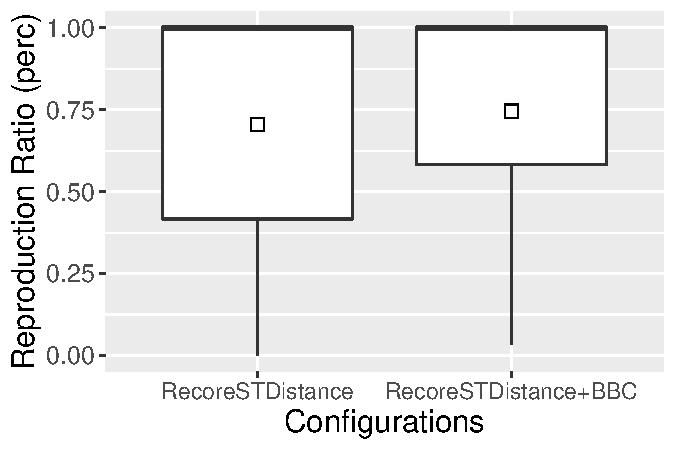
\includegraphics[width=0.45\textwidth]{papers/bbc/figures/reproduction-overall-recore.pdf}%
    }\hfil
    \subfloat[\WS\label{fig:result:overall:reproduction:ws}]{% 
        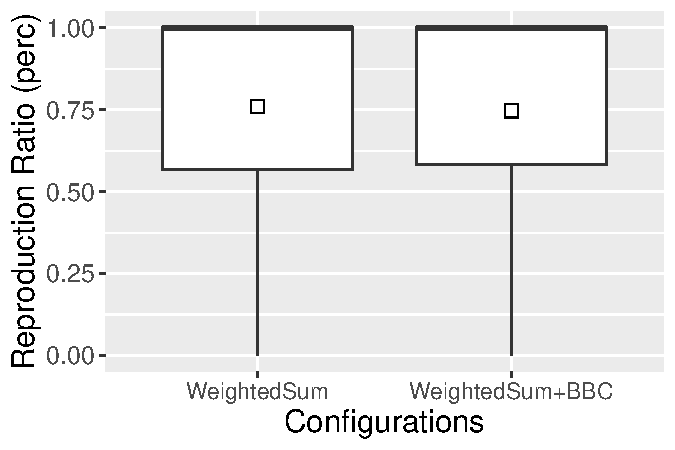
\includegraphics[width=0.45\textwidth]{papers/bbc/figures/reproduction-overall-ws.pdf}%
    }\hfil    
    \caption{Crash reproduction ratio (out of 30 executions) of fitness functions with and without \bbc. ($\square$) denotes the arithmetic mean and the bold line (---) is the median.}
    \label{fig:result:overall:reproduction}
    \vspace{-1.5em}
\end{figure}

\begin{figure}[t]
    \subfloat[\integ\label{fig:result:significance:reproduction:integ}]{%
        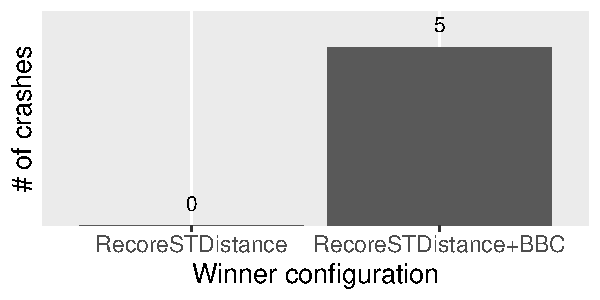
\includegraphics[width=0.45\textwidth]{papers/bbc/figures/significant-reproduction-recore.pdf}%
    }\hfil
    \subfloat[\WS\label{fig:result:significance:reproduction:ws}]{%
        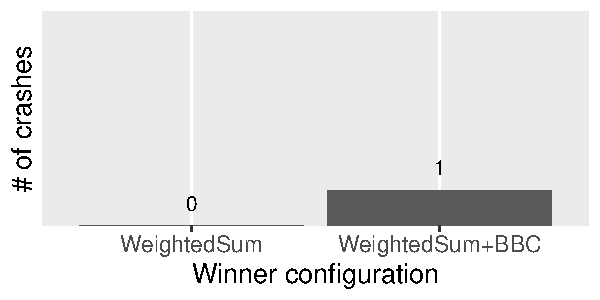
\includegraphics[width=0.45\textwidth]{papers/bbc/figures/significant-reproduction-ws.pdf}%
    }\hfil    
    \caption{Pairwise comparison of impact of \bbc on each fitness function in terms of crash reproduction ratio with a statistical significance $<0.01$.}
    \label{fig:result:significance:reproduction}
    \vspace{-1.5em}
\end{figure}

\section{Results}
\label{sec:bbc:results}

\subsubsection{Crash reproduction effectiveness (RQ$_1$)}

Figure \ref{fig:result:overall:reproduction} presents the crash reproduction ratio of the search processes guided by \integ  (Figure \ref{fig:result:overall:reproduction:integ}) and \WS (Figure \ref{fig:result:overall:reproduction:ws}), with and without \bbc as a secondary objective. This figure shows that the crash reproduction ratio of \WS improves slightly when using \bbc. However, on average, the crash reproduction ratio achieved by \integ + \bbc is 4\% better than \integ without \bbc. Also, the lower quartile of crash reproduction ratio using \integ has been improved by about 30\% by utilizing \bbc.

Figure \ref{fig:result:significance:reproduction} depicts the number of crashes, for which \bbc has a significant impact on the effectiveness of crash reproduction guided by \integ (Figure \ref{fig:result:significance:reproduction:integ}) and \WS (Figure \ref{fig:result:significance:reproduction:ws}). 
\bbc significantly improves the crash reproduction ratio in 5 and 1 crashes for fitness functions \integ and \WS, respectively. Importantly, the application of this secondary objective does not have any significant negative effect on crash reproduction. Also, \bbc helps \integ and \WS to reproduce 6 and 1 new crashes, respectively (in at least one out of 30 runs), that could not be reproduced without \bbc.

\textbf{Summary. } \bbc slightly improves the crash reproduction ratio when using the \WS fitness function. However, on average, \bbc achieves a higher improvement when used as a secondary objective with the \integ function.

\begin{figure}[t]
    \subfloat[\integ\label{fig:result:significance:efficiency:integ}]{%
        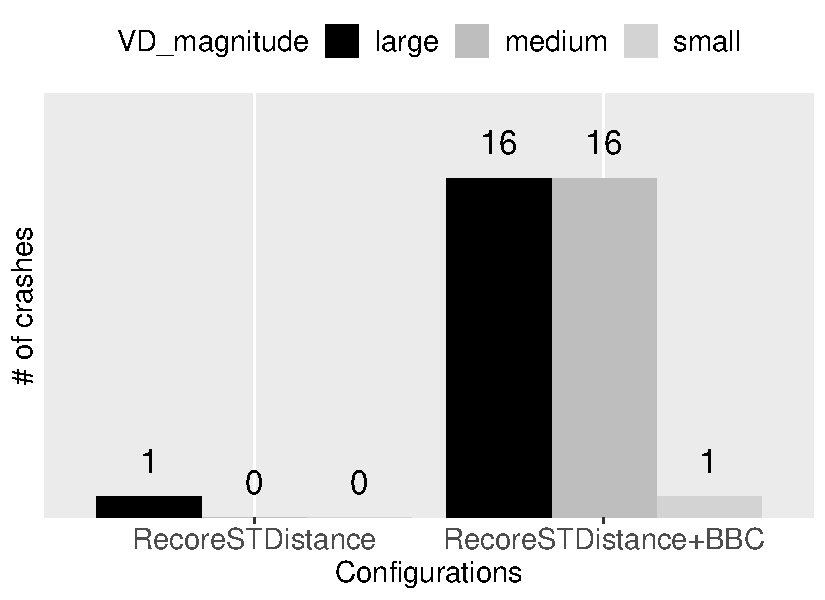
\includegraphics[width=0.45\textwidth]{papers/bbc/figures/significant-efficiency-recore.pdf}%
    }\hfil 
    \subfloat[\WS\label{fig:result:significance:efficiency:ws}]{%
        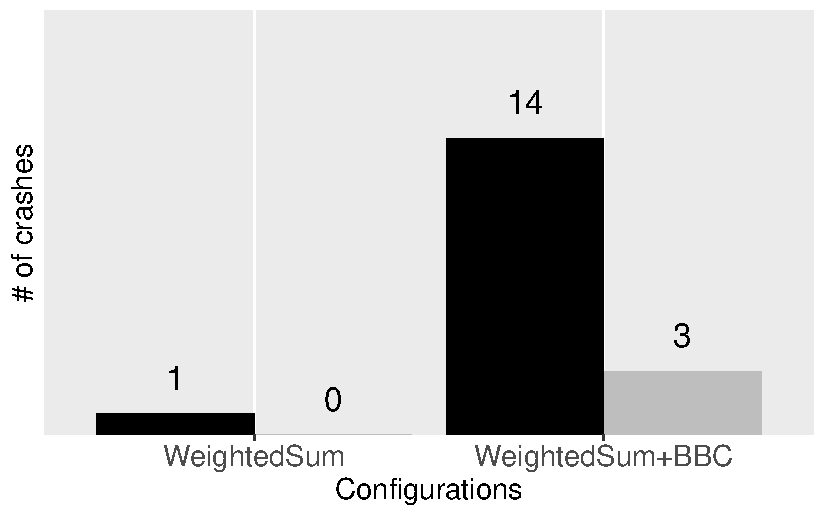
\includegraphics[width=0.45\textwidth]{papers/bbc/figures/significant-efficiency-ws.pdf}%
    }\hfil
    \caption{Pairwise comparison of impact of \bbc on each fitness function in terms of efficiency with a small, medium, and large effect size $\textit{\^{A}}_{12} < 0.5$ and a statistical significance $<0.01$.}
    \label{fig:result:significance:efficiency}
    \vspace{-1.5em}
\end{figure}
\vspace{-1em}
\subsubsection{Crash reproduction efficiency (RQ$_2$)}

Figure \ref{fig:result:significance:efficiency} illustrates the number of crashes, in which \bbc significantly affects the time consumed by the crash reproduction search process. As Figure \ref{fig:result:significance:efficiency:ws} shows, \bbc significantly improves the speed of crash reproduction guided by \WS in 17 crashes (13.7\% of cases), while it lost efficiency in the reproduction of only one crash. In cases that \bbc significantly improves the efficiency of \WS, on average, the efficiency is improved for about 40\%.
Moreover,  Figure \ref{fig:result:significance:efficiency:integ} shows that \bbc has a higher positive impact on the efficiency of the search process guided by \integ. It significantly reduces the time consumed by the search process in 33 crashes (26.6\% of cases), while it had an adverse impact on the reproduction efficiency of only one crash. In cases that \bbc significantly improves the efficiency of \integ, on average, the efficiency is improved for about 53\%.

%Furthermore, Figure \ref{fig:result:improvement:efficiency} depicts the average improvement and the effect size of cases that \bbc had a significant impact on the efficiency of the search process. 
Figure \ref{fig:result:improvement:efficiency} depicts the average improvements in the efficiency and effect sizes for crashes where the difference in the consumed budget when using \bbc or not was significant.
According to the right-side plot in Figure \ref{fig:result:improvement:efficiency:integ}, \bbc reduces the time consumed by the search process guided by \integ up to 98\% (being 40.6\% on average).
Also, the left-side plot indicates that the average effect size of differences between \integ and \integ+\bbc (calculated by Vargha-Delaney) is~0.26 (lower than 0.5 indicates that \bbc improved the efficiency).
Figure \ref{fig:result:improvement:efficiency:ws} shows that the average improvement (right-side plot) achieved by using \bbc as the second objective of \WS is 44.3\%, and the average effect size (left-side plot), in terms of the crash reproduction efficiency, is 20.5.

\textbf{Summary. } \bbc improves the efficiency of the search process with both of the crash reproduction fitness functions.

\begin{figure}[t]
    \subfloat[\integ\label{fig:result:improvement:efficiency:integ}]{%
        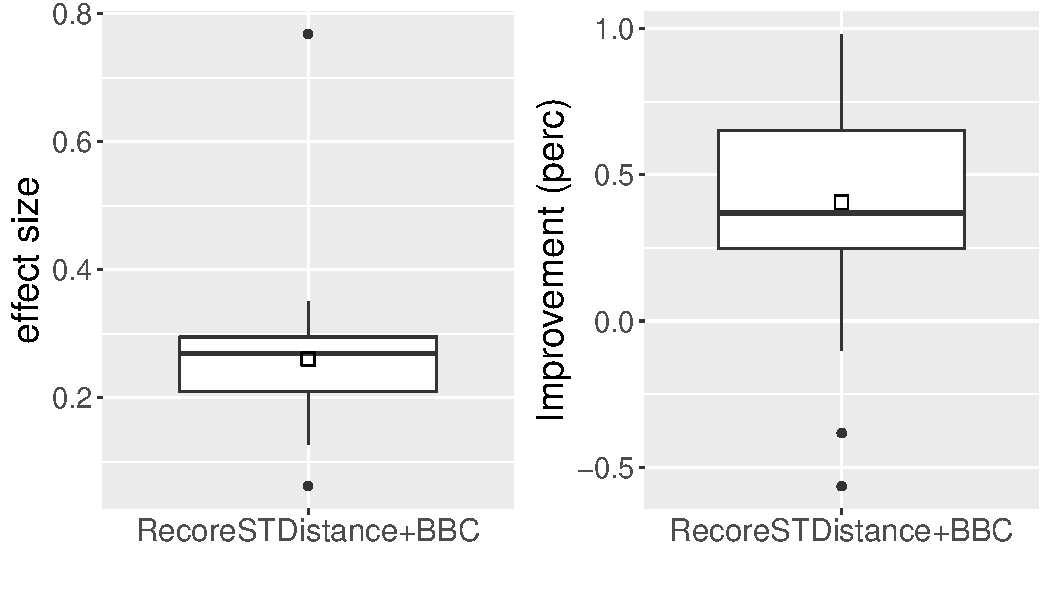
\includegraphics[width=0.5\textwidth]{papers/bbc/figures/improvement-efficiency-recore.pdf}%
    }\hfil 
    \subfloat[\WS\label{fig:result:improvement:efficiency:ws}]{%
        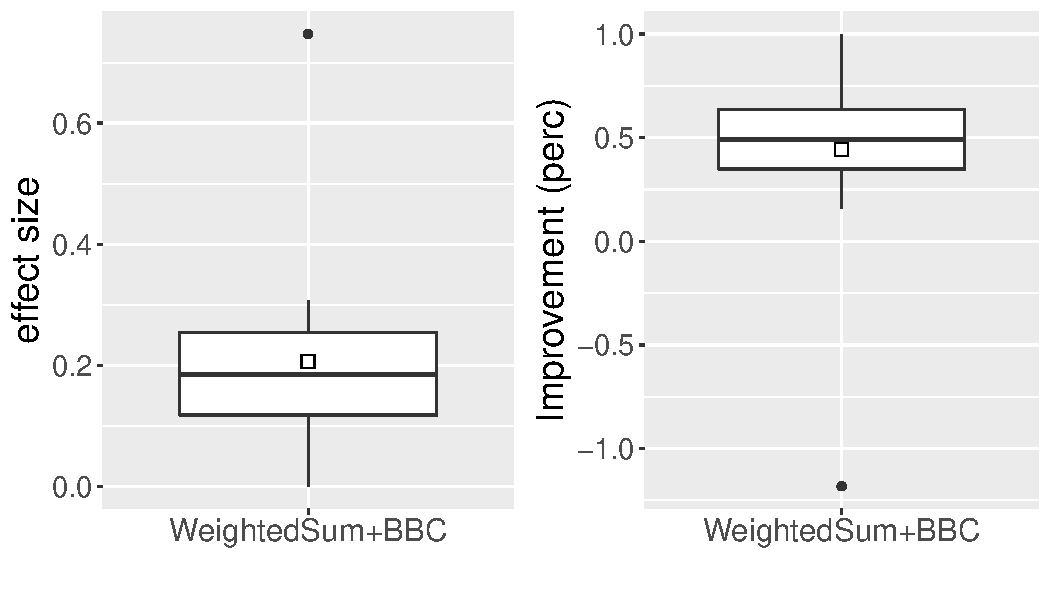
\includegraphics[width=0.5\textwidth]{papers/bbc/figures/improvement-efficiency-ws.pdf}% 
    }\hfil
    \caption{The effect size and the average improvement achieved by \bbc on each of the fitness functions in cases that \bbc makes a significant difference in terms of efficiency.}
    \label{fig:result:improvement:efficiency}
    \vspace{-2em}
\end{figure} 




\section{Discussion}
\label{sec:bbc:discussion}
Generally, using \bbc as secondary objective leads to a better crash reproduction ratio and higher efficiency in search-based crash reproduction. This improvement is achieved thanks to the additional ability to guide the search process when facing implicit branches during the search. 
Combining \bbc with \integ shows an important improvement compared to the combination of \bbc with \WS. This result was expected, since only one (out of three) component in \WS is allocated to line coverage, and thereby most parts of the fitness function do not use the approach level and branch distance heuristics. In contrast, \integ uses the approach level and branch distance to cover each of the frames in the given stack trace incrementally.

Our results show that \bbc helps the crash reproduction process to reproduce new crashes. For instance, the crash that we used in this study (XWIKI-13377) can be reproduced only by \integ + \bbc.
Considering our results, we believe that the usage of approach level and branch distance can be improved in other areas of search-based test generation (\eg unit testing) by taking the \textit{implicit branches} into account. However, it can be expensive to apply this secondary objective in cases where the search process tries to cover multiple paths. Assessing the impact of \bbc on other search-based test generation techniques is part of our future research agenda.

% We also observed in Section \ref{sec:results} that the number of crashes, in which \bbc provided a significant improvement in efficiency, is more than crashes that \bbc could significantly improve the crash reproduction ratio. This is because a particular test case, which drives the software under test to a particular state, is needed for reproducing a crash.

\section{Threats to validity.}
We cannot guarantee that our implementation of \botsing is bug-free. However, we mitigated this threat by testing our tool and manually examining some samples of the results. 
We cannot ensure that our results are generalizable to all crashes. However, we used an earlier established benchmark for crash reproduction containing 124 hard-to-reproduce crashes provoked by real bugs in a variety of open-source applications. 
Moreover, by following the guidelines of the related literature \cite{Arcuri2014}, we executed each configuration 30 times to take the randomness of the search process into account.
Finally, we provide \botsing as an open-source tool. Also, the data and the processing scripts used to present the results are available as a replication package on Zenodo\cite{derakhshanfar_pouria_2020_3953519}.

\section{Conclusion and Future Work} 
\label{sec:bbc:confut}

Approach level and branch distance are two well-known heuristics, widely used by search-based test generation approaches to guide the search process towards covering target statements and branches. These heuristics measure the distance of a generated tests from covering the target using the coverage of control dependencies. However, these two heuristics do not consider implicit branches. For instance, if a test throws an exception during the execution of a non-branch statement, approach level and branch distance cannot guide the search process to tackle this exception. In this paper, we introduced a secondary objective called \bbc to address this issue. To assess \bbc, we used it for search-based crash reproduction due to the high chance of implicit branch occurrence and the limited number of basic blocks that should be covered.
Our results show that \bbc helps \integ and \WS to reproduce 6 and 1 new crashes, respectively.
Also, \bbc significantly improves the efficiency in 26.6\% and 13.7\% of the crashes using \integ and \WS,~respectively.

In our future work, we will investigate the application of \bbc for other search-based test generation techniques (such as unit and  integration).
\vspace{-1em}
\chapter{Generating Class-Level Integration Tests Using Call Site Information}
\label{sec:cling:introduction}



%This is introduction~\cite{Jin1998}.

Search-based approaches have been applied to a variety of white-box testing activities \cite{Harman2012}, among which test case and data generation \cite{McMinn2004}. 
In white-box testing, most of the existing work has focused on the unit level, where the goal is to generate tests that achieve high structural (e.g., branch) coverage.
Prior work has shown that search-based unit test generation can achieve high code coverage~\cite{almasi2017industrial, Campos2017, Panichella2018a}, detect real-bugs~\cite{fraser20151600, Shamshiri2016}, and help developers during debugging activities~\cite{Ceccato2015, Panichella2016}.
 
Despite these undeniable results, researchers have identified various limitations of the generated unit tests~\cite{gay2015risks, Shamshiri2016, schwartz2018}. 
Prior studies have questioned the effectiveness of the generated unit tests with high code coverage in terms of their capability to detect real faults or to kill mutants when using mutation coverage. 
For example, Gay \etal~\cite{gay2015risks} have highlighted how traditional code coverage could be a poor indicator of test effectiveness (in terms of fault detection rate
 and mutation score). Shamshiri \etal~\cite{Shamshiri2016} have reported that around 50\% of faults remain undetected when relying on generated tests with high coverage. 
 Similar results have also been observed for large industrial systems~\cite{almasi2017industrial}. 

Gay \etal~\cite{gay2015risks} have observed that traditional unit-level adequacy criteria only measure whether certain code elements are reached, but not \textit{how} each element is 
covered. The quality of the test data and the paths from the covered element to the assertion play an essential role in better test effectiveness. As such, they have advocated the need 
for more reliable adequacy criteria for test case generation tools. While these results hold for generated unit tests, other studies on hand-written unit tests have further highlighted 
the limitation of unit-level code coverage criteria~\cite{wei2012branch, schwartz2018}.

%However, the search process remains mostly ignorant of how the classes under test are actually used, thus making it difficult to generate test cases involving complex parameter values or specific usages of those classes~\cite{almasi2017industrial}. Previous approaches tried to tackle this problem by retrieving information from the already existing tests (i.e., test seeding \cite{Rojas2016}) or the documentation \cite{Goffi2016}, depending on the quality of the existing tests and the availability of the documentation \cite{blasi2018, robillard2011, zhou2017}.

In this paper, we explore the usage of the integration code between coupled classes as guidance for the test generation process. The idea is that, by exercising the behavior of 
a class under test \textit{E} (the calleE) through another class \textit{R} (the calleR) calling its methods, \textit{R} will handle the creation of complex parameter values and exercise valid 
usages of \textit{E}. In other words, the caller \textit{R} might contain integration code that (1) enables the creation of better test data for the callee $E$, and (2) allows to better validate the data returned 
by \textit{E}.

Integration testing can be approached from many different angles \cite{Jin1998,Offutt2000b}.
In our case, we focus on \textbf{class integration testing} between a caller and a callee~\cite{scott1997building}.  Class integration 
testing aims to assess whether two or more classes work together properly by thoroughly testing their interactions~\cite{scott1997building}. Our idea is to  complement unit test generation
for a class under test by looking at its integration with other classes. To that end, we define a novel structural adequacy criterion that we call \textbf{Coupled Branches Coverage} (CBC), targeting specific integration 
points between two classes. Coupled branches are pairs of branches 
$\langle r, e\rangle$, with $r$ a branch of the caller, and $e$ a branch of the callee,
such that an integration test that exercises branch $r$ also exercises branch $e$.

Furthermore, we implement a search-based approach that generates integration-level test suites leveraging the CBC criterion. We coin our approach \integration
(for \underline{cl}ass \underline{in}tegration testin{\underline g}). \cling uses a state-of-the-art many-objective solver that generates test suites maximizing the number of covered coupled branches. For the guidance, \cling uses novel search heuristics defined for each pair of coupled branches (the search objectives).


We conducted an empirical study on 140 well-distributed (in terms of complexity and coupling) pairs of caller and callee classes extracted from five open-source Java projects. Our results show that \cling can achieve up to 99\% CBC scores, with an average CBC coverage of 49\% across all classes. We analyzed the benefits of the integration-level test cases generated by \cling compared to unit-level tests generated by \evosuite, the state-of-the-art generator of unit-level tests \cite{Fraser2011}. In particular, we assess whether integration-level tests generated by \cling can kill mutants and detect faults that would remain uncovered when relying on generated unit tests. 

According to our results, on average, \cling kills 7.7\% of mutants per class that remain undetected by unit tests (\evosuite) for both the caller and the callee. The improvements in mutation score are up to 50\% for certain classes, such as the \texttt{PeriodType} class in the Joda Time subject system.
Finally, we have found 32 integration faults that were detected only by the integration tests generated with \cling (and not through unit testing with \evosuite).

%In this paper, we consider only integration call type of integration between classes, although other types of integration exists between classes~\cite{Offutt2000b} (i.e., integration through external data). Furthermore, we generated integration tests for single pairs of classes, while in practice, a class can have more than one caller. However, our results are very encouraging because they show \textit{how integration-level tests based on CBC coverage complement unit-level tests generated with \evosuite in terms of test effectiveness}. Further research is needed to incorporate other types of integrations in \cling.

\textbf{Paper structure}. The remainder of this chapter is organized as follows. Section~\ref{sec:cling:background} summarizes the background and related work in the area. % test case generation and integration testing. 
Section~\ref{sec:cling:approach} defines the Coupled Branches Criteria and introduces \cling, our integration-level test case generator. Section~\ref{sec:cling:evaluation} describes our empirical study, while Section~\ref{sec:cling:results} reports the empirical results. Section~\ref{sec:cling:discussion} discusses the practical implication of our results. Section~\ref{sec:cling:threats} discusses the threats to validity. Finally, Section~\ref{sec:cling:future-conclusion} concludes the paper.





\section{Background and related work}
\label{sec:cling:background}
% !TEX root =  ../main.tex

McMinn~\cite{McMinn2004} defined search-based software testing (SBST) as \textit{``using a meta-heuristic optimizing search technique, such as a genetic algorithm, to automate or partially automate a testing task"}.
Within this realm, test data generation at different testing levels (such as \textit{unit testing}, \textit{integration testing}, \etc) has been actively investigated~\cite{McMinn2004}. This section 
provides an overview of earlier work in this area.


%As it defined by McMinn \cite{McMinn2011}, \textit{"Search-Based Software Testing is the use of a meta-heuristic optimizing search technique, such as a Genetic Algorithm, to automate or partially automate a testing task"}.
%Among these tasks, test data generation in different testing levels (such as \textit{unit testing}, \textit{integration testing}, \etc) is one of the most contributed ones \cite{McMinn2004}.
%This section outlines a summary of the previous studies about applying search-based test data generation in various levels.

\subsection{Search-based Approaches For Unit Testing}
% \acrshort{sbst} algorithms have been extensively used for unit test generation. Previous studies confirmed that thus generated tests achieve a high code coverage~\cite{Panichella2018a, Campos2018}, real-bug detection~\cite{almasi2017industrial}, and debugging cost reduction~\cite{soltani2017, Panichella2016}, complementing manually-written tests.
In Section \ref{sec:background:unit} we have explaine how the general structural-based unit testing approaches work.
We also showed an example with Listing~\ref{list:ClassA} to demonstrate how these techniques produce CFGs of the class under test and use two heuristics (called \textit{approach level} and \textit{branch distance}) to achieve a high line and branch coverage.

% From McMinn's \cite{McMinn2004} survey about search-based test data generation, we observe that most of the current approaches rely on the control flow graph (CFG) to 
% abstract the source code and represent possible execution flows. The $CFG_m=(N_m,E_m)$ represents a method\footnote{Or function in procedural programming languages.} $m$ as a directed graph of \textbf{basic blocks} of code (the nodes $N_m$), while $E_m$ is the set of the control flow edges. An edge connects a basic block $n_1$ to another one $n_2$ if the control may flow from the last statement of $n_1$ to the first statement of $n_2$.

%Following McMinn \etal's \cite{McMinn2004} survey about search-based test data generation, one of the widely used categories of approaches for automating this task is structural-based generation. These approaches use a control flow graph (CFG) to abstract the source code and represent possible execution flows.
%The \textit{control flow graph (CFG)} of method $m$ is a directed graph $CFG_m=(N_m,E_m)$ representing all paths that might be traversed through the method. In this graph, $N_m$ is the set of the \textit{basic blocks} in method $m$, and $E_m$ is the set of the control flow edges.
%A \textit{basic block} is a maximum sequence of non-branching statements in a
%method having only one entry point and one exit point.
%If one of the statements of a basic block is executed, other statements in this
%block are executed as well.
%In a CFG, an edge connects a basic block $n_1$ to another one $n_2$ if the control may flow from the last statement of $n_1$ to the first statement of $n_2$.

% Listing~\ref{list:ClassA} presents the source code of \texttt{Person}, a class representing a person and her transportation habits. A \texttt{Person} can drive home (lines 4-10), or add energy to her car (lines 12-18). The right-hand side of Figure~\ref{fig:cling:CCFG} presents the CFG of two of Person's methods, with the labels of the nodes representing the line numbers in the code. Since method \texttt{driveToHome} calls method \texttt{addEnergy}, \texttt{node 6} is transformed to two nodes, which are connected to the entry and exit point of the called method. This transformation is explained in the last paragraph of this section. 

% \begin{lstlisting}[frame=tb,
%     caption={Class \texttt{Person}},
%     label=list:ClassA,
%     language=java,
%     captionpos=t,
%     numbers=left,
%     belowskip=-2.5em,
%     float=t,
%     firstnumber=1]
% class Person{
%     private Car car = new Car();
%     protected boolean lazy = false;
%     public void driveToHome(){
%         if (car.fuelAmount < 100) {
%             addEnergy();
%         } else {
%             car.drive();
%         }   
%     }

%     protected void addEnergy(){
%         if (this.lazy) {
%             takeBus();
%         } else {
%             car.refuel();
%         }
%     }   
%     }
%   \end{lstlisting}
%   \captionof{codetype}{Type definitions}
  
 
%  \begin{figure*}[htb]
%    
%    \centering % <-- added
%\begin{subfigure}{0.25\textwidth}
%  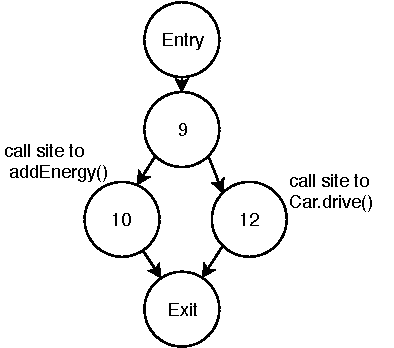
\includegraphics[width=\linewidth]{figures/driveToHome}
%  \caption{CFG of Person.driveToHome()}
%  \label{fig:driveToHome}
%\end{subfigure}\hfil % <-- added
%\begin{subfigure}{0.25\textwidth}
%  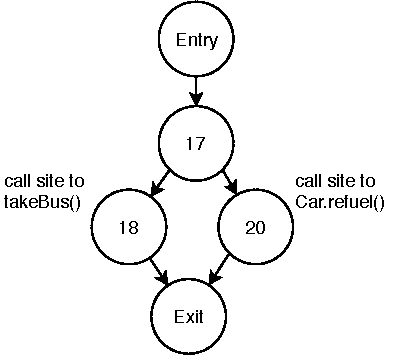
\includegraphics[width=\linewidth]{figures/refuelCar}
%  \caption{CFG of Person.addEnergy()}
%  \label{fig:refuelCar}
%\end{subfigure}\hfil % <-- added
%\begin{subfigure}{0.25\textwidth}
%  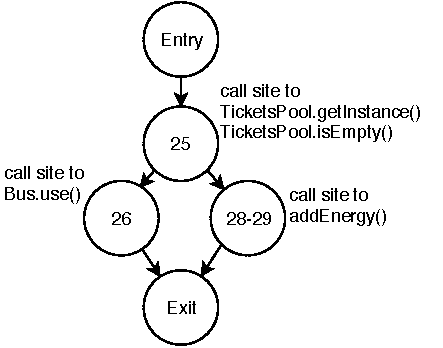
\includegraphics[width=\linewidth]{figures/takeBus}
%  \caption{CFG of Person.takeBus()}
%  \label{fig:takeBus}
%\end{subfigure}
%\caption{CFGs of methods in class $Person$}
%\label{fig:personClass}
%\end{figure*}





% Many structural-based approaches combine two common heuristics to reach a high branch and statement coverage in unit-level testing. These two heuristics  are \textit{approach level} and \textit{branch distance}.
% The \textit{branch distance} measures (based on a set of rules) the distance to \textit{satisfying} (true branch) and the distance to \textit{not satisfying} (false branch) a particular branching node in the program.
% The \textit{approach level} measures the distance between the execution path and a target node in a CFG. To describe how this heuristic measures this distance, we 
% rely on the concepts of \textbf{post-dominance} and \textbf{control dependency}~\cite{Allen:1970:CFA:800028.808479}.
% %
% %need to describe \textit{post-domination} and \textit{control dependency} first. Node $y$ in a CFG \textit{post-dominates} node $x$ if and only if every path from $x$ to the exit point of CFG contains $y$. Node $z$ in a CFG \textit{post-dominates} an edge $(x,y)$ if and only if every path from $x$ to the exit point through $(x,y)$ passes by $z$. Finally, node $y$ in a CFG is \textit{control dependent} on $x$ if $y$ post dominates one of the outgoing edges of $x$, but it does not pos-dominate node $x$ itself. 
% %
% As an example, in Figure \ref{fig:cling:CCFG}, \textit{node 8} is control dependent on \textit{node 5} and \textit{node 8} post-dominates edge $\langle 5,8\rangle$. %, but it does not post-dominate $node 5$ itself ($node 5$ can reach the exit point through $node 6$). 
% The \textit{approach level} is the minimum number of control dependencies between a target node and an executed path by a test case. 

% \medskip
In search-based unit testing, each generated test case is a sequence of method calls to a target class. This call sequence can be generated randomly, or it can be generated using existing resources. Goffi \etal \cite{Goffi2016} leverage existing documentation in this process, but for various reasons it does not allow to detect all bugs~\cite{robillard2011,blasi2018,zhou2017}.
%introduce a tool called Toradocu, which can be integrated into the test data generation process to leverage the existing documentation of the target class in this process. They show that this approach helps the test generation process to detect more exceptional bugs. However, since documentation is incomplete \cite{robillard2011}, outdated \cite{blasi2018}, or defective \cite{zhou2017}, it is not sufficient for detecting all of the bugs.
Rojas \etal~\cite{Rojas2016} collect the usages of classes in the existing test cases to generate the call sequences. To reach that goal, they need to execute each of the existing tests to find the call sequences; this may be a time taking process.

In this chapter, we analyze how a class is used/invoked by the other classes. For this purpose, we merge the Class-level Control Flow Graph (CCFG) of target callee and caller classes.


% which enriches the CFG with the calls (edges) between a target callee class and a caller class (represented using dashed lines in Figure \ref{fig:CCFG}). The CCFG is the main source we will use to generate integration tests between these two classes.


\subsection{Search-Based Approaches For Integration Testing}

Integration testing aims at finding faults that are related to the interaction between components.
We discuss existing integration testing criteria and explain the search-based approaches that use these criteria to define fitness functions for automating integration-level testing tasks.

\subsubsection{Integration testing criteria}
\label{sec:background-integ-testing-criteria}

\begin{figure}[t]
    \centering
	\includegraphics[width=0.85\linewidth]{papers/cling/figures/CCFG_new}
	\caption{Class-level CFG for class \texttt{Person}}
  \label{fig:cling:CCFG}
\end{figure}


 Jin \etal \cite{Jin1998} categorize the connections between two procedures into four levels for testing: \textit{call couplings} (level 1) occur when one procedure calls another procedure; \textit{parameter couplings} (level 2) happen when a procedure passes a parameter to another procedure; \textit{shared data couplings} (level 3) occur when two procedures refer to the same data objects; \textit{external device coupling} (level 4) happens when two procedures access the same storage device.
They introduce integration testing criteria according to the data flow graph (containing the definitions and usages of variables at the integration points) of procedure-based software. Their criteria, called \textit{coupling-based testing criteria}, require that the developed tests execute paths in the CFG of a procedure (the \textit{caller procedure}) which starts from the definition of a variable to a node (the \textit{call site}) which calls another procedure.
%The defined integration testing criteria are transformed to adapt to the object-oriented paradigm. 
%By moving from procedural-based programming to object-oriented programming, the defined integration testing criteria are transformed to adapt to this type of programming. 

Harrold \etal \cite{Harrold1994} introduced data flow testing for a single class focusing on method-integration testing. They define three levels of testing: \textit{intra-method testing}, which tests an individual method (\ie the smallest possible unit to test); \textit{inter-method testing}, in which a public method is tested that (in)directly calls other methods of the same class, and \textit{intra-class testing}, in which the various sequences of public methods in a class are tested. For data flow testing of inter-method and intra-class testing, they defined a \textit{Class-level Control Flow Graph} (CCFG). The CCFG of class \textit{C} is a directed graph $CCFG_C=(N_{Cm},E_{Cm})$ which is a composition of the control flow graphs of methods in $C$; the CFGs are connected through their call sites to methods in the same class~\cite{Harrold1994}. This graph demonstrates all paths that might be crossed within the class by calling its methods or constructors. 


Let us consider again the class $Person$ in Listing~\ref{list:ClassA}. The CCFG of class $Person$ is created by merging the CFGs of its method, as demonstrated in Figure~\ref{fig:CCFF_new}.
For example, in the CFG of the method \texttt{Person.driveToHome()}, the \textit{node 6c} is a call site to \texttt{Person.addEnergy()}. In the approach introduced by Harrold \etal \cite{Harrold1994}, they detect the def-use paths in the constructed CCFGs and try to cover those paths.
%The CCFG of a class is created by merging the CFGs of methods in this class. Following Harrold \etal's \cite{Harrold1994} approach, the first step for creating CCFG is finding all of the call sites to the methods in the same class. Next, we replace these call sites with a \emph{call node} and a \emph{return node}. Finally, we add one edge from the \emph{call node} to the entry node of the called method, and onther edges from the exit nodes of the called method to the \emph{return node}.

%\begin{figure*}[htb]
%    \centering % <-- added
%
%\begin{subfigure}{0.3\textwidth}
%    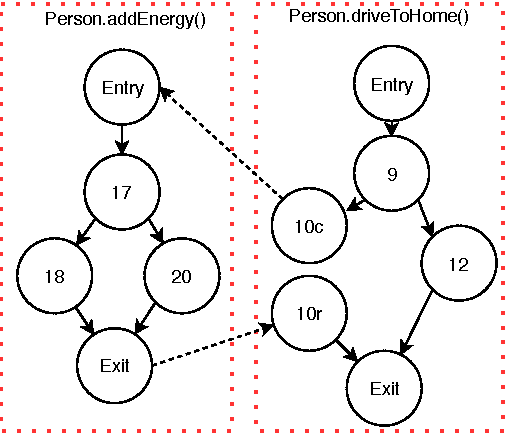
\includegraphics[width=\linewidth]{figures/merge-two-CFGs}
%    \caption{Merging methods driveToHome() and addEnergy()}
%    \label{fig:cfg-merge}
%  \end{subfigure}
%  \begin{subfigure}{0.5\textwidth}
%    \includegraphics[width=\linewidth]{figures/ACCFG}
%    \caption{Class control flow graph of A}
%    \label{fig:accfg}
%  \end{subfigure}
%
%\caption{Creating  class control flow graph of class Person}
%\label{fig:images}
%\end{figure*}



%Figure~\ref{fig:cfg-merge} shows the result of this merging of two CFGs. 
%When we merge all of the CFGs of the class $Person$, the final CCFG is shown in Figure~\ref{fig:accfg}.

A special case is represented by the polymorphic interactions that need to be tested. Alexander \etal \cite{Alexander2000, Alexander2003, Alexander2004,Alexander2010} used the data flow graph to define testing criteria for integrations between classes in the same hierarchy tree.
 %Moreover, they showed that the introduced criteria are more efficient at detecting faults than branch coverage \cite{Alexander2002a}.

 All of the mentioned approaches are using data-flow graphs to define integration testing criteria. However, generating data-flow graphs covering the def-uses involved in between classes is expensive and not scalable in complex cases. Vivanti \etal \cite{vivanti2013search} shows that the average number of def-use paths in a single class in isolation is three times more than the number of branches. By adding def-use paths between the non-trivial classes, this number grows exponentially.
 In our approach, since the number of search objectives matters (\ie too many objectives leads to the search process misguidance), we do not try to cover def-use paths. 

 Alternatively, we merge the CCFG of two classes (caller and callee class) to apply \textbf{class integration testing}. As an example, Figure \ref{fig:CCFF_new} merges two classes by linking their CFGs.
 This type of graphs is used previously for other usages. For instance, Wang \etal \cite{wang2019could} merge the CFGs of methods of classes in the dependencies of software under test to identify the dependency conflicts.
We use these merged graphs to define a new class integration testing criterion, which focuses on covering different branches in both of the classes. Our approach also considers special cases of interaction, namely inheritance and polymorphism. 


% However, in this study, we will use the CCFG of two classes to apply \textbf{class integration testing}.
% \subsubsection{Search-based approaches}

% Search-based approaches are widely used for test ordering \cite{Wang2010, Steindl2012, Hashim2005, Vergilio2012, Bansal2009, JIiang2019, Borner2009, Mariani2016, Guizzo2015, Abdurazik2009, DaVeigaCabral2010, Briand2003a, Vergilio2012}, typically with the aim of executing those tests with the highest likelihood of failing earlier on. % These studies propose a solution for ordering the integration testing of the classes in the software under test (SUT). However, they do not offer any solution for automated integration test generation.
% However, search-based approaches have rarely been used for generating integration tests. Ali Khan \etal \cite{AliKhan2013} have proposed a high-level evolutionary approach that detects the coupling paths in the data-flow graphs of classes and have used it to define the fitness function for the genetic algorithm. Then, the fitness function aids the genetic algorithm to generate tests for the detected coupling paths. Moreover, they proposed another approach for the same goal, which uses Particle Swarm Optimization \cite{Khan2014}. However, The paper does not describe the fitness function and genetic algorithm used in their approach, nor any evaluation for examining the quality of the tests generated by this approach. 
% The paper also does not check whether the tests can complement tests generated by existing search-based unit testing approaches. Besides, since objectives are defined according to the def-use paths between classes, the number of search objectives can grow exponentially, thus severely limiting the scalability of the approach (as we explained in Section \ref{sec:background-integ-testing-criteria}).

% In this study, we propose a novel approach for class integration test generation.
% Instead of using the data flow graph, which is relatively expensive to construct as it needs to find the coupling paths, we use the information available in the class call graph of the classes to calculate the fitness of the generated tests. Also, we assess our generated tests using different metrics.

% \subsection{Search-Based Approaches For Other Testing Levels}

% Arcuri \cite{Arcuri2019} proposed EvoMaster, an evolutionary-based white-box approach for system-level test generation for RESTful APIs. A test for a RESTful web service is a sequence of HTTP requests. EvoMaster tries to cover three types of targets:
%  \begin{inparaenum}[(i)]
%  \item all of the statements in the System Under Test (SUT);
%  \item all of the branches in the SUT; and
% \item different returned HTTP status codes.
% \end{inparaenum}
% Although EvoMaster tests different classes in the SUT, it does not systematically target different integration scenarios between classes.

% In contrast to EvoMaster, other approaches perform fuzzing \cite{Holler2012}, \textit{``an automated technique providing random data as input to a software system in the hope to expose a vulnerability.''} Fuzzing uses information like grammar specifications \cite{Holler2012, beyene2012, coppit2005, godefroid2008} or feedback from the program during the execution of tests \cite{Padhye2019} to steer the test generation process.
% These approaches are black-box and do not rely on any knowledge about classes in the SUT. Hence, their search processes are not guided by the integration of classes.

% Our approach performs white-box testing. It monitors the interaction between the target classes and strives to cover different integration scenarios between them.



\section{Class integration testing}
\label{sec:cling:approach}

\begin{figure}[!t]
    \centering
    \includegraphics[width=\columnwidth]{papers/cling/figures/approach.pdf}
    \caption{General overview of \integration}
    \label{fig:cling:approach}
\end{figure}

The main idea of our \underline{cl}ass \underline{in}tegration testin\underline{g} (hereinafter referred to as \cling) is to test a class by leveraging its usage by another class.
More specifically, we focus on the calls between the former, the callee ($E$), and the latter, the caller ($R$). By doing so, we benefit from the additional context setup by $R$ before calling~$E$ (\eg initializing a complex input parameter), and the additional post-processing after $E$ returns (\eg using the return value later on in $R$), thus (implicitly) adding assertions on the behavior of $E$. 

Figure \ref{fig:cling:approach} presents the general overview of \cling. \cling takes as input a pair of caller-callee $\langle R,E \rangle$ classes with at least one call (denoted \textbf{call site} hereafter) from $R$ to $E$. Since the goal of \cling is to generate test cases covering $E$ by calling methods in $R$, the first step (\circled{1}) collects the list of \textit{covering methods} in $R$ that, when called, may directly or indirectly cover statements in $E$. This list is later used  during the generation process to ensure that test cases contain calls to covering methods. The second step (\circled{2}) analyzes the CCFGs of $R$ and $E$ to identify the coupled branches between $R$ and $E$ used later on to guide the search. Finally, the generation of the test cases  (\circled{3}) uses a genetic algorithm with two additional \textit{repair} steps, ensuring that the crossover and mutation only produce test cases able to cover lines in $E$. The result is a test suite for $E$, whose test cases invokes methods in $R$ that cover the interactions between $R$ and $E$.

The remainder of this section describes our novel underlying Coupled Branches Criterion, the corresponding search-heuristics, and test case generation in \cling. 

%This study focuses on the call coupling between a class pair. We indicate these two classes as \emph{caller class} and \emph{callee class}. The \emph{caller class} must have at least one call site to \emph{callee class} (denoted \textit{interesting call sites} hereafter). The goal of \integration is covering different paths in the CFG of a given \emph{callee class} through generating tests for another given class (\emph{caller class}). The rationale behind this approach is that the generated unit tests for \textit{callee class} can be improved by some extra tests which are leveraging the usages of \textit{callee class} by the other classes.

%The main steps of \integration are demonstrated in Figure \ref{fig:cling:approach}. Before starting the search process, this approach executes two processes: \textit{Detect covering methods} and \textit{Detect branches}.
%\textit{Detect covering methods} collects methods that calling them may lead to covering the statements of \textit{callee class} (indicated as \textbf{covering methods} hereafter), and passes them to the generation processes (initialization and repair chromosomes). Also, \textit{Detect branches} collects the list of interesting edges, in both of the \textit{caller class} and \textit{callee class}, for each \textit{interesting call site}. These interesting edges are used in determining search fitness functions.
%
%In this section, we explain our new test criterion and the fitness functions driving the test generation process. Then, we detail the different steps of our novel approach.

\begin{figure}[t]
	\includegraphics[width=1.0\linewidth]{papers/cling/figures/CCFG_merge}
	\caption{Merging CCFGs of two classes: \texttt{Person} (caller) and \texttt{Car} (callee)}
  \label{fig:CCFF_new}
\end{figure}




\subsection{Coupled Branch testing criterion}

%\subsubsection{Defining the Coupled Branches} 
\label{sec:approach:coupledBranchDef}

%\begin{figure}[t]
%    \centering
%    \includegraphics[width=\columnwidth]{figures/BCCFG.pdf}
%    \caption{Class control flow graph of class B}
%    \label{fig:bccfg}
%\end{figure}

%The coupled branch criterion can be used for testing a pair of classes (\textit{caller class} and \textit{callee class}). This criterion provides an opportunity to test various combinations of certain class pairs behaviors. Since this criterion only focuses on the call couplings between these two classes, it requires to test control flow paths in the CCFG of \textit{caller class}, which reaches to an interesting call site, with the paths in the CCFG of \textit{callee class}, which starts from the entry point of the called method in that call site and ends in one of the exit points of the CCFG. For detecting these paths, we detect the \textit{interesting edges} in each of these CCFGs.

To test the integration between two classes $E$ and $R$, we need to define a coverage criterion that helps us to measure how thoroughly a test suite $T$ exercises the interaction calls between the two classes ($E$ and $R$). One possible coverage criterion would consist of testing all possible paths (\textit{inter-class path coverage}) that start from the entry node of the caller $R$, execute the integration calls to $E$ and terminate in one of the exit points of $R$. However, such a criterion will be affected by the \textit{path explosion problem}~\cite{cadar2013symbolic}: the number of paths increases exponentially with the cyclomatic complexity of $E$ and $R$, and thus the number of interaction calls between the two classes.

%\andy{Seems CBC stands for ``Coupled Branch Criterion'' or ``Coupled Branches Criterion''... we should stick to 1?}
To avoid the \textit{path explosion problem}, we define an integration-level coverage criterion, namely the Coupled Branch Criterion (CBC), where the number of coverage targets remains polynomial to the cyclomatic complexity of $E$ and $R$. More precisely, CBC focuses on call coupling between caller and callee classes. Intuitively, let $s \in R$ be a call site, i.e., a call statement to a method of the class $E$. Our criterion requires to cover all pairs of branches $ (b_r, b_e)$, where $b_r$ is a branch in $R$ that leads to $s$ (the method call), and $b_e$ is a branch of the callee $E$ that is not trivially covered by every execution of $E$. So, in the worst case, the number of coverage targets is quadratic in number of branches in the caller and callee classes.


\subsubsection{Target caller branches}
Among all branches in the caller class, we are interested in covering the branches that, when executed, always lead to the integration call site (i.e., calling the callee class). We refer to these branches as \textit{target branches} for the caller.
To understand how we determine the target branches in the caller, 
% Before introducing the formal definition of the criterion, 
let us consider the example of the caller and the callee in Figure~\ref{fig:CCFF_new}. The code for the class \texttt{Person} is reported in Figure~\ref{list:cling:ClassA}. The class \texttt{Person} contains two methods, \texttt{addEnergy()} and \texttt{driveToHome()}, with the latter invoking the former (line 6 in Listing~\ref{list:cling:ClassA}). The method \texttt{Person.addEnergy()} invokes the method \texttt{refuel()} of the class \texttt{Car} (line 16 in Listing~\ref{list:cling:ClassA}). The method \texttt{Person.driveToHome()} invokes the method \texttt{Car.drive()} (line 8 in Listing~\ref{list:cling:ClassA}). Therefore, the class \textit{Person} is the caller, while \texttt{Car} is the callee. 

Figure~\ref{fig:CCFF_new} shows an excerpt of the Class-level Control Flow Graphs (CCFGs) for the two classes. In the figure, the names of the nodes are labelled with the line number of the corresponding statements in the code of Listing~\ref{list:cling:ClassA}. Node 16 in \texttt{Person.addEnergy()} is a call site to \texttt{Car.refuel()}; it is also control dependent on nodes 5 (\texttt{Person.driveToHome()}) and 13 (\texttt{Person.addEnergy()}). Furthermore, node 16 only post-dominates branch $\langle 13,16\rangle$. Instead, the branch $\langle 5,6c\rangle$ is not post-dominated by  node 16 as covering $\langle 5,6c\rangle$ does not always imply covering node 16 as well. Therefore, the branches in the caller \texttt{Person.addEnergy()} that always lead to the callee are $B_{\mathtt{Person}}(\mathtt{Car.refuel()})=\{\langle 13,16\rangle\}$. 
%%
Hence, among all branches in the caller class (\texttt{Person} in our example), we are interested in covering the branches that, when executed, always lead to the integration call site (i.e., calling the callee class). We refer to these branches as \textit{target branches} for the caller.
 
% Considering that $CCFG_{Caller}$ is the CCFG of \textit{caller class}. The \textit{interesting} edges of interesting call site $Ics$ in this graph should have two conditions:
% \begin{inparaenum}[(i)]
%    \item it should be among the outgoing edges of nodes on which $Ics$ is control dependent; and
%    \item $Ics$ should dominate the edge.
%\end{inparaenum}
%The formal definition of interesting edges, in \textit{caller class}, for interesting call site $Ics$ is presented in Equation \ref{eq:caller_side_branches}:
%
%
%\begin{equation} \label{eq:caller_side_branches}
%    %
%    \begin{split}
%    IECaller_{Ics} = \{x : x \in E_{Caller} \wedge Pd(Ics,x) \wedge tail(x) \in CDN_{Ics}\}
%    %
%    \end{split}
%\end{equation}
%Where $E_{Caller}$ is the set of edges in $CCFG_{Caller}$; $CDN_n$ is the set of nodes on which $n$ is control dependent in graph $CCFG_{Caller}$; $Pd(n,e)$ indicates if node $n$ post dominates edge $e$; and $tail(e)$ is the tail of edge $e$ in $CCFG_{Caller}$.
\begin{definition}[\textit{Target branches for the caller}]
\textit{For a call site $s$ in $R$, the set of target branches $B_{R}(s)$ for the caller $R$ contains the branches having the following characteristics:
 \begin{inparaenum}[(i)]
    \item the branches are outgoing edges for the node on which $s$ is control dependent (\ie nodes for which $s$ post-dominates one of its outgoing branches but does not post-dominate the node itself); and
    \item the branches are post-dominated by $s$ (\ie branches for which all the paths through the branch to the exit point pass through $s$).
\end{inparaenum}
}
\end{definition}

%
%For instance, if the class \texttt{Person} in Figure \ref{list:ClassA} is the caller class and the class \texttt{Car} in Figure \ref{fig:bccfg} is the callee class. For the call site to \texttt{Car.refuel()} in node 20, node 20 is control dependent on nodes 9 and 17 but only post-dominates branch $<17,20>$, so $B_{\mathtt{Person}}(\mathtt{Car.refuel()}) = \{<17,20>\}$.

%\xavier{Can someone double check the example above? I think there was a mistake in the original one (commented below) because branch $<9,10c>$ is not post-dominated by the call site. There is a path that avoids the call site in the CCFG.}

%As we can see in Figures \ref{fig:refuelCar} and \ref{fig:takeBus}, nodes 12 and 20 are the interesting call sites. 
%These interesting call sites are control dependent on node 9 and nodes 9 and 17, respectively. Among the outgoing edges of node 9, First interesting call site (node 12) only post-dominates edge $<9,12>$. So, this edge is the only edge in set $IECaller_{12}$. Similarly, the other call site (node 20) post-dominates edges $<9,10c>$ (from outgoing edges of node 9) and $<17,20>$ (from outgoing edges of node 17). Hence, this edge is the only edge in set $IECaller_{20}$.

%Assuming that $CCFG_{Callee}$ is CCFG of \textit{callee class}. 
%The interesting edges of interesting edge $Ics$ in this graph should have two conditions:
% \begin{inparaenum}[(i)]
% \item They should be among the outgoing edges of branching nodes (nodes which has more than one outgoing edge); and 
% \item \emph they should be accessible from the entry node of the called method in $Ics$.
%\end{inparaenum}
%The formulation of interesting edges, in \textit{callee class}, for interesting call site $Ics$ is demonstrated in Equation \ref{eq:callee_side_branches}:
%
%\begin{equation} \label{eq:callee_side_branches}
%    %
%    \begin{split}
%        IECallee_{Ics} = \{x : x \in E_{Callee} \wedge |O(tail(x))| > 1 \\ 
%        \wedge \ A_{CCFG_{Callee}}(EN_{Ics},x)\}
%    \end{split}
%    %
%\end{equation}
%
%Where $EN_{Ics}$ is the entry node of called method in $Ics$; $E_{Callee}$ is the set of edges in $CCFG_{Callee}$; function $A_G(N_1,N_2)$ indicates if node $N_2$ is accessible from node $N_1$ in control flow graph $G$; and $OE(N)$ is the set of outgoing edges from node $N$.

%\andy{Do we consider it an issue that the code listing for Car is not in the paper?}
\subsubsection{Target callee branches}
Let us consider the example of Figure~\ref{fig:CCFF_new}  again. This time, let us look at the branches in the callee (\texttt{Car}) that are directly related to the integration call. In the example, executing the method call  \texttt{Car.refuel()} (node 16 of the method \texttt{Person.addEnergy()}) leads to the execution of the branching node $b8$ of the class \texttt{Car}. Hence, the set of branches affected by the interaction calls is $B_{\mathtt{Car}}(\mathtt{Car.refu}$-$\mathtt{el()}) = \{\langle b8,b9\rangle;$ $\langle b8,b10\rangle\}$. In the following, we refer to these branches as \textit{target branches} for the callee. Note that, for a call site $s$ in $R$ calling $E$, the set of target branches for the callee also  includes branches that are trivially executed by any execution of $s$. 

\begin{definition}[\textit{Target branches for the callee}]
\textit{
The set of target branches $B_{E}(s)$ for the caller $E$ contains branches satisfying the following properties: \begin{inparaenum}[(i)]
 \item the branches are among the outgoing branches of branching nodes (\ie the nodes having more than one outgoing edge); and 
 \item the branches are accessible from the entry node of the method called in $s$.
\end{inparaenum}
}
\end{definition}

%In our example, the called methods of class $Car$ (callee class) by class $Person$ (caller class) are $Car.drive()$ and $Car.refuel()$. As it demonstrated by Figure \ref{fig:bccfg}, the accessible branching nodes from the entry nodes are $b1$, $b4$, and $b6$ for $Car.drive()$ and $b8$ for $Car.refuel()$. So, the interesting edges for node 12 ($IECallee_{12}$), which calls $Car.drive()$, are outgoing edges of nodes $b1$ and $b4$: $<b1,b2>, <b1,b4>, <b4,Exit>, <b4,b5c>,<b6,b7>$, and $<b6,b8>$. In the same manner, the interesting edges for node 20 ($IECallee_{20}$), which calls $Car.refuel()$, are outgoing edges of node $b8$:  $<b8,b9>$ and $<b8,b10>$.
\subsubsection{Coupled branches}
Given the sets of target branches for both the caller and  callee, an integration test case should exercise at least one target branch for the caller (branch affecting the integration call) and one target branch for the callee (i.e., the integration call should lead to covering branches in the callee). In the following, we define pairs of target branches $(b_r \in B_{R}(s), b_e \in B_{E}(s))$ as \textit{coupled branches} because covering  $b_r$ can lead to covering $b_e$ as well. In our example of Figure~\ref{fig:CCFF_new}, we have two coupled branches: the branches $(\langle 13,16\rangle,\langle b8,b9\rangle)$ and the branches $(\langle 13,16\rangle$, $\langle b8,b10\rangle)$.

\begin{definition}[\textit{Coupled branches}]
\textit{
Let $B_{R}(s)$ be the set of target branches in the caller class $R$; let $B_{E}(s)$ be the set of target branches in the callee class $E$; and let $s$ be the call site in $R$ to the methods of $E$. The set of coupled branches $CB_{R,E}(s)$ is the cartesian product of $B_{R}(s)$ and $B_{E}(s)$:
}
\begin{equation}\label{def2}
	CB_{R,E}(s) = CB_{R,E}(s) = B_{R}(s) \times B_{E}(s)
\end{equation}
\end{definition}
%The set of \emph{coupled branches} $CB_{R,E}(s)$ for a call site $s$ from $R$ to $E$ is the product of $B_{R}(s)$ by  $B_{E}(s)$: $CB_{R,E}(s) = B_{R}(s) \times B_{E}(s)$.  

\begin{definition}\label{def3}
\textit{
Let $S=(s_1, \dots, s_k)$ be the list of call sites from a caller $R$ to a callee $E$, the set of coupled branches for $R$ and $E$ is the union of the coupled branches for the different call sites $S$: $CB_{R,E} = \cup_{s \in S} CB_{R,E}(s)$.
}
\end{definition}

%The \textit{Coupled Branches} of each interesting call site $Ics$ is the set of edge pairs which are made by combining edges in $IECaller_{Ics}$ and $IECallee_{Ics}$.
%The \textit{Coupled Branches} set is formalized in Equation \ref{eq:coupled_branches}:
%
%\begin{equation} \label{eq:coupled_branches}
%    \begin{split}
%    Coupled\_Branches_{Ics} = IECaller_{Ics} \times IECallee_{Ics}
%    \end{split}
%\end{equation}
%
%Where function $EN(m)$ gives the entry node of CFG of method $m$; $cm_x$ is the called method in call site $x$; $A_{CCFG_{Caller}}(b_1,x)$ indicates that call site $x$ is accessible from edge $e_1$ in $CCFG_{Caller}$; and $A_{CCFG_{Callee}}(EN(cm_x),e_2)$ evalauates the accesibility of edge $e_2$ from the entry node of the called method in call site $x$.
%
%In our example, as we described, node 12 is one of the interesting call sites. Its coupled branches ($Coupled\_Branches_{12}$) is the combination of edges in $IECaller_{12}$ and $IECallee_{12}$. This set contains $1 \times 6 = 6$ edge pairs. Also, the coupled branches of our second interesting call site ($Coupled\_Branches_{20}$) is the combination of edges in $IECaller_{20}$ and $IECallee_{20}$. This set contains $2 \times 2 = 4$ edge pairs.

%The set of coupled branches for a given caller and callee class is the union of the \textit{coupled branches} of the interesting call sites. The formalized definition of coupled branches of \textit{caller class} $C_1$ and \textit{callee class} $C_2$ is presented in Equation \ref{eq:coupled_branches_classes}.
%
%\begin{equation} \label{eq:coupled_branches_classes}
%    \begin{split}
%    CB_{C_1, C_2} = \{\bigcup\limits_{Ics \in I(C_1,C_2)}  Coupled\_Branches_{Ics} \}
%    \end{split}
%\end{equation}
%Where $I(C_1,C_2)$ gives the set of interesting call sites between caller class $C_1$ and callee class $C_2$.
%
%In our example, $CB_{Person, Car}$ is the union of sets $Coupled\_Branches_{12}$ and $Coupled\_Branches_{20}$.

\subsubsection{Coupled Branches Criterion (CBC)}\label{sec:approach:coupledBranchCrit}

%This criterion requires that the test suite \textit{T} covers all of the edge pairs which are indicated as coupled branches of a particular caller class and callee class. \textit{T} covers an edge pair if this test set contains at list one test case which covers both of these edges.

% Assuming that $T= \{ t_1, t_2, ..., t_n\}$ is a test suite which contains $n$ test cases. And, we want to check CBC for classes $C_1$, as the \textit{caller class}, and $C_2$ as the \textit{callee class}. Also, $I$ is the set of interesting call sites between these two classes. In this case, $T$ fulfills CBC if it coveres all of the edge pairs which are indidicated as coupled branches of call sites in $I$. This definition is formalized in Equation \ref{eq:cbc}:

% \begin{equation} \label{eq:cbc}
%     \begin{split}
%         \forall Ics \in I: \forall (e_1,e_2) \in Coupled\_Branches_{Ics} : \\
%          \exists t \in T : t \  covers \ e_1 \wedge t \ covers \ e_2
%     \end{split}
% \end{equation}

%To measure CBC of a test suite $T= \{ t_1, t_2, ..., t_n\}$ for \textit{caller class} $C_1$ and \textit{callee class} $C_2$, we use Equation \ref{eq:cbc-measure}. This equation is representing the percentage of covered \textit{coupled branches} of these two classes.
%
%\begin{equation} \label{eq:cbc-measure}
%    \begin{split}
%        \frac{|{(e_1,e_2): (e_1,e_2) \in CB_{C_1, C_2} \wedge (\exists t \in T: t \ covers \ e_1 \ and \ e_2)}|}{|CB_{C_1, C_2}|}
%    \end{split}
%\end{equation}
%
%Where $(e_n,e_m)$ is an edge pair in the \textit{coupled branches} of the given classes.
Based on the definition above, the CBC criterion requires that for all the call sites $S$ from a caller $R$ to a callee $E$, a given test suite $T$ covers all the coupled branches:
$$
CBC_{R,E} = \frac{
        \vert \{(r_i,e_i) \in CB_{R,E} \vert \exists t \in T: t \ covers \ r_i \ and \ e_i\} \vert
    }{
        \vert CB_{R,E} \vert
    }
$$
%
%As for classical branch pair coverage, achieving $100 \%$ is not always possible because the conditions in the branching nodes are in a specific situation that covering both of the edges in the edge pair is not possible. Detecting and filterin these kind of branch pairs are not easy as they need some expensive symbolic executions.
%
We do note that this formula is only relevant if there are indeed call interactions between caller and callee.
As for classical branch and branch-pair coverage, $CB_{R,E}$ may contain unreachable branch-pairs. However, detecting and filtering those incompatible pairs is an undecidable problem. Hence, in this study, we target all coupled branches.
\subsubsection{Inheritance and polymorphism}
\label{subsec:inheritance}

\begin{lstlisting}[frame=tb,
    caption={Class GreenPerson},
    label=list:ClassAPrime,
    captionpos=t,
    numbers=left,
    belowskip=-2em,
    float=t,
    language=java,
    firstnumber=1]
Class GreenPerson extends Person{
    private HybridCar car = new HybridCar();
    @override
    public void addEnergy(){
        if(this.lazy){
            takeBus();
        }else if (chargerAvailable()){
            car.recharge()
        }else{
            car.refuel();
        }
    }

    private void chargerAvailable(){
        if(ChargingStation.takeavailableStations().size > 0){
            return true;
        }
        return false;
    }
}
\end{lstlisting}

%Assuming the given \textit{caller class} and {callee class} are in the same inheritance tree. In this case, one of the classes is \textit{superclass} and the other one is a \textit{subclass} which extends \textit{superclass}. To support polymorphism by introduced criterion, we use a different procedure for finding the call sites and generating CCFG of given classes.

%A call site from a \textit{superclass} to a \textit{subclass} is the basic blocks which have a call to one of the overridden methods by \textit{subclass}. Also, a call site from a \textit{subclass} to a \textit{superclass} is the basic blocks having a call to one of the declared methods in the \textit{superclass} which is not overridden by \textit{subclass}.
  
%The CCFG of a \textit{superclass} is made by merging the CFGs of the methods which are defined in the \textit{superclass} but not overridden by \textit{subclass}. Furthermore, the CCFG of a \textit{subclass} is composed by merging the CFGs of the methods which are particularly defined or overridden by \textit{subclass}. Hence, the CFGs of inherited methods from \textit{superclass} which is not overridden by \textit{subclass} is not merged into this CCFG.

In the special case where the caller and callee classes are in the same inheritance tree, we use a different procedure to build the CCFG of the super-class and find the call sites $S$. The CCFG of the super-class is built by merging the CFGs of the methods that are not overridden by the sub-class. As previously, the CCFG of the sub-class is built by merging the CFGs of the methods defined in this class, including the inherited methods overridden by the sub-class (other non-overridden inherited methods are not part of the CCFG of the sub-class).

%As an illustration, consider that class $GreenPerson$ (Listing \ref{list:ClassAPrime}) extends class $Person$. This class represents a person who has a hybrid car. So, for adding energy to her car, she can either refuel or recharge her car (lines 7 to 11). This class overrides method $addEnergy()$ from its superclass. Also, it declares a new method named $chargerAvailable()$ which indicates if the charging station is available or it is occupied.

%As demonstrated in Figure \ref{fig:subSuperClasses}, the CFG of method $addEnergy()$ is not used in the composition of $Person$ CCFG (Figure \ref{fig:personAsSuperCCFG}). In this graph, nodes $10$ and $28-29$, which call to an overridden method, are call sites to $GreenPerson$.
% Morover, we only use the CFG of overriden method $addEnergy()$ and newly defined method $chargerAvailable()$ for creating CCFG of $GreenPerson$ (Figure \ref{fig:greenPersonCCFG}), and we do not use the other inherited methods (methods $driveToHome ()$ and $takeBus ()$) in this CCFG. In this graph node $6$, which calls a non-overriden inherited method, is call site to $Person$.

For instance, the class \texttt{GreenPerson} in Listing \ref{list:ClassAPrime}, representing owners of hybrid cars, extends class \texttt{Person} from Listing \ref{list:cling:ClassA}. For adding energy, a green person can either refuel or recharge her car (lines 7 to 11). \texttt{Green\-Person} overrides the method \texttt{Person.add\-En\-er\-gy()} and defines an additional method \texttt{Green\-Person.char\-ger\-Avai\-la\-ble()} indicating whether the charging station is available. Only those two methods are used in the CCFG of the class \texttt{Green\-Person} presented in Figure \ref{fig:greenPersonCCFG}, inherited methods are not included in the CCFG; the CCFG of the super-class \texttt{Person} does not contain the method \texttt{Person.addEnergy()}, redefined by the sub-class \texttt{GreenPerson}.

The call sites $S$ are identified according to the CCFGs, depending on the caller and the callee. If the caller $R$ is the super-class, $S$ will contain all the calls in $R$ to methods that have been redefined by the sub-class. For instance, nodes 6 and 13 in Figure \ref{fig:CCFF_new} with \texttt{Person} as caller. If the caller $R$ is the sub-class, $S$ will contain all the calls in $R$ to methods that have been inherited but not redefined by $R$. For instance, node 6 in Figure \ref{fig:greenPersonCCFG} with \texttt{GreenPerson} as caller.

\begin{figure}[!t]
    \centering
  \includegraphics[width=0.65\linewidth, angle=-90]{papers/cling/figures/GreenPerson2}
\caption{CCFG of $GreenPerson$ as subclass}
\label{fig:greenPersonCCFG}
\end{figure}
 

\subsubsection{Advantage of using CBC}
Prior works proposed to use dataflow based criteria for integration testing~\cite{Jin1998, Harrold1994,Alexander2000, Alexander2003, Alexander2004, Alexander2010}. Hence, in this section, we discuss the advantages of using CBC compared to these criteria.
CBC does not construct dataflow graphs and, consequently, calculates the coverage targets faster. CBC also requires covering additional interactions between caller and callee compared to the other criteria relying on dataflow graphs to indicate the coupling paths. As an example, assume a variable \textit{v1} defined by \textit{node 13} in method \texttt{addEnergy()} of class \texttt{Person} (Figure \ref{fig:CCFF_new}), and that is used afterward by \textit{node b8} in method \texttt{refuel()} of class \texttt{Car} to decide whether the next step of the execution is \textit{node b9} or \textit{b10}. In this scenario, even if we choose a criterion to cover all of the independent paths between the definition (\textit{node 13}) and usage (\textit{node b8}) of the variable, it does not require to cover both outgoing branches of \textit{b8} ($\langle b8,b9\rangle$ and $\langle b8,b10\rangle$). However, depending on the way that  \textit{v1} is defined in node \textit{b8}, the execution may cover outgoing branches of \textit{b8}. In contrast, CBC requires covering all of the target branches in the \texttt{Person} class with both of these two branches in the \texttt{Car} class. 

 %%%%%%%%%%%%%%%%%%%%%
\subsection{\cling}
\label{sec:cling}
 %%%%%%%%%%%%%%%%%%%%%

%\integration gets \emph{application's bytecode}, \emph{caller class}, and \emph{callee class} as input.
%Then, it leverages evolutionary-based approaches to generate a test suite which
%tests callee through caller class. The main goal of this approach is to generate a test suite satisfying the CBC criterion.
\cling is the tool that we have developed to generate integration-level test suites that maximize the proposed CBC adequacy criterion. The inputs of \cling are the (1) \emph{application's bytecode}, (2) a \emph{caller class} $R$, and (3) \emph{callee class} $E$. As presented in Figure \ref{fig:cling:approach}, \cling first detects the covering methods (step \circled{1}) and identifies the coupled branches $CB_{R,E}(s)$ for the different call sites (step \circled{2}), before starting the search-based test case generation process (detailed in the following subsections). \cling produces a test suite that maximizes the CBC criterion for $R$ and $E$.

%Figure \ref{fig:cling:approach} presents the main steps of this approach. First, \integration analyzes the bytecode of the caller class to detect the  \textit{interesting call sites class}. Next, it uses the definition provided in Section \ref{sec:approach:coupledBranchDef} to collect the coupled branches for each these call sites.
%In addition to coupled branches, \integration collects the \emph{covering methods} in caller class.
%A \emph{callable} method is a public or protected method that executing it leads to, at least, one interesting call site. We do note that a covering method does not contain an interesting call site. Its inner calls to the other methods of the class may have the call site. These detected \emph{covering methods} are passed to the search process. After collecting this information, the search starts. This process stops either when the assigned budget is passed or when the best-generated test suite covers all of the coupled branches.

% Since the only way that a test can reach to a callee class through caller class is the interesting call sites, \emph{covering methods}
% The reason that we pass the \emph{callable} methods to the search process is that

% This strategy assures that the generated test can even execute a call site in a private method. The test generation process in \integration has higher priority for using \emph{covering methods}. 
% This prioritization gives a higher chance to the randomly generated test cases for testing a path which passes from an external call site to \textit{callee class}. 

%In the following sections, we outline more details the search process and the fitness function it uses in \integration.

%\subsubsection{Genetic algorithm}

%Existing search-based software testing approaches use a single-objective, multi-objective, or many-objective optimisation algorithms. In single-objective approaches, all of the targets are aggregated into a single fitness function. On the contrary, multi and many-objective approaches contain more than one fitness function and try to reach all of them at a time. The difference between those two approaches is that multi-objective can accept up to three fitness functions, but many-objective is capable of handling even more objectives.

Satisfying the CBC criterion is essentially a many-objective problem where integration-level test cases have to cover pairs of coupled branches separately. In other words, each pair of coupled branches corresponds to a search objective to optimize. The next subsection describes our search objectives.

\subsubsection{Search objectives}
In our approach, each objective function measures the distance of a generated test from covering one of the coupled branch pairs. The value ranges between $[0,+\infty)$ (zero denoting that the objective is satisfied).
Assuming that $CB_{R,E} = \{c_1, c_2, \ldots, c_n \}$ is the set of coupled branches $\langle r_i, e_i \rangle$ between $R$ and $E$. Then, the fitness for a test case $t$ is defined as follows: 

%
% \begin{equation} \label{eq:fitness_functions}
    % \begin{numcases}
    %   d(c_1,t) = D(r_1,t) + D(e_1,t)\\
    %   ... \\
    %   d(c_n,t) = D(r_n,t) + D(e_n,t)\\
    % \end{numcases}
% \end{equation}
% %


\rowcolors{1}{}{}
\begin{equation}\label{eq:fitness_functions}
    Objectives = \left\{
    \begin{array}{lcr}
        d(c_1,t) = D(r_1,t) + D(e_1,t)\\
        \dots\\
        d(c_n,t) = D(r_n,t) + D(e_n,t)\\
    \end{array}
    \right.
\end{equation}
\rowcolors{1}{}{gray!15}

\noindent where $D(b,t) = al(b,t) + bd(b,t) $ computes the distance between the test $t$ to the branch $b$ using the classical approach level $al(b,t)$ and normalized branch distance $bd(b,t)$ \cite{McMinn2004}.

\subsubsection{Test Case Generation}
To solve such a many-objective problem, we tailored the Many-Objective Sorting Algorithm (MOSA)~\cite{Panichella2015} to generate test cases through class integration. MOSA has been introduced and assessed in the context of unit test generation~\cite{Panichella2015} and security testing~\cite{jan2019search}. Besides, previous studies \cite{Campos2018, Panichella2015} showed that MOSA is very competitive compared with alternative algorithms when handling hundreds and thousands of testing objectives. Interested readers can find more details about the original MOSA algorithm in Panichella \etal~\cite{Panichella2015}. Although a more efficient variant of MOSA has been recently proposed~\cite{Panichella2018}, such a variant (DynaMOSA) requires to have a hierarchy of dependencies between coverage targets that exists only at the unit level. Since targets in unit testing are all available in the same control flow graph, the dependencies between objectives can be calculated (\ie control dependencies). In contrast, \cling's objective is covering combinations of targets in different control flow graphs. Since covering one combination does not depend on the coverage of another combination, DynaMosa is not applicable to this problem.

% This approach saves all of the test cases satisfying at least one of the goals to an \emph{archive}. The final test suite is made from this \emph{archive}. Also, MOSA focuses the search process to the goals which are not covered yet.
Therefore, in \integration, we tailored MOSA to work at integration level, targeting pairs of coupled branches rather than unit-level coverage targets (e.g., statements). In the following, we describe the main modifications we applied to MOSA to generate integration-level test cases.
 
% \begin{equation} \label{eq:distance}
%    D(b,t) = al(b,t) + bd(b,t) \\
%\end{equation}
%
%In this equation, $al(b,t)$ is the approach level which indicates the number of control dependent edges between the closest executed edge by test $t$ and edge $b$. $bd(b,t)$ is the normalized branch distance of the closest executed control dependent branch (by test case $t$) to edge $b$.

\subsubsection{Initial population}
The search process starts by generating an initial population of test cases. A random test case is a sequence of statements (\textit{object instantiations}, \textit{primitive statements}, \textit{method calls}, and \textit{constructor calls to the class under test}) of variable lengths. More precisely, the random test cases include \textit{method calls} and \textit{constructors} for the caller $R$, which directly or indirectly invoke methods of the callee $E$ (\textit{covering methods}). Although \integration generates these test cases randomly, it extends the initialization procedure used for search-based crash reproduction \cite{soltani2017}. In particular, the initialization procedure in \cling gives a higher priority to methods in the caller class $R$ that invoke methods of the callee class $E$. While calls to other methods of $R$ are also inserted, their insertion has a lower probability. This prioritization ensures to generate tests covering call sites to the callee class. In the original MOSA algorithm, all methods of the class under test are inserted in each random test case with the same probability without any prioritization.

% \begin{algorithm}
% \DontPrintSemicolon
% \SetKwInOut{Input}{input}  
% \Input{Set of public and protected methods in caller class $C$\\
% Set of detected covering methods $M$\\
% Population size $N$\\
% maximum size of the genrated test case $MAX\_SIZE$
% }
%     \KwResult{A set of test cases $P_0$, $|P_0| = N$}
%     \Begin{
%       $P_0 \longleftarrow \emptyset$\;
%       $used\_calls \longleftarrow \emptyset$\;
%         \nl\While{$|P_0| < N$}{\label{code:big_while_start}
%         $t \longleftarrow$ empty test case\;\label{code:empty_test}
%         $tSize \longleftarrow$ random integer $\in [1:MAX\_SIZE]$\;\label{code:test_size}
%         $insert\_probability \longleftarrow$$1 / tSize$\;
%         % \nlset{REM} remove $x$ from the list of $T$ of maximal index\;\label{InResR}
%         \While{$t.size() <  tSize$}{\label{code:inner_while_start}
%           \eIf{$ random\_number \le  insert\_probability $}{
%             \If{$|M| == 0$}{\label{code:insert_callable_start}
%                 $M \longleftarrow used\_calls$\;
%                 $used\_calls \longleftarrow emptyset$\;
%             }\label{code:refill_end}
%             $call \longleftarrow$ choose randomly from $M$\;

%             $M \longleftarrow M - call$\;\label{code:remove_from_M}
%             $used\_calls \longleftarrow used\_calls \cup call$\;\label{code:add_to_used}
            
%             $insert\_probability \longleftarrow$$1 / tSize$\;\label{code:insert_callable_end}
%             }{
%                 $call \longleftarrow$ choose randomly from $C$\;\label{code:insert_random_start}
%                 $length \longleftarrow t.size()$\;
%                 $insert\_probability \longleftarrow 1 / (tSize-length+1)$\;\label{code:insert_random_end}
%             }

%             Insert $call$ to test $t$\;
%           }\label{code:inner_while_end}
%           $P_0 \longleftarrow P_0 \cup t$\;\label{code:add_test_to_population}
%         }\label{code:big_while_end}
%       }
%     \caption{Initialize the first population}\label{alg:initial_population}
%     \end{algorithm}

%For initializing the first population, we use the algorithm proposed by Soltani \etal \cite{soltani2017}. The focus of this initialization algorithm is a target method which is appeared in the given stack trace. This algorithm generates a random test case for the initial population. Then, it adds the target method to the test case with a probability. The only difference in our algorithm is that we have different target methods (the detected \textit{covering methods}). So, each time, we randomly add one of these methods to the randomly generated test cases.

% Algorithm \ref{alg:initial_population} shows the applied algorithm for generating the initial population. This algorithm requires as input \begin{inparaenum}[(i)]
%         \item the set of the public and protected method calls in the given caller class $C$, 
%         \item covering methods detected before starting the search process $M$, 
%         \item the population size $N$, and
%         \item the maximum statements that an individual test case can have $MAX\_SIZE$.
% \end{inparaenum}
% Each iteration on loop in lines \ref{code:big_while_start} to \ref{code:big_while_end} generates a new random test case for the initial population. In this loop, first, we make an empty test case (line \ref{code:empty_test}). Then, we set the size of this test ($tSize$) (line \ref{code:test_size}). This size varies between 1 to the given $MAX\_SIZE$. Accordingly, the probability of inserting a detectable method to the test is adjusted according to this size (line 8).

% The loop in lines \ref{code:inner_while_start} to \ref{code:inner_while_end} randomly inserts method calls from $C$ or $M$ to the test case: in each iteration, according to the covering methods insertion probability $insert\_probability$, we add a method from either $M$ (lines \ref{code:insert_callable_start} to \ref{code:insert_callable_end}) or from $C$ (lines \ref{code:insert_random_start} to \ref{code:insert_random_end}). The value of this probability is low at the beginning ($1/tSize$). However, it increases with any insertion from $C$ (line \ref{code:insert_random_end}). in the worst case, if the algorithm adds all of the methods from $C$, the value of this value of this probability reaches to $1$ in the last iteration. Hence, this algorithm ensures that each test case contains at least one covering method from $M$. Moreover, when we select a covering method for insertion, algorithm removes it from $M$ and puts it in the $used\_calls$ (lines \ref{code:remove_from_M} and \ref{code:add_to_used}). When algorithm uses all of the covering methods in $M$, we refill this set and clear the $used\_calls$ (line \ref{code:insert_callable_start} to \ref{code:refill_end}). With this procedure, we make sure that the generated tests in the initial population contain a diverse population of the covering methods.

% Finally each generated test case is added to the initial population $P_0$ (Line \ref{code:add_test_to_population}).

\subsubsection{Mutation and crossover}\label{sec:mutation_and_crossover} \cling uses the traditional single-point crossover and mutation operators (adding, changing and removing  statements) \cite{Fraser2011} with an additional procedure to repair broken chromosomes. The initial test cases are guaranteed to contain at least one \textit{covering method} (a method of $R$ that directly or indirectly invokes methods of $E$). However, mutation and crossover can lead to generating \textit{offspring} tests that do not include any \textit{covering method}. We refer to these chromosomes as \textit{broken chromosomes}. To fix the broken chromosomes, the \textit{repair procedure} works in two different ways, depending on whether the broken chromosome is created by the crossover or by the mutation. 

If the broken chromosome is the result of the mutation operator, then the repair procedure works as follows: let $t$ be the broken chromosome and let $M$ be the list of covering methods; then, \cling applies the mutation operator to $t$ in an attempt to insert one of the covering methods in $M$. If the insertion is not successful, then the mutation operator is invoked again within a loop. The loop terminates when either a covering method is successfully injected in $t$ or when the number of unsuccessful attempts is greater than a threshold ($50$ by default). In the latter case, $t$ is not inserted in the new population for the next generation.

If the broken chromosome is generated by the crossover operator then the broken child is replaced by one of its parents.
%This additional procedure ensures that the test cases still contain calls to the covering methods (\ie still executes code able to cover the callee) after application of the operators. By replacing one of the children by its parent for the single-point crossover operator; or by applying additional mutations (with a maximum of 50 additional mutations) to try to reinsert a call to one of the covering methods for the other mutation operators. 

%\begin{algorithm}
%    \DontPrintSemicolon
%    \SetKwInOut{Input}{input}  
%    \Input{
%        Set of detected covering methods $M$\\
%    Chromosomes before corssover $Parent_1, Parent_2$\\
%    Chromosomes after corssover $Child_1, Child_2$\\
%    }
%        \KwResult{A pair of repaired chromosomes $RC_1, RC_2$}
%        \Begin{
%            \eIf{$Child_1$ contains a method from $M$}{\label{code:child1_check_start}
%                $RC_1 \longleftarrow Child_1$\;\label{code:child1_is_repaired}
%                }{
%                $RC_1 \longleftarrow Parent_1$\;\label{code:parent1_is_repaired}
%                }
%
%                \eIf{$Child_2$ contains a method from $M$}{\label{code:child2_check_start}
%                $RC_2 \longleftarrow Child_2$\;
%                }{
%                $RC_2 \longleftarrow Parent_2$\;
%                }\label{code:child2_check_end}
%          }
%        \caption{Repairing chromosomes after crossover}\label{alg:crossover_repair}
%        \end{algorithm}
%
%
%        \begin{algorithm}
%            \DontPrintSemicolon
%            \SetKwInOut{Input}{input}  
%            \Input{
%                Set of detected covering methods $M$\\
%            Mutated chromosome $mutated$\\
%            }
%                \KwResult{Repaired mutated chromosome $RC$}
%                \Begin{
%                    $nTries \longleftarrow 0$\;
%                    \While{$mutated$ does not contain a method from $M$\\
%                    $\&\&\:\: nTries \le 50$}{\label{code:mutation_loop_start}
%                        $RANDOM\_MUTATION(mutated)$\;\label{code:mutate-again}
%                        $nTries++$;\
%                    }\label{code:mutation_loop_end}
%                    $RC \longleftarrow mutated$\;
%                  }
%                \caption{Repairing chromosomes after mutation}\label{alg:mutation_repair}
%                \end{algorithm}
%\subsubsection{Repairing broken chromosomes}
%
%As discussed in the previous sections, the search process in \integration focuses on the \text{covering methods}. Since it is possible that the genetic operators modify the tests in a way that they lose their call to the covering methods, we have a procedure to repair the chromosomes after each of these operators. This repairing process makes sure that the search process keeps a higher priority for the covering methods in the next iterations of the search process.
%
%Algorithm \ref{alg:crossover_repair} details the repairing process after the single-point crossover operator. This operator gets two tests (parents) from the existing population and selects and exchanges their statements to create two offsprings. In this scenario, it is possible that one of the offsprings misses all of the statements which invoke a covering method. Hence, to avoid this situation, our repairing process gets the parents pair ($Parent_1$ and $Parent_2$), as well as the set of covering methods $M$, and their offsprings ($Child_1$ and $Child_2$). Then, it checks if $Child_1$ contains any method from $M$ (Line \ref{code:child1_check_start}). If this test contains any covering method, the chromosome does not need repair ( Line \ref{code:child1_is_repaired}). On the contrary, if it does not have any \textit{covering method}, the algorithm passes its parent ($Parent_1$) as the repaired chromosome (Line \ref{code:parent1_is_repaired}). Next, we repeat the same process for $Child_2$ (Lines \ref{code:child2_check_start} to \ref{code:child2_check_end}).
%
%Missing the \textit{covering method} can occur during the mutation as well as removing one or more statements is part of the test mutation. Consequently, there is a low probability that the mutated test misses its calls to the \textit{covering methods}. In this case, our repairing process, iteratively, mutates the chromosome and checks if any covering method is added.
%
%Algorithm \ref{alg:mutation_repair} highlights the main steps of this repairing process. This algorithm gets the detected covering methods $M$ and the mutated chromosome $mutated$. If $mutated$ contains any covering method, it does not need any repair. On the contrary, if it loses the method, the algorithm enters into the loop in lines \ref{code:mutation_loop_start} to \ref{code:mutation_loop_end}. In this loop, we mutate the $mutated$ test again (Line \ref{code:mutate-again}) and check if the method is attached. If any \textit{covering method} is added to $mutated$, the algorithm stops the iteration and pass the test as the repaired chromosome. To avoid the infinite loop, we put a limit for the number of mutations. If the algorithm reaches to the maximum number of allowed mutations (50), it stops the iteration and passes the $mutated$ test, which is mutated 50 times, as the repaired chromosome.

\subsubsection{Polymorphism}
\label{sec:approach:polymorphism}

%If \integration gets a pair of super/subclass as the input, it follows the same procedure. The only difference is in the scenario that the given \textit{caller class} is the superclass. In this situation, we cannot generate tests for \textit{caller class} and expect coverage on the \textit{callee class} because the initialized object is the superclass and we do not have defined methods by subclass (\textit{callee class}).
%In this particular case, we generate tests for \textit{callee class}, but we select the covering methods from the ones which are used for the composition of superclass CCFG. With this slight change, we can expect to cover the coupled branches defined between CCFG of superclass and subclass.

If the caller and callee are in the same hierarchy and the caller is the super-class, \cling cannot generate tests for the caller class that will cover the callee class (since the methods to cover are not defined in the super-class). 
This is the case for instance if the super-class (caller) calls abstract methods defined in the sub-class (callee).
In this particular case, \cling generates tests for the callee class. However, it selects the covering methods only from the inherited methods which are not overridden by the callee (sub-class). A covering method should be able to cover calls to the methods that have been redefined by the sub-class. With this slight change, \cling can improve the CBC coverage, as described in Section \ref{subsec:inheritance}.




\section{Empirical evaluation}
\label{sec:cling:evaluation}
Our evaluation aims to answer three research questions.
The first research question analyzes the levels of CBC coverage that can be achieved by \cling. 
% \begin{itemize}
% 	\item[\textbf{RQ1}] \textit{To what extent is \cling able to achieve high Coupled Branch Coverage?}
% \end{itemize}
For this research question, we first analyze the coupled branches covered by \cling in each of the cases:
\begin{itemize}
		\item[\textbf{RQ1.1}] \textit{What is the CBC coverage achieved by \cling? }
\end{itemize}
We also draw a comparison between \cling and \evosuite in terms of CBC coverage:
\begin{itemize}
		\item[\textbf{RQ1.2}] \textit{Can \cling cover more coupled branches compared to unit-level tests? }
\end{itemize}
Since the test cases generated by \cling aim to cover coupled branches between two classes, we need to determine the effectiveness of this kind of coverage compared to test suites generated for high branch coverage in unit testing:
\begin{itemize}
	\item[\textbf{RQ2}\phantom{y}] \textit{What is the effectiveness of the integration-level tests compared to unit-level tests?}
\end{itemize} 
Finally, we want to see whether the tests generated by \cling can make any difference in practice. Hence, we analyzed the integration faults captured by these tests:
\begin{itemize}
	\item[\textbf{RQ3}\phantom{y}] \textit{What integration faults does \cling detect?}
\end{itemize}

\subsection{Implementation}
\label{sec:implementation}

We implemented \cling as an open-source tool\footnote{\url{https://github.com/STAMP-project/botsing/tree/master/cling}} written in Java. The tool implements the code instrumentation for pairs of classes, builds the CCFGs at the byte-code level, and derives the coverage targets (pairs of branches) according to the CBC criterion introduced in Section~\ref{sec:approach:coupledBranchCrit}. The tool also implements the search heuristics, which are applied to compute the objective scores as described in Section~\ref{sec:cling:approach}. 
% For the search algorithms, \cling re-uses the algorithms available in \evosuite \cite{Fraser2011}, which is an external maven dependency.
 Besides, \cling implements the repair procedure described in Section~\ref{sec:mutation_and_crossover}, which extends the interface of the genetic operators in \evosuite. 
 Moreover, we customized the many-objective MOSA algorithm~\cite{Panichella2018}, which is implemented in \evosuite, for our test case generation problem in \cling.
%  This allows us to re-use the original implementation of state-of-the-art search algorithms (e.g., WS~\cite{Campos2017}, DynaMOSA~\cite{Panichella2018}, and MIO~\cite{Arcuri2019}) and customize it 


%
%We evaluate the complementarity of \integration (\emph{C.}) with search based unit test case generation. We used \evosuite (\emph{E.})  and the DybaMOSA algorithm \cite{Panichella2018}, as it is the one of the bests unit test generation tool available \cite{Panichella2018a}, to generate unit tests.
%Since \integration only considering branch pairs coverage, we set the branches coverage of the class under test as the goals of  \evosuite.

\subsubsection{Baseline Selection}

The goal of this evaluation is to explore the impact of the tests generated by \integration on the results of the search-based unit testing in various aspects. To achieve this purpose, we run our tool against \evosuite, which is currently the best tool in terms of achieving branch coverage \cite{rueda2016unit, panichella2017java, molina2018java, kifetew2019java}. Among the genetic algorithms which are implemented and evaluated in this tool, we choose \emph{DynaMosa}, which has the best outcome in structural and mutation coverage \cite{Panichella2018}. 
%This algorithm can be applied for various goals such as line coverage, branch coverage, weak mutation, \etc 

\subsection{Study Setup}
\label{sec:cling:setup}

\subsubsection{Subjects Selection}

\begin{table*} [t]
	\center
	\caption{Projects in our empirical study. \texttt{\#} indicates the number of caller-callee pairs. \texttt{CC} indicates the cyclomatic complexity of the caller and callee classes. \texttt{Calls} indicates the number of calls from the caller to the callee. \texttt{Coupled branches} indicates the number of coupled branches.}
	\label{tab:cling:projects}
	% \setlength\tabcolsep{1.4pt}
% \resizebox{0.5\textwidth}{!}{%
\footnotesize
\begin{tabular}{ l r | rr | rr | rr | rrrr }
\hline 
\textbf{Project} & \textbf{\#} & \multicolumn{2}{c}{\textbf{Caller}} & \multicolumn{2}{c}{\textbf{Callee}} & \multicolumn{2}{c}{\textbf{Calls}} & \multicolumn{4}{c}{\textbf{Coupled branches}} \\ 
%  &  & $\overline{cc}$ & 1,723.0 & 377.2 & 472.5 & 70.3 & 101.0 & 4 & 10,542 & 17,080 & 60,754 \\ 
 &  & $\overline{cc}$ & $\sigma$ & $\overline{cc}$ & $\sigma$ & $\overline{count}$ & $\sigma$ & min & $\overline{count}$ & $\sigma$ & max \\  
\hline 
closure & 26 & 1,221.3 & 1,723.0 & 377.2 & 472.5 & 70.3 & 101.0 & 4 & 10,542 & 17,080 & 60,754 \\ 
mockito & 20 & 115.3 & 114.4 & 127.8 & 113.2 & 39.5 & 64.9 & 0 & 1,185 & 1,974 & 6,929 \\ 
time & 51 & 68.7 & 84.0 & 87.2 & 92.3 & 23.9 & 50.5 & 0 & 494 & 1,093 & 5,457 \\ 
lang & 18 & 145.0 & 177.8 & 235.3 & 242.7 & 12.4 & 14.6 & 2 & 409 & 598 & 1,826 \\ 
math & 25 & 79.2 & 88.4 & 57.5 & 64.4 & 18.8 & 34.5 & 2 & 294 & 613 & 2,682 \\ 
\hline 
\textbf{All} & 140 & 301.1 & 859.5 & 160.6 & 257.7 & 32.4 & 62.8 & 0 & 2,412 & 8,294 & 60,754 \\ 
\hline 
\end{tabular}
% }
 
\end{table*}

The subjects of our studies are five Java projects, namely \textit{Closure compiler}, \textit{Apache commons-lang}, \textit{Apache commons-math}, \textit{Mockito}, and \textit{Joda-Time}. These 
projects have been used in prior studies to assess the coverage and the effectiveness of unit-level test case generation \cite{ma2015grt, Panichella2018, just2014defects4j, Shamshiri2016}, program repair \cite{smith2015cure, martinez2016astor}, fault localization \cite{pearson2017evaluating, b2016learning}, and regression testing \cite{noor2015similarity, lu2016does}.

To sample the classes under test, we first extract pairs of \texttt{caller} and \texttt{callee} classes (i.e., pairs with interaction calls) in each project. Then, we remove pairs that contain trivial classes, i.e., classes where the caller and callee methods have no decision point (i.e., with cyclomatic complexity equal to one). This is because methods with no decision points can be covered with single method calls at the unit testing level.
Note that similar filtering based on code complexity has been used and recommended in the related literature~\cite{Campos2017, molina2018java, Panichella2018}. From the remaining pairs, we sampled 140 classes from the five projects in total. 
We performed the sampling to have classes with a broad range of complexity and coupling. 
The least and most  complex classes in the selected class pairs have one and 5,034 branching nodes, respectively. Also, the caller class of the least and most coupled class pairs contain one and 453 call sites to the callee class, respectively. 
The numbers of pairs selected from each project are reported in Table~\ref{tab:cling:projects}. Each pair of caller and callee classes represents a target for \cling.

Our replication package\footnote{\url{https://github.com/STAMP-project/Cling-application}} contains the list of class pairs sampled for our study, their detailed statistics (i.e., cyclomatic complexity and the number of interaction calls), and the project versions.

%In the process of selecting subjects for the evaluation, we make sure that we choose the most complex classes that testing them, either manually or automatically, is harder. In the same time, we choose the most coupled classes to make sure that \integration can be applied to them. The steps that we follow for subject selection are:
%\begin{inparaenum}[(i)]
%    \item we randomly choose one of the fixed versions of each project. \todo{add versions} 
%    \item we evaluate each of the class pairs, in each of these versions, as a potential subject. We calculate four metrics for these potential subjects: the Cyclic Complexity Number (CCN) of each of these two classes and the number of call couplings between them (call coupling from the caller to the callee and vice versa).
%    \item we remove class pairs which are not in the Pareto set \cite{} of these four objectives.
%    \item also, we remove the class pairs that both of them do not have any decision point in their methods. The remaining class pairs in the Pareto set are our subjects. Finally,
%    \item we indicate the caller and callee class. We select the class that has more call sites to the other one as the \textit{caller class} and choose the other one as the \textit{callee class}.
%\end{inparaenum}
%By following these steps, we selected 140 class pairs from 5 projects.


% Since RQ3 is about detecting real faults, we focus our subject selection only on the buggy classes. For each fault of \dfj, we select the modified classes, between the buggy and fixed version of the project, as the buggy classes. These buggy classes should be tested by \evosuite and \integration (as callee class).
% Hence, for selecting subjects for the evaluation of RQ3, we find the most complex class which has the most number of call sites to each of these modified classes. The reason that we choose the most complex classes is that these classes have more branching nodes in their CCFG. So, it provides more interesting edges.
% After this step, we have a set of class pairs for each of the faults: a modified class and its most complex caller. For each fault, we only choose one class pair that its caller has more call sites to the modified class.

% We set the modified class as the callee class and the other class as the caller class of the fault. Then, we sort the faults according to their caller and callee class: one fault is better than the other one if its caller class has more call sites to the callee class. Finally, we choose the best 50 faults according to this ranking. In this study, we limit the number of subjects for RQ3 to provide a good balance between the available amount of resources to run the experiment and generalisability of the results.


\subsubsection{Evaluation Procedure}
To answer the research questions, we run \cling on each of the selected class pairs. For each class pair targeted with \cling, we run \evosuite with the caller and the callee classes as target classes under test to compare the class integration test suite with unit level test suites for the individual classes. This results in having one integration-level test suite generated by \cling ($T_{\cling}$) and two unit-level test suites, one for the caller ($T_{R}$), and one for the callee ($T_{E}$). To address the random nature of evolutionary algorithms utilized by \cling and \evosuite, we repeat each run 20 times. Moreover, each \cling run is configured with a search budget of five minutes.  To allow a fair comparison, we run \evosuite for five minutes on each caller/callee class. Furthermore, \evosuite is configured to use the branch coverage criterion, using DynaMOSA as the search algorithm. 


For \textbf{RQ1}, we analyzed the average CBC coverages achieved by $T_{Cling}$ and compared them with the CBC coverages of $T_{R}$ across the 20 independent runs.


For \textbf{RQ2}, we measure the effectiveness of the generated test suite using \textit{mutation analysis} on the callee classes (considered as the class under test in our approach). Mutation analysis is a high-end coverage criterion, and mutants are often used as substitutes for real faults since previous studies highlighted its significant correlation with fault-detection capability~\cite{just2014mutants, andrews2005mutation}. Besides, mutation analysis provides a better measure of the test effectiveness compared to more traditional coverage criteria~\cite{wei2012branch} (e.g., branch coverage).

For the mutation analysis, we used PIT\footnote{http://pitest.org}, which is a state-of-the-art mutation testing tool for Java code, to mutate the callee classes. PIT has been used in literature to assess the effectiveness of test case generation tools~\cite{ma2015grt, panichella2017java, molina2018java, kifetew2019java}, and it has also been applied in industry\footnote{http://pitest.org/sky\_experience/}. In our study, we used PIT v. 1.4.9 with all mutation operators activated.

To answer \textbf{RQ2}, we compute the mutation scores achieved by $T_{\cling}$ for the callee class in each target class pair. Then, we compare it with the mutation scores achieved by $T_R$ and $T_E$ for the callee class. Moreover, we analyzed the orthogonality of the sets of mutants in the callee that were strongly killed by $T_{\cling}$, and those killed by the two unit-level tests ($T_{R}$ and $T_{E}$) individually. In other words, we look at whether $T_{\cling}$ allows killing mutants that are not killed at unit-level (strong mutation). Also, we analyze the type of the mutants which are only killed by $T_{\cling}$.


For \textbf{RQ3}, we analyzed the exceptions triggered by both integration and unit-level test suites. In particular, we extracted unexpected exceptions causing crashes, \ie exceptions that are triggered by the test suites but that are 
(i) not declared in the signature of the caller and callee methods using \texttt{throws} clauses, 
(ii) not caught by a \texttt{try-catch} blocks, and
(iii) not documented in the \texttt{Javadoc} of the caller or callee classes.  To answer \textbf{RQ3}, we then manually analyze unexpected exceptions that are triggered by the integration-level test cases (i.e., by \cling), but not by the unit-level tests. 

% For \textbf{RQ1}, we analyzed the average CBC coverage achieved by $T_{\cling}$, $T_{R}$, and $T_{E}$ across the \nrun independent runs.

% For \textbf{RQ2}, we measure the effectiveness of the generated test suite using \textit{mutation analysis} on the callee classes (only). Mutation analysis is a high-end coverage criterion, and mutants are often used as substitutes for real faults since previous studies highlighted its significant correlation with fault-detection capability~\cite{just2014mutants, andrews2005mutation}. Besides, mutation analysis provides a better measure of the test effectiveness compared to more traditional coverage criteria~\cite{wei2012branch} (e.g., branch coverage).

% For the mutation analysis, we used PIT\footnote{http://pitest.org}, which is a state-of-the-art mutation testing tool for Java code, to mutate the callee classes. PIT has been used in literature to assess the effectiveness of test case generation tools~\cite{ma2015grt,molina2018java}, and it has also been applied in industry\footnote{http://pitest.org/sky\_experience/}. In our study, we used PIT v. 1.4.9 with the all mutation operators activated.

% : \texttt{Conditionals Boundary}, \texttt{Increments}, \texttt{Invert Negatives}, \texttt{Math}, \texttt{Negate Conditionals}, \texttt{Return Values}, and \texttt{Void Method Calls} operators. 

% To answer \textbf{RQ2}, we compute the mutation scores achieved by $T_{\cling}$ for the callee class in each target class pair. Then, we compare it with the mutation scores achieved $T_R$ and $T_E$ for the callee class.
%Besides, it implements eight unit-level coverage criteria~\cite{rojas2015combining}: (1) \textit{branch}, (2) \textit{direct branch}, (3) \textit{line} (4) \textit{method}, (5) \textit{weak mutation}, (6) \textit{input}, (7) \textit{output}, and (8) \textit{exception coverage}. Prior studies showed that combining these multiple criteria can lead to test suite with better mutation score and fault detection capability~\cite{gay2017generating, Campos2018, Panichella2018a}. 

% For each class pair targeted with \cling, we ran \evosuite on both the caller and the callee separately. This results in having two unit-level test suites, one for the caller ($T_{R}$), and one for the callee ($T_{E}$). To answer \textbf{RQ2}, we analyzed the orthogonality of the sets of mutants in the callee that were strongly killed by the integration-level tests ($T_{\cling}$), and those killed by the two unit-level tests ($T_{R}$ and $T_{E}$) individually. In other words, we look at whether $T_{\cling}$ allows to kill mutants that are not killed at unit level (strong mutation). To allow a fair comparison, \evosuite was run for five minutes (the same search budget used for \cling) on each caller/callee class. Furthermore, \evosuite was configured to use the branch coverage criterion, using DynaMOSA as the search algorithm. 
%This allows us to address potential confounding factor due to the usage of different search algorithms and their implementation.
% To address the random nature of DynaMOSA, \evosuite was launched \nrun times on each class.

%To provide a deeper understanding of our results, we complement the analysis of the effectiveness (mutation analysis) by manually analyzing the mutants that are killed by the integration-level test suites but not by the unit-level suites. 

%\todo{To update if we do not use JaCoCo}
%We also used JaCoCo\footnote{https://www.jacoco.org} to compute line and branch coverage achieved by the different test suites. This analysis is performed to understand whether differences in test effectiveness are due to better/worst performance in classic unit-level coverage criteria.

%We run \evosuite for 10 minutes on each of the selected subjects (\textbf{\evosuite-10min}). Then, to examine the complementary impact of the generated tests by \integration, we dedicate half of the budget to \integration and run both of them on the selected subjects (\textbf{\evosuite-5min + \integration-5min}).
%Next, we run each of the generated tests for five times to find and remove the flaky tests.
 %To answer \textbf{RQ1} and \textbf{RQ2}, we compare line coverage , branch coverage (using JaCoCo\footnote{https://www.jacoco.org} which is a known code coverage tool), and mutation coverage (using PIT\footnote{http://pitest.org} as the most reliable mutation coverage tool for Java) between \emph{\evosuite-10min} and \emph{\evosuite-5min + \integration-5min}.



%\textit{Statistical analysis}. For the statistical analysis, we use the non-parametric Wilcoxon rank sum test \cite{conover1980} with a $p$-value threshold of 0.05. Besides, we use the Vargha-Delaney ($\hat{A}_{12}$) statistic \cite{vargha} to measure the magnitude of this difference between the performance achieved by \cling and \evosuite. In this study, $\hat{A}_{12} > 0.5$ shows that \cling outperforms \evosuite, while  $\hat{A}_{12} < 0.5$ indicates the opposite. \todo{Once the results are complete, we should replace the word ``performance'' with the actual metric we use in the comparison.}
%\medskip

\subsubsection{Flaky tests}

The test suites generated by \cling and \evosuite may contain flaky tests, \ie test cases that exhibit intermittent failures if executed with the same configuration. To detect and remove flaky tests, we ran each generated test suite five times. Then, we removed those tests that fail in at least one of the independent runs. Therefore, the test suites used to answer our three research questions likely do not contain flaky tests.

%To answer \textbf{RQ3}, we compared the captured exceptions by \cling generated tests with the captured exceptions by \emph{\evosuite-5min} and \emph{\evosuite-10min}. When the test generation process of \integration and \evosuite finds a bug in a generated test, it puts the exception throwing statement in a try/catch. To draw this comparison between \integration and \evosuite, we remove these try/catches from the flaky-free generated tests of \emph{\integration-5min}, \emph{\evosuite-5min}, and \emph{\evosuite-10min}. Then, we execute each of them on the project. Next, we filter out the stack traces thrown by \emph{\integration-5min} which is captured by at least one of executions of \emph{\evosuite-5min} or \emph{\evosuite-10min}. Hence, we are sure that the remaining captured stack traces by \emph{\integration-5min} is not captured by any execution of \evosuite in this experiment. We saved these remaining stack traces for further analysis.
 
\subsubsection{Infrastructure}
We have used a cluster (with 20 CPU-cores, 384 GB memory, and 482 GB hard drive) for our evaluation. We have executed \integration and \evosuite (against caller and callee class) on each of the 140 collected subjects. To address the random nature of the evaluated search approaches, we have repeated each execution 20 times. In total, we have performed 8,400 independent executions.


%\subsection{Data Analysis Procedure}
%To answer \textbf{RQ1}, we compare the line coverage and branch coverage scores of the generated test suites by \emph{\evosuite-5min + \integration-5min} and \emph{\evosuite-10min}. For this purpose, we use the non-parametric Wilcoxon test \cite{conover1980} with a p-value threshold of 0.05 to check if the difference between the scores of these two differently generated test suites is significant. Also, we use the Vargha-Delaney ($\hat{A}_{12}$) statistic \cite{vargha} to measure the magnitude of this difference between the coverage scores achieved by two approaches (effect size). In this study, $\hat{A}_{12} > 0.5$ shows that \emph{\evosuite-5min + \integration-5min} reaches a better line/branch coverage, while  $\hat{A}_{12} < 0.5$ indicates the opposite.


%We use the same statistical procedure to assess the significance and effect size in the mutation scores of \emph{\evosuite-5min + \integration-5min} and \emph{\evosuite-10min} to answer \textbf{RQ2}.


%For RQ3, we perform a manual analysis on each of the saved stack traces to check whether they are expected exceptions or not. For this purpose, we check the signature of the observed methods in the stack trace. If the signatures of methods do not indicate that these methods are throwing this type of exception, we count the crash as an unexpected crash which is only captured by \integration.

\section{Evaluation Results}
\label{sec:cling:results}

This section presents the results of the evaluation and answers the research questions.

% Due to space constraints, we report our results at the project level and provide examples at the class level. Full results are available in our replication package.\footnote{The link will be provided in next version}

\subsection{Coupled Branches Coverage By \cling (RQ1.1)}

% \begin{figure}[t]
%     \centering
%     \includegraphics[width=0.48\textwidth]{figures/cbc-total.pdf}
%     \caption{Total coupled branches coverage of $T_{\cling}$ and $T_R$.}
%     \label{fig:cbccoverage:total}
% \end{figure}
    

\begin{figure}[t]
    \centering
    \includegraphics[width=0.75\textwidth]{papers/cling/figures/cbc-per-project.pdf}
    \caption{Total coupled branches coverage achieved by $T_{\cling}$ (C) and $T_R$(R). ($\diamond$) denotes the arithmetic mean and (---) is the median.}
    \label{fig:cbccoverage}
\end{figure}

\begin{figure}[t]
    \centering
    \includegraphics[width=0.75\textwidth]{papers/cling/figures/cbc-higher-than-50.pdf}
    \caption{Number of class pairs, in which \cling achieves a coupled branch coverage higher than 50\%}
    \label{fig:cbchigher50}
\end{figure}


As reported in Table \ref{tab:cling:projects}, \cling did not identify any coupled branches for four pairs of classes (one in \texttt{mockito} and three in \texttt{time}). This is due to the absence of target branches in either the caller or the callee. 
Those four couples have been excluded from the results presented in this section.

Figure \ref{fig:cbccoverage} presents the coupled branches coverage of the $T_{\cling}$ in all of the projects. On average (the diamonds in Figure~\ref{fig:cbccoverage}), the test suites generated by \cling cover 49\% of coupled branches.
For 83 out of 140 (59.2\%) of the pairs, \cling can generate test suites achieving a coupled branches coverage above 50\%. 

The most covered couples are in the \texttt{math} project ($\overline{CBC_C}=61.9\%$), followed by \texttt{time} ($\overline{CBC_C}=61.8\%$) and \texttt{lang} ($\overline{CBC_C}=46.5\%$). The least covered couples are in the \texttt{closure} ($\overline{CBC_C}=24\%$)  and \texttt{mockito} projects ($\overline{CBC_C}=33.6\%$), which are also the projects with the highest number of coupled branches in Table~\ref{tab:cling:projects} (10,542 coupled branches on average for all the class pairs in \texttt{closure} and 1,185 coupled branches on average in \texttt{mockito}).

In total, \cling could generate at least one test suite achieving a coupled branches coverage higher than 50\% for 83 out of 140 pairs (depicted in Figure \ref{fig:cbchigher50}).

For 9 caller-callee pairs, \cling could not generate a test suite able to cover at least one coupled branch out of 20 executions: 3 for \texttt{math} and \texttt{mockito}, 2 for \texttt{closure}, and 1 for \texttt{lang} (with \texttt{StringUtils} as callee class, misleading the search process). The other 8 pairs cannot be explained solely by the complexities of the caller (with a cyclomatic complexity ranging from 8 to 5,034 for those classes) and the callee (with a cyclomatic complexity ranging from 1 to 2,186) or the number of call sites (ranging from 1 to 177). This calls for a deeper understanding of the interactions between caller and callee around the call sites. In our future work, we plan to refine the caller-callee pair selection (for which we currently looked at the global complexity of the classes) to investigate the local complexity of the classes around the call sites.

\subsubsection{Summary}
On average, the generated tests by \cling cover 49\% of coupled branches.
In  83 out of 140 (59.2\%) of the pairs, these test suites achieve a CBC higher than 50\%.
\subsection{CBC Achieved By \cling Vs. \evosuite (RQ1.2)}
For this research, since $T_E$ covers only branches in the callee class (\ie it does not call any methods in the caller class), the coupled branches coverages achieved by these tests are always zero. 
Hence, for this research question, we compare the tests generated by \cling ($T_{\cling}$) against the tests generated by \evosuite applied to the caller class ($T_R$) in terms of coupled branches coverage. 

Figure \ref{fig:cbccoverage} presents the coupled branches coverage of the $T_{\cling}$ and $T_{R}$ in all of the projects. As we expected, the number of covered coupled branches by $T_{\cling}$ is higher than $T_{R}$ in total (right-side boxplots in Figure~\ref{fig:cbccoverage}). On average (the diamonds in Figure~\ref{fig:cbccoverage}), the test suites generated by \cling cover 13\% more coupled branches (in percentage points) compared to 36\% for the average coupled branches coverage performed by $T_{R}$.


In general $T_{\cling}$ achieves a higher CBC compared to $T_{R}$. On average, the coupled branches coverage achieved by $T_{R}$ is lower than \cling in all of the projects except \texttt{lang}. The average coupled branches coverage of \evosuite in this project is $55.6\%$. We have manually analyzed the search progress of \cling  for pairs of classes where the number of covered coupled branches is low (\ie lower than 10). 

We noticed that \cling is counter-productive for specific class pairs where the callee class is \texttt{StringUtils}. In those cases, the initially generated test cases by \cling throw a \texttt{NoSuchFieldError} in the callee class (\texttt{StringUtils} here). Nevertheless, since these test cases achieve small approach levels and branch distances from the callee branches, their fitness function is lower than the other test cases. Since \cling tries to minimize the search objectives, these test cases are selected for the next generation. However, these tests are not solutions that can cover the coupled branches. Therefore, the small fitness function for these solutions drives the search process in local optima and misguides the search process.
 

\subsubsection{Summary}
On average, the generated test suites by \cling cover 13\% more coupled branches compared to \evosuite. 

\subsection{Comparison Of Mutation Scores (RQ2)}
 
 
\begin{figure}[t]
    \centering
    \includegraphics[width=0.75\textwidth]{papers/cling/figures/mutation-coverage-boxplot.pdf}
    \caption{Mutation score for $T_E$, $T_R$, and $T_\integration$ when mutating $E$. ($\diamond$) denotes the arithmetic mean and (---) is the median.}
    \label{fig:mutation:boxplot}
\end{figure}

\begin{figure}[t]
    \centering
    \includegraphics[width=0.75\textwidth]{papers/cling/figures/mutation-diff-boxplot.pdf}
    \caption{Increases in mutation score when combining $T_\integration$ with unit test suites $T_E$, $T_R$ and their union $T_{E+R}$. ($\diamond$) denotes the arithmetic mean and (---) is the median.}
    \label{fig:mutation:diff:boxplot} 
\end{figure}

\begin{table*} [t]
	\center
    \caption{Status (for $T_R$ and $T_E$) of the mutants killed only by $T_{\cling}$. \texttt{Not-covered} denotes the number of mutants killed by $T_{\cling}$, which are not covered by \evosuite test suites, and \texttt{survived} denotes the number of mutants killed by $T_{\cling}$, which are covered by \evosuite tests but not killed.}
	\label{tab:mutant-status-table}
	\resizebox{0.99\textwidth}{!}{%
\begin{tabular}{ l | cc | cc | cc | cc | cc }
\hline 
\textbf{Test Suite}& \multicolumn{2}{c}{\textbf{closure}}& \multicolumn{2}{c}{\textbf{lang}}& \multicolumn{2}{c}{\textbf{math}}& \multicolumn{2}{c}{\textbf{mockito}}& \multicolumn{2}{c}{\textbf{time}} \\ 
 & not-covered & survived & not-covered & survived & not-covered & survived & not-covered & survived & not-covered & survived \\ 
\hline 
$T_E$&  1,988 ( 0.00 )&  881 ( 0.00 )&  3,247 ( 0.01 )&  403 ( 0.00 )&  6,178 ( 0.05 )&  1,747 ( 0.01 )&  5,604 ( 0.04 )&  2,414 ( 0.02 )&  10,905 ( 0.03 )&  5,920 ( 0.01 ) \\ 
$T_R$&  2,480 ( 0.00 )&  780 ( 0.00 )&  2,797 ( 0.01 )&  851 ( 0.00 )&  5,310 ( 0.04 )&  2,558 ( 0.02 )&  4,867 ( 0.04 )&  3,144 ( 0.02 )&  7,431 ( 0.02 )&  9,150 ( 0.02 ) \\ 
\hline 
\end{tabular}
}
\end{table*} 



\begin{table} [t]
	\center
	\caption{Number of mutant killed only only by $T_{\cling}$ and grouped by mutation operators. Integration-level operators are highlighted in \textbf{bold} face.}
	\label{tab:mutant-operators-table}
	\resizebox{0.49\textwidth}{!}{%
\begin{tabular}{ l l | r}
    \hline 
      & \textbf{Mutation operator} & \textbf{\# of kills} \\ 
    \hline 
    1 & \textbf{NonVoidMethodCallMutator} (\textit{RetStaRep}) & 1983 \\ 
    2 & NegateConditionalsMutator & 1638 \\ 
    3 & InlineConstantMutator & 1201 \\ 
    4 & \textbf{ReturnValsMutator} (\textit{RetStaRep}) & 1195 \\ 
    5 & RemoveConditionalMutator\_EQUAL\_IF & 1110 \\ 
    6 & RemoveConditionalMutator\_EQUAL\_ELSE & 1015 \\ 
    7 & \textbf{NullReturnValsMutator} (\textit{RetStaRep}) & 578 \\ 
    8 & \textbf{ArgumentPropagationMutator} (\textit{FunCalDel}) & 518 \\ 
    9 & MathMutator & 513 \\ 
    10 & MemberVariableMutator & 458 \\ 
    11 & \textbf{ConstructorCallMutator} (\textit{FunCalDel}) & 379 \\ 
    12 & RemoveConditionalMutator\_ORDER\_IF & 375 \\ 
    13 & \textbf{VoidMethodCallMutator} (\textit{FunCalDel}) & 374 \\ 
    14 & RemoveConditionalMutator\_ORDER\_ELSE & 348 \\ 
    15 & ConditionalsBoundaryMutator & 322 \\ 
    16 & \textbf{PrimitiveReturnsMutator} (\textit{RetStaRep}) & 309 \\ 
    17 & NakedReceiverMutator & 264 \\ 
    18 & IncrementsMutator & 143 \\ 
    19 & \textbf{BooleanTrueReturnValsMutator} (\textit{RetStaRep}) & 142 \\ 
    20 & RemoveIncrementsMutator & 106 \\ 
    21 & RemoveSwitchMutator & 89 \\
    22 & \textbf{EmptyObjectReturnValsMutator} (\textit{RetStaRep}) & 71 \\ 
    23 & \textbf{BooleanFalseReturnValsMutator} (\textit{RetStaRep}) & 63 \\ 
    24 & InvertNegsMutator & 38 \\ 
    25 & SwitchMutator & 16 \\ 
    \end{tabular}
}
    
\end{table} 

To understand the fault revealing capabilities of \integration, we first show the overall mutation scores in Figure~\ref{fig:mutation:boxplot}.
We show the mutation scores for each subject when mutating class $E$, and apply the test suite $T_E$, $T_R$, and $T_{\integration}$.

As expected, test suites optimized for overall branch (line) coverage ($T_E$), achieve a total higher mutation score (35.3\% on average), simply because a mutant that is on a line that is never executed cannot be killed. 
Thus, $T_E$ scores highest in Figure~\ref{fig:mutation:boxplot}.

Likewise, $T_{\integration}$ scores lower (20.0\% on average), since \integration searches for dedicated interaction pairs, but does not try to optimize overall line coverage.
Note that $T_{\integration}$ achieves the highest mutation score, on average, for classes in \texttt{math}. In contrast, the lowest mutation score is for classes in the complex \texttt{mockito} project.
%
% Finally, the success of \integration is related to the level of CBC achieved for the subject (showed in Figure~\ref{fig:cbccoverage}). A higher CBC helps to exercise a larger amount of different behaviors, which in turn helps to kill mutants. 
% \textcolor{blue}{Annibale: stupid thought: what if we use the correlation test to prove that high CBC does imply a higher mutation score? Otherwise, we cannot claim any relation between the two variables.}

\subsubsection{Combined analysis}

Figure~\ref{fig:mutation:boxplot} shows that unit test suites $T_E$ and $T_R$ do not kill almost half of the mutants. \integration targets more mutants, including those that remain alive with unit tests.
In Figure \ref{fig:mutation:diff:boxplot}, we report the \emph{increase} in the mutation score when executing $T_\cling$ in addition to $T_E$, $T_R$, and their union $T_{E+R}$.
The main findings are:
\begin{enumerate}
\item On average, 13.01\% of the mutants are killed only by $T_{\integration}$, compared to $T_E$, the unit test suite optimized for the class under test ($E$).
\item This difference decreases to 10.3\%, if we use $T_R$, the unit test suite exercising $E$ via the caller class $R$ (as more class interactions are executed). %This is natural, since both $T_R$ and $T_\integration$ seek to exercise $E$ via $R$.
\item The difference with traditional unit testing is still 7.68\% when comparing \integration with the combined unit test suites $T_{E+R}$, exercising $E$ directly as much as possible as well as indirectly via call sites in $R$.
\end{enumerate}

The outliers in Figure~\ref{fig:mutation:diff:boxplot} are also of interest: for 20 classes (out of 140), \cling was able to generate a test suite where more than half of the mutants were killed \emph{only} by $T_{\cling}$, compared to $T_E$ (i.e., +50\% of mutation score). When compared to $T_{E+R}$, there are four classes for which $T_{\cling}$ kills more than half of the mutants that are killed by neither $T_E$ nor $T_R$. This further emphasizes the complementarity between the unit and integration testing.

%As we can see in this figure, in some classes, more than $50\%$ of the mutants are killed only by $T_{CLING}$ compared to unit-level test suites. In average, the biggest number of extra mutants killed by $T_{CLING}$ is in project Math (about $11 \%$). Also, \integration is less effective in Closure. In average, It increases the number of killed mutants for about $1 \%$.

Table \ref{tab:mutant-status-table} presents the status of the mutants that are killed by $T_{CLING}$ but not by  unit-level test cases. 
What stands out is that many mutants are in fact covered, but not killed by $T_E$ or $T_R$.
Here \cling leverages the context of caller, not only to reach a mutant, but also to \emph{propagate} the (modified) values inside the caller's context, so that the mutants can be eventually killed.


\subsubsection{Mutation Operators}

Moreover, we analyzed the mutation operators that generate mutants that are exclusively killed by $T_{\cling}$. We categorize the mutation operators implemented in PIT into \textit{integration-level} and \textit{non-integration-level}. For this categorization, we rely on the definition of mutation operators for integration testing provided by Delamaro \etal \cite{delamaro2001interface}. 
We observed that ten of the mutation operators implemented in PIT inject integration-level faults. These operators can be mapped to two integration-level operators defined by Delamaro \etal \cite{delamaro2001interface}: \textit{RetStaRep}, which replaces the return value of the called method, and \textit{FunCalDel}, which removes the calls to void method calls and replaces the non-void method calls by a proper value.

Table \ref{tab:mutant-operators-table} lists the number of mutants killed exclusively by $T_{\cling}$ and grouped by mutation operators. Integration-level operators are indicated in bold with the mapping to either \textit{RetStaRep} or \textit{FunCalDel} between parenthesis. As we can see in this table, the most killed mutants are produced by an integration-level operator, and other integration-level operators also produce frequently killed mutants. 
We can see that all of the ten integration-level mutation operators generated mutants that are killable with \integration. 

Furthermore, we can also see that some of the most frequently killed mutants are not produced by integration-level operators. For instance, operator \textit{NegateConditionalsMutator}, which mutates the conditions in the target class, produces the second most frequently killed mutants. These mutants are not killed but also not covered by tests generated by \evosuite.


\begin{figure*}
%   \begin{subfigure}[b]{.5\linewidth}
    \begin{lstlisting}[
        numbers=left,
        firstnumber=1] 
boolean evaluateStepC(StepInterpolator interpolator){
    if (functions.isEmpty()){[...]}
    if (! initialized) {[...]}
    for ([...]) {
        [...];
        // calling the callee class in the next line.
        if (state.evaluateStep(interpolator)){ 
            // Changing variable first
            [...]
        }  
    }
    return first != null;
}
    \end{lstlisting}
    \caption{Method \textit{evaluateStep} in caller class \textit{SwitchingFunctionsHandler}.}
    \label{fig:mutant:example:caller}
%   \end{subfigure}
%   \begin{subfigure}[b]{.5\linewidth}
   
    \begin{lstlisting}[
    numbers=left,
    firstnumber=1] 
boolean evaluateStep(final StepInterpolator interpolator){
[...]    
for([...]){
        if([...]){
            [...];
        }
        if([...]){
            [...];
        }
    }
    [...];
    |return false;|return true; //mutant
}
        \end{lstlisting}
        \caption{Method \textit{evaluateStep} in callee class \textit{switchsState}.}
        \label{fig:mutant:example:callee}
%   \end{subfigure}
%   \caption{Example of a integration-level mutant killed only by \integration From \texttt{Apache commons-math}}
  \label{fig:mutant:example}
\end{figure*}

Lets look at an example of a mutant killed only by \integration. Figure \ref{fig:mutant:example:callee} illustrates one of the mutants in method  \textit{evaluateStep} in class \textit{SwitchState} (callee class) from \textit{Apache commons-math} project. 
This mutant is an integration-level mutation operator (\textit{RetStaRep}) that replaces the boolean return value with the true value.
Method \textit{evaluateStep} in the callee class is called by method \textit{evaluateStepC} (Figure \ref{fig:mutant:example:caller}) in a caller class called \textit{SwitchingFunctionsHandler}. Method \textit{evaluateStepC} must return false if it calls the callee class in a certain situation: (i) the \textit{first} variable in caller class is null, and (ii) callee method returns false because of the execution of line 12 in figure \ref{fig:mutant:example:callee}. 


The generated test suites by \evosuite targeting  \textit{SwitchState} ($T_E$) or class \textit{SwitchingFunctionsHandler} ($T_R$) are both covering this mutant, but they do not kill it. 
$T_E$ easily cover the mutant statement, but it does not have any assertion to check this return value.
Also, $T_R$ covers this statement by calling the right method in \textit{SwitchingFunctionsHandler}. However, as it depicted by figure \ref{fig:mutant:example}, both methods in caller and callee class have multiple branches. So, $T_R$ covers the mutant from another path, which does not reveal the change in the boolean return value.

In contrast, this mutant is killed by the generated test using \integration, targeting \textit{SwitchingFunctionsHandler} and \textit{SwitchState} as the caller and callee classes, respectively (Listing \ref{list:clingTest}).
According to the assertion in line 5 of this test case, \textit{switchingFunctionsHandler0.evaluateStep} must return false. However, the mutant changes the returned value in line 7 of the caller class (Figure \ref{fig:mutant:example:caller}), and thereby the true branch of the condition in line 7 is executed. This true branch changes the value of variable \textit{first} from null to a non-null value. Hence, the \textit{evaluateStep} method in the caller class returns true in line 12. So, the assertion in the last line of Listing \ref{list:clingTest} kills this mutant.

\begin{lstlisting}[frame=tb,
    caption={\cling test case killing mutant in Figure~\ref{fig:mutant:example}},
    label=list:clingTest,
    captionpos=t,
    numbers=left,
    float=t,
    belowskip=-2.5em,
    firstnumber=1]
    public void test07()  throws Throwable  {
        [...]
        boolean boolean1 = switchingFunctionsHandler0.evaluateStepC(stepInterpolator0);
        assertTrue(boolean1 == boolean0);
        assertFalse(boolean1);
    }
    
\end{lstlisting}
\subsubsection{Summary}

The test suite generated by \cling for a caller $R$ and callee $E$, can kill \emph{different} mutants than unit test suites for $E$, $R$ or their union, increasing the mutation score on average with 13.09\%, 10.04\%, and 7.71\%, respectively, with outliers well above 50\%.
Our analysis indicates that many of the most frequently killed mutants are produced by integration-level mutation operators.

\subsection{Integration Faults Exposed By \integration (RQ3)}

\begin{lstlisting}[frame=tb,
    caption={Exception captured only by \integration in Closure},
    label=list:divzero,
    captionpos=t,
    numbers=left,
    float=t,
    belowskip=-2.5em,
    firstnumber=1]
    java.lang.NullPointerException
    com.google.javascript.rhino.head.Decompiler.appendString(Decompiler.java:226)
    com.google.javascript.rhino.head.Decompiler.addName(Decompiler.java:156)
    com.google.javascript.rhino.head.IRFactory.transformName(IRFactory.java:833)
    com.google.javascript.rhino.head.IRFactory.transform(IRFactory.java:157)
\end{lstlisting}

\begin{lstlisting}[frame=tb,
    caption={\cling test case triggering the crash in Listing~\ref{list:divzero}},
    label=list:testdivzero,
    language=java,
    captionpos=t,
    numbers=left,
    float=t,
    belowskip=-2.5em,
    firstnumber=1]
public void testFraction() {
    IRFactory iRFactory0 = new IRFactory();
    Name name0 = new Name(65536, 65536);

    // Undeclared exception!
    iRFactory0.transform(name0);
}
\end{lstlisting}

In our experiments, \integration generates 51 test cases that triggered an unexpected exception in one of the subject systems. 
None of those unexpected exceptions were observed during the execution of the test cases generated by \evosuite.
%These remained undetected by any of the corresponding test cases generated by the $40$ executions of \evosuite (20 for each caller, and 20 for each callee class, for the pairs tested by \integration).

We performed a manual root cause analysis for all 51 unexpected exceptions to check if they are stemming from a real integration-level fault. For this analysis, we check the API documentation to see if the generated test cases break any precondition. We indicated a test case as a bug revealing test if it does not violate any precondition according to the documentation, and it truly exposes an issue about the interaction between the caller and callee class. According to our manual analysis, of the 51 test cases generated by \cling, 32 are \textbf{bug revealing}.

%
% Of the 29 crash-inducing test cases, 21 were found in \textit{Closure}, four in \textit{Time}, and another four in \textit{Math}.
% For six of the 29 integrations tested, the caller and callee belonged to the same class hierarchy (shared a superclass other than Object).

To illustrate the type of problem detected by \integration, consider the test case it has generated in Listing~\ref{list:testdivzero} and the induced stack trace (for a \texttt{NullPointerException}) in Listing~\ref{list:divzero}.
% These are from the Closure Compiler \texttt{Fraction} class, which can be used to represent fractions like $1/3$ or $3/4$. There are several ways to \emph{format} fractions, represented by the \texttt{FractionFormat} class, and its subclass \texttt{Proper\-Fraction\-Format}.

This test aims to invoke a method, called \texttt{transform}, in class \texttt{IRFactory} from the Closure Compiler. This method needs an object from another class, called \texttt{Name}, as an input parameter. This class has various constructors, in which multiple local variables are set. One of these local variables is a String named \texttt{identifier}. Most of the constructors in class \texttt{Name} sets a value for this String. However, one of the specific constructors (\texttt{Name(int pos, int len)}) keeps the value of \texttt{identifier} to null. The generated test by \cling uses this specific constructor to instantiate an object from \texttt{Name} and passes this object to method \texttt{transform}. This method gets \texttt{identifier} by calling the getter method in \texttt{Name} and passes it to another class (\texttt{Decompiler}) without checking it. 
Finally a method in \texttt{Decompiler}, called \texttt{appendString}, uses this passed \texttt{null} String without checking it and it leads to a \texttt{NullPointerException}. We do note that the documentation available in the involved classes does not limit the occurrence of this scenario.

In this particular example, a constructor in class \texttt{Name} assumes that having a null value for \texttt{identifier} is not a problem. In contrast, class \texttt{IRFactory} assumes that this variable can never be null and passes it as a proper String to another class to use it.
The \integration integration testing approach brought these conflicting assumptions together, triggering the stack trace of Listing~\ref{list:divzero}.
% The various classes and methods involved in fractions make assumptions about denominators being zero or not; one class assumed an invariant that the denominator can never be zero. This was indeed ensured by most constructors, but unfortunately not by all.



%
% The test case obtained by \integration implicitly creates a fraction by parsing an empty string. Under the hood this leads to the creation of a fraction from \texttt{Double.NaN}. Fractions can be created from any double, and the \texttt{Fraction} class then finds the corresponding minimal nominator and denominator (e.g., 3 and 4 for 0.75). For \texttt{Double.NaN} this approximation leads to a denominator that is zero.
% At the same time, the \texttt{format} method seeks to display the fraction value, and therefore computes the actual division, triggering the failure.

As is typical for integration faults, this problem can be fixed in multiple ways. The most consistent would be to adjust the \texttt{transform} method in class \texttt{IRFactory}, to check the value of \texttt{identifier} in the passed \texttt{Name} object. This then would ensure that it does not use a null value for calling methods in \texttt{Decompiler}.


The detailed version of the performed manual analysis for all of the 51 exceptions are openly available\footnote{\url{https://github.com/STAMP-project/Cling-application/tree/master/data\_analysis/manual-analysis}}.

\subsubsection{Summary}
\integration-based automated testing of $\langle$caller, callee$\rangle$ class pairs exposes actual problems that are not found by unit testing either the caller or callee class individually. These problems relate to conflicting assumptions on the safe use of methods across classes.


\section{Discussion}
\label{sec:cling:discussion}

\subsection{Test generation cost}

One of the challenges in automated class integration testing is detecting the integration points between classes in a SUT. The number of code elements (e.g., branches) that are related to the integration points increases with the complexity of the involved classes. Finding and testing a high number of integration code targets increases the time budget that we need for generating integration-level testing. 

With CBC, the number of coupled branches to exercise is upper bounded to the cartesian product between the branches in the caller $R$ and the callee $E$. Let $B_R$ be the set of branches in $R$ and $B_E$ the set of branches in $E$, the maximum number of coupled branches $CB_{R,E}$ is $B_R \times B_E$. In practice, the size of $CB_{R,E}$ is much smaller than the upper bound as the target branches in the caller and callee are subsets of $R$ and $E$, respectively. Besides, CBC is defined for pairs of classes and not for multiple classes together. This substantially reduces the number of targets we would incur when considering more than two classes at the same time.

%Our empirical evaluation shows that executing \integration with a small budget (five minutes) complement the unit-level test case generation. Such overhead is comparable with the running time needed for generating unit tests for one single class. Therefore, software testers can create suites that combine the strengths of generated unit-testing with the effectiveness of the integration test suites produced by \cling. 

\subsection{Effectiveness}

To answer \textbf{RQ2}, we analyzed the set of mutants that are killed by \cling (integration tests), but not by the two unit-test suites generated by \evosuite for the caller and callee separately (boxes labeled with $T_{E+R}$ in Figure~\ref{fig:mutation:diff:boxplot}). Note the test suite $T_\cling$ was generated by \cling using a search budget of five minutes. Similarly, the unit-level suites $T_{E}$ and $T_{R}$ were generated with a search budget of five minutes for each class separately. Therefore, the total search budget for unit test generation ($T_{E+R}$) is 10 minutes. Despite the larger search budget spent on unit testing, there are still mutants and faults detected only by \cling and in less time.

Note that \cling is not an alternative tool to unit testing tools like \evosuite. In fact, integration test suites do not subsume unit-level suites as the two types of suites focus on different aspects of the SUT. Our results (\textbf{RQ2}) confirm that integration and unit testing are complementary. Indeed, some mutants can be killed exclusively by unit-test suites: the overall mutation scores for the unit tests $E$, and $R$ are larger than the overall mutation scores of \cling. This higher mutation score is expected due to the larger unit-level branch coverage achieved by the unit tests (coverage is a necessity but not a sufficient condition to kill mutant). 

Instead, \cling focuses on a subset of the branches in the units (caller and callee), but exercises the integration between them more extensively. In other words, the search is less broad (few branches), but more in-depth (the same branches are covered multiple times within different pairs of coupled branches). This more in-depth search allows killing mutants that could not be detected by satisfying unit-level criteria. %In branch coverage, a test suite is adequate if it covers all branches in the code independently of the quality of the test inputs and output. With CBC, the test input data must allow the execution of a branch in the caller
Our results further indicate that it also allows us finding bugs that are not detectable by unit tests.

%In summary, generate unit and integration tests do not subsume or dominate one another. Instead, they complement one another and they are both important to achieve higher test effectiveness.

%On the contrary with line and branch coverage, \emph{\evosuite-5min + \integration-5min} complements \emph{\evosuite-10min} in mutation coverage. In about $ 33 \% $ of class pairs, selected for this study, running \integration and \evosuite for 5 minutes reaches a significantly higher mutation coverage, compared to running \evosuite for 10 minutes. The interesting point is that despite the lower line and branch coverage of target class obtained by \emph{\evosuite-5min + \integration-5min}, it kills more mutants in this class. For instance, the most significant improvement achieved by \emph{\evosuite-5min + \integration-5min} for mutation coverage is in \emph{mockito} project, while, as demonstrated by Figure \ref{fig:coverages}, the line and branch coverage of \emph{\evosuite-5min + \integration-5min} is lower than \emph{\evosuite-10min} in this project.

%The other interesting point about the achieved mutation coverage  by \emph{\evosuite-5min + \integration-5min} is that in 20 class pairs we observe more than $10 \% $ improvement in mutation coverage (maximum is $ 37 \%$ when it tests integration between \texttt{lang3.time.FastDateFormat} and \texttt{lang3.time.FastDateFormat\$TextField} in \emph{lang}). However, there are only two class pairs in which \emph{\evosuite-5min + \integration-5min} reduces the mutation coverage more than $10 \%$ (maximum is $15 \%$ when it tests integration between \texttt{rhino.head.tools.shell.Global} and \texttt{rhino.head.ScriptRuntime} in \emph{closure})


%Moreover, we should note that we selected the most coupled and complex classes for this study. Hence, giving only five minutes to \evosuite was not enough. If we run each of the tools with a higher budget, the negative impact of running \emph{\evosuite-5min + \integration-5min} will reduce.

%In addition to mutation coverage, this study confirms that \integration can capture some extra unexpected crashes compared to \evosuite. In the stack traces of all of these unexpected crashes, we can observe the integration between multiple classes. Since \evosuite focuses on testing only one class, it cannot find these crashes.

\subsection{Applicability}

\cling considers pairs of classes and exercises the integration between them. We did not propose any procedure for selecting pairs of classes to give in input to \integration. However, \cling can be applied to any pair of classes in which at least one of the classes calls the other one. Besides, our approach can be further extended by incorporating integration test ordering approaches and selecting the classes to integrate with a given ordering.

In this paper, we consider only the integration call type of integration between classes, although other types of integration exist between classes~\cite{Offutt2000b} (i.e., integration through external data). 
However, our results are very encouraging because they show \textit{how integration-level tests based on CBC coverage complement unit-level tests generated with \evosuite in terms of test effectiveness}. Further research is needed to incorporate other types of integrations in \cling. This is part of our future agenda.



\section{Threats to validity}
\label{sec:cling:threats}

\textbf{Internal validity:}
Our implementation of \cling may contain bugs. We mitigated this threat by reusing standard algorithms implemented in \evosuite, a widely used state-of-the-art unit test generation tool. And by unit testing the different extensions (described in Section \ref{sec:implementation}) we developed. 
%
To take the randomness of the search process into account, we followed the guidelines of the related literature \cite{Arcuri2014} and executed \cling and \evosuite 20 times to generate the different test suites ($T_{\cling}$, $T_{E}$, and $T_{R}$) for the 140 caller-callee classes pairs. 
%
We have described how we parametrize \cling and \evosuite in Sections \ref{sec:cling} and \ref{tab:cling:projects}. We left all other parameters to their default value, as suggested by related literature \cite{Arcuri2013, Panichella2015, Shamshiri2018}.

\textbf{External validity:}
We acknowledge that we report our results for only five open-source projects. However, we recall here their diversity and broad adoption by the software engineering community.
%
The identification and categorization of the integration faults done in \textbf{RQ3} have been performed by the first author. This analysis is also entirely reviewed by the second author.

\textbf{Reproducibility:}
We provide \cling as an open-source publicly available tool  as the data and the processing scrips used to present the results of this paper.\footnote{\url{https://github.com/STAMP-project/Cling-application}} Including the subjects of our evaluation (inputs) and the produced test cases (outputs). 




\section{Conclusion and future work}
\label{sec:cling:future-conclusion}
Previous studies have introduced many automated unit and system-level testing approaches for helping developers to test their software projects. However, there is no approach to automate the process of testing the integration between classes, even though this type of testing is one of the fundamental and labor-intensive tasks in testing. Therefore, in this chapter we have introduce a testing criterion for integration testing, called the \textit{Coupled Branches Criterion} (CBC). Furthermore, we have presented an evolutionary-based class integration testing approach called \integration that uses the CBC criterion to generate these kinds of tests with a low budget.

In our investigation of 140 branch pairs that we collected from 5 open source Java projects, we found that \integration has reached an average CBC score of 49\% across all classes, while for some classes we reached 90\% coverage. More tangibly, if we consider mutation coverage and compare automatically generated unit tests with automatically generated integration tests using the \integration approach, we find that our approach allows to kill 7.7\% of mutants per class that cannot be killed by unit tests generated with EvoSuite, despite a larger search budget. Finally, we identified 29 faults causing system crashes that could be evidenced only by the generated class-integration tests. 

The results indicate a clear potential application perspective, more so because our approach can be incorporated into any integration testing practice. Additionally, \integration can be applied in conjunction with with other automated unit and system-level test generation approaches in a complementary way.

From a research perspective, our study shows that \integration is not an alternative for unit testing. However, it can be used for complementing unit testing for reaching higher mutation coverage and capturing additional crashes which materialize during the integration of classes. These improvements of \integration are achieved by the key idea of using existing usages of classes in calling classes in the test generation process. 

For now, \integration only tests the call-coupling between classes. In our future work, we will extend this approach to other types of coupling between classes (\eg Parameter coupling, Shared data coupling, and External device coupling). Moreover, this study indicates that despite the effectiveness of \integration in complementing unit tests, lots of objectives (coupled branches) remain uncovered during our search process. Hence, in future studies, we will (i) detect the infeasible branches and remove them from the search objectives; and (ii) find and tackle the challenges during this search process to cover more integrations between classes. Also, this study mostly focuses on examining the results of this approach on coupled branches coverage, mutation coverage, and detected faults. In future studies, it would be interesting to create a benchmark dedicated to class integration bugs and evaluate our approach using this benchmark.
\chapter{Conclusion}
\label{conclusion}

\section{Research Questions Revisited}

This section revisted the three research questions defined in Chapter 1.


\textbf{Research Question 1: }\textit{What are the challenges in search-based crash reproduction?}

With this research question, we tried to detect and categorize the challenges in search-based crash reproduction. Since previous evaluations of these techniques contained a limited number of subjects (at most 50 cases), we could not provide a thorough answer only based on existing results. Hence, to take the first step towards answering this research question, we designed a benchmark, called \crashpack, which includes 200 real-world Java crashes. We also proposed a new tool, called \exrunner, to conduct extensive experiments on these crashes.

We made both \crashpack and \exrunner publicly available for two purposes: 
(i) ease the comparison of the existing crash reproduction techniques; and 
(ii) help researchers in analysing and identify the impacting factors in search-based crash reproduction techniques.

We utilized \exrunner to apply the state of the art automated crash reproduction tool (\evocrash) on all crashes in \jcrashpack. The outcome of this experiment shows that \evocrash is not successful in reproducing more than 50\% of the crashes in \jcrashpack. Hence, we performed an extensive manual analysis to identify the challenges leading to unsuccessful crash reproduction in this search-based approach. We characterized the identified challenges into 13 categories. Some of the identified challenges (\eg complex input generation, complex code, \etc) are related to general search-based test generation issues, and the others are specific to crash reproduction (\eg exceptions are captured by try/catch, and nested private calls in the given stack trace).


This research question confirms that there is still space for improvements in search-based crash reproduction and test generation techniques. Despite their undeniable achievements by search-based crash reproduction, it cannot reproduce about 50\% of crashes in \crashpack. 
This research question categorizes the challenges this technique encountered in unsuccessful cases. This categorization indicates that two of the most common search-based crash reproduction issues stem from the general search-based crash reproduction difficulties: cInput Data Generatio and Complex Code. These challenges are indicating the complexity of the problem in search-based crash reproduction and test generation. Hence, establishing that using pure randomness, without using any other sources of information, is not enough for the search process to generate complex solutions.


\textbf{Research Question 2: }\textit{Based on the identified challenges, how can we leverage the existing knowl\-edge, carved from information sources, to steer the crash reproduction search process?}


With this research question, we sought to address two of the most common challenges in search-based crash reproduction, identified in Research Question 1: Input Data Generation and Complex Code. For this purpose, this thesis introduced new techniques, which utilize the pieces of knowledge carved from different information sources such as source code and manually-written tests. In this thesis, we have introduced a novel seeding strategy (Chapter \ref{sec:model_seeding}), a set of helper-objectives (Chapter \ref{sec:moho:introduction}), and a secondary objective (Chapter~\ref{section:bbc:introduction}) to leverage this information in order to improve the effectiveness and efficiency of search-based crash reproduction.

In Chapter \ref{sec:model_seeding}, we introduced a new seeding technique for search-based crash reproduction, called behavioral model seeding, to address complex input data generation challenge. This seeding strategy monitors and abstracts the usages of objects in source code and existing test suites. Then, it uses these models to generate test cases during the search process.
We assessed the relevance of using this seeding strategy in search-based crash reproduction. We also compared the behavioral model seeding with the state-of-the-art seeding strategy (called test seeding), which only seeds the existing test cases to the search process. We witnessed that behavioral model seeding outperforms search-based crash reproduction without seeding and with test seeding in terms of effectiveness and efficiency. These results indicate that behavioral model seeding improves the search process in crash reproduction to tackle the complex input data generation issue, identified in Research Question 1, in more cases.

Chapter \ref{sec:moho:introduction} introduces a novel technique (called \moho), which combines pieces of information from sequences of method calls in the generated test cases and their length to improve the exploration ability of the search process in crash reproduction. Improving the exploration in this search-based technique leads to more diverse test cases during the search process. By generating more diverse test cases, the search process can generate more complex solutions with more complex input data \cite{jensen2004helper}. Hence, \moho can help the search process to address the complex input generation challenge, identified by Chapter~\ref{sec:jcrashpack:introduction}. The results presented in this chapter show that using multiple information sources to define new helper objectives for crash reproduction improves search-based crash reproduction in terms of effectiveness and efficiency.

Finally, Chapter \ref{section:bbc:introduction} addresses the complex code challenge, which is identified in Research Question 1, by introducing a novel secondary objective called \textit{Basic Block Coverage} (\bbc). This objective carves additional information about the coverage of basic blocks by test cases generated in the search process, and thereby it brings more guidance to the search process when the existing primary objective cannot guide. Our results show that \bbc reduces the chance of getting trapped in local optima during the search process, and consequently, aids the search-based crash reproduction to reach higher effectiveness and efficiency.

This research question confirms the relevance of Input Data Generation and Complex Code (two common challenges that we have found in Research Question 1) and introduces new techniques and search objectives to address them. Chapters 3 and 4 address the first challenge by introducing a novel seeding strategy (behavioral model seeding) and designing two search helper-objectives (\moho), respectively. These chapters show that these techniques improve the crash reproduction search process's effectiveness and efficiency in many crashes.
Chapter 5 considers the second challenge by providing a new secondary objective (\bbc) to complement the guidance provided by approach level and branch distance, which are the most well-known heuristics for guiding a test generation test process to cover all of the statements in a target class. This chapter shows that \bbc helps the search process reaching the target statements in the stack trace in various cases.


\textbf{Research Question 3: }\textit{How can we leverage the existing knowledge, carved from information sources, todesign search-based test generation approaches for unit and class integration testing?}

As we observed in Research Question 1, some of the search-based crash reproduction challenges are connected to the limitations in general search-based test generation. Since we addressed two of these challenges in Research Question 2 by leveraging the knowledge carved from different information sources, in this research question, we try to extend our study to investigate if using additional knowledge from other sources can help the search-based test generation in fulfilling other criteria such as class integration testing (Chapter \ref{sec:cling:introduction}) and unit testing (Chapter \ref{sec:cub:intro}).

Chapter \ref{sec:cling:introduction} introduces a new approach called \cling, which uses the call-site information to generate test cases for covering different interactions between two classes. Since \cling is the first white-box search-based technique for testing the class integration, we evaluated it against the state-of-the-art unit test generation approach. The results, presented in this chapter, confirms that the tests generated by \cling complement automatically generated unit tests for higher mutation scores and more fault detection. This research question also showed that \cling could detect integration-level faults that remained unrevealed in unit testing, thanks to the call-site information.


Chapter \ref{sec:cub:intro} introduced a new metric for the generated tests during the search process called \emph{commonality score}. this metric measures how close the execution path of a test case is from the common or uncommon execution patterns observed in production. We also introduced \com and \ucom secondary objectives for search-based unit test generation according to the commonality score. The former helps the search process to generate tests with the highest similarity to the common execution paths. In opposite, the latter aids the search process to generate unit tests, which are covering the most uncommon execution paths. The results of the evaluation of these two secondary objectives are mixed. We observed that using these two helper objectives can help the search process to achieve a higher mutation score in some cases, while this is the opposite in some other cases. This variation in results calls for future research.



\section{Implications}

This section, first, discusses the implications for research. Then, it presents an outline of how developers have used or could use our implemented tools for search-based crash reproduction (\botsing), class integration test generation (\cling), and commonality-driven unit test generation (using commonality score secondary objectives).

\subsection{Implications for research}
All of the studies presented in this thesis are fully reproducible thanks to the provided replication packages (see Section \ref{sec:intro:open}). Any independent group can obtain the same results using each of these artifacts.
Also, \exrunner, which is implemented for assessing the crash reproduction (answering research questions 1 and 2), enables usability by providing a documented and well-structured infrastructure, facilitating the reuse and repurposing.



\subsection{Implications for developers}

\subsubsection{\botsing}

Writing a test case reproducing a crash reported to developers aids them in understanding the scenario in which the crash happened and thereby helps them in bug fixing and debugging practices \cite{Zeller2009}. However, as indicated by one of our industrial partners in STAMP\footnote{STAMP: Software testing amplification for DevOps, an H2020 European project containing multiple industrial and academic partners (including Delft University).}, reproducing a reported crash manually needs a knowledgable developer. Since crash reproduction is a time-consuming and labor-intensive task, an automated crash reproduction technique reduces companies' debugging costs.

This thesis introduces \botsing, an open-source automated crash reproduction framework using search-based test generation techniques. 
Initially, we implemented the best-performing automated crash reproduction approach \cite{Soltani2018a} in \botsing. A previous study confirmed that this approach helped developers in debugging practices.

Chapter 2 of this thesis shows that this approach still has some limitations in reproducing complex and non-trivial crashes. Hence, we implemented novel techniques (introduced in Chapters 3 to 5) to improve this algorithm's effectiveness and efficiency. So, \botsing is currently the best automated crash reproduction tool, openly available.


\botsing is useful in any issue tracking system, in which the reproted crashes contain a stack trace. Also, developers can integrate \botsing in their continus integration systems to get a test case, which reproduces the scenario, in which the reported crash happened.


\subsubsection{\botsing in Continious Integration Pipelines}
\botsing is useful in any issue tracking system in which the reported issues contain a stack trace. Developers can integrate \botsing in their continus integration systems to get a test case, which reproduces the scenario, in which the reported crash happened.

\begin{figure}
    \includegraphics[width=0.8\textwidth]{conclusion/figures/deliverables_wp4_d44_images_jira-doing-reproduction.png}
    \caption{Triggering automatic crash reproduction with \botsing Jira plugin.}
    \label{fig:conclusion:botsingJira1}
\end{figure}

\begin{figure}
    \includegraphics[width=0.8\textwidth]{conclusion/figures/deliverables_wp4_d44_images_jira-botsing-server-configuration.png}
    \caption{\botsing remote server configuration in Jira}
    \label{fig:conclusion:botsingJira2}
\end{figure}


\begin{figure}
    \includegraphics[width=0.8\textwidth]{conclusion/figures/deliverables_wp4_d44_images_jira-reproduction-done.png}
    \caption{crash reproducing test attached to the issue.}
    \label{fig:conclusion:botsingJira3}
\end{figure}


\begin{figure}
    \includegraphics[width=0.8\textwidth]{conclusion/figures/deliverables_wp4_d44_images_jira-generated-test-case.png}
    \caption{A crash reproducing test case bu \botsing Jira plugin.}
    \label{fig:conclusion:botsingJira4}
\end{figure}

\textbf{\botsing Jira Plugin\footnote{This section uses the figures from STAMP's final deliverable: \url{https://github.com/STAMP-project/docs-forum/blob/master/docs/d44_final_api_public_version_services_courseware.pdf}}:}
In STAMP, our industrial partner implemented \botsing Jira plugin \footnote{\url{https://github.com/STAMP-project/botsing-jira-plugin}}.
With this plugin, any software project using the Jira issue tracking system can automatically generate crash reproducing test cases for their reported crashes. The plugin automatically detects any issue with an attached stack trace (1 in Figure \ref{fig:conclusion:botsingJira1}), "doing reproduction" label and "STAMP" label (2 and 3 in Figure \ref{fig:conclusion:botsingJira1}) and initiates a \botsing instance in a remote server, linked in the configirations (look at figure \ref{fig:conclusion:botsingJira2}), for reproducing the attached crash. 


Remote server attaches the crash reproducing test case to the issue after finishing the \botsing execution (Figure \ref{fig:conclusion:botsingJira3}). By clicking on the attachment, developers can see the reproduced crash (Figure \ref{fig:conclusion:botsingJira4}).



\subsubsection{\cling}

\cling is an open-source class-integration test generation tool for Java. It gets two classes, which are calling each other, and tries to generate tests covering different interactions between these two given classes. Section \ref{sec:cling:results} of this thesis showed that this approach actually managed to detect the integration-level faults. 

Same as \evosuite that has been used widely on industry \cite{almasi2017industrial} for generating unit-level tests, \cling has the potential to be used by different software projects for generating integration-level tests complementing the tests generated by \evosuite. For this reason, we want to implement different plugins for Maven, IntelliJ, and Jenkins to ease the application of \cling on different projects.

\subsubsection{Commonality Score For Unit Test Generation}
As mentioned in Section \ref{sec:cub:discussion}, we still need to perform a more in-depth investigation about the usefulness of commonality score in finding faults. However, since the introduced secondary objectives based on this metric aim to change how the statements are covered, we believe they can impact the test cases' understandability generated by the search process


\section{Recommendations For Future Work}
This thesis shows that there are still many ways to improve the search-based test generation techniques for various criteria. Hence, this section gives some recommendations for future work.
\subsection{Search-based Crash Reproduction}

\subsubsection{R1: \CrashFunction improvements}
As described by section \ref{sec:background:evocrash:guidedalg}, \CrashFunction fitness function is used in search-based crash reproduction to measure the distance of each generated test from throwing the same crash as the given one. The three elements in this fitness function may lead to flat landscapes in the search space. For instance, \textbf{the exception coverage} heuristic is a binary value, which indicates whether the same type of exception (as the given one) is thrown or not. Using only 0 and 1 for this heuristic can lead to a flat landscape in the search space.


\subsubsection{R2: Other secondary and helper objectives}
 Chapters \ref{sec:moho:introduction} and \ref{section:bbc:introduction} show how adding secondary objectives and helper-objectives help the existing \CrashFunction fitness function in reproducing more crashes. However, there are still many possibilities to improce the search objectives. First of all, the \CrashFunction fitness function itself can be modified to make sure that we have less flat landescapes in the search space. Also, more helper objectives can be combined with this fitness function to improve the exploration of the search process.



\subsection{Search-based Integration Testing}
\subsubsection{R3: Multiple classes integration}
In Chapter \ref{sec:cling:introduction}, we introduced a new search-based technique for testing interactions between two coupled classes. In the next step, this approach can be extended to handle more classes. It is even possible to design an approach to test the integration of two modules that contain multiple classes.

\subsection{Carving Knowledge For Search-based Test Generation}
This thesis showed the benefits of using the knowledge, collected from different sources, in search-based test generation. Hence, this section describes how the novel techniques, introduced in this thesis, can be extended.

\subsubsection{R4: Using more resources}
This thesis introduced various strategies to utilize the carved information from source code (\eg Chapter \ref{sec:cling:introduction}), existing test cases (\eg Chapter \ref{sec:model_seeding}), and execution logs (Chapter~\ref{sec:cub:intro}) in search-based test generation. However, other resources such as commits addressing previously detected faults can be used to generate more realistic test cases during the search process. Moreover, other useful information can be carved from the application's documentation.

\subsubsection{R5: Carving more information}
This thesis used carved information about the method call sequences (\eg Chapters \ref{sec:model_seeding} and \ref{sec:moho:introduction}), call-site information (Chapter \ref{sec:cling:introduction}) and test execution patterns (Chapter \ref{sec:cub:intro}). Other data such as information regarding the input parameters can be carved for white-box search-based test generation to continue this research path. For example, some applications need strings, following a specific grammar and pattern (\eg XML, JSON), to be used in their testing. These kind of information can be carved from source code and documentations.

%% Use letters for the chapter numbers of the appendices.
%\appendix

%\include{appendix-a/appendix-a}

%% Turn off thumb indices for unnumbered chapters.
\thumbfalse

\chapter*{Bibliography}
\addcontentsline{toc}{chapter}{Bibliography}
\setheader{Bibliography}

\bibliographystyle{unsrt}
% argument is your BibTeX string definitions and bibliography database(s)
\bibliography{dissertation}

%% \chapter*{Glossary}

\glsaddall
\printglossary[type=\acronymtype,title={Glossary}]
\addcontentsline{toc}{chapter}{Glossary}
\setheader{Glossary}

\chapter*{Curriculum Vit\ae}
\addcontentsline{toc}{chapter}{Curriculum Vit\ae}
\setheader{Curriculum Vit\ae}

%% Print the full name of the author.
\makeatletter
\authors{\@firstname\ {\titleshape\@lastname}}
\makeatother

\noindent
\begin{longtable}{p{.225\textwidth} p{.70\textwidth}}
    1992/08/26 & Date of birth in Tehran, Iran
\end{longtable}



\chapter*{List of Publications}
\addcontentsline{toc}{chapter}{List of Publications}
\setheader{List of Publications}
\label{publications}

%% We use the 'etaremune' environment (the reverse of 'enumerate') to get a
%% numbered list of publications in reverse chronological order. If the list of
%% authors is long, it might be useful to emphasize your own name with \textbf.
% \begin{etaremune}{\small
% \item[\faFileTextO~~1.] \emph{\textbf{Pouria Derakhshanfar}, Mozhan Soltani, Xavier Devroey, Arie van Deursen}: 
% A benchmark-based evaluation of search-based crash reproduction.
% To appear in Empirical Software Engineering (EMSE), Student Research Competition (SRC),
%   Gothenborg, Sweden, 2018. Acceptance Rate 43\% (10/23)
% }\end{etaremune}


\begin{etaremune}{\small
    \item[\faFileTextO~~1.] Mozhan Soltani, \emph{\textbf{Pouria Derakhshanfar}, Xavier Devroey, and Arie van Deursen}: 
    \href{http://pure.tudelft.nl/ws/portalfiles/portal/66657023/Soltani2019_Article_ABenchmark_basedEvaluationOfSe.pdf}{A benchmark-based evaluation of search-based crash reproduction}.
    Empirical Software Engineering (EMSE),
    2020. doi: 10.1007/978-3-319-99241-9\_1. 
    This paper was also presented at the 42nd International Conference on Software Engineering (ICSE) as Journal First Paper in 2020. 
}\end{etaremune}

\begin{etaremune}{\small
    \item[\faFileTextO~~2.] \emph{\textbf{Pouria Derakhshanfar}, Xavier Devroey, Gilles Perrouin,  Andy Zaidman, and Arie van Deursen}: 
        \href{https://onlinelibrary.wiley.com/doi/epdf/10.1002/stvr.1733}{Search‐based crash reproduction using behavioural model seeding}.
        Software Testing, Verification and Reliability (STVR),
        2020. doi: 10.1002/stvr.1733
}\end{etaremune}

\begin{etaremune}{\small
    \item[\faFileTextO~~3.] \emph{\textbf{Pouria Derakhshanfar}, Xavier Devroey,  Andy Zaidman, Arie van Deursen, and Annibale Panichella}: 
        \href{https://research.tudelft.nl/en/publications/good-things-come-in-threes-improving-search-based-crash-reproduct}{Good Things Come In Threes: Improving Search-based Crash Reproduction With Helper Objectives}.
        35th IEEE/ACM International Conference on Automated Software Engineering (ASE),
        2020. doi: 10.1145/3324884.3416643
}\end{etaremune}


\begin{etaremune}{\small
    \item[\faFileTextO~\faTrophy~4.] \emph{\textbf{Pouria Derakhshanfar}, Xavier Devroey, and Andy Zaidman}: 
        \href{https://research.tudelft.nl/en/publications/it-is-not-only-about-control-dependent-nodes-basic-block-coverage}{It is not Only About Control Dependent Nodes: Basic Block Coverage for Search-Based Crash Reproduction}.
        12th International Symposium of Search-Based Software Engineering (SSBSE),
        2020. doi: 10.1007/978-3-030-59762-7\_4
}\end{etaremune}


\begin{etaremune}{\small
    \item[\faFileTextO~~5.] \emph{Björn Evers, \textbf{Pouria Derakhshanfar}, Xavier Devroey, and Andy Zaidman}: 
        \href{https://research.tudelft.nl/en/publications/commonality-driven-unit-test-generation}{Commonality-Driven Unit Test Generation}.
        12th International Symposium of Search-Based Software Engineering (SSBSE),
        2020. doi: 10.1007/978-3-030-59762-7\_9
}\end{etaremune}

\begin{etaremune}{\small
    \item[~~6.] \emph{Mozhan Soltani, \textbf{Pouria Derakhshanfar}, Annibale Panichella, Xavier Devroey, Andy Zaidman, and Arie van Deursen}: 
    \href{https://research.tudelft.nl/en/publications/single-objective-versus-multi-objectivized-optimization-for-evolu}{Single-objective Versus Multi-objectivized Optimization for Evolutionary Crash Reproduction}.
        10th International Symposium of Search-Based Software Engineering (SSBSE),
        2018. doi: 10.1007/978-3-319-99241-9\_18
}\end{etaremune}

\begin{etaremune}{\small
    \item[~~7.] \emph{\textbf{Pouria Derakhshanfar}, Xavier Devroey,  Andy Zaidman, Arie van Deursen, and Annibale Panichella}: 
        \href{https://research.tudelft.nl/en/publications/crash-reproduction-using-helper-objectives}{Crash reproduction using helper objectives}.
        Genetic and Evolutionary Computation Conference Companion (GECCO), Poster Paper,
        2020. doi: 10.1145/3377929.3390077
}\end{etaremune}

\begin{etaremune}{\small
    \item[\faFileTextO~~8.] \emph{\textbf{Pouria Derakhshanfar}}: 
        \href{https://research.tudelft.nl/en/publications/well-informed-test-case-generation-and-crash-reproduction}{Well-informed Test Case Generation and Crash Reproduction}.
        13th IEEE International Conference on Software Testing, Validation and Verification (ICST), Doctoral Symposium,
        2020. doi: 10.1109/ICST46399.2020.00054
}\end{etaremune}

\begin{etaremune}{\small
    \item[~~9.] \emph{\textbf{Pouria Derakhshanfar}, Xavier Devroey, Annibale Panichella, Andy Zaidman, and Arie van Deursen}: 
        \href{https://research.tudelft.nl/en/publications/botsing-a-search-based-crash-reproduction-framework-for-java}{Botsing, a Search-based Crash Reproduction Framework for Java}.
        35th IEEE/ACM International Conference on Automated Software Engineering (ASE), Tool Demonstrations,
        2020. doi: 10.1145/3324884.3415299
}\end{etaremune}


\begin{etaremune}{\small
    \item[~~10.] \emph{Mitchell Olsthoorn, \textbf{Pouria Derakhshanfar}, and Xavier Devroey}: 
        \href{https://research.tudelft.nl/en/publications/an-application-of-model-seeding-to-search-based-unit-test-generat}{An Application of Model Seeding to Search-Based Unit Test Generation for Gson}.
        12th International Symposium of Search-Based Software Engineering (SSBSE), Challenge Paper,
        2020. doi: 10.1007/978-3-030-59762-7\_17
}\end{etaremune}

\begin{etaremune}{\small
    \item[~~11.] \emph{Boris Cherry, Xavier Devroey, \textbf{Pouria Derakhshanfar}, and Beno\^{i}t Vanderose}: 
        Crash reproduction difficulty, an initial assessment.
        19TH Belgium-Netherlands Software Evolution Workshop (BENEVOL),
        2020.
}\end{etaremune}
\noindent
\faFileTextO~~Included in this thesis.\\
\faTrophy~~Won a best paper award.


\end{document}

